\PassOptionsToPackage{unicode=true}{hyperref} % options for packages loaded elsewhere
\PassOptionsToPackage{hyphens}{url}
%
\documentclass[]{book}
\usepackage{lmodern}
\usepackage{amssymb,amsmath}
\usepackage{ifxetex,ifluatex}
\usepackage{fixltx2e} % provides \textsubscript
\ifnum 0\ifxetex 1\fi\ifluatex 1\fi=0 % if pdftex
  \usepackage[T1]{fontenc}
  \usepackage[utf8]{inputenc}
  \usepackage{textcomp} % provides euro and other symbols
\else % if luatex or xelatex
  \usepackage{unicode-math}
  \defaultfontfeatures{Ligatures=TeX,Scale=MatchLowercase}
\fi
% use upquote if available, for straight quotes in verbatim environments
\IfFileExists{upquote.sty}{\usepackage{upquote}}{}
% use microtype if available
\IfFileExists{microtype.sty}{%
\usepackage[]{microtype}
\UseMicrotypeSet[protrusion]{basicmath} % disable protrusion for tt fonts
}{}
\IfFileExists{parskip.sty}{%
\usepackage{parskip}
}{% else
\setlength{\parindent}{0pt}
\setlength{\parskip}{6pt plus 2pt minus 1pt}
}
\usepackage{hyperref}
\hypersetup{
            pdftitle={Assessing the causal association of mtDNAcn with Alzheimer's disease},
            pdfauthor={Dr.~Shea Andrews},
            pdfborder={0 0 0},
            breaklinks=true}
\urlstyle{same}  % don't use monospace font for urls
\usepackage{color}
\usepackage{fancyvrb}
\newcommand{\VerbBar}{|}
\newcommand{\VERB}{\Verb[commandchars=\\\{\}]}
\DefineVerbatimEnvironment{Highlighting}{Verbatim}{commandchars=\\\{\}}
% Add ',fontsize=\small' for more characters per line
\usepackage{framed}
\definecolor{shadecolor}{RGB}{248,248,248}
\newenvironment{Shaded}{\begin{snugshade}}{\end{snugshade}}
\newcommand{\AlertTok}[1]{\textcolor[rgb]{0.94,0.16,0.16}{#1}}
\newcommand{\AnnotationTok}[1]{\textcolor[rgb]{0.56,0.35,0.01}{\textbf{\textit{#1}}}}
\newcommand{\AttributeTok}[1]{\textcolor[rgb]{0.77,0.63,0.00}{#1}}
\newcommand{\BaseNTok}[1]{\textcolor[rgb]{0.00,0.00,0.81}{#1}}
\newcommand{\BuiltInTok}[1]{#1}
\newcommand{\CharTok}[1]{\textcolor[rgb]{0.31,0.60,0.02}{#1}}
\newcommand{\CommentTok}[1]{\textcolor[rgb]{0.56,0.35,0.01}{\textit{#1}}}
\newcommand{\CommentVarTok}[1]{\textcolor[rgb]{0.56,0.35,0.01}{\textbf{\textit{#1}}}}
\newcommand{\ConstantTok}[1]{\textcolor[rgb]{0.00,0.00,0.00}{#1}}
\newcommand{\ControlFlowTok}[1]{\textcolor[rgb]{0.13,0.29,0.53}{\textbf{#1}}}
\newcommand{\DataTypeTok}[1]{\textcolor[rgb]{0.13,0.29,0.53}{#1}}
\newcommand{\DecValTok}[1]{\textcolor[rgb]{0.00,0.00,0.81}{#1}}
\newcommand{\DocumentationTok}[1]{\textcolor[rgb]{0.56,0.35,0.01}{\textbf{\textit{#1}}}}
\newcommand{\ErrorTok}[1]{\textcolor[rgb]{0.64,0.00,0.00}{\textbf{#1}}}
\newcommand{\ExtensionTok}[1]{#1}
\newcommand{\FloatTok}[1]{\textcolor[rgb]{0.00,0.00,0.81}{#1}}
\newcommand{\FunctionTok}[1]{\textcolor[rgb]{0.00,0.00,0.00}{#1}}
\newcommand{\ImportTok}[1]{#1}
\newcommand{\InformationTok}[1]{\textcolor[rgb]{0.56,0.35,0.01}{\textbf{\textit{#1}}}}
\newcommand{\KeywordTok}[1]{\textcolor[rgb]{0.13,0.29,0.53}{\textbf{#1}}}
\newcommand{\NormalTok}[1]{#1}
\newcommand{\OperatorTok}[1]{\textcolor[rgb]{0.81,0.36,0.00}{\textbf{#1}}}
\newcommand{\OtherTok}[1]{\textcolor[rgb]{0.56,0.35,0.01}{#1}}
\newcommand{\PreprocessorTok}[1]{\textcolor[rgb]{0.56,0.35,0.01}{\textit{#1}}}
\newcommand{\RegionMarkerTok}[1]{#1}
\newcommand{\SpecialCharTok}[1]{\textcolor[rgb]{0.00,0.00,0.00}{#1}}
\newcommand{\SpecialStringTok}[1]{\textcolor[rgb]{0.31,0.60,0.02}{#1}}
\newcommand{\StringTok}[1]{\textcolor[rgb]{0.31,0.60,0.02}{#1}}
\newcommand{\VariableTok}[1]{\textcolor[rgb]{0.00,0.00,0.00}{#1}}
\newcommand{\VerbatimStringTok}[1]{\textcolor[rgb]{0.31,0.60,0.02}{#1}}
\newcommand{\WarningTok}[1]{\textcolor[rgb]{0.56,0.35,0.01}{\textbf{\textit{#1}}}}
\usepackage{longtable,booktabs}
% Fix footnotes in tables (requires footnote package)
\IfFileExists{footnote.sty}{\usepackage{footnote}\makesavenoteenv{longtable}}{}
\usepackage{graphicx,grffile}
\makeatletter
\def\maxwidth{\ifdim\Gin@nat@width>\linewidth\linewidth\else\Gin@nat@width\fi}
\def\maxheight{\ifdim\Gin@nat@height>\textheight\textheight\else\Gin@nat@height\fi}
\makeatother
% Scale images if necessary, so that they will not overflow the page
% margins by default, and it is still possible to overwrite the defaults
% using explicit options in \includegraphics[width, height, ...]{}
\setkeys{Gin}{width=\maxwidth,height=\maxheight,keepaspectratio}
\setlength{\emergencystretch}{3em}  % prevent overfull lines
\providecommand{\tightlist}{%
  \setlength{\itemsep}{0pt}\setlength{\parskip}{0pt}}
\setcounter{secnumdepth}{5}
% Redefines (sub)paragraphs to behave more like sections
\ifx\paragraph\undefined\else
\let\oldparagraph\paragraph
\renewcommand{\paragraph}[1]{\oldparagraph{#1}\mbox{}}
\fi
\ifx\subparagraph\undefined\else
\let\oldsubparagraph\subparagraph
\renewcommand{\subparagraph}[1]{\oldsubparagraph{#1}\mbox{}}
\fi

% set default figure placement to htbp
\makeatletter
\def\fps@figure{htbp}
\makeatother

\usepackage{booktabs}
\usepackage{amsmath}
\usepackage{booktabs}
\usepackage{caption}
\usepackage{longtable}
\usepackage[]{natbib}
\bibliographystyle{apalike}

\title{Assessing the causal association of mtDNAcn with Alzheimer's disease}
\author{Dr.~Shea Andrews}
\date{15 September, 2020}

\begin{document}
\maketitle

{
\setcounter{tocdepth}{1}
\tableofcontents
}
\hypertarget{abstract}{%
\chapter*{Abstract}\label{abstract}}
\addcontentsline{toc}{chapter}{Abstract}

Increasing evidence has implicated mitochondrial dysfunction in Alzheimer's Disease (AD). As AD features altered mitochondrial function, this suggests that therapeutics strategies aimed at preventing declines in mitochondrial function may modify the disease course in AD. However, it is unclear whether mitochondrial dysfunction causes, mediates, or is a by-product of AD pathogenesis. As mitochondria contain their own DNA outside of the nuclear genome, with every cell having between 100-10,000 copies of mitochondrial DNA, mitochondrial DNA copy number (mtDNA-CN) can be used as a surrogate measure of mitochondrial function. The overall objective of this research program is to evaluate whether mitochondrial dysfunction plays a causal role in AD pathogenesis. Our central hypothesis is that lower mtDNA-CN -- indicative of mitochondrial dysfunction -- will be associated with increased risk of AD. This study will disentangle the causal role of mitochondrial dysfunction in AD using traditional epidemiological approaches, polygenic risk scoring (PRS) and Mendelian randomization (MR). PRS are a measure of an individual's genetic propensity to a trait and can be used to evaluate the genetic overlap between two traits by testing whether the PRS of one trait predicts another trait, while MR uses genetic variants to estimate the causal effect of risk factors on disease outcomes. In the first aim, we will calculate in mtDNA-CN in AD cases and controls and evaluate the association between mtDNA-CN and AD. In the second aim, we will construct a PRS for mtDNA-CN and determine if genetically predicted mtDNA-CN is associated with AD outcomes. In the final aim, we will use MR to evaluate the causal effect of mtDNA-CN on AD outcomes and the causal effect of AD on mtDNA-CN. By establishing if mitochondrial dysfunction has a causal role in AD pathogenesis, this study will provide evidence regarding the utility of mitochondrial therapeutic strategies in AD.

\hypertarget{intro}{%
\chapter{Introduction}\label{intro}}

\hypertarget{project-updates}{%
\section{Project Updates}\label{project-updates}}

Updates to project - just like a wet lab Lab Book

\hypertarget{to-do}{%
\subsection{To Do}\label{to-do}}

\hypertarget{section}{%
\subsection{2020-09-09}\label{section}}

\begin{itemize}
\tightlist
\item
  xCell: Got xCell working in R using MSBB bulk gene expression data.

  \begin{itemize}
  \tightlist
  \item
    Was using normalized (library size) gene expression data and adjusted for covariates. Need to use raw counts and adjust for gene length
  \end{itemize}
\end{itemize}

\hypertarget{section-1}{%
\subsection{2020-09-04}\label{section-1}}

\begin{itemize}
\tightlist
\item
  Initial analysis of haplogroup assocations with ROSMAP pathology data. Some initial positive results between haplogroup K and tau pathology.
\end{itemize}

\hypertarget{section-2}{%
\subsection{2020-09-02}\label{section-2}}

\begin{itemize}
\tightlist
\item
  Ordinal Logistic Regression

  \begin{itemize}
  \tightlist
  \item
    Looking at running OLR for neuropathology outcomes in ROSMAP in particular. Cannot (well you technicaly can) use a linear regression as the assumption of LM will be violated, in particualr the constant marginal effect where the distances between successive points in the dependent variable are assumed to be identical - clearly not the case with a ordinal variable. \href{https://dx.doi.org/10.1016/j.jclinepi.2005.09.007}{Norris, C., et al.~2006}
  \item
    Proportional odds assumption: relationship between each pair of outcome groups is the same, such that the coefficients that describe the relationship between, say, the lowest versus all higher categories of the response variable are the same as those that describe the relationship between the next lowest category and all higher categories, etc.

    \begin{itemize}
    \tightlist
    \item
      Can check assumption using a LRT or a Wald test (Yee pg 397), also graphically (Harrel; UCLA)
    \item
      Assumption is frequently violated, however, the model can still be powerful and usefull (Harrell pg 313); the practical
      implications of violating this assumption are minimal. Assumption is sensetive to other misspeicifcations.
    \item
      Can try using a different link function or introducing interactions; or partial proportional odds
    \end{itemize}
  \end{itemize}
\item
  References

  \begin{itemize}
  \tightlist
  \item
    Abreu, M., Siqueira, A., Caiaffa, W. (2009). Regressão logística ordinal em estudos epidemiológicos. \href{https://dx.doi.org/10.1590/s0034-89102009000100025}{Revista de Saúde Pública 43(1), 183-194}
  \item
    Yee, T. (2015). Vector Generalized Linear and Additive Models, With an Implementation in R. \href{https://dx.doi.org/10.1007/978-1-4939-2818-7}{Springer}
  \item
    Harrell, F. (2015). Regression Modeling Strategies, With Applications to Linear Models, Logistic and Ordinal Regression, and Survival Analysis. \href{https://dx.doi.org/10.1007/978-3-319-19425-7}{Springer}
  \item
    UCLA statiscal consulting: \url{https://stats.idre.ucla.edu/r/dae/ordinal-logistic-regression/}
  \end{itemize}
\item
  R Packages

  \begin{itemize}
  \tightlist
  \item
    VGAM: Conducting OLR using \texttt{vlgm}
  \item
    MASS: Conducting OLR using \texttt{polyr}
  \item
    Brant: Checks proportional odds assumption when using \texttt{polyr} (also aproximate wald test)
  \item
    QMSS: Checks proportional odds assumption when using \texttt{vlgm} (LR test)
  \end{itemize}
\item
  Sample size for logistic regression

  \begin{itemize}
  \tightlist
  \item
    Rule of thumb is a minimum sample size for logistic regression of \textasciitilde{}10 events per predictor paramater \href{https://dx.doi.org/10.1002/sim.7992}{Riley, R. et al.~2019}
  \item
    However, this is context specific, with the appropiate sample size depending not only on the number of events relative to the number of candidate predictor parameters but also on 1) the total number of participants, 2) the outcome proportion (incidence) in the study population and; 3) the expected predictive performance of the model
  \end{itemize}
\end{itemize}

\hypertarget{section-3}{%
\subsection{2020-08-22}\label{section-3}}

\begin{itemize}
\tightlist
\item
  Initial visulizations of blood cell counts vs mtDNAcn do not show a strong relationship that would indicate a reason for the observed bimodal distribution in the samples with DNA isolated from blood.
\item
  Maybe due to a batch effect? May be observable if we had date of visit to see if mtDNAcn distribution changes after a given date.
\end{itemize}

\hypertarget{section-4}{%
\subsection{2020-08-22}\label{section-4}}

\begin{itemize}
\tightlist
\item
  Succesfully used bc.bio to call conduct joint calling of AMP-AD + DIAN samples. At a macro haplogroup level, there is little difference in haplogroup assignments. For haplogroups, \textasciitilde{}500 samples have a different haplogroup assignment.
\item
  Obtained additional ROSMAP datasets including information on \href{https://www.radc.rush.edu/docs/var/overview.htm?category=Blood+Measures\&subcategory=Routine+laboratory+tests}{blood cell counts}. Plan on evaluting assocation of mtDNAcn with platlets.
\item
  mtDNAcn estimates from whole blood DNA can be confounded by cell type heterogeneity, and by the presence of platelets, as platelets do not have nDNA, but have mtDNA, which artificially inflates mtDNAcn. \href{https://dx.doi.org/10.1016/j.psyneuen.2019.04.004}{Han, L. et al 2019}
\item
  cell counts for samples with available RNA-sequencing data can be deconvoluted using gene expression measured in whole blood. \href{https://dx.doi.org/10.1101/2020.07.17.209023}{Yang, S. et al 2020}

  \begin{itemize}
  \tightlist
  \item
    Aran, D., Hu, Z., Butte, A. (2017). xCell: digitally portraying the tissue cellular heterogeneity landscape. \href{https://dx.doi.org/10.1186/s13059-017-1349-1}{Genome Biology 18(1), 220}
  \end{itemize}
\end{itemize}

\hypertarget{section-5}{%
\subsection{2020-08-07}\label{section-5}}

\begin{itemize}
\tightlist
\item
  trying to bcbio working

  \begin{itemize}
  \tightlist
  \item
    got it working on test set of five samples
  \item
    used sed to rename chr lables in DIAN
  \end{itemize}
\item
  Not working on full sample list\ldots{}
\end{itemize}

\hypertarget{section-6}{%
\subsection{2020-08-06}\label{section-6}}

\begin{itemize}
\tightlist
\item
  SampleIDs for DIAN

  \begin{itemize}
  \tightlist
  \item
    changed from WGS ID (file name) to sample ID
  \item
    causes issues with fastmitocalc, which uses file name as prefix in output
  \end{itemize}
\item
  bcbio.variation.recall

  \begin{itemize}
  \tightlist
  \item
    Does not work when samples are mapped to differen builds. while MT positions are the same, chrm label is different which means the samples on other builds are not recalled.
  \end{itemize}
\item
  installed \href{https://crossmap.readthedocs.io/en/latest/}{crossmap} using conda install rather than pip

  \begin{itemize}
  \tightlist
  \item
    crossmap does not work due to chain files using chrM as label, does not lift over correctly
  \item
    solution - use sed to rename all instances of chrM (or MT) to MT. Worked on example file from DIAN. allowed bcbio to work
  \end{itemize}
\end{itemize}

\hypertarget{section-7}{%
\subsection{2020-08-05}\label{section-7}}

\begin{itemize}
\tightlist
\item
  Looking at conducting joint calling using bcbio

  \begin{itemize}
  \tightlist
  \item
    Issues with DIAN files, in particular it uses hg38, while AMP-AD uses 37

    \begin{itemize}
    \tightlist
    \item
      Not sure if this will be an issue, may just be able to use the same reference fasta
    \item
      Tried using \href{https://crossmap.readthedocs.io/en/latest/}{crossmap} to liftover bam files, however mtDNA was unmapped, renames mtDNA as ``M'' rathern than ``MT'', also was rather dodgy to get working on minerva, ended up testing it locally
    \end{itemize}
  \item
    DIAN sampleIDs are different from file names, which must match read groups in bam files for bcbio
  \end{itemize}
\item
  Redoing sampleIDs for DIAN

  \begin{itemize}
  \tightlist
  \item
    encounted issue with broken symlinks - took a while to diagnoses and fix
  \item
    pipeline is working again
  \end{itemize}
\end{itemize}

\hypertarget{neuropathological-confirmed-ad}{%
\section{Neuropathological Confirmed AD}\label{neuropathological-confirmed-ad}}

There is consensus to disentangle the clinicopathologic term ``Alzheimer's disease'' from AD neuropathologic change. The former refers to clinical signs and symptoms of cognitive and behavioral changes that are typical for patients who have substantial AD neuropathologic change, and is the focus of recent NIA--AA-sponsored consensus reports on three defined stages in a clinical continuum that includes preclinical, mild cognitive impairment, anddementia. The latter refers to the presence and extent of neuropathologic changes of AD observed at autopsy, re-gardless of the clinical setting.

\hypertarget{cerad-criteria---1991}{%
\subsection{CERAD Criteria - 1991}\label{cerad-criteria---1991}}

Protocol provides neuropathologic definitions of such terms as ``definite Alzheimer's disease'' (AD), ``probable AD,'' ``possible AD,'' and ``normal brain'' to indicate levels of diagnostic certainty (\citet{Mirra479}). The CERAD Neuritic Plaque score forms the basis of later neuropathological difinitions.

Sections are tacken from:

\begin{itemize}
\tightlist
\item
  \href{https://en.wikipedia.org/wiki/Middle_frontal_gyrus}{middle frontal gyrus}
\item
  \href{https://en.wikipedia.org/wiki/Superior_temporal_gyrus}{superior} and \href{https://en.wikipedia.org/wiki/Middle_temporal_gyrus}{middle} temporal gyri
\item
  \href{https://en.wikipedia.org/wiki/Inferior_parietal_lobule}{inferior parietal lobule}
\item
  \href{https://en.wikipedia.org/wiki/Hippocampus}{hippocampus} and \href{https://en.wikipedia.org/wiki/Entorhinal_cortex}{entorhinal cortex}
\item
  \href{https://en.wikipedia.org/wiki/Midbrain}{midbrain}
\end{itemize}

And scored as a semiquantitative measurment:

\begin{itemize}
\tightlist
\item
  Absent
\item
  Sparese
\item
  Moderate
\item
  Frequent
\end{itemize}

An age-related plaque score is then determined by combining the age of the patient at death and the semiquantitative measure of plaques in the \emph{most severely affected region of the neocortex}. This score is then intergrated with with clinical information the presence or absence of dementia.

\hypertarget{nia-reagan-criteria---1997}{%
\subsection{NIA-Reagan Criteria - 1997}\label{nia-reagan-criteria---1997}}

The modified NIA-Reagan diagnosis of Alzheimer's disease is based on consensus recommendations for postmortem diagnosis of Alzheimer's disease. The criteria rely on both neurofibrillary tangles (Braak) and neuritic plaques (CERAD). See \href{https://doi.org/10.1016/S0197-4580(97)00057-2}{NIA Working group consensus 1997} and corresponding editorial by \href{https://doi.org/10.1097/00005072-199710000-00002}{Hyman et al 1997}. Traditionaly, the criteria require a history of dementia, insofar as they were designed to help address the question of whether AD was the underlying cause of a patient's dementia.

\begin{itemize}
\tightlist
\item
  CERAD score is a semiquantitative measure of neuritic plaques

  \begin{itemize}
  \tightlist
  \item
    No neuritic plaques (C0)
  \item
    Sparse/infrequent neuritic plaques (C1)
  \item
    Moderate neuritic plaques (C2)
  \item
    Frequent neuritic plaques (C3)
  \end{itemize}
\item
  Braak Stage is a semiquantitative measure of severity of neurofibrillary tangle (NFT) pathology.

  \begin{itemize}
  \tightlist
  \item
    no NFTs (B0)
  \item
    stages I/II, with NFTs predominantly in en-torhinal cortex and closely related areas (B1)
  \item
    stages III/IV, withNFTs more abundant in hippocampus and amygdala whileextending slightly into association cortex (B2)
  \item
    stages V/VI,with NFTs widely distributed throughout the neocortex (B3)
  \end{itemize}
\end{itemize}

\begin{longtable}[]{@{}lllll@{}}
\toprule
CERAD / Braak & 0 & I/II & III/IV & V/VI\tabularnewline
\midrule
\endhead
None & \textbf{Normal} & - & - & -\tabularnewline
Sparse & - & \textbf{Low} & - & -\tabularnewline
Moderate & - & - & \textbf{Intermediate} & -\tabularnewline
Frequent & - & - & - & \textbf{High}\tabularnewline
\bottomrule
\end{longtable}

\hypertarget{nia-aa-criteria---2012}{%
\subsection{NIA-AA Criteria - 2012}\label{nia-aa-criteria---2012}}

The NIA-AA criteria updated and revised the 1997 NIA-Reagan criteria to recognize the pre-clinical stage of AD, enhance the assessment of AD to include amyloid accumulation as well as neurofibrillary change and neuritic plaques. Hyman et al 2012. The criteria relies on an `ABC' score for AD neuropathologic change that incorporates histopathologic assessments of amyloid β deposits (A - Thal phase), staging of neurofibrillary tangles (B - CERAD), and scoring of neuritic plaques (C - Braak Stage). See \href{https://doi.org/10.1016/j.jalz.2011.10.007}{Hyman et al 2012} for guidlines and \href{https://doi.org/10.1007/s00401-011-0910-3}{Montine et al 2012} for a practial guide.

\begin{itemize}
\tightlist
\item
  Thal Phase is a semiquantitiative measure of the distribution of AB

  \begin{itemize}
  \tightlist
  \item
    phase 0 or no amyloid
  \item
    phase 1 or isocortical
  \item
    phase 2 or limbic
  \item
    phase 3 or basal ganglia
  \item
    phase 4 or basal forebrain and midbrain
  \item
    phase 5 or pons/medulla oblongata and cerebellum
  \end{itemize}
\end{itemize}

\begin{longtable}[]{@{}llllll@{}}
\toprule
Thal & CERAD & Braak: & None or I/II (B0 or B1) & III/IV (B2) & V/VI (B3)\tabularnewline
\midrule
\endhead
0 (A0) & None (C0) & & Other§ & Other§ & Other§\tabularnewline
1/2 (A1) & None - Sparse (C0 or C1) & & Low & Low & Low¶\tabularnewline
& Modearte - Frequent C2 or C3) & & Low† & Intermediate & Intermediate¶\tabularnewline
3 (A2) & Any C & & Low† & Intermediate & Intermediate¶\tabularnewline
4/5 (A3) & None - Sparse (C0 or C1) & & Low† & Intermediate & Intermediate¶\tabularnewline
& Modearte - Frequent C2 or C3) & & Low† & Intermediate & High\tabularnewline
\bottomrule
\end{longtable}

§Medial temporal lobe NFTs in the absence of significant Ab or neuritic plaques occur in older people and may be seen in individuals without cognitiveimpairment, with mild impairment, or with cognitive impairment from causes other than AD. Consider other diseases when clinically or pathologically indicated.

¶Widespread NFTs with some Ab/amyloid plaques or limited neuritic plaques are relatively infrequent, and when they occur, other diseases, particularlytauopathies, should be considered. Such cases may not fit easily into a specific Braak stage, which is intended for categorization of AD-type NFTs.

†Higher levels of Ab or neuritic plaques with low Braak stage should prompt consideration of contribution by comorbidities such as vascular brain injury,LBD, or HS. Also, consider additional sections as well as repeat or additional protocols to demonstrate other non-AD lesions

For individuals \textbf{without cognitive impairmentat} the time tissue was obtained, it is possible that AD neuropathologic change may predate onset ofsymptoms by years. For individuals \textbf{with cognitive impairmentat} the time tissue was obtained, ``Intermediate'' or ``High'' level (Table 2) of AD neuropathologic change should be considered adequate explanation of cognitive impairment or dementia. When ``Low'' level of AD neuropathologic change is observed in the setting of cognitive impairment, it is likely that other diseases are present. In all cases with cognitive impairment, regardless of the extent of AD neuropathologicchange, it is essential to determine the presence or absence, as well as extent, of other disease(s) that might have contributed to the clinical deficits.

Possibility that Thal amyloid stages do not substantially contribute to predicting antemortem cognition compared to CERAD neuritic plaque scores and Braak NFT stages \href{https://doi.org/10.1093/jnen/nlw026}{Serrano-Pozo et al 2016}.

\hypertarget{methods}{%
\chapter{Methods}\label{methods}}

This section describes the general methods used for calling mitochondrial haplogroups, estimating mtDNAcn and the cohorts used in the analysis.

\hypertarget{mitochondrial-dna}{%
\section{Mitochondrial DNA}\label{mitochondrial-dna}}

\hypertarget{adni}{%
\subsection{ADNI}\label{adni}}

Ridge, P., et al. (2018). Assembly of 809 whole mitochondrial genomes with clinical, imaging, and fluid biomarker phenotyping \href{https://dx.doi.org/10.1016/j.jalz.2017.11.013}{Alzheimer's \& Dementia 14(4), 514-519}

Called mitochondrial SNVs in ADNI using freebayes and assigned haplogroups using Phy-Mer

\begin{itemize}
\tightlist
\item
  ADNI was mapped to Hg19 which uses of the mitochondrial genome, represented as chrM, corresponding to NC\_001807
\item
  Since chrM and NC\_012920 only differ by a few bases, we were able to extract only those reads that mapped to chrM (with SAMtools {[}46{]}), rather than all reads corresponding to the whole nuclear and mitochondrial genomes.
\item
  Extracted reads were remapped to NC\_012920 using BurrowsWheeler Aligner.
\item
  performed local realignments around indels and base recalibration with Genome Analysis Toolkit to refine the new mappings.
\item
  Used FreeBayes to joint-call variants

  \begin{itemize}
  \tightlist
  \item
    ploidy 1
  \item
    min-alternate-fraction 0.6
  \item
    removed variants with quality less than 20
  \end{itemize}
\item
  converted the resulting variant call format (VCF) file to fasta with vcf2fasta
\item
  annotated mitochondrial haplotypes with PhyMer from fasta
\end{itemize}

\hypertarget{amp-ad}{%
\subsection{AMP-AD}\label{amp-ad}}

For futher details on alignement see: \href{https://www.synapse.org/\#!Synapse:syn10901595}{ROSMAP}, \href{https://www.synapse.org/\#!Synapse:syn10901601}{Mayo} and \href{https://www.synapse.org/\#!Synapse:syn10901600}{MSBB} WGS germline analysis

\begin{itemize}
\tightlist
\item
  Whole Genome data are processed on NYGC automated pipeline.
\item
  Paired-end 150bp reads were aligned to the GRCh37 human reference using the Burrows-Wheeler Aligner (BWA-MEM v0.7.08)
\item
  processed using the GATK best-practices workflow that includes marking of duplicate reads by the use of Picard tools v1.83, local realignment around indels, and base quality score recalibration (BQSR) via Genome Analysis Toolkit (GATK v3.4.0).
\end{itemize}

\hypertarget{dian}{%
\subsection{DIAN}\label{dian}}

Unknown\ldots{}

\hypertarget{calling-mitochondrial-variants-in-amp-ad-dian}{%
\subsection{Calling Mitochondrial Variants in AMP-AD \& DIAN}\label{calling-mitochondrial-variants-in-amp-ad-dian}}

Mitochondrial Variants were called per sample using \href{https://arxiv.org/abs/1207.3907}{Freebayes}

\begin{itemize}
\tightlist
\item
  Freebayes 1.3.2 and removed variants with a quality score less then 20

  \begin{itemize}
  \tightlist
  \item
    rCRS used as reference genome (either hg19 or hg38)
  \item
    min-mapping-quality 30\\
  \item
    min-base-quality 24
  \item
    min-alternate-fraction 0.6
  \item
    min-alternate-count 4\\
  \item
    ploidy 1
  \end{itemize}
\end{itemize}

\href{https://github.com/bcbio/bcbio.variation.recall}{bcbio variation recall} was then used to squaring off multiple samples, called independently, by recalling at all identified genomic positions.

Alternative approaches

\begin{itemize}
\tightlist
\item
  \href{https://github.com/broadinstitute/gatk-docs/blob/master/blog-2012-to-2019/2019-03-05-New!_Mitochondrial_Analysis_with_Mutect2.md?id=23598}{gatk Mutect2}: mitochondrial calling pipline based on Mutect2 from gatk. Very little documentation
\item
  \href{https://www.biorxiv.org/content/10.1101/852210v1}{mity}: Pipeline for calling mitochhondrial SNVs and INDELs, based on freebayes.
\item
  Joint calling with freebayes: Run into memory issues trying to call all samples jointly. Possibly call in batchs (chort). Need to work out genome references between chorts (i.e.~MT (hg19) vs chrM (hg38))
\end{itemize}

\hypertarget{haplogroup-assignment}{%
\section{Haplogroup Assignment}\label{haplogroup-assignment}}

\hypertarget{haplogrep}{%
\subsection{Haplogrep}\label{haplogrep}}

Weissensteiner, H. et al. (2016). HaploGrep 2: mitochondrial haplogroup classification in the era of high-throughput sequencing. \href{https://dx.doi.org/10.1093/nar/gkw233}{Nucleic acids research 44(W1), W58-63}

\begin{itemize}
\tightlist
\item
  assigns haplogroups based on phylotree and uses a generic rule-based system for immediate quality control
\item
  vcf input
\end{itemize}

Alternative approaches

\begin{itemize}
\tightlist
\item
  \textbf{Phy-Mer}: novel mitochondrial genome haplogroup-defining algorithm using a k-mer approach by decomposes a mitochondrial sequence into a set of all possible k-mers, which are then compared against each of the k-mer sets of all haplogroups. Uses NGS data (.bam, .cram).
\item
  However, Resulted in low quality scores for AMP-AD, but not for DIAN
\item
  Navarro-Gomez, D et al (2014). \href{https://dx.doi.org/10.1093/bioinformatics/btu825}{Bioinformatics (Oxford, England) 31(8), 1310-2}.
\end{itemize}

\hypertarget{estimating-mtdnacn}{%
\section{Estimating mtDNAcn}\label{estimating-mtdnacn}}

Mitochondrial DNA Copy Number estimation

\begin{itemize}
\tightlist
\item
  mtDNA-CN can be estimated as the ratio of the average mitochodnrial DNA coverage by the average autosomal DNA coverage

  \begin{itemize}
  \tightlist
  \item
    mtDNA-CN = (mtDNA average coverage / autosomal DNA average coverage) * 2
  \end{itemize}
\end{itemize}

\hypertarget{mosedepth}{%
\subsection{Mosedepth}\label{mosedepth}}

Pedersen, B., Quinlan, A. (2017). \textbf{Mosdepth: quick coverage calculation for genomes and exomes} \href{https://dx.doi.org/10.1093/bioinformatics/btx699}{Bioinformatics 34(5), 867-868.}

\begin{itemize}
\tightlist
\item
  Mosdepth uses a simple algorithm that is computationally efficient enableing it to quickly calculating genome-wide sequencing coverage. Not specifically designed for estimating mtDNA-CN, but provides coverage estimates of the autosome and mitochondrial genome.
\end{itemize}

Alternative approaches

\begin{itemize}
\tightlist
\item
  \textbf{fastMitoCalc}: uses a randomly selected small subset (0.1\%) of the nuclear genome to estimate autosomal DNA coverage accurately for estimation of the mtDNA-CN.

  \begin{itemize}
  \tightlist
  \item
    However, a ceiling effect was observed in samples with DNA isolated from brain tissue.
  \item
    Qian, Y., et al. (2017). \href{https://dx.doi.org/10.1093/bioinformatics/btw835}{Bioinformatics 33(9), 1399-1401.}
  \end{itemize}
\end{itemize}

\hypertarget{cell-type-enrichment}{%
\section{Cell Type Enrichment}\label{cell-type-enrichment}}

\begin{itemize}
\tightlist
\item
  mtDNAcn estimates from whole blood DNA can be confounded by cell type heterogeneity, and by the presence of platelets, as platelets do not have nDNA, but have mtDNA, which artificially inflates mtDNAcn. \href{https://dx.doi.org/10.1016/j.psyneuen.2019.04.004}{Han, L. et al 2019}
\item
  Estimates from brain tissue with clinical disease are also potentially confounded due to cell loss
\item
  cell counts for samples with available RNA-sequencing data can be deconvoluted using gene expression measured in whole blood. \href{https://dx.doi.org/10.1101/2020.07.17.209023}{Yang, S. et al 2020}
\end{itemize}

\hypertarget{xcell}{%
\subsection{xCell}\label{xcell}}

Aran, D., Hu, Z., Butte, A. (2017). \textbf{xCell: digitally portraying the tissue cellular heterogeneity landscape}. \href{https://dx.doi.org/10.1186/s13059-017-1349-1}{Genome Biology 18(1), 220}

\begin{itemize}
\tightlist
\item
  \href{https://github.com/dviraran/xCell}{Git Repo}
\item
  \href{https://xcell.ucsf.edu/}{Webtool}
\item
  Uses an adapation of ssGSEA to calculated enrichment scores for 64 cell types to identify particular pathways or gene sets that are differentialy expressed in tissue and represent distinct cell types.

  \begin{itemize}
  \tightlist
  \item
    Cell types span multiple adaptive and innate immunity cell, hematopoietic progenitors, epithelial cells, extracellular matrix cells. Includes neurons and astrocytes.
  \item
    Uses 489 (three for each cell type, from each data source) signatures learned from six sources to estimate enrichment of cell types
  \item
    Raw scores are the average single-sample GSEA of all signatures corresponding to a cell type, which are transformed to linear scores, allowing for comparison of scores across cell types and across samples
  \item
    Spillover compenstation correction to account for corrleated scores between closely related cell types
  \end{itemize}
\item
  Calculating scores for a mixture

  \begin{itemize}
  \tightlist
  \item
    Input is a n x m matrix with, rows corresponding to genes (gene symbols) and columns samples
  \item
    Recomended to use data sets containing the majority of the 10,808 genes used by xCell for scoring
  \item
    Missing values are treated as missing genes
  \item
    Use as many samples as possible, with highly expected variation in cell type fractions
  \item
    xCell uses the expression levels ranking and not the actual values, thus normalization does not have an effect, however normalizing to gene length (RPKM/FPKM/TPM/RSEM) is required

    \begin{itemize}
    \tightlist
    \item
      \href{https://reneshbedre.github.io/blog/expression_units.html}{Gene Expression Units explained}
    \item
      \href{https://gist.github.com/slowkow/c6ab0348747f86e2748b}{Counts to TPM}
    \item
      Misuse of RPKM or TPM normalization. Zhao et al 2020. \href{https://rnajournal.cshlp.org/content/26/8/903}{RNA}
    \item
      \href{https://compgenomr.github.io/book/rnaseqanalysis.html}{RNA-seq Analysis}.
    \item
      \href{https://github.com/crazyhottommy/RNA-seq-analysis}{RNA-seq resources}
    \end{itemize}
  \item
    Produces enrichment scores, not percentages, which means that the main usage is for comparing across samples, not across cell types
  \end{itemize}
\item
  Has several advantages over deconvolution approaches

  \begin{itemize}
  \tightlist
  \item
    Suitiable for cross-platform transcriptomic measurement
  \item
    Agnostic to normalization methods, batch effects
  \item
    No decline in performance with increase cell types
  \item
    Simple and easy to adjust
  \end{itemize}
\end{itemize}

Alternative approaches

\begin{itemize}
\tightlist
\item
  \textbf{CIBERSORTx}: uses a deconvulution approach to estimate cell-type frequences from bulk gene expression data

  \begin{itemize}
  \tightlist
  \item
    Requires a signature matraix, possibly from a reference scRNA-seq dataset. May have one to use.
  \item
    Newman, A., et al (2019). \href{https://dx.doi.org/10.1038/s41587-019-0114-2}{Nature Biotechnology 37(7), 773-782}
  \item
    \href{https://cibersortx.stanford.edu/}{Webtool}
  \end{itemize}
\item
  Further reading

  \begin{itemize}
  \tightlist
  \item
    Liu, C., et al (2019). Computational approaches for characterizing the tumor immune microenvironment. \href{https://dx.doi.org/10.1111/imm.13101}{Immunology 158(2), 70-84}
  \item
    Bortolomeazzi, M., et al (2019). Identification of non-cancer cells from cancer transcriptomic data. \href{https://dx.doi.org/10.1016/j.bbagrm.2019.194445}{Biochimica et Biophysica Acta (BBA) - Gene Regulatory Mechanisms 1863(6), 194445}
  \end{itemize}
\end{itemize}

\hypertarget{cohorts}{%
\section{Cohorts}\label{cohorts}}

\textbf{Accelerating Medicine Partnership in Alzheimer's Disease (AMP-AD)}

Whole genome sequencing data was obtained from three cohorts using AMP-AD knowledge portal.

\hypertarget{rosmap}{%
\subsection{ROSMAP}\label{rosmap}}

\begin{itemize}
\tightlist
\item
  \href{https://adknowledgeportal.synapse.org/Explore/Studies/DetailsPage?Study=syn3219045}{Study Detailes}

  \begin{itemize}
  \tightlist
  \item
    \href{https://www.synapse.org/\#!Synapse:syn3157325}{Whole Genome Sequencing}
  \item
    \href{https://www.synapse.org/\#!Synapse:syn3388564}{Bulk Brain RNA seq}

    \begin{itemize}
    \tightlist
    \item
      ``un-normalized'' files indicate the pre-normalization expression data, which is FPKM calls from \href{https://bmcbioinformatics.biomedcentral.com/articles/10.1186/1471-2105-12-323}{RSEM}
    \end{itemize}
  \item
    \href{https://www.synapse.org/\#!Synapse:syn22024496}{Bulk Blood RNA seq}
  \end{itemize}
\end{itemize}

\hypertarget{mayo}{%
\subsection{Mayo}\label{mayo}}

\hypertarget{msbb}{%
\subsection{MSBB}\label{msbb}}

\begin{itemize}
\tightlist
\item
  \href{https://adknowledgeportal.synapse.org/Explore/Studies/DetailsPage?Study=syn3159438}{Study Detailes}

  \begin{itemize}
  \tightlist
  \item
    \href{https://www.synapse.org/\#!Synapse:syn10901600}{Whole Genome Sequencing}
  \item
    \href{https://www.synapse.org/\#!Synapse:syn20801188}{RNA seq}

    \begin{itemize}
    \tightlist
    \item
      The gene level read counts data were normalized as counts per million (CPM) using the trimmed mean of M-values normalization (TMM) method to adjust for sequencing library size difference.
    \end{itemize}
  \end{itemize}
\end{itemize}

\hypertarget{amp-ad-cross-study-rnaseq-harmonization}{%
\subsection{AMP-AD Cross-Study RNAseq Harmonization}\label{amp-ad-cross-study-rnaseq-harmonization}}

AMP-AD consortium efforts to harmonize RNAseq data
+ \href{https://www.synapse.org/\#!Synapse:syn9702085}{Study Details}
- \href{https://www.synapse.org/\#!Synapse:syn17010685}{RNA Seq}
- \href{https://www.synapse.org/\#!Synapse:syn14237651}{Differential Expression Analysis}

\hypertarget{rosmap}{%
\chapter{ROSMAP}\label{rosmap}}

The samples that we have profiled come from two prospective studies of aging-The Religious order Study (ROS) and the Memory and Aging Project (MAP)-that recruit older individuals without known dementia and include (1) detailed cognitive, neuroimaging and other ante-mortem phenotyping and (2) an autopsy at the time of death that includes a structured neuropathologic examination. A subset of the ROSMAP samples (n=1200 for 1179 unique deceased participants) underwent whole genome sequencing, with DNA coming from brain tissue (n=806), whole blood (n=389) or lymphocytes transformed with EBV virus (n=5) (\citet{10.1038/sdata.2018.142}).

Data Dictionaries for ROSMAP can be found at:

\begin{itemize}
\tightlist
\item
  \href{https://adknowledgeportal.synapse.org/Explore/Studies?Study=syn3219045}{AMP-AD}
\item
  \href{https://www.radc.rush.edu/docs/var/variables.htm}{RADC}
\end{itemize}

\begin{Shaded}
\begin{Highlighting}[]
\CommentTok{## Phenotypic data}
\NormalTok{rosmap.pheno_bl <-}\StringTok{ }\NormalTok{readxl}\OperatorTok{::}\KeywordTok{read_xlsx}\NormalTok{(}\StringTok{"data/AMPAD_extra/rosmap/dataset_899_basic_08-22-2020.xlsx"}\NormalTok{) }\OperatorTok
\StringTok{  }\KeywordTok{mutate}\NormalTok{(}\DataTypeTok{projid =} \KeywordTok{as.numeric}\NormalTok{(projid))}
\NormalTok{rosmap.pheno_long.raw <-}\StringTok{ }\NormalTok{readxl}\OperatorTok{::}\KeywordTok{read_xlsx}\NormalTok{(}\StringTok{"data/AMPAD_extra/rosmap/dataset_899_long_08-22-2020.xlsx"}\NormalTok{) }\OperatorTok
\StringTok{  }\KeywordTok{mutate}\NormalTok{(}\DataTypeTok{projid =} \KeywordTok{as.numeric}\NormalTok{(projid))}

\CommentTok{# wgs_clinical.raw <- read_csv('data/AMPAD_extra/rosmap/ROSMAP_Clinical_2019-05_v3.csv')}
\CommentTok{## Mitochondrial }
\NormalTok{rosmap.wgsqc <-}\StringTok{ }\KeywordTok{read_csv}\NormalTok{(}\StringTok{"data/AMPAD_extra/rosmap/WGS_sample_QC_info.csv"}\NormalTok{, }\DataTypeTok{guess_max =} \DecValTok{10000}\NormalTok{)}
\NormalTok{mosdepth <-}\StringTok{ }\KeywordTok{read_tsv}\NormalTok{(}\StringTok{"data/mosdepth/mosdepth_mtDNAcn_All.txt"}\NormalTok{)}
\NormalTok{haplogrep <-}\StringTok{ }\KeywordTok{read_tsv}\NormalTok{(}\StringTok{"data/haplogrep/haplogrep_jointAll.txt"}\NormalTok{)}

\NormalTok{apoe <-}\StringTok{ }\KeywordTok{read_tsv}\NormalTok{(}\StringTok{"data/AMPAD_extra/rosmap/wgs_apoe.tsv"}\NormalTok{)}

\NormalTok{xcell <-}\StringTok{ }\KeywordTok{read_csv}\NormalTok{(}\StringTok{"data/xcell/ampad_xCell.csv"}\NormalTok{) }\OperatorTok\StringTok{ }
\StringTok{  }\KeywordTok{filter}\NormalTok{(study }\OperatorTok{==}\StringTok{ "ROSMAP"}\NormalTok{) }\OperatorTok\StringTok{ }
\StringTok{  }\KeywordTok{select}\NormalTok{(}\OperatorTok{-}\NormalTok{SampleID, }\OperatorTok{-}\NormalTok{study) }\OperatorTok\StringTok{ }
\StringTok{  }\KeywordTok{rename}\NormalTok{(}\DataTypeTok{rna_seq_tissue =}\NormalTok{ Tissue, }\DataTypeTok{rna_seq_batch =}\NormalTok{ batch) }\OperatorTok
\StringTok{  }\KeywordTok{mutate}\NormalTok{(}\DataTypeTok{ID =} \KeywordTok{as.numeric}\NormalTok{(ID))}

\CommentTok{# Neuroimaging }
\NormalTok{tot_vol.raw <-}\StringTok{ }\KeywordTok{bind_rows}\NormalTok{(}
  \KeywordTok{read_csv}\NormalTok{(}\StringTok{"data/AMPAD_extra/rosmap/mri_total_volumes_share_ROS.csv"}\NormalTok{), }
  \KeywordTok{read_csv}\NormalTok{(}\StringTok{"data/AMPAD_extra/rosmap/mri_total_volumes_share_MAP.csv"}\NormalTok{)}
\NormalTok{) }\OperatorTok\StringTok{ }
\StringTok{  }\KeywordTok{select}\NormalTok{(}\OperatorTok{-}\NormalTok{X9) }\OperatorTok\StringTok{ }
\StringTok{  }\KeywordTok{mutate}\NormalTok{(}\DataTypeTok{projid =} \KeywordTok{as.numeric}\NormalTok{(projid), }
         \DataTypeTok{visit =} \KeywordTok{as.numeric}\NormalTok{(visit))}
\NormalTok{subcort_v6 <-}\StringTok{ }\KeywordTok{read_csv}\NormalTok{(}\StringTok{"data/AMPAD_extra/rosmap/mri_subcortical_v6_share.csv"}\NormalTok{)  }\OperatorTok\StringTok{ }
\StringTok{  }\KeywordTok{select}\NormalTok{(}\OperatorTok{-}\NormalTok{X69)}
\end{Highlighting}
\end{Shaded}

\begin{Shaded}
\begin{Highlighting}[]
\CommentTok{## extract baseline and last vist values and spread}
\NormalTok{rosmap.pheno_long <-}\StringTok{ }\NormalTok{rosmap.pheno_long.raw }\OperatorTok\StringTok{ }
\StringTok{  }\KeywordTok{group_by}\NormalTok{(projid) }\OperatorTok
\StringTok{  }\KeywordTok{slice}\NormalTok{(}\KeywordTok{c}\NormalTok{(}\KeywordTok{which.min}\NormalTok{(fu_year), }\KeywordTok{which.max}\NormalTok{(fu_year))) }\OperatorTok
\StringTok{  }\KeywordTok{mutate}\NormalTok{(}\DataTypeTok{visit =} \KeywordTok{case_when}\NormalTok{(fu_year }\OperatorTok{==}\StringTok{ }\KeywordTok{min}\NormalTok{(fu_year) }\OperatorTok{~}\StringTok{ "bl"}\NormalTok{, }
\NormalTok{                           fu_year }\OperatorTok{==}\StringTok{ }\KeywordTok{max}\NormalTok{(fu_year) }\OperatorTok{~}\StringTok{ "lv"}\NormalTok{)) }\OperatorTok
\StringTok{  }\KeywordTok{distinct}\NormalTok{(., fu_year, }\DataTypeTok{.keep_all =} \OtherTok{TRUE}\NormalTok{) }\OperatorTok
\StringTok{  }\KeywordTok{ungroup}\NormalTok{() }\OperatorTok
\StringTok{  }\KeywordTok{pivot_wider}\NormalTok{(}\DataTypeTok{names_from =}\NormalTok{ visit, }\DataTypeTok{values_from =} \KeywordTok{c}\NormalTok{(}\OperatorTok{-}\NormalTok{projid, }\OperatorTok{-}\NormalTok{study, }\OperatorTok{-}\NormalTok{scaled_to))}

\CommentTok{## Merge WGS files }
\NormalTok{rosmap_wgs <-}\StringTok{ }\NormalTok{rosmap.wgsqc }\OperatorTok\StringTok{ }
\StringTok{  }\KeywordTok{filter}\NormalTok{(QC }\OperatorTok{==}\StringTok{ "Pass"}\NormalTok{) }\OperatorTok\StringTok{ }
\StringTok{  }\KeywordTok{select}\NormalTok{(projid, }\DataTypeTok{SampleID =}\NormalTok{ WGS_id, Source.Tissue.Type, QC) }\OperatorTok\StringTok{ }
\StringTok{  }\KeywordTok{left_join}\NormalTok{(mosdepth, }\DataTypeTok{by =} \StringTok{"SampleID"}\NormalTok{) }\OperatorTok\StringTok{ }
\StringTok{  }\KeywordTok{left_join}\NormalTok{(haplogrep, }\DataTypeTok{by =} \StringTok{"SampleID"}\NormalTok{) }\OperatorTok\StringTok{ }
\StringTok{  }\KeywordTok{mutate}\NormalTok{(}\DataTypeTok{macro =} \KeywordTok{case_when}\NormalTok{(}
    \KeywordTok{str_detect}\NormalTok{(Haplogroup, }\StringTok{"^L|^HV|^JT"}\NormalTok{) }\OperatorTok{~}\StringTok{ }\KeywordTok{substr}\NormalTok{(Haplogroup, }\DataTypeTok{start =} \DecValTok{1}\NormalTok{, }\DataTypeTok{stop =} \DecValTok{2}\NormalTok{), }
    \OtherTok{TRUE} \OperatorTok{~}\StringTok{ }\KeywordTok{substr}\NormalTok{(Haplogroup, }\DataTypeTok{start =} \DecValTok{1}\NormalTok{, }\DataTypeTok{stop =} \DecValTok{1}\NormalTok{)}
\NormalTok{  ))}

\CommentTok{## extract last MRI measurment}
\NormalTok{tot_vol <-}\StringTok{ }\NormalTok{tot_vol.raw }\OperatorTok\StringTok{ }
\StringTok{  }\KeywordTok{group_by}\NormalTok{(projid) }\OperatorTok\StringTok{ }
\StringTok{  }\KeywordTok{arrange}\NormalTok{(visit) }\OperatorTok\StringTok{ }
\StringTok{  }\KeywordTok{slice}\NormalTok{(}\KeywordTok{which.max}\NormalTok{(visit)) }\OperatorTok
\StringTok{  }\KeywordTok{ungroup}\NormalTok{()  }

\CommentTok{### 32 duplicate IDS }
\CommentTok{# get_dupes(rosmap_wgs, projid)  %>% }
\CommentTok{#   print(n = Inf)}

\NormalTok{rosmap <-}\StringTok{ }\NormalTok{rosmap.pheno_bl }\OperatorTok
\StringTok{  }\KeywordTok{left_join}\NormalTok{(apoe, }\DataTypeTok{by =} \StringTok{"projid"}\NormalTok{) }\OperatorTok
\StringTok{  }\KeywordTok{left_join}\NormalTok{(rosmap.pheno_long, }\DataTypeTok{by =} \KeywordTok{c}\NormalTok{(}\StringTok{"projid"}\NormalTok{, }\StringTok{"study"}\NormalTok{, }\StringTok{"scaled_to"}\NormalTok{)) }\OperatorTok
\StringTok{  }\KeywordTok{left_join}\NormalTok{(tot_vol, }\DataTypeTok{by =} \StringTok{"projid"}\NormalTok{) }\OperatorTok
\StringTok{  }\KeywordTok{left_join}\NormalTok{(xcell, }\DataTypeTok{by =} \KeywordTok{c}\NormalTok{(}\StringTok{"projid"}\NormalTok{ =}\StringTok{ "ID"}\NormalTok{)) }\OperatorTok
\StringTok{  }\KeywordTok{left_join}\NormalTok{(rosmap_wgs, }\DataTypeTok{by =} \StringTok{"projid"}\NormalTok{) }\OperatorTok
\StringTok{    }\KeywordTok{mutate}\NormalTok{(}\DataTypeTok{race7 =} \KeywordTok{as_factor}\NormalTok{(race7),}
        \DataTypeTok{race7 =} \KeywordTok{fct_recode}\NormalTok{(race7,}\StringTok{'White'}\NormalTok{ =}\StringTok{ '1'}\NormalTok{, }\StringTok{'Black'}\NormalTok{ =}\StringTok{ '2'}\NormalTok{, }\StringTok{"AMR"}\NormalTok{ =}\StringTok{ "3"}\NormalTok{, }\StringTok{"Oceania"}\NormalTok{ =}\StringTok{ "4"}\NormalTok{, }
                               \StringTok{"Asian"}\NormalTok{ =}\StringTok{ "5"}\NormalTok{, }\StringTok{"Other"}\NormalTok{ =}\StringTok{ "6"}\NormalTok{, }\StringTok{"Other"}\NormalTok{ =}\StringTok{ "7"}\NormalTok{),}
        \DataTypeTok{z_mtdnacn =} \KeywordTok{scale}\NormalTok{(mtcn_avg, }\DataTypeTok{center =} \OtherTok{TRUE}\NormalTok{, }\DataTypeTok{scale =} \OtherTok{TRUE}\NormalTok{)[,}\DecValTok{1}\NormalTok{],}
        \DataTypeTok{spanish =} \KeywordTok{as_factor}\NormalTok{(spanish),}
        \DataTypeTok{spanish =} \KeywordTok{fct_recode}\NormalTok{(spanish,}\StringTok{'Yes'}\NormalTok{ =}\StringTok{ '1'}\NormalTok{, }\StringTok{'No'}\NormalTok{ =}\StringTok{ '2'}\NormalTok{),}
        \DataTypeTok{organ =} \KeywordTok{recode}\NormalTok{(Source.Tissue.Type, }\StringTok{'Blood'}\NormalTok{ =}\StringTok{ 'blood'}\NormalTok{, }\StringTok{'Blood-PBMC'}\NormalTok{ =}\StringTok{ 'blood'}\NormalTok{, }\StringTok{'Whole Blood'}\NormalTok{ =}\StringTok{ 'blood'}\NormalTok{, }
                       \StringTok{'Blood-Cerebellum'}\NormalTok{ =}\StringTok{ 'brain'}\NormalTok{,  }\StringTok{'Brain-Anterior Caudate'}\NormalTok{ =}\StringTok{ 'brain'}\NormalTok{,}
                       \StringTok{'Brain-Cerebellum'}\NormalTok{ =}\StringTok{ 'brain'}\NormalTok{, }\StringTok{'Brain-DLPFC'}\NormalTok{ =}\StringTok{ 'brain'}\NormalTok{, }
                       \StringTok{'Brain-Frontal Cortex (BA unknown)'}\NormalTok{ =}\StringTok{ 'brain'}\NormalTok{, }
                       \StringTok{'Brain-Frontal Pole (BA10-12,32)'}\NormalTok{ =}\StringTok{ 'brain'}\NormalTok{, }
                       \StringTok{'Brain-Occipital Association Cortex (BA18,19)'}\NormalTok{ =}\StringTok{ 'brain'}\NormalTok{, }
                       \StringTok{'Brain-PCC'}\NormalTok{ =}\StringTok{ 'brain'}\NormalTok{, }\StringTok{'Brain-Posterior Cingulate Cortex'}\NormalTok{ =}\StringTok{ 'brain'}\NormalTok{, }
                       \StringTok{'Brain-region unknown'}\NormalTok{ =}\StringTok{ 'brain'}\NormalTok{, }
                       \StringTok{'lymphocytes _transformed _with EBV virus'}\NormalTok{=}\StringTok{ 'lymphocytes'}\NormalTok{),}
        \DataTypeTok{organ =} \KeywordTok{as_factor}\NormalTok{(organ),}
        \DataTypeTok{apoe_genotype =} \KeywordTok{ifelse}\NormalTok{(}\KeywordTok{is.na}\NormalTok{(apoe_genotype), apoe, apoe_genotype),}
        \DataTypeTok{apoe4 =} \KeywordTok{recode}\NormalTok{(apoe_genotype, }\StringTok{'22'}\NormalTok{ =}\StringTok{ 'e4-'}\NormalTok{, }\StringTok{'23'}\NormalTok{ =}\StringTok{ 'e4-'}\NormalTok{, }\StringTok{'33'}\NormalTok{ =}\StringTok{ 'e4-'}\NormalTok{, }\StringTok{'24'}\NormalTok{ =}\StringTok{ 'e4+'}\NormalTok{, }\StringTok{'34'}\NormalTok{ =}\StringTok{ 'e4+'}\NormalTok{, }\StringTok{'44'}\NormalTok{ =}\StringTok{ 'e4+'}\NormalTok{),}
        \DataTypeTok{tomm40_hap =} \KeywordTok{as_factor}\NormalTok{(tomm40_hap),}
        \DataTypeTok{tomm40_hap =} \KeywordTok{fct_recode}\NormalTok{(tomm40_hap, }\StringTok{'S/S'}\NormalTok{ =}\StringTok{ '1'}\NormalTok{, }\StringTok{'S/L'}\NormalTok{ =}\StringTok{ '2'}\NormalTok{, }\StringTok{"S/VL"}\NormalTok{ =}\StringTok{ "3"}\NormalTok{, }\StringTok{"L/L"}\NormalTok{ =}\StringTok{ "4"}\NormalTok{, }\StringTok{"L/VL"}\NormalTok{ =}\StringTok{ "5"}\NormalTok{, }\StringTok{"VL/VL"}\NormalTok{ =}\StringTok{ "6"}\NormalTok{),}
        \DataTypeTok{aod_cat =} \KeywordTok{cut}\NormalTok{(age_death, }\KeywordTok{c}\NormalTok{(}\DecValTok{50}\NormalTok{, }\DecValTok{60}\NormalTok{, }\DecValTok{70}\NormalTok{, }\DecValTok{80}\NormalTok{, }\DecValTok{90}\NormalTok{, }\OtherTok{Inf}\NormalTok{), }\KeywordTok{c}\NormalTok{(}\StringTok{'50-59'}\NormalTok{, }\StringTok{'60-69'}\NormalTok{, }\StringTok{'70-79'}\NormalTok{, }\StringTok{'80-89'}\NormalTok{, }\StringTok{'90+'}\NormalTok{), }\DataTypeTok{right =} \OtherTok{FALSE}\NormalTok{),}
        \DataTypeTok{aod_cat =} \KeywordTok{ordered}\NormalTok{(aod_cat, }\DataTypeTok{levels =} \KeywordTok{c}\NormalTok{(}\StringTok{'50-59'}\NormalTok{, }\StringTok{'60-69'}\NormalTok{, }\StringTok{'70-79'}\NormalTok{, }\StringTok{'80-89'}\NormalTok{, }\StringTok{'90+'}\NormalTok{)), }
        \DataTypeTok{msex =} \KeywordTok{as.factor}\NormalTok{(msex), }
        \DataTypeTok{msex =} \KeywordTok{fct_recode}\NormalTok{(msex, }\StringTok{'M'}\NormalTok{ =}\StringTok{ '1'}\NormalTok{, }\StringTok{'F'}\NormalTok{ =}\StringTok{ '0'}\NormalTok{),}
        \DataTypeTok{cogdx =} \KeywordTok{factor}\NormalTok{(cogdx), }
        \DataTypeTok{r_pd_bl =} \KeywordTok{factor}\NormalTok{(r_pd_bl), }
        \DataTypeTok{r_pd_lv =} \KeywordTok{factor}\NormalTok{(r_pd_lv), }
        \DataTypeTok{r_stroke_bl =} \KeywordTok{factor}\NormalTok{(r_stroke_bl), }
        \DataTypeTok{r_stroke_lv =} \KeywordTok{factor}\NormalTok{(r_stroke_lv), }
        \DataTypeTok{dcfdx_bl =} \KeywordTok{factor}\NormalTok{(dcfdx_bl),}
        \DataTypeTok{dcfdx_lv =} \KeywordTok{factor}\NormalTok{(dcfdx_lv),}
        \DataTypeTok{apoe_genotype =} \KeywordTok{as.factor}\NormalTok{(apoe_genotype), }
        \DataTypeTok{apoe4 =} \KeywordTok{as.factor}\NormalTok{(apoe4), }
        \DataTypeTok{study =} \KeywordTok{as.factor}\NormalTok{(study), }
        \DataTypeTok{braaksc =} \KeywordTok{ordered}\NormalTok{(braaksc, }\DataTypeTok{levels =} \KeywordTok{c}\NormalTok{(}\StringTok{'0'}\NormalTok{, }\StringTok{'1'}\NormalTok{, }\StringTok{'2'}\NormalTok{, }\StringTok{'3'}\NormalTok{, }\StringTok{'4'}\NormalTok{, }\StringTok{'5'}\NormalTok{, }\StringTok{'6'}\NormalTok{)), }
        \DataTypeTok{ceradsc =} \KeywordTok{ordered}\NormalTok{(ceradsc, }\DataTypeTok{levels =} \KeywordTok{c}\NormalTok{(}\StringTok{'4'}\NormalTok{, }\StringTok{'3'}\NormalTok{, }\StringTok{'2'}\NormalTok{, }\StringTok{'1'}\NormalTok{)), }
        \DataTypeTok{dlbdx =} \KeywordTok{as.factor}\NormalTok{(dlbdx), }
        \DataTypeTok{ci_num2_mct =} \KeywordTok{as.factor}\NormalTok{(ci_num2_mct), }
        \DataTypeTok{ci_num2_gct =} \KeywordTok{as.factor}\NormalTok{(ci_num2_gct), }
        \DataTypeTok{cvda_4gp2 =} \KeywordTok{as.factor}\NormalTok{(cvda_4gp2),}
        \DataTypeTok{caa_4gp =} \KeywordTok{as.factor}\NormalTok{(caa_4gp),}
        \DataTypeTok{arteriol_scler =} \KeywordTok{as.factor}\NormalTok{(arteriol_scler),}
         \DataTypeTok{hspath_typ =} \KeywordTok{as.factor}\NormalTok{(hspath_typ),}
         \DataTypeTok{tdp_st4 =} \KeywordTok{as.factor}\NormalTok{(tdp_st4),}
        \DataTypeTok{niareagansc =} \KeywordTok{ordered}\NormalTok{(niareagansc, }\DataTypeTok{levels =} \KeywordTok{c}\NormalTok{(}\StringTok{'4'}\NormalTok{, }\StringTok{'3'}\NormalTok{, }\StringTok{'2'}\NormalTok{, }\StringTok{'1'}\NormalTok{)), }
        \DataTypeTok{CDR =} \KeywordTok{cut}\NormalTok{(cts_mmse30_lv, }\DataTypeTok{breaks =} \KeywordTok{c}\NormalTok{(}\OperatorTok{-}\OtherTok{Inf}\NormalTok{, }\DecValTok{11}\NormalTok{, }\DecValTok{21}\NormalTok{, }\DecValTok{26}\NormalTok{, }\DecValTok{30}\NormalTok{, }\OtherTok{Inf}\NormalTok{), }\DataTypeTok{labels =} \KeywordTok{c}\NormalTok{(}\DecValTok{3}\NormalTok{, }\DecValTok{2}\NormalTok{, }\DecValTok{1}\NormalTok{, }\FloatTok{0.5}\NormalTok{, }\DecValTok{0}\NormalTok{), }\DataTypeTok{right =} \OtherTok{FALSE}\NormalTok{)) }\OperatorTok
\StringTok{  }\KeywordTok{filter}\NormalTok{(}\OperatorTok{!}\KeywordTok{is.na}\NormalTok{(study)) }

\KeywordTok{write_rds}\NormalTok{(rosmap, }\StringTok{'output/rosmap.rds'}\NormalTok{)}

\NormalTok{df <-}\StringTok{ }\NormalTok{rosmap }\OperatorTok\StringTok{ }
\StringTok{    }\KeywordTok{select}\NormalTok{(study, age_bl, msex, educ, apoe_genotype, cogdx, age_first_ad_dx, Source.Tissue.Type) }
\end{Highlighting}
\end{Shaded}

\hypertarget{demographics}{%
\section{Demographics}\label{demographics}}

Demographic variables avaliable in ROSMAP are shown in Table \ref{tab:rosmap-demo-global}.

\label{tab:rosmap-demo-global}Data Summary

variables

definitions

types

missing\_percent

unique\_count

study

Study

factor

0.00

2

race7

Racial group

factor

0.00

6

spanish

Spanish ethnicity

factor

0.00

2

msex

Sex

factor

0.00

2

educ

Education

numeric

0.03

31

age\_bl

Age at baseline

numeric

0.00

3087

age\_death

Age at death

numeric

45.56

1750

 Descriptive statistics of numerica varibles are presented in Table \ref{tab:rosmap-demo-numeric}.

\label{tab:rosmap-demo-numeric}Variable type: Numeric

col\_name

min

q1

median

mean

q3

max

sd

pcnt\_na

educ

0.00

14.00

16.00

16.32

18.00

30.00

3.77

0.03

age\_bl

36.50

72.90

79.10

78.40

84.00

102.15

7.91

0.00

age\_at\_visit\_lv

54.62

81.54

87.05

86.27

91.61

108.14

7.56

7.52

age\_death

65.91

84.97

89.67

89.18

93.69

108.28

6.65

45.56

fu\_year\_bl

0.00

0.00

0.00

0.00

0.00

0.00

0.00

0.03

fu\_year\_lv

1.00

3.00

7.00

7.97

11.00

26.00

5.71

7.52

 Frequency and proportions of categorical varibles are presented in Table \ref{tab:rosmap-demo-factor}.

\label{tab:rosmap-demo-factor}Variable type: Factor

col\_name

level

prop

cnt

msex

F

0.73

2664

msex

M

0.27

1008

race7

White

0.93

3412

race7

Black

0.06

212

race7

Other

0.01

20

race7

AMR

0.00

13

race7

Asian

0.00

13

race7

Oceania

0.00

2

spanish

No

0.95

3487

spanish

Yes

0.05

185

study

MAP

0.60

2191

study

ROS

0.40

1481

\hypertarget{plots}{%
\subsection{Plots}\label{plots}}

\begin{Shaded}
\begin{Highlighting}[]
\NormalTok{demo_n }\OperatorTok\StringTok{ }\KeywordTok{show_plot}\NormalTok{()}
\end{Highlighting}
\end{Shaded}

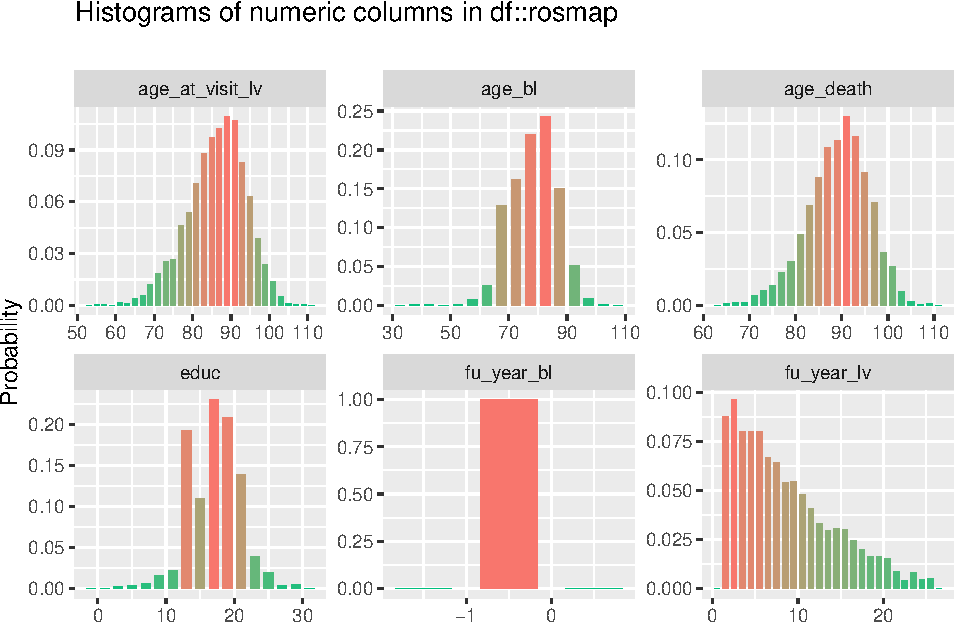
\includegraphics{notebook_files/figure-latex/unnamed-chunk-1-1.pdf}

\begin{Shaded}
\begin{Highlighting}[]
\NormalTok{demo_c }\OperatorTok\StringTok{ }\KeywordTok{show_plot}\NormalTok{(}\DataTypeTok{high_cardinality =} \DecValTok{5}\NormalTok{)}
\end{Highlighting}
\end{Shaded}

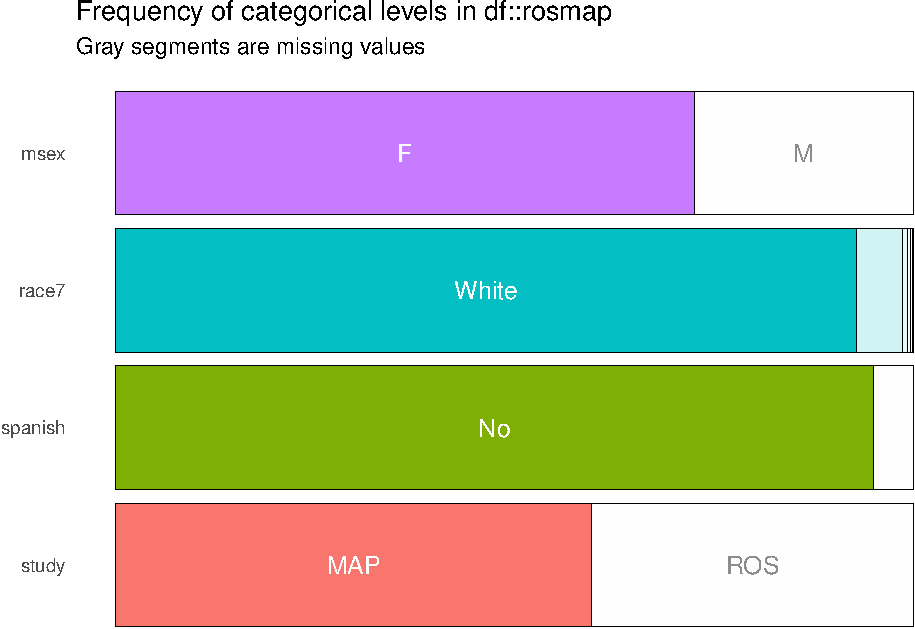
\includegraphics{notebook_files/figure-latex/unnamed-chunk-1-2.pdf}

\hypertarget{genetics}{%
\section{Genetics}\label{genetics}}

\label{tab:rosmap-genetic-global}Data Summary

variables

definitions

types

missing\_percent

unique\_count

Source.Tissue.Type

Source tissue for DNA

character

67.89

15

organ

collapsed source tissue into organ

factor

67.89

4

apoe\_genotype

APOE genotypes

factor

14.30

7

apoe4

APOE e4 carriers

factor

14.30

3

tomm40\_hap

TOMM40 genotype

factor

36.19

7

\label{tab:rosmap-genetic-factor}Variable type: Factor

col\_name

level

prop

cnt

apoe\_genotype

33

0.53

1947

apoe\_genotype

34

0.18

665

apoe\_genotype

NA

0.14

525

apoe\_genotype

23

0.11

390

apoe\_genotype

24

0.02

72

apoe\_genotype

44

0.02

56

apoe\_genotype

22

0.00

17

apoe4

e4-

0.64

2354

apoe4

e4+

0.22

793

apoe4

NA

0.14

525

organ

NA

0.68

2493

organ

brain

0.22

796

organ

blood

0.10

378

organ

lymphocytes

0.00

5

Source.Tissue.Type

NA

0.68

2493

Source.Tissue.Type

Brain-DLPFC

0.13

460

Source.Tissue.Type

Whole Blood

0.10

355

Source.Tissue.Type

Brain-Cerebellum

0.07

256

Source.Tissue.Type

Brain-Posterior Cingulate Cortex

0.02

67

Source.Tissue.Type

Other

0.01

41

tomm40\_hap

NA

0.36

1329

tomm40\_hap

S/VL

0.23

833

tomm40\_hap

S/S

0.13

485

tomm40\_hap

VL/VL

0.13

469

tomm40\_hap

S/L

0.07

269

tomm40\_hap

L/VL

0.07

250

tomm40\_hap

L/L

0.01

37

\hypertarget{plots-1}{%
\subsection{Plots}\label{plots-1}}

\begin{Shaded}
\begin{Highlighting}[]
\NormalTok{genetic_c }\OperatorTok\StringTok{ }\KeywordTok{show_plot}\NormalTok{(}\DataTypeTok{high_cardinality =} \DecValTok{5}\NormalTok{)}
\end{Highlighting}
\end{Shaded}

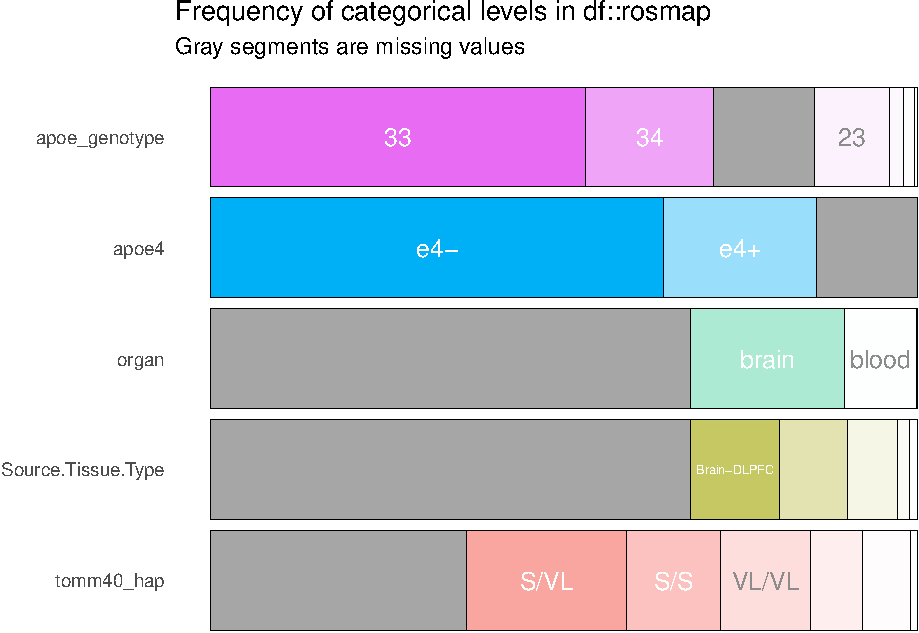
\includegraphics{notebook_files/figure-latex/unnamed-chunk-2-1.pdf}

\hypertarget{mitochondria}{%
\section{Mitochondria}\label{mitochondria}}

\label{tab:mt-numeric}Variable type: Numeric

col\_name

min

q1

median

mean

q3

max

sd

pcnt\_na

autosomal\_coverage

26.90

33.74

36.41

36.59

39.18

60.26

4.45

67.89

mt\_coverage

580.79

10127.78

25800.50

31538.67

53264.42

88911.89

23864.72

67.89

mtcn\_avg

41.37

564.44

1418.11

1735.36

2945.84

4988.99

1306.14

67.89

Quality

0.50

0.90

0.93

0.93

0.96

1.00

0.05

67.89

\label{tab:rosmap-mt-factor}Variable type: Factor

col\_name

level

prop

cnt

Haplogroup

NA

0.68

2493

Haplogroup

Other

0.27

987

Haplogroup

\href{mailto:V+@72}{\nolinkurl{V+@72}}

0.01

35

Haplogroup

H1

0.01

24

Haplogroup

H

0.01

22

Haplogroup

HV

0.01

19

Haplogroup

T2b

0.01

19

Haplogroup

T1a1

0.00

17

Haplogroup

H1a

0.00

16

Haplogroup

U5a1

0.00

16

Haplogroup

H1c

0.00

12

Haplogroup

J1c

0.00

12

macro

NA

0.68

2493

macro

H

0.14

507

macro

U

0.05

187

macro

T

0.03

111

macro

J

0.03

105

macro

K

0.02

78

macro

V

0.01

54

macro

I

0.01

37

macro

HV

0.01

35

macro

Other

0.01

26

macro

X

0.01

21

macro

W

0.00

18

\hypertarget{plots-2}{%
\subsection{Plots}\label{plots-2}}

\begin{Shaded}
\begin{Highlighting}[]
\NormalTok{mt_n }\OperatorTok\StringTok{ }\KeywordTok{show_plot}\NormalTok{()}
\end{Highlighting}
\end{Shaded}

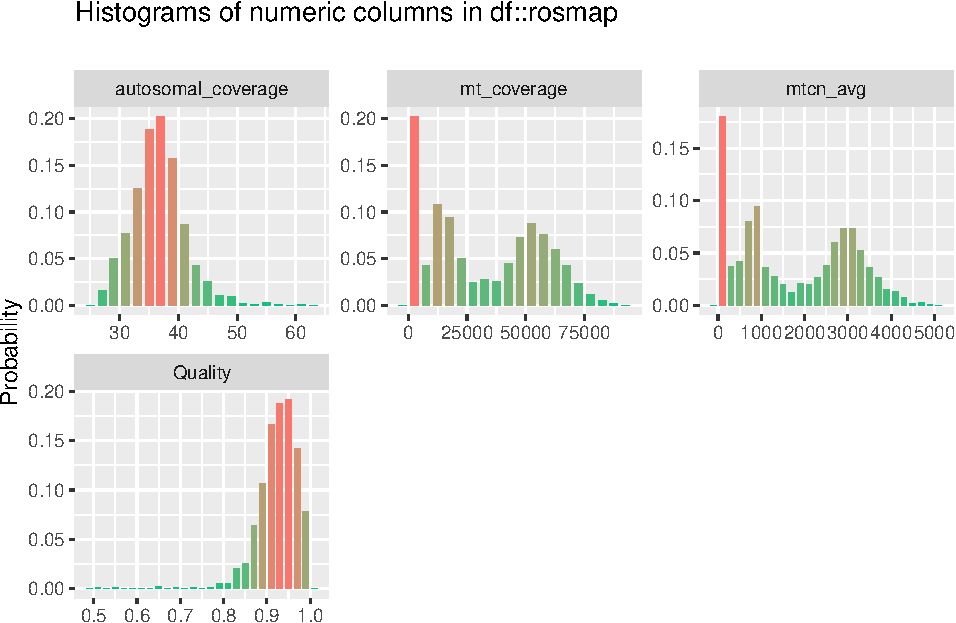
\includegraphics{notebook_files/figure-latex/mt-plots-1.pdf}

\begin{Shaded}
\begin{Highlighting}[]
\NormalTok{mt_c }\OperatorTok\StringTok{ }\KeywordTok{show_plot}\NormalTok{(}\DataTypeTok{high_cardinality =} \DecValTok{5}\NormalTok{)}
\end{Highlighting}
\end{Shaded}

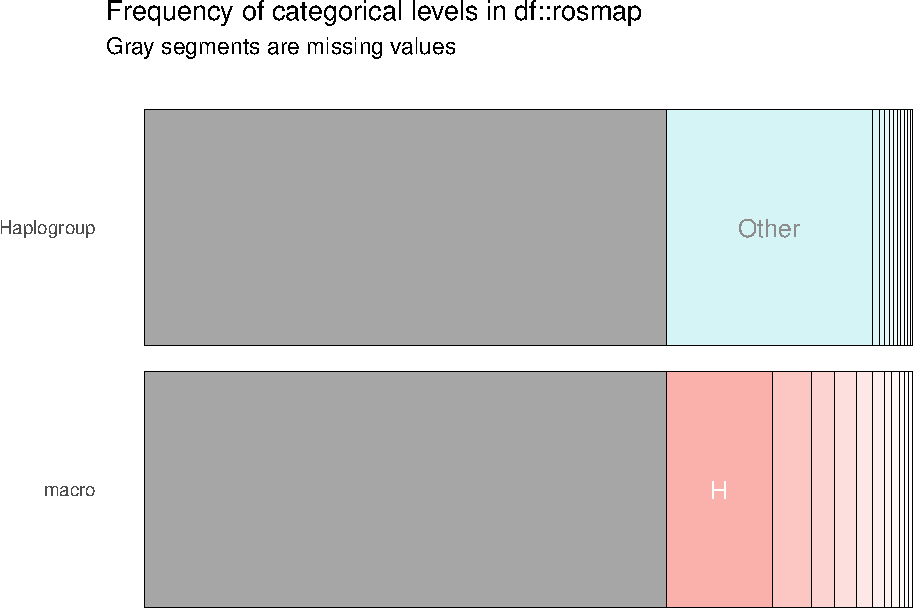
\includegraphics{notebook_files/figure-latex/mt-plots-2.pdf}

\hypertarget{diagnosis-and-mtdnacn}{%
\subsection{diagnosis and mtDNAcn}\label{diagnosis-and-mtdnacn}}

\begin{Shaded}
\begin{Highlighting}[]
\NormalTok{mtcn_dx <-}\StringTok{ }\NormalTok{rosmap }\OperatorTok
\StringTok{    }\KeywordTok{filter}\NormalTok{(}\OperatorTok{!}\KeywordTok{is.na}\NormalTok{(mtcn_avg)) }\OperatorTok
\StringTok{    }\KeywordTok{mutate}\NormalTok{(}\DataTypeTok{Source.Tissue.Type =} \KeywordTok{fct_lump_n}\NormalTok{(Source.Tissue.Type, }\DecValTok{5}\NormalTok{), }
      \DataTypeTok{dx_lv =} \KeywordTok{fct_recode}\NormalTok{(dcfdx_lv, }\StringTok{"CTRL"}\NormalTok{ =}\StringTok{ "1"}\NormalTok{, }
                            \StringTok{"MCI"}\NormalTok{ =}\StringTok{ "2"}\NormalTok{, }\StringTok{"MCI"}\NormalTok{ =}\StringTok{ "3"}\NormalTok{, }
                            \StringTok{"AD"}\NormalTok{ =}\StringTok{ "4"}\NormalTok{, }\StringTok{"AD"}\NormalTok{ =}\StringTok{ "5"}\NormalTok{, }\StringTok{"AD"}\NormalTok{ =}\StringTok{ "6"}\NormalTok{), }
         \DataTypeTok{dx_bl =} \KeywordTok{fct_recode}\NormalTok{(dcfdx_bl, }\StringTok{"CTRL"}\NormalTok{ =}\StringTok{ "1"}\NormalTok{, }
                            \StringTok{"MCI"}\NormalTok{ =}\StringTok{ "2"}\NormalTok{, }\StringTok{"MCI"}\NormalTok{ =}\StringTok{ "3"}\NormalTok{, }
                            \StringTok{"AD"}\NormalTok{ =}\StringTok{ "4"}\NormalTok{, }\StringTok{"AD"}\NormalTok{ =}\StringTok{ "5"}\NormalTok{, }\StringTok{"AD"}\NormalTok{ =}\StringTok{ "6"}\NormalTok{)) }

\NormalTok{mtcn_dx }\OperatorTok
\StringTok{  }\KeywordTok{ggplot}\NormalTok{(., }\KeywordTok{aes}\NormalTok{(}\DataTypeTok{x =}\NormalTok{ Source.Tissue.Type, }\DataTypeTok{y =}\NormalTok{ mtcn_avg, }\DataTypeTok{colour =}\NormalTok{ dx_bl)) }\OperatorTok{+}\StringTok{ }
\StringTok{    }\NormalTok{ggbeeswarm}\OperatorTok{::}\KeywordTok{geom_quasirandom}\NormalTok{(}\DataTypeTok{dodge.width=}\DecValTok{1}\NormalTok{) }\OperatorTok{+}\StringTok{ }
\StringTok{    }\KeywordTok{facet_grid}\NormalTok{(organ }\OperatorTok{~}\StringTok{ }\NormalTok{., }\DataTypeTok{scales =} \StringTok{"free"}\NormalTok{) }\OperatorTok{+}\StringTok{ }
\StringTok{  }\KeywordTok{theme_bw}\NormalTok{()}
\end{Highlighting}
\end{Shaded}

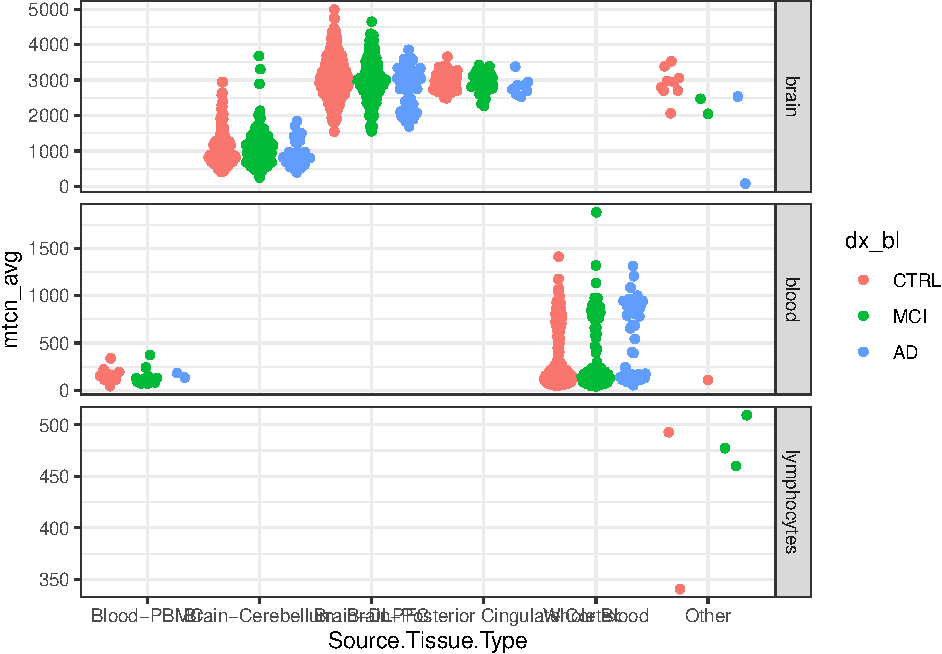
\includegraphics{notebook_files/figure-latex/dx-mtdnacn-1.pdf}

\begin{Shaded}
\begin{Highlighting}[]
\NormalTok{mtcn_dx }\OperatorTok
\StringTok{  }\KeywordTok{ggplot}\NormalTok{(., }\KeywordTok{aes}\NormalTok{(}\DataTypeTok{x =}\NormalTok{ Source.Tissue.Type, }\DataTypeTok{y =}\NormalTok{ mtcn_avg, }\DataTypeTok{colour =}\NormalTok{ r_pd_lv)) }\OperatorTok{+}\StringTok{ }
\StringTok{    }\NormalTok{ggbeeswarm}\OperatorTok{::}\KeywordTok{geom_quasirandom}\NormalTok{(}\DataTypeTok{dodge.width=}\DecValTok{1}\NormalTok{) }\OperatorTok{+}\StringTok{ }
\StringTok{    }\KeywordTok{facet_grid}\NormalTok{(organ }\OperatorTok{~}\StringTok{ }\NormalTok{., }\DataTypeTok{scales =} \StringTok{"free"}\NormalTok{) }\OperatorTok{+}\StringTok{ }
\StringTok{  }\KeywordTok{theme_bw}\NormalTok{()}
\end{Highlighting}
\end{Shaded}

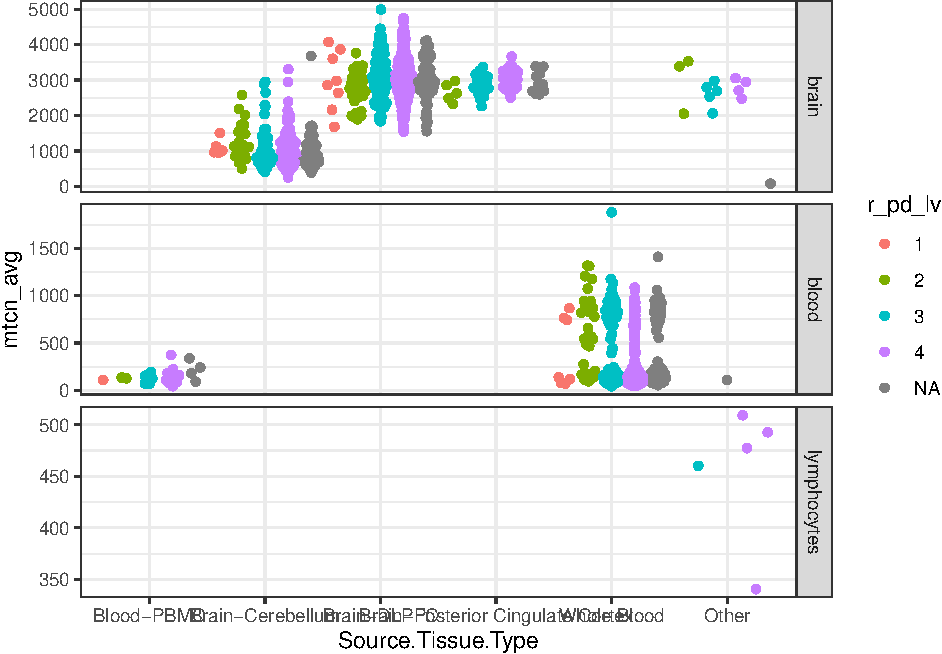
\includegraphics{notebook_files/figure-latex/dx-mtdnacn-2.pdf}

\hypertarget{blood-cell-counts-and-mtdnacn}{%
\subsection{Blood cell counts and mtDNAcn}\label{blood-cell-counts-and-mtdnacn}}

\begin{itemize}
\tightlist
\item
  mtDNAcn estimates from whole blood DNA can be confounded by cell type heterogeneity, and by the presence of platelets, as platelets do not have nDNA, but have mtDNA, which artificially inflates mtDNAcn. \href{https://dx.doi.org/10.1016/j.psyneuen.2019.04.004}{Han, L. et al 2019}
\item
  A subset of patients in ROSMAP have longitudinal measures of blood cell counts - can test if bimodal distribution of mtDNAcn in whole blood is due to cell type heterogeneity
\end{itemize}

\begin{Shaded}
\begin{Highlighting}[]
\NormalTok{blood_mt <-}\StringTok{ }\NormalTok{rosmap }\OperatorTok
\StringTok{  }\KeywordTok{mutate}\NormalTok{(}\DataTypeTok{dx_lv =} \KeywordTok{fct_recode}\NormalTok{(dcfdx_lv, }\StringTok{"CTRL"}\NormalTok{ =}\StringTok{ "1"}\NormalTok{, }
                            \StringTok{"MCI"}\NormalTok{ =}\StringTok{ "2"}\NormalTok{, }\StringTok{"MCI"}\NormalTok{ =}\StringTok{ "3"}\NormalTok{, }
                            \StringTok{"AD"}\NormalTok{ =}\StringTok{ "4"}\NormalTok{, }\StringTok{"AD"}\NormalTok{ =}\StringTok{ "5"}\NormalTok{, }\StringTok{"AD"}\NormalTok{ =}\StringTok{ "6"}\NormalTok{), }
         \DataTypeTok{dx_bl =} \KeywordTok{fct_recode}\NormalTok{(dcfdx_bl, }\StringTok{"CTRL"}\NormalTok{ =}\StringTok{ "1"}\NormalTok{, }
                            \StringTok{"MCI"}\NormalTok{ =}\StringTok{ "2"}\NormalTok{, }\StringTok{"MCI"}\NormalTok{ =}\StringTok{ "3"}\NormalTok{, }
                            \StringTok{"AD"}\NormalTok{ =}\StringTok{ "4"}\NormalTok{, }\StringTok{"AD"}\NormalTok{ =}\StringTok{ "5"}\NormalTok{, }\StringTok{"AD"}\NormalTok{ =}\StringTok{ "6"}\NormalTok{)) }\OperatorTok\StringTok{ }
\StringTok{  }\KeywordTok{select}\NormalTok{(projid, study, Source.Tissue.Type,}
\NormalTok{         age_at_visit_bl, age_at_visit_lv,}
\NormalTok{         platelet_bl, rbc_bl, rdw_bl, wbc_bl,}
\NormalTok{         platelet_lv, rbc_lv, rdw_lv, wbc_lv,}
\NormalTok{         dx_bl, dx_lv,}
\NormalTok{         mtcn_avg) }\OperatorTok\StringTok{ }
\StringTok{  }\KeywordTok{pivot_longer}\NormalTok{(}\KeywordTok{c}\NormalTok{(}\OperatorTok{-}\NormalTok{study, }\OperatorTok{-}\NormalTok{Source.Tissue.Type, }\OperatorTok{-}\NormalTok{projid, }\OperatorTok{-}\NormalTok{mtcn_avg, }\OperatorTok{-}\NormalTok{dx_lv, }\OperatorTok{-}\NormalTok{dx_bl, }\OperatorTok{-}\NormalTok{age_at_visit_bl, }\OperatorTok{-}\NormalTok{age_at_visit_lv), }
               \DataTypeTok{names_to =} \StringTok{"cells"}\NormalTok{, }\DataTypeTok{values_to =} \StringTok{"value"}\NormalTok{)}
  
\NormalTok{blood_mt }\OperatorTok\StringTok{ }
\StringTok{  }\KeywordTok{filter}\NormalTok{(Source.Tissue.Type }\OperatorTok{==}\StringTok{ "Whole Blood"}\NormalTok{) }\OperatorTok
\StringTok{  }\KeywordTok{filter}\NormalTok{(}\KeywordTok{str_detect}\NormalTok{(cells, }\StringTok{"platelet_lv|rbc_lv|rdw_lv|wbc_lv"}\NormalTok{)) }\OperatorTok
\StringTok{  }\KeywordTok{ggplot}\NormalTok{(., }\KeywordTok{aes}\NormalTok{(}\DataTypeTok{x =}\NormalTok{ value, }\DataTypeTok{y =}\NormalTok{ mtcn_avg, }\DataTypeTok{colour =}\NormalTok{ dx_lv)) }\OperatorTok{+}\StringTok{ }
\StringTok{    }\KeywordTok{facet_grid}\NormalTok{(. }\OperatorTok{~}\StringTok{ }\NormalTok{cells, }\DataTypeTok{scales =} \StringTok{"free"}\NormalTok{) }\OperatorTok{+}\StringTok{ }
\StringTok{    }\KeywordTok{geom_point}\NormalTok{() }\OperatorTok{+}\StringTok{ }
\StringTok{    }\KeywordTok{theme_bw}\NormalTok{() }\OperatorTok{+}\StringTok{ }
\StringTok{    }\KeywordTok{theme}\NormalTok{(}\DataTypeTok{legend.position =} \StringTok{"bottom"}\NormalTok{)}
\end{Highlighting}
\end{Shaded}

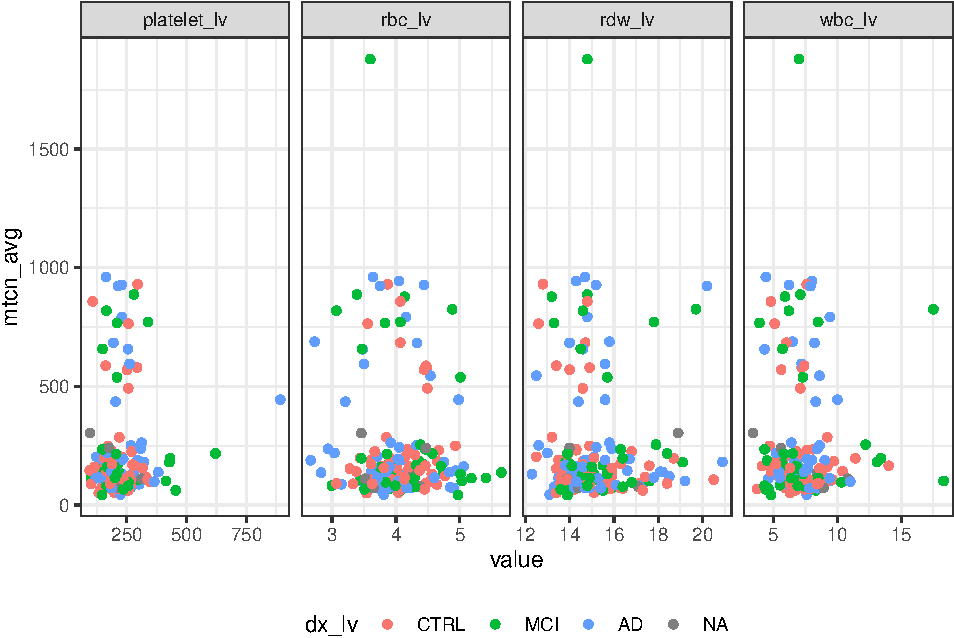
\includegraphics{notebook_files/figure-latex/blood-mt-1.pdf}

\begin{Shaded}
\begin{Highlighting}[]
\NormalTok{blood_mt }\OperatorTok\StringTok{ }
\StringTok{  }\KeywordTok{filter}\NormalTok{(Source.Tissue.Type }\OperatorTok{==}\StringTok{ "Whole Blood"}\NormalTok{) }\OperatorTok
\StringTok{  }\KeywordTok{filter}\NormalTok{(}\KeywordTok{str_detect}\NormalTok{(cells, }\StringTok{"platelet_bl|rbc_bl|rdw_bl|wbc_bl"}\NormalTok{)) }\OperatorTok
\StringTok{  }\KeywordTok{ggplot}\NormalTok{(., }\KeywordTok{aes}\NormalTok{(}\DataTypeTok{x =}\NormalTok{ value, }\DataTypeTok{y =}\NormalTok{ mtcn_avg, }\DataTypeTok{colour =}\NormalTok{ dx_lv)) }\OperatorTok{+}\StringTok{ }
\StringTok{    }\KeywordTok{facet_grid}\NormalTok{(. }\OperatorTok{~}\StringTok{ }\NormalTok{cells, }\DataTypeTok{scales =} \StringTok{"free"}\NormalTok{) }\OperatorTok{+}\StringTok{ }
\StringTok{    }\KeywordTok{geom_point}\NormalTok{() }\OperatorTok{+}
\StringTok{    }\KeywordTok{theme_bw}\NormalTok{() }\OperatorTok{+}\StringTok{ }
\StringTok{    }\KeywordTok{theme}\NormalTok{(}\DataTypeTok{legend.position =} \StringTok{"bottom"}\NormalTok{)}
\end{Highlighting}
\end{Shaded}

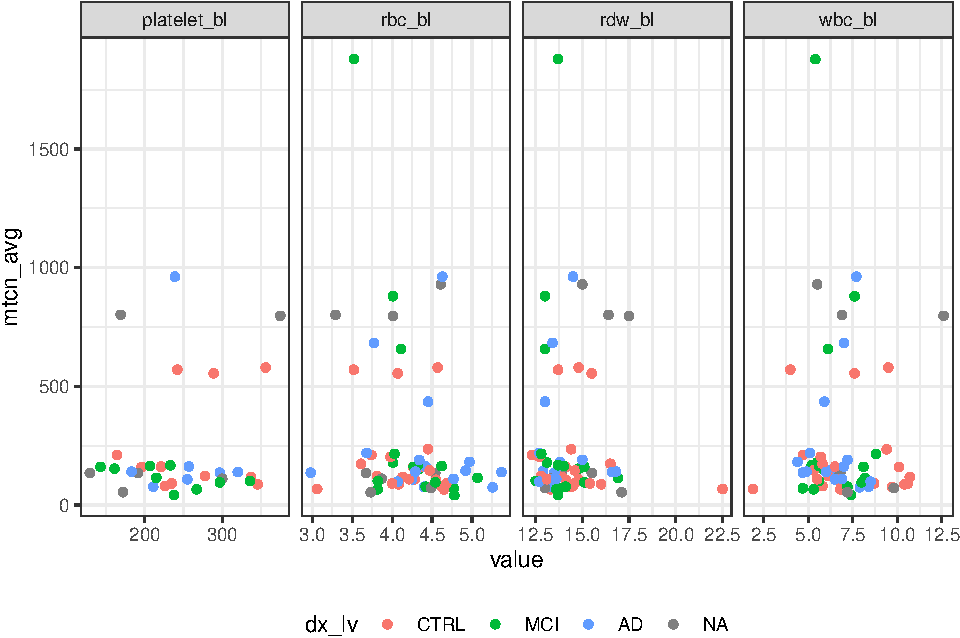
\includegraphics{notebook_files/figure-latex/blood-mt-2.pdf}

\hypertarget{rna-seq}{%
\section{RNA-seq}\label{rna-seq}}

\begin{itemize}
\tightlist
\item
  Neuronal and astrocyte cell type enrichment are estimated using xCell to adjust
  for potential neuronal cell loss in dementia
\item
  Only avaliable in a subset of participants
\end{itemize}

\label{tab:rosmap-rna-numeric}Variable type: Numeric

col\_name

min

q1

median

mean

q3

max

sd

pcnt\_na

Neurons

0.00

0.05

0.06

0.06

0.07

0.09

0.02

82.41

Astrocytes

0.01

0.02

0.03

0.03

0.04

0.09

0.01

82.41

RIN

5.00

6.30

7.20

7.06

7.90

9.90

1.00

82.43

\textbf{Characteristic}

DLPFC

Unknown

\textbf{Total}

\textbf{Source.Tissue.Type}

Blood

0 (0\%)

1 (\textless{}0.1\%)

1 (\textless{}0.1\%)

Blood-Cerebellum

0 (0\%)

1 (\textless{}0.1\%)

1 (\textless{}0.1\%)

Blood-PBMC

0 (0\%)

22 (0.6\%)

22 (0.6\%)

Brain-Anterior Caudate

2 (\textless{}0.1\%)

2 (\textless{}0.1\%)

4 (0.1\%)

Brain-Cerebellum

111 (3.0\%)

145 (3.9\%)

256 (7.0\%)

Brain-DLPFC

217 (5.9\%)

243 (6.6\%)

460 (13\%)

Brain-Frontal Cortex (BA unknown)

0 (0\%)

1 (\textless{}0.1\%)

1 (\textless{}0.1\%)

Brain-Frontal Pole (BA10-12,32)

0 (0\%)

1 (\textless{}0.1\%)

1 (\textless{}0.1\%)

Brain-Occipital Association Cortex (BA18,19)

2 (\textless{}0.1\%)

2 (\textless{}0.1\%)

4 (0.1\%)

Brain-PCC

0 (0\%)

1 (\textless{}0.1\%)

1 (\textless{}0.1\%)

Brain-Posterior Cingulate Cortex

62 (1.7\%)

5 (0.1\%)

67 (1.8\%)

Brain-region unknown

0 (0\%)

1 (\textless{}0.1\%)

1 (\textless{}0.1\%)

lymphocytes \_transformed \_with EBV virus

2 (\textless{}0.1\%)

3 (\textless{}0.1\%)

5 (0.1\%)

Whole Blood

188 (5.1\%)

167 (4.5\%)

355 (9.7\%)

Unknown

62 (1.7\%)

2,431 (66\%)

2,493 (68\%)

\textbf{Total}

646 (18\%)

3,026 (82\%)

3,672 (100\%)

\hypertarget{plots-3}{%
\subsection{Plots}\label{plots-3}}

\begin{Shaded}
\begin{Highlighting}[]
\NormalTok{rna_n }\OperatorTok\StringTok{ }\KeywordTok{show_plot}\NormalTok{()}
\end{Highlighting}
\end{Shaded}

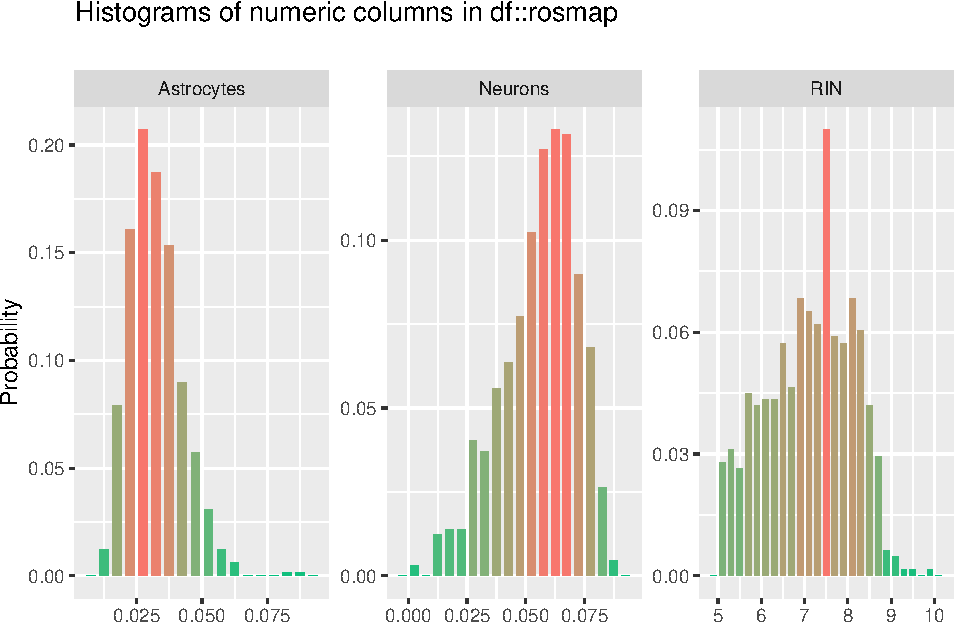
\includegraphics{notebook_files/figure-latex/rosmap-rna-plots-1.pdf}

\begin{Shaded}
\begin{Highlighting}[]
\NormalTok{rosmap_xcell <-}\StringTok{ }\KeywordTok{select}\NormalTok{(rosmap, Neurons, Astrocytes, rna_seq_tissue, Source.Tissue.Type, }
\NormalTok{                       age_death, cogdx, ad_reagan, mtcn_avg, msex}
\NormalTok{                       ) }\OperatorTok\StringTok{ }
\StringTok{  }\KeywordTok{mutate}\NormalTok{(}\DataTypeTok{ad_reagan =} \KeywordTok{as_factor}\NormalTok{(ad_reagan)) }\OperatorTok
\StringTok{  }\KeywordTok{filter}\NormalTok{(}\OperatorTok{!}\KeywordTok{is.na}\NormalTok{(Neurons)) }\OperatorTok\StringTok{ }
\StringTok{  }\KeywordTok{pivot_longer}\NormalTok{(}\KeywordTok{c}\NormalTok{(Neurons, Astrocytes), }\DataTypeTok{names_to =} \StringTok{"cells"}\NormalTok{, }\DataTypeTok{values_to =} \StringTok{"xcell"}\NormalTok{)}

\KeywordTok{ggplot}\NormalTok{(rosmap_xcell, }\KeywordTok{aes}\NormalTok{(}\DataTypeTok{x =}\NormalTok{ cogdx, }\DataTypeTok{y =}\NormalTok{ xcell, }\DataTypeTok{colour =}\NormalTok{ cells)) }\OperatorTok{+}\StringTok{ }
\StringTok{  }\NormalTok{ggbeeswarm}\OperatorTok{::}\KeywordTok{geom_quasirandom}\NormalTok{(}\DataTypeTok{dodge.width=}\DecValTok{1}\NormalTok{) }\OperatorTok{+}\StringTok{ }
\StringTok{  }\KeywordTok{theme_bw}\NormalTok{()}
\end{Highlighting}
\end{Shaded}

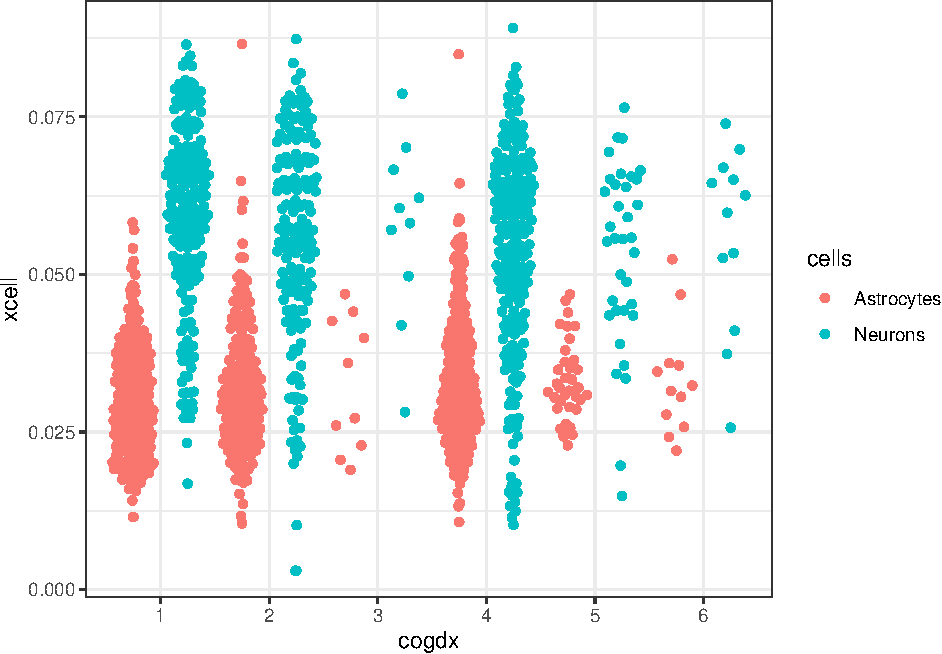
\includegraphics{notebook_files/figure-latex/rosmap-rna-dx-plots-1.pdf}

\begin{Shaded}
\begin{Highlighting}[]
\KeywordTok{ggplot}\NormalTok{(rosmap_xcell, }\KeywordTok{aes}\NormalTok{(}\DataTypeTok{x =}\NormalTok{ ad_reagan, }\DataTypeTok{y =}\NormalTok{ xcell, }\DataTypeTok{colour =}\NormalTok{ cells)) }\OperatorTok{+}\StringTok{ }
\StringTok{  }\CommentTok{# facet_grid(. ~ cells) + }
\StringTok{  }\NormalTok{ggbeeswarm}\OperatorTok{::}\KeywordTok{geom_quasirandom}\NormalTok{(}\DataTypeTok{dodge.width=}\DecValTok{1}\NormalTok{) }\OperatorTok{+}\StringTok{ }
\StringTok{  }\KeywordTok{theme_bw}\NormalTok{()}
\end{Highlighting}
\end{Shaded}

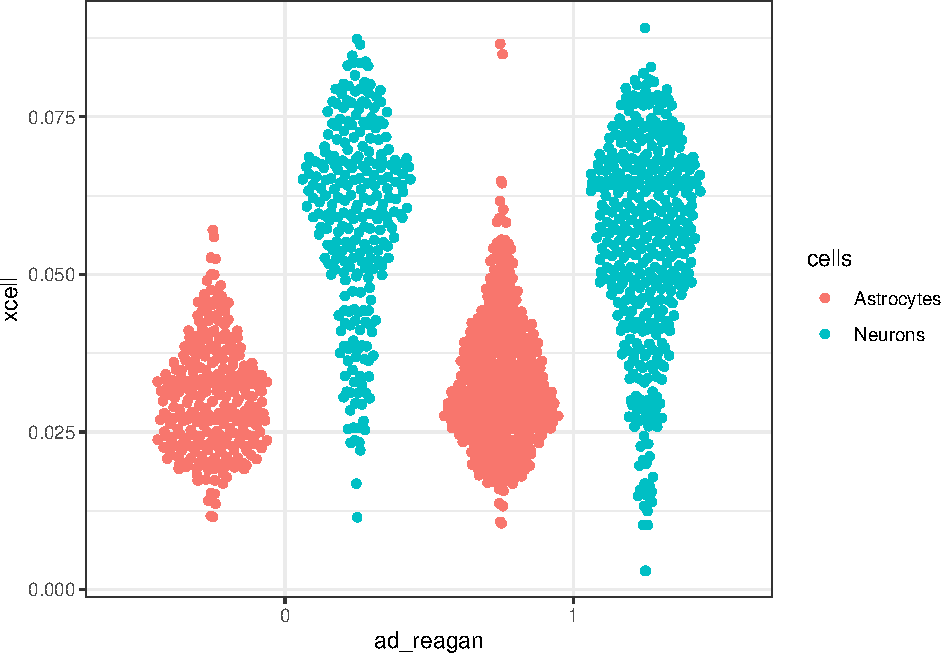
\includegraphics{notebook_files/figure-latex/rosmap-rna-dx-plots-2.pdf}

\begin{Shaded}
\begin{Highlighting}[]
\KeywordTok{ggplot}\NormalTok{(rosmap_xcell, }\KeywordTok{aes}\NormalTok{(}\DataTypeTok{x =}\NormalTok{ msex, }\DataTypeTok{y =}\NormalTok{ xcell, }\DataTypeTok{colour =}\NormalTok{ cells)) }\OperatorTok{+}\StringTok{ }
\StringTok{  }\CommentTok{# facet_grid(. ~ cells) + }
\StringTok{  }\NormalTok{ggbeeswarm}\OperatorTok{::}\KeywordTok{geom_quasirandom}\NormalTok{(}\DataTypeTok{dodge.width=}\DecValTok{1}\NormalTok{) }\OperatorTok{+}\StringTok{ }
\StringTok{  }\KeywordTok{theme_bw}\NormalTok{()}
\end{Highlighting}
\end{Shaded}

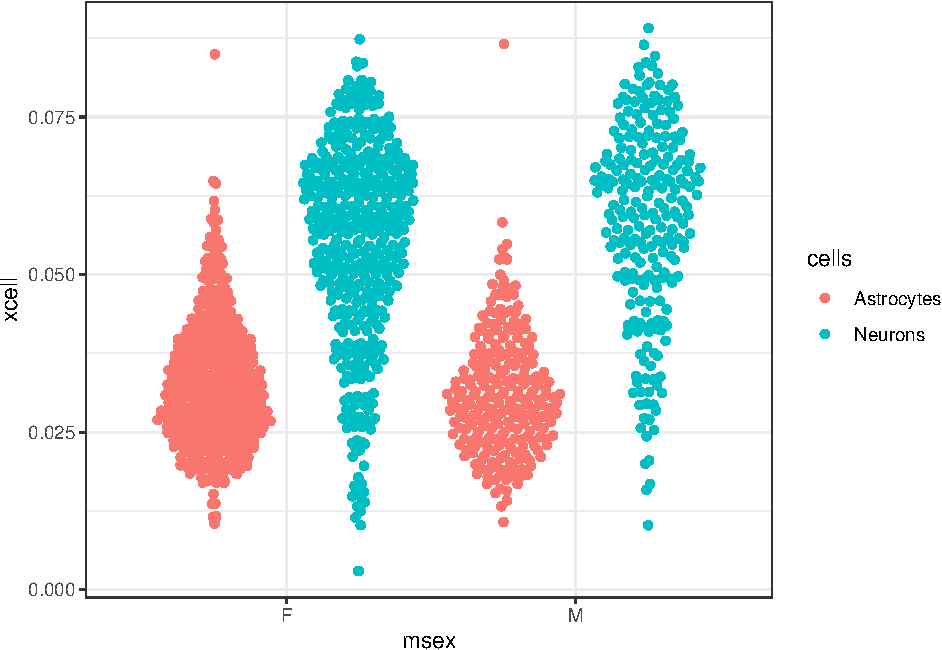
\includegraphics{notebook_files/figure-latex/rosmap-rna-dx-plots-3.pdf}

\begin{Shaded}
\begin{Highlighting}[]
\KeywordTok{ggplot}\NormalTok{(rosmap_xcell, }\KeywordTok{aes}\NormalTok{(}\DataTypeTok{x =}\NormalTok{ age_death, }\DataTypeTok{y =}\NormalTok{ xcell, }\DataTypeTok{colour =}\NormalTok{ ad_reagan)) }\OperatorTok{+}\StringTok{ }
\StringTok{  }\KeywordTok{facet_grid}\NormalTok{(. }\OperatorTok{~}\StringTok{ }\NormalTok{cells) }\OperatorTok{+}
\StringTok{  }\KeywordTok{geom_point}\NormalTok{() }\OperatorTok{+}\StringTok{ }
\StringTok{  }\KeywordTok{geom_smooth}\NormalTok{(}\DataTypeTok{method =}\NormalTok{ lm) }\OperatorTok{+}\StringTok{ }
\StringTok{  }\KeywordTok{theme_bw}\NormalTok{()}
\end{Highlighting}
\end{Shaded}

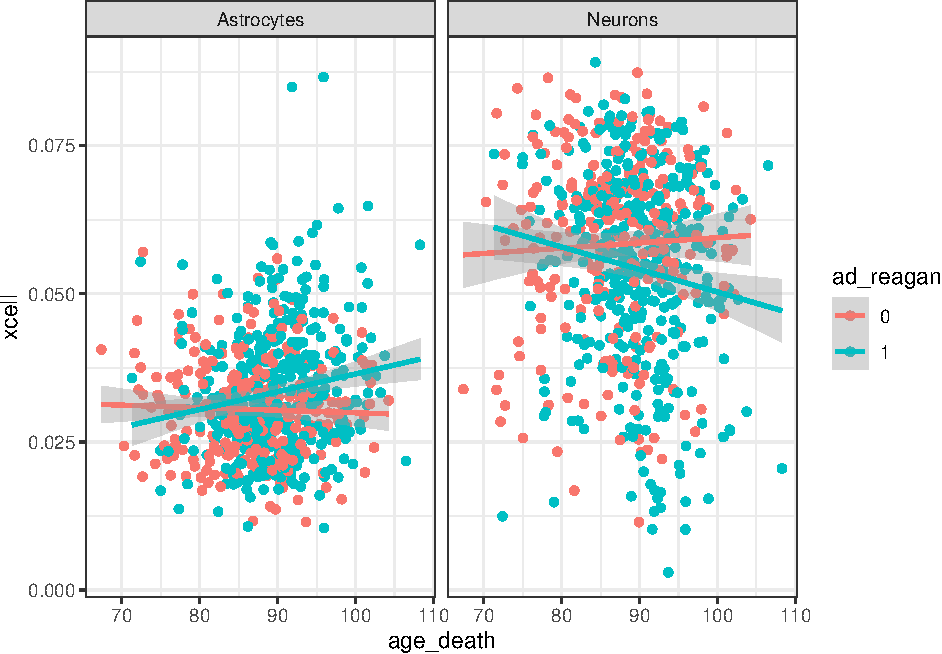
\includegraphics{notebook_files/figure-latex/rosmap-rna-dx-plots-4.pdf}

\begin{Shaded}
\begin{Highlighting}[]
\NormalTok{rosmap_xcell }\OperatorTok\StringTok{ }
\StringTok{  }\KeywordTok{filter}\NormalTok{(Source.Tissue.Type }\OperatorTok{==}\StringTok{ "Brain-DLPFC"}\NormalTok{) }\OperatorTok
\KeywordTok{ggplot}\NormalTok{(., }\KeywordTok{aes}\NormalTok{(}\DataTypeTok{x =}\NormalTok{ mtcn_avg, }\DataTypeTok{y =}\NormalTok{ xcell, }\DataTypeTok{colour =}\NormalTok{ cogdx)) }\OperatorTok{+}\StringTok{ }
\StringTok{  }\KeywordTok{facet_grid}\NormalTok{(. }\OperatorTok{~}\StringTok{ }\NormalTok{cells) }\OperatorTok{+}
\StringTok{  }\KeywordTok{geom_point}\NormalTok{() }\OperatorTok{+}\StringTok{ }
\StringTok{  }\KeywordTok{geom_smooth}\NormalTok{(}\DataTypeTok{method =}\NormalTok{ lm) }\OperatorTok{+}\StringTok{ }
\StringTok{  }\KeywordTok{theme_bw}\NormalTok{()}
\end{Highlighting}
\end{Shaded}

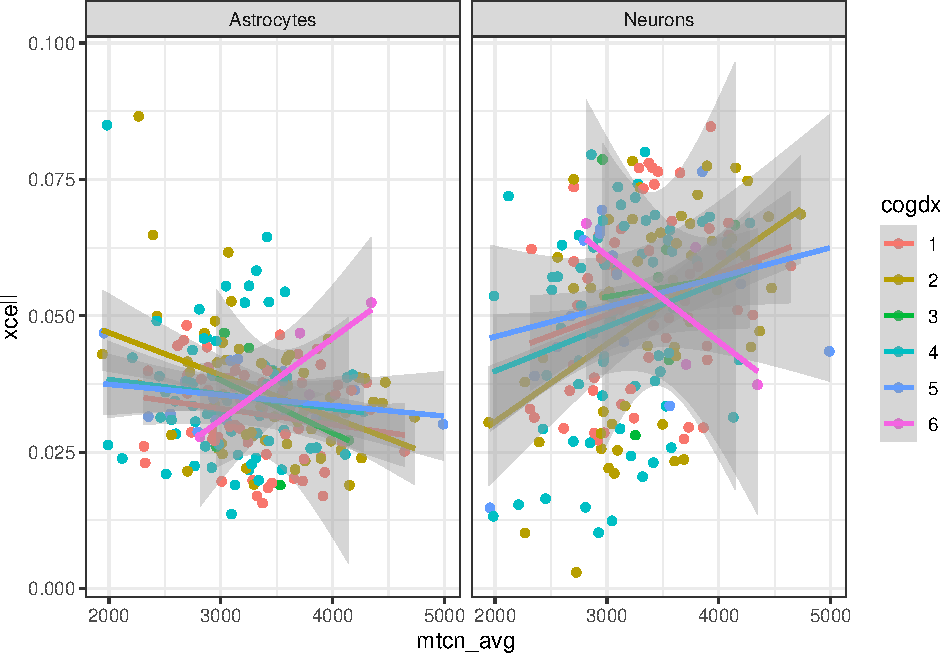
\includegraphics{notebook_files/figure-latex/rosmap-rna-dx-plots-5.pdf}

\hypertarget{clinical-diagnosis}{%
\section{Clinical Diagnosis}\label{clinical-diagnosis}}

\begin{itemize}
\tightlist
\item
  \href{https://www.radc.rush.edu/docs/var/detail.htm?category=Clinical+Diagnosis\&subcategory=Final+consensus+diagnosis\&variable=cogdx}{Clinical cognitive diagnosis summary}: \texttt{dcfdx} Physician's overall cognitive diagnostic category

  \begin{itemize}
  \tightlist
  \item
    1 = NCI: No cognitive impairment (No impaired domains)
  \item
    2 = MCI: Mild cognitive impairment (One impaired domain) and NO other cause of CI
  \item
    3 = MCI: Mild cognitive impairment (One impaired domain) AND another cause of CI
  \item
    4 = AD: Alzheimer's dementia and NO other cause of CI (NINCDS PROB AD)
  \item
    5 = AD: Alzheimer's dementia AND another cause of CI (NINCDS POSS AD)
  \item
    6 = Other dementia: Other primary cause of dementia
  \end{itemize}
\item
  \href{https://www.radc.rush.edu/docs/var/detail.htm?category=Clinical+Diagnosis\&subcategory=Dementia\&variable=age_first_ad_dx}{Age at first Alzheimer's dementia dx}: \texttt{age\_first\_ad\_dx} Age at cycle where first Alzheimer's dementia diagnosis was given
\item
  \href{https://www.radc.rush.edu/docs/var/detail.htm?category=Clinical+Diagnosis\&subcategory=Final+consensus+diagnosis\&variable=cogdx}{Final consensus cognitive diagnosis}: \texttt{cogdx} Clinical consensus diagnosis of cognitive status at time of death - same coding as \texttt{dcfdx}
\item
  \href{https://www.radc.rush.edu/docs/var/detail.htm?category=Clinical+Diagnosis\&subcategory=Parkinson\%27s+disease\&variable=r_pd}{Clinical Parkinson's disease}: \texttt{r\_pd} is made by a clinician through review of self report questions, neurological exam (when available), cognitive testing, and interview of participant.

  \begin{itemize}
  \tightlist
  \item
    1 = Highly Probable
  \item
    2 = Probable
  \item
    3 = Possible
  \item
    4 = Not Present
  \end{itemize}
\item
  \href{https://www.radc.rush.edu/docs/var/detail.htm?category=Clinical+Diagnosis\&subcategory=Stroke\&variable=r_stroke}{Stroke diagnosis}: \texttt{r\_stroke} s made by a clinician through review of self report questions, neurological exam (when available), cognitive testing, and interview of participant.

  \begin{itemize}
  \tightlist
  \item
    1 = Highly Probable
  \item
    2 = Probable
  \item
    3 = Possible
  \item
    4 = Not Present
  \end{itemize}
\end{itemize}

\label{tab:rosmap-dx}Data Summary

variables

definitions

types

missing\_percent

unique\_count

cogdx

Clinical consensus diagnosis of cognitive status at time of death

factor

46.00

7

age\_first\_ad\_dx

Age at cycle where first Alzheimer's dementia diagnosis was given

numeric

75.95

838

dcfdx\_bl

Physician's overall cognitive diagnostic category - baseline

factor

0.03

7

dcfdx\_lv

Physician's overall cognitive diagnostic category - last visit

factor

17.10

7

r\_pd\_bl

Diagnosis of Parkinson's disease - baseline

factor

1.39

6

r\_pd\_lv

Diagnosis of Parkinson's disease - last visit

factor

38.26

6

r\_stroke\_bl

Diagnosis of stroke made by clinician - baseline

factor

6.92

5

r\_stroke\_lv

Diagnosis of stroke made by clinician - last visit

factor

28.70

5

\label{tab:rosmap-dx-numeric}Variable type: Numeric

col\_name

min

q1

median

mean

q3

max

sd

pcnt\_na

age\_first\_ad\_dx

64.06

83.4

87.93

87.56

92.16

107.23

6.58

75.95

\label{tab:rosmap-dx-factor}Variable type: Factor

col\_name

level

prop

cnt

cogdx

NA

0.46

1689

4

0.20

732

1

0.17

641

2

0.12

440

5

0.03

103

3

0.01

36

6

0.01

31

dcfdx\_bl

1

0.69

2545

2

0.24

896

4

0.05

196

6

0.00

12

3

0.00

11

5

0.00

11

NA

0.00

1

dcfdx\_lv

1

0.39

1433

4

0.21

787

2

0.18

654

NA

0.17

628

5

0.03

105

6

0.01

44

3

0.01

21

r\_pd\_bl

4

0.83

3056

3

0.13

463

2

0.02

80

NA

0.01

51

1

0.01

21

9

0.00

1

r\_pd\_lv

4

0.44

1633

NA

0.38

1405

3

0.12

436

2

0.04

165

1

0.01

31

8

0.00

2

r\_stroke\_bl

4

0.80

2949

NA

0.07

254

2

0.06

221

3

0.05

184

1

0.02

64

r\_stroke\_lv

4

0.67

2443

NA

0.29

1054

3

0.02

73

2

0.02

72

1

0.01

30

\hypertarget{plots-4}{%
\subsection{Plots}\label{plots-4}}

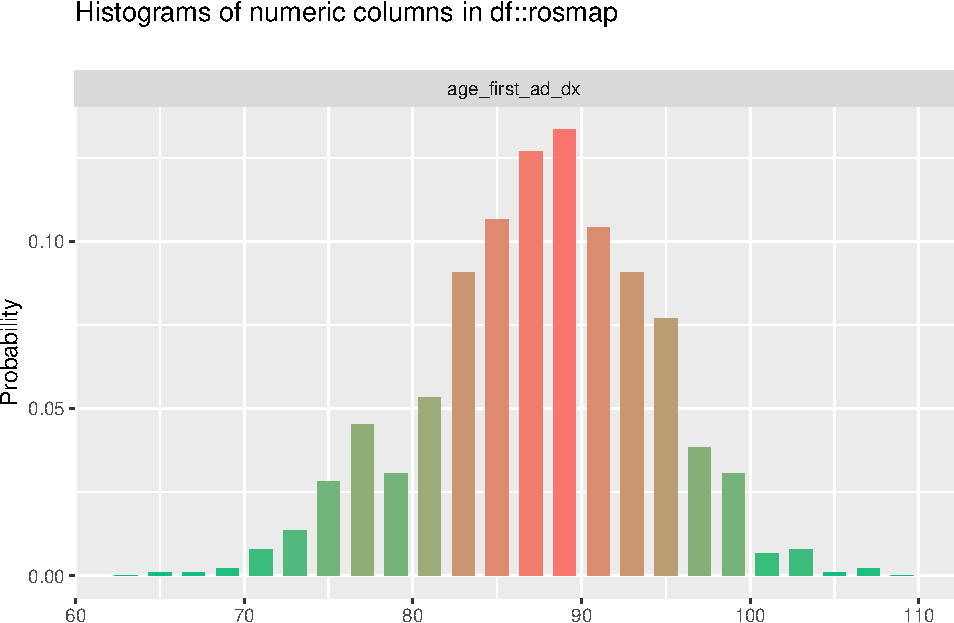
\includegraphics{notebook_files/figure-latex/unnamed-chunk-4-1.pdf} 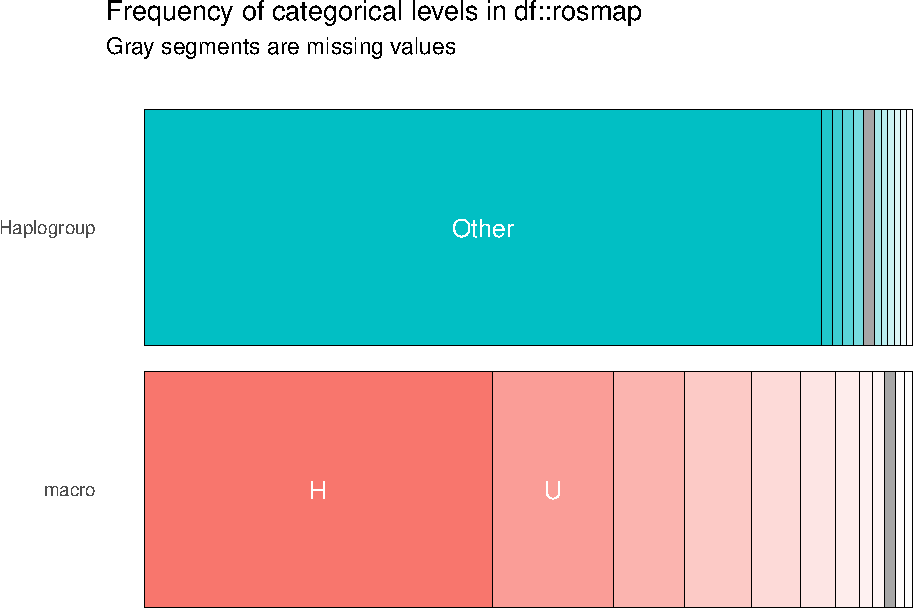
\includegraphics{notebook_files/figure-latex/unnamed-chunk-4-2.pdf}

\hypertarget{cross-tabs}{%
\subsection{Cross-tabs}\label{cross-tabs}}

\textbf{Characteristic}

1

2

3

4

5

6

Unknown

\textbf{Total}

\textbf{cogdx}

1

535 (15\%)

22 (0.6\%)

0 (0\%)

1 (\textless{}0.1\%)

0 (0\%)

2 (\textless{}0.1\%)

81 (2.2\%)

641 (17\%)

2

19 (0.5\%)

362 (9.9\%)

5 (0.1\%)

1 (\textless{}0.1\%)

0 (0\%)

0 (0\%)

53 (1.4\%)

440 (12\%)

3

6 (0.2\%)

18 (0.5\%)

8 (0.2\%)

1 (\textless{}0.1\%)

0 (0\%)

0 (0\%)

3 (\textless{}0.1\%)

36 (1.0\%)

4

1 (\textless{}0.1\%)

20 (0.5\%)

0 (0\%)

593 (16\%)

29 (0.8\%)

9 (0.2\%)

80 (2.2\%)

732 (20\%)

5

0 (0\%)

0 (0\%)

0 (0\%)

31 (0.8\%)

51 (1.4\%)

14 (0.4\%)

7 (0.2\%)

103 (2.8\%)

6

1 (\textless{}0.1\%)

0 (0\%)

1 (\textless{}0.1\%)

9 (0.2\%)

6 (0.2\%)

12 (0.3\%)

2 (\textless{}0.1\%)

31 (0.8\%)

Unknown

871 (24\%)

232 (6.3\%)

7 (0.2\%)

151 (4.1\%)

19 (0.5\%)

7 (0.2\%)

402 (11\%)

1,689 (46\%)

\textbf{Total}

1,433 (39\%)

654 (18\%)

21 (0.6\%)

787 (21\%)

105 (2.9\%)

44 (1.2\%)

628 (17\%)

3,672 (100\%)

\hypertarget{pathology}{%
\section{Pathology}\label{pathology}}

\href{https://www.radc.rush.edu/docs/var/overview.htm?category=Pathology}{Pathology}: post-mortem neuropathologic evaluation

\begin{itemize}
\tightlist
\item
  Alzheimer's disease

  \begin{itemize}
  \tightlist
  \item
    \href{https://www.radc.rush.edu/docs/var/detail.htm?category=Pathology\&subcategory=Alzheimer\%27s+disease\&variable=niareagansc}{NIA-Reagan diagnosis of AD}: \texttt{niareagansc} modified NIA-Reagan diagnosis of Alzheimer's disease is based on consensus recommendations for postmortem diagnosis of Alzheimer's disease. The criteria rely on both neurofibrillary tangles (Braak) and neuritic plaques (CERAD).

    \begin{itemize}
    \tightlist
    \item
      1 = High; 2 = Intermediate; 3 = Low; 4 = No AD
    \end{itemize}
  \item
    Dichomtomized NIA-Reagan: \texttt{ad\_reagan}
  \item
    \href{https://www.radc.rush.edu/docs/var/detail.htm?category=Pathology\&subcategory=Alzheimer\%27s+disease\&variable=ceradsc}{CERAD score}: \texttt{ceradsc} CERAD score is a semiquantitative measure of neuritic plaques. A CERAD neuropathologic diagnosis of AD required moderate (probable AD) or frequent neuritic plaques (definite AD) in one or more neocortical regions.

    \begin{itemize}
    \tightlist
    \item
      1 = Definite -\textgreater{} frequent (C3); 2 = Probable -\textgreater{} moderate (C2); 3 = Possible -\textgreater{} Sparse (C1); 4 = No AD -\textgreater{} None (C0)
    \end{itemize}
  \item
    \href{https://www.radc.rush.edu/docs/var/detail.htm?category=Pathology\&subcategory=Alzheimer\%27s+disease\&variable=braaksc}{Braak stage}: \texttt{braaksc} Braak Stage is a semiquantitative measure of severity of neurofibrillary tangle (NFT) pathology.

    \begin{itemize}
    \tightlist
    \item
      0 = 0; 1 = I (entorhinal); 2 = II (entorhinal); 3 = III (limbic); 4 = IV (limbic); 5 = V (neocortical); 6 = VI (neocortical)
    \end{itemize}
  \item
    \href{https://www.radc.rush.edu/docs/var/detail.htm?category=Pathology\&subcategory=Alzheimer\%27s+disease\&variable=gpath}{Global AD pathology burden}: \texttt{gpath} Global AD pathology burden is a quantitative summary of AD pathology derived from counts of three AD pathologies: neuritic plaques (n), diffuse plaques (d), and neurofibrillary tangles (nft)
  \end{itemize}
\item
  Beta-Amyloid

  \begin{itemize}
  \tightlist
  \item
    \href{https://www.radc.rush.edu/docs/var/detail.htm?category=Pathology\&subcategory=Beta-Amyloid\&variable=amyloid}{amyloid}: \texttt{amyloid} Overall amyloid level - Mean of 8 brain regions
  \item
    \href{https://www.radc.rush.edu/docs/var/detail.htm?category=Pathology\&subcategory=Beta-Amyloid\&variable=plaq_d}{plaq\_d}: \texttt{plaq\_d} Diffuse plaque summary based on 5 regions
  \item
    \href{https://www.radc.rush.edu/docs/var/detail.htm?category=Pathology\&subcategory=Beta-Amyloid\&variable=plaq_n}{plaq\_n}: \texttt{plaq\_n} Neuritic plaque summary based on 5 regions
  \end{itemize}
\item
  PHF tau Tangles

  \begin{itemize}
  \tightlist
  \item
    \href{https://www.radc.rush.edu/docs/var/detail.htm?category=Pathology\&subcategory=PHF+tau+tangles\&variable=tangles}{Tangle}: \texttt{tangles} Tangle density - Mean of 8 brain regions
  \item
    \href{https://www.radc.rush.edu/docs/var/detail.htm?category=Pathology\&subcategory=PHF+tau+tangles\&variable=nft}{NFT burden}: \texttt{nft} Neurofibrillary tangle summary based on 5 regions
  \end{itemize}
\item
  \href{https://www.radc.rush.edu/docs/var/detail.htm?category=Pathology\&subcategory=Lewy+body\%2fPD\&variable=dlbdx}{Lewy Body disease}: \texttt{dlbdx} Pathologic diagnosis of Lewy body diseases - 4 stages

  \begin{itemize}
  \tightlist
  \item
    0 = Not present; 1 = nigral-predominant; 2 = limbic-type; 3 = neocortical-type
  \end{itemize}
\item
  Vascular

  \begin{itemize}
  \tightlist
  \item
    \href{https://www.radc.rush.edu/docs/var/detail.htm?category=Pathology\&subcategory=Vascular+-+Infarcts+(Presence+of)\&variable=ci_num2_gct}{gross infarcts}: \texttt{ci\_num\_gct} Cerebral Infarctions - Binary - Gross-Chronic-Any Location
  \item
    \href{https://www.radc.rush.edu/docs/var/detail.htm?category=Pathology\&subcategory=Vascular+-+Infarcts+(Presence+of)\&variable=ci_num2_mct}{micro infarcts}: \texttt{ci\_num2\_mct} Cerebral Infarctions - Binary - Micro-Chronic-Any Location
  \item
    \href{https://www.radc.rush.edu/docs/var/detail.htm?category=Pathology\&subcategory=Vascular+-+General+measures\&variable=cvda_4gp2}{Cerebral atherosclerosis}: \texttt{cvda\_4gp2} Cerebral Atherosclerosis Rating

    \begin{itemize}
    \tightlist
    \item
      0 = None; 1 = Mild; 2 = Moderate; 3 = Severe
    \end{itemize}
  \item
    \href{https://www.radc.rush.edu/docs/var/detail.htm?category=Pathology\&subcategory=Vascular+-+General+measures\&variable=caa_4gp}{Cerebral amyloid angiopathy}: \texttt{caa\_4gp} Cerebral amyloid angiopathy

    \begin{itemize}
    \tightlist
    \item
      0 = None; 1 = Mild; 2 = Moderate; 3 = Severe
    \end{itemize}
  \item
    \href{https://www.radc.rush.edu/docs/var/detail.htm?category=Pathology\&subcategory=Vascular+-+General+measures\&variable=arteriol_scler}{Arteriolosclerosis}: \texttt{arteriol\_scler} Arteriolosclerosis

    \begin{itemize}
    \tightlist
    \item
      0 = None; 1 = Mild; 2 = Moderate; 3 = Severe
    \end{itemize}
  \end{itemize}
\item
  \href{https://www.radc.rush.edu/docs/var/detail.htm?category=Pathology\&subcategory=Hippocampal+sclerosis\&variable=hspath_typ}{Hippocampal sclerosis (Typical)}: \texttt{hspath\_typ} Definite presence of typical hippocampal sclerosis
\item
  \href{https://www.radc.rush.edu/docs/var/detail.htm?category=Pathology\&subcategory=TDP-43\&variable=tdp_st4}{TDP-43 stage}: \texttt{tdp\_st4} TDP-43 pathology from 8 regions

  \begin{itemize}
  \tightlist
  \item
    0 = None; 1 = Amygdala; 2 = Amygdala + Limbic; 3 = Amygdala + Limbic + Neocortical
  \item
    dichotomized version: 0 = No TDP-43 pathology or TDP-43 pathology in amygdala only (Stages 0 and 1); 1 = TDP-43 pathology extending beyond amygdala (Stages 2 and 3)
  \end{itemize}
\item
  \href{https://www.radc.rush.edu/docs/var/overview.htm?category=Pathology\&subcategory=Microglia}{Microglia}: Immunohistochemistry for microglia

  \begin{itemize}
  \tightlist
  \item
    mglia123\_caud\_vm
  \item
    mglia123\_it
  \item
    mglia123\_mf
  \item
    mglia123\_put\_p
  \item
    mglia23\_caud\_vm
  \item
    mglia23\_it
  \item
    mglia23\_mf
  \item
    mglia23\_put\_p
  \item
    mglia3\_caud\_vm
  \item
    mglia3\_it
  \item
    mglia3\_mf
  \item
    mglia3\_put\_p
  \end{itemize}
\end{itemize}

\label{tab:rosmap-path}Data Summary

variables

definitions

types

missing\_percent

unique\_count

niareagansc

NA

ordered

53.76

5

ceradsc

NA

ordered

53.76

5

braaksc

NA

ordered

53.76

8

gpath

NA

numeric

53.95

1605

amyloid

NA

numeric

55.47

1374

plaq\_d

NA

numeric

53.95

1308

plaq\_n

NA

numeric

53.95

1264

tangles

NA

numeric

55.28

1622

nft

NA

numeric

53.95

1368

dlbdx

NA

factor

55.23

5

ci\_num2\_gct

NA

factor

53.79

3

ci\_num2\_mct

NA

factor

53.79

3

cvda\_4gp2

NA

factor

53.40

5

caa\_4gp

NA

factor

54.90

5

arteriol\_scler

NA

factor

54.08

5

hspath\_typ

NA

factor

56.05

3

tdp\_st4

NA

factor

56.86

5

\label{tab:rosmap-path-numeric}Variable type: Numeric

col\_name

min

q1

median

mean

q3

max

sd

pcnt\_na

gpath

0

0.19

0.64

0.75

1.14

3.20

0.63

53.95

amyloid

0

0.53

2.83

3.93

6.24

22.94

3.95

55.47

plaq\_d

0

0.09

0.53

0.73

1.10

4.93

0.77

53.95

plaq\_n

0

0.06

0.71

0.86

1.34

5.36

0.84

53.95

tangles

0

1.59

4.23

7.28

9.46

78.52

8.83

55.28

nft

0

0.14

0.37

0.65

0.85

6.10

0.78

53.95

\hypertarget{htmlwidget-4b6080d63955848b42f4}{}
\begin{datatables}

\end{datatables}

\hypertarget{plots-5}{%
\subsection{Plots}\label{plots-5}}

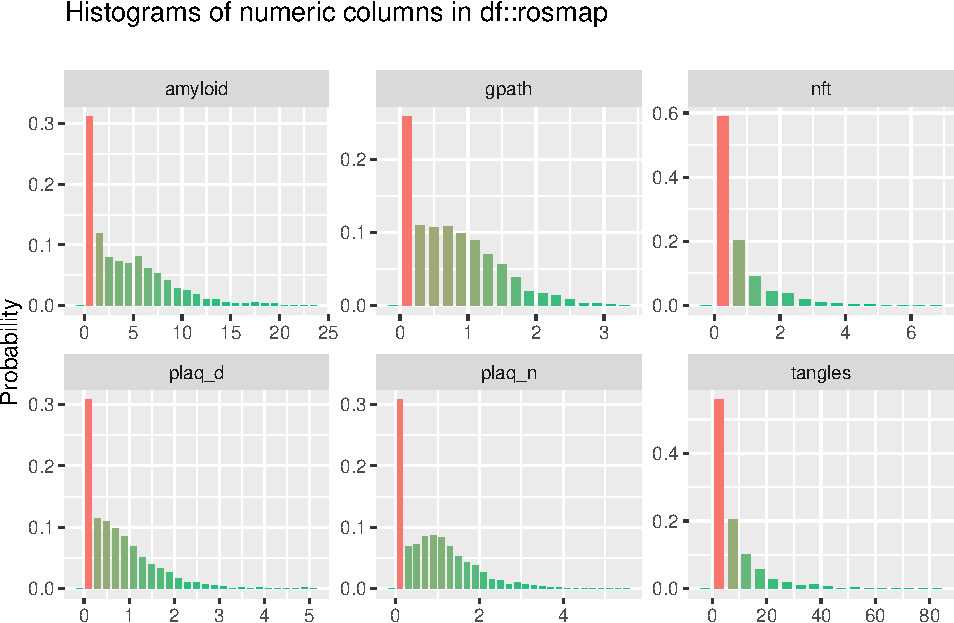
\includegraphics{notebook_files/figure-latex/rosmap-inspect-plot-1.pdf} 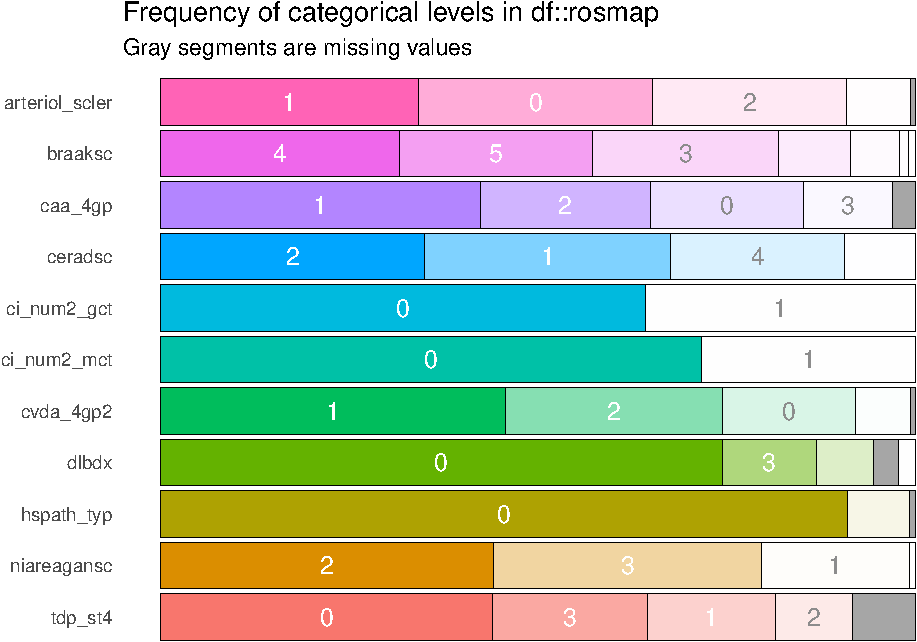
\includegraphics{notebook_files/figure-latex/rosmap-inspect-plot-2.pdf}

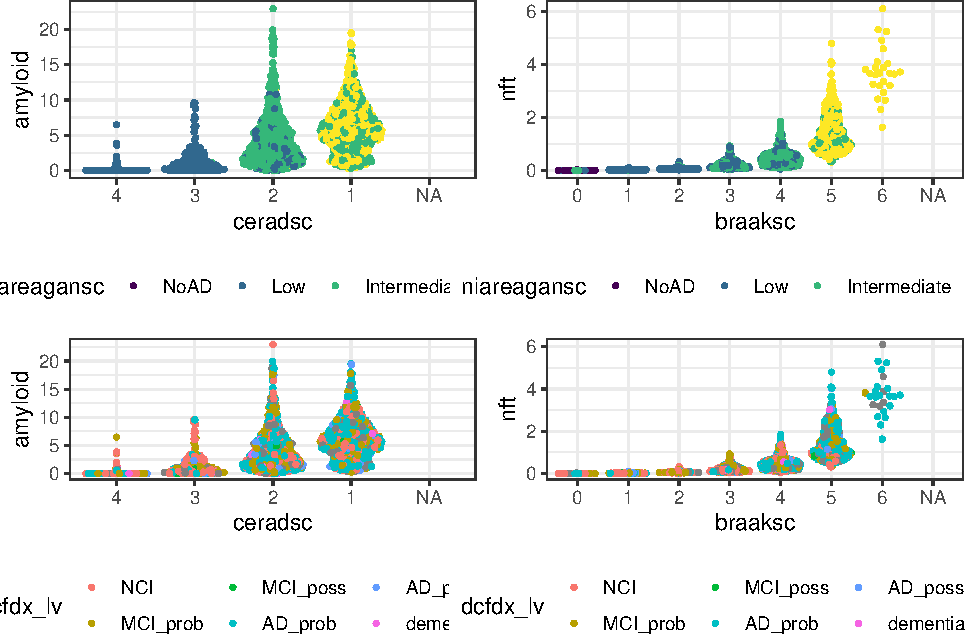
\includegraphics{notebook_files/figure-latex/rosmap-path-dx-plot-1.pdf}

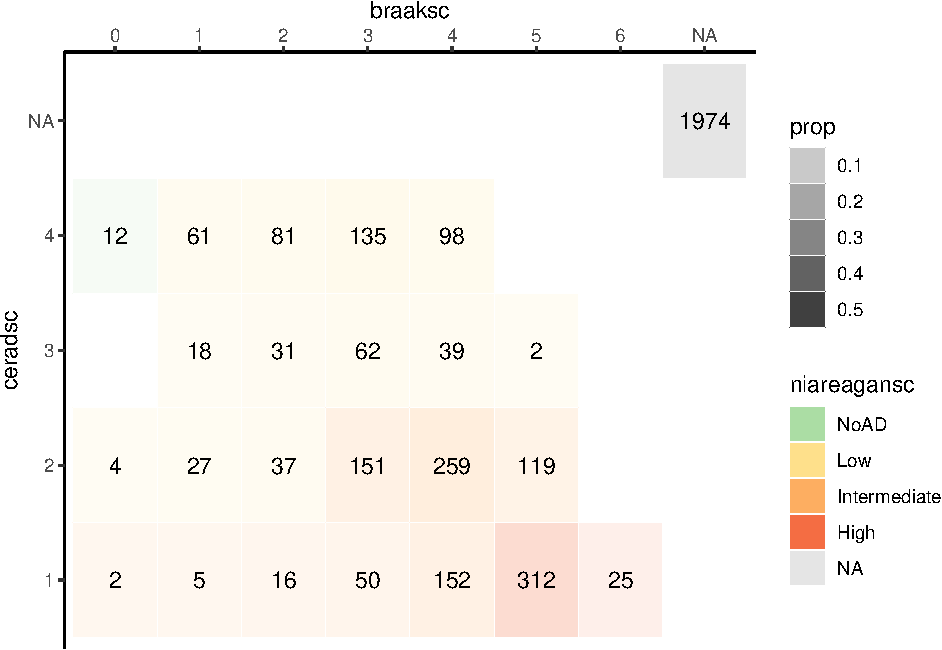
\includegraphics{notebook_files/figure-latex/rosmap-path-crosstab-plot-1.pdf}

\hypertarget{cross-tabs-1}{%
\subsection{Cross-Tabs}\label{cross-tabs-1}}

\textbf{Characteristic}

0

1

2

3

4

5

6

Unknown

\textbf{Total}

\textbf{ceradsc}

1

2 (\textless{}0.1\%)

5 (0.1\%)

16 (0.4\%)

50 (1.4\%)

152 (4.1\%)

312 (8.5\%)

25 (0.7\%)

0 (0\%)

562 (15\%)

2

4 (0.1\%)

27 (0.7\%)

37 (1.0\%)

151 (4.1\%)

259 (7.1\%)

119 (3.2\%)

0 (0\%)

0 (0\%)

597 (16\%)

3

0 (0\%)

18 (0.5\%)

31 (0.8\%)

62 (1.7\%)

39 (1.1\%)

2 (\textless{}0.1\%)

0 (0\%)

0 (0\%)

152 (4.1\%)

4

12 (0.3\%)

61 (1.7\%)

81 (2.2\%)

135 (3.7\%)

98 (2.7\%)

0 (0\%)

0 (0\%)

0 (0\%)

387 (11\%)

Unknown

0 (0\%)

0 (0\%)

0 (0\%)

0 (0\%)

0 (0\%)

0 (0\%)

0 (0\%)

1,974 (54\%)

1,974 (54\%)

\textbf{Total}

18 (0.5\%)

111 (3.0\%)

165 (4.5\%)

398 (11\%)

548 (15\%)

433 (12\%)

25 (0.7\%)

1,974 (54\%)

3,672 (100\%)

\textbf{Characteristic}

4

3

2

1

Unknown

\textbf{Total}

\textbf{cogdx}

1

8 (1.2\%)

301 (47\%)

207 (32\%)

24 (3.7\%)

101 (16\%)

641 (100\%)

2

4 (0.9\%)

133 (30\%)

181 (41\%)

45 (10\%)

77 (18\%)

440 (100\%)

3

0 (0\%)

19 (53\%)

10 (28\%)

2 (5.6\%)

5 (14\%)

36 (100\%)

4

0 (0\%)

92 (13\%)

302 (41\%)

247 (34\%)

91 (12\%)

732 (100\%)

5

0 (0\%)

35 (34\%)

37 (36\%)

21 (20\%)

10 (9.7\%)

103 (100\%)

6

0 (0\%)

14 (45\%)

12 (39\%)

3 (9.7\%)

2 (6.5\%)

31 (100\%)

Unknown

0 (0\%)

0 (0\%)

1 (\textless{}0.1\%)

0 (0\%)

1,688 (100\%)

1,689 (100\%)

\textbf{Total}

12 (0.3\%)

594 (16\%)

750 (20\%)

342 (9.3\%)

1,974 (54\%)

3,672 (100\%)

ceradsc

braaksc

NoAD

Low

Intermediate

High

NA

C0

B0

12

NA

NA

NA

NA

B1

NA

142

NA

NA

NA

B2

NA

233

NA

NA

NA

C1

B1

NA

49

NA

NA

NA

B2

NA

100

1

NA

NA

B3

NA

2

NA

NA

NA

C2

B0

NA

4

NA

NA

NA

B1

NA

63

1

NA

NA

B2

NA

1

409

NA

NA

B3

NA

NA

115

4

NA

C3

B0

NA

NA

2

NA

NA

B1

NA

NA

21

NA

NA

B2

NA

NA

201

1

NA

B3

NA

NA

NA

337

NA

\hypertarget{cognition}{%
\section{Cognition}\label{cognition}}

\begin{itemize}
\tightlist
\item
  \href{https://www.radc.rush.edu/docs/var/detail.htm?category=Cognition\&subcategory=Test+scores\&variable=cts_mmse30}{mmse}: Mini Mental State Examination is a widely used, 30 item, standardized screening measure of dementia severity. The MMSE can be used as a surrogate measure for the CDR for the staging of dementia in AD \href{https://doi.org/10.1097/01.JGP.0000192478.82189.a8}{Perneczky et al 2006}.
\end{itemize}

\begin{longtable}[]{@{}ll@{}}
\toprule
MMSE & CDR\tabularnewline
\midrule
\endhead
30 & 0 (No)\tabularnewline
26-29 & 0.5 (Questionable)\tabularnewline
21-25 & 1 (Mild)\tabularnewline
11-20 & 2 (Moderate)\tabularnewline
0-10 & 3 (Severe)\tabularnewline
\bottomrule
\end{longtable}

\begin{itemize}
\tightlist
\item
  Domains

  \begin{itemize}
  \tightlist
  \item
    \href{https://www.radc.rush.edu/docs/var/detail.htm?category=Cognition\&subcategory=Global+cognition\&variable=cogn_global}{Global cognitive function}: \texttt{cogn\_global}
  \item
    \href{https://www.radc.rush.edu/docs/var/detail.htm?category=Cognition\&subcategory=Domains\&variable=cogn_ep}{Episodic memory}: \texttt{cogn\_ep}
  \item
    \href{https://www.radc.rush.edu/docs/var/detail.htm?category=Cognition\&subcategory=Domains\&variable=cogn_wo}{Working memory}: \texttt{cogn\_wo}
  \item
    \href{https://www.radc.rush.edu/docs/var/detail.htm?category=Cognition\&subcategory=Domains\&variable=cogn_se}{Semantic memory}: \texttt{cogn\_se}
  \item
    \href{https://www.radc.rush.edu/docs/var/detail.htm?category=Cognition\&subcategory=Domains\&variable=cogn_po}{Perceptual orientation}: \texttt{cogn\_po}
  \item
    \href{https://www.radc.rush.edu/docs/var/detail.htm?category=Cognition\&subcategory=Domains\&variable=cogn_ps}{Perceptual speed}: \texttt{cogn\_ps}
  \end{itemize}
\item
  Estimated Slopes

  \begin{itemize}
  \tightlist
  \item
    \href{https://www.radc.rush.edu/docs/var/detail.htm?category=Cognition\&subcategory=Estimated+slopes\&variable=cogng_random_slope}{Global cognitive function}: \texttt{cogng\_random\_slope}
  \item
    \href{https://www.radc.rush.edu/docs/var/detail.htm?category=Cognition\&subcategory=Estimated+slopes\&variable=cognep_random_slope}{Episodic memory}: \texttt{cognep\_random\_slope}
  \item
    \href{https://www.radc.rush.edu/docs/var/detail.htm?category=Cognition\&subcategory=Estimated+slopes\&variable=cognwo_random_slope}{Working memory}: \texttt{cognwo\_random\_slope}
  \item
    \href{https://www.radc.rush.edu/docs/var/detail.htm?category=Cognition\&subcategory=Estimated+slopes\&variable=cognse_random_slope}{Semantic memory}: \texttt{cognse\_random\_slope}
  \item
    \href{https://www.radc.rush.edu/docs/var/detail.htm?category=Cognition\&subcategory=Estimated+slopes\&variable=cognpo_random_slope}{Perceptual orientation}: \texttt{cognpo\_random\_slope}
  \item
    \href{https://www.radc.rush.edu/docs/var/detail.htm?category=Cognition\&subcategory=Estimated+slopes\&variable=cognps_random_slope}{Perceptual speed}: \texttt{cognps\_random\_slope}
  \end{itemize}
\end{itemize}

\begin{verbatim}
# A tibble: 20 x 6
   variables       types  missing_count missing_percent unique_count unique_rate
   <chr>           <chr>          <int>           <dbl>        <int>       <dbl>
 1 cts_mmse30_bl   numer~             9           0.245           52      0.0142
 2 cogn_ep_bl      numer~            15           0.408         3606      0.982 
 3 cogn_po_bl      numer~            56           1.53           242      0.0659
 4 cogn_ps_bl      numer~            45           1.23          1093      0.298 
 5 cogn_se_bl      numer~            35           0.953         1197      0.326 
 6 cogn_wo_bl      numer~            11           0.300          645      0.176 
 7 cogn_global_bl  numer~             9           0.245         3648      0.993 
 8 cts_mmse30_lv   numer~           878          23.9            100      0.0272
 9 cogn_ep_lv      numer~          1210          33.0           2397      0.653 
10 cogn_po_lv      numer~          1390          37.9            243      0.0662
11 cogn_ps_lv      numer~          1298          35.3            982      0.267 
12 cogn_se_lv      numer~          1271          34.6           1216      0.331 
13 cogn_wo_lv      numer~           592          16.1            671      0.183 
14 cogn_global_lv  numer~           615          16.7           3034      0.826 
15 cognep_random_~ numer~           344           9.37          3315      0.903 
16 cogng_random_s~ numer~           300           8.17          3359      0.915 
17 cognpo_random_~ numer~           383          10.4           3276      0.892 
18 cognps_random_~ numer~           375          10.2           3284      0.894 
19 cognse_random_~ numer~           364           9.91          3295      0.897 
20 cognwo_random_~ numer~           299           8.14          3360      0.915 
\end{verbatim}

\label{tab:rosmap-cog-numeric}Variable type: Numeric

col\_name

min

q1

median

mean

q3

max

sd

pcnt\_na

cts\_mmse30\_bl

0.00

27.00

29.00

27.75

30.00

30.00

3.00

0.25

cogn\_ep\_bl

-4.06

-0.39

0.14

0.00

0.54

1.71

0.79

0.41

cogn\_po\_bl

-3.54

-0.61

0.05

0.00

0.63

1.59

0.85

1.53

cogn\_ps\_bl

-3.23

-0.55

0.07

-0.01

0.65

2.60

0.93

1.23

cogn\_se\_bl

-5.89

-0.37

0.13

0.00

0.51

2.32

0.76

0.95

cogn\_wo\_bl

-3.44

-0.54

-0.06

0.00

0.43

2.34

0.78

0.30

cogn\_global\_bl

-4.26

-0.35

0.09

-0.01

0.44

1.46

0.65

0.25

cts\_mmse30\_lv

0.00

20.00

26.79

22.66

29.00

30.00

8.53

23.91

cogn\_ep\_lv

-4.13

-1.22

-0.15

-0.42

0.52

1.92

1.26

32.95

cogn\_po\_lv

-3.54

-0.93

-0.16

-0.27

0.47

1.59

1.02

37.85

cogn\_ps\_lv

-3.23

-1.51

-0.54

-0.69

0.25

2.47

1.24

35.35

cogn\_se\_lv

-5.89

-0.86

-0.21

-0.46

0.30

3.23

1.15

34.61

cogn\_wo\_lv

-3.44

-0.86

-0.23

-0.36

0.26

2.67

1.01

16.12

cogn\_global\_lv

-4.24

-0.99

-0.21

-0.42

0.34

1.92

1.06

16.75

cognep\_random\_slope

-0.40

-0.04

0.02

0.00

0.06

0.23

0.09

9.37

cogng\_random\_slope

-0.48

-0.03

0.02

0.00

0.05

0.18

0.08

8.17

cognpo\_random\_slope

-0.20

-0.01

0.00

0.00

0.02

0.11

0.04

10.43

cognps\_random\_slope

-0.42

-0.03

0.01

0.00

0.04

0.21

0.07

10.21

cognse\_random\_slope

-0.74

-0.02

0.02

0.00

0.05

0.18

0.10

9.91

cognwo\_random\_slope

-0.24

-0.01

0.00

0.00

0.02

0.18

0.04

8.14

\hypertarget{plots-6}{%
\subsection{Plots}\label{plots-6}}

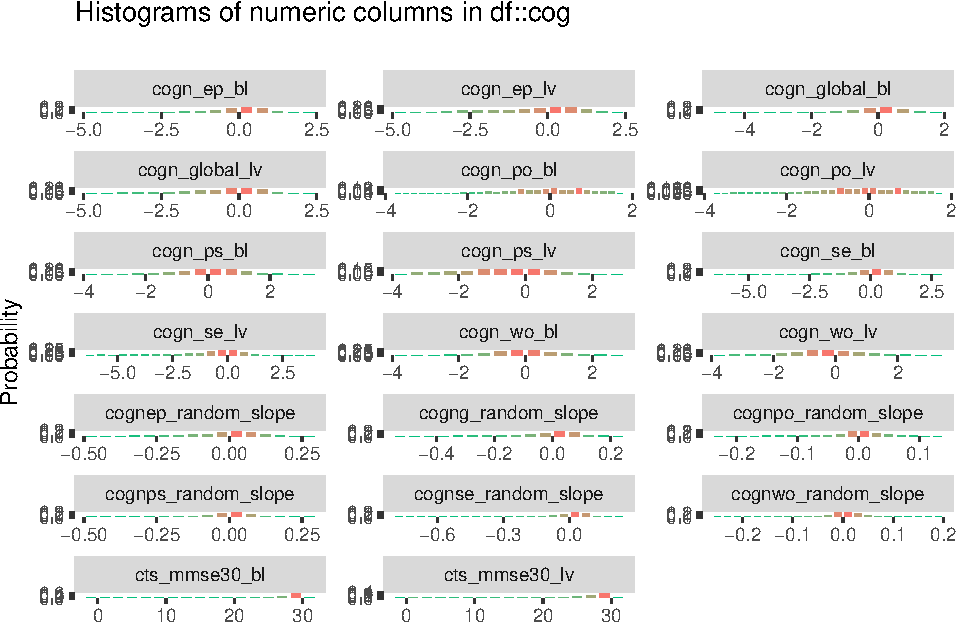
\includegraphics{notebook_files/figure-latex/unnamed-chunk-9-1.pdf}

\hypertarget{blood-measures}{%
\section{Blood Measures}\label{blood-measures}}

\begin{itemize}
\tightlist
\item
  Inflammatory markers

  \begin{itemize}
  \tightlist
  \item
    \href{https://www.radc.rush.edu/docs/var/detail.htm?category=Blood+Measures\&subcategory=Inflammatory+markers\&variable=log_agereinflam}{Age-related inflammation}: \texttt{log\_agereinflam} is a composite measure of inflammation based on levels of interleukin-1β, tumor necrosis factor-α, and interleukin-6 measured from blood samples. Only avaliable in MAP.
  \item
    \href{https://www.radc.rush.edu/docs/var/detail.htm?category=Blood+Measures\&subcategory=Inflammatory+markers\&variable=log_hil6_log_hil10}{Ratio of good to bad inflammation}: \texttt{log\_hil6\_log\_hil10} is based on levels of interleukin-6 (IL-6) and interleukin-10(IL-10) measured from blood samples.
  \end{itemize}
\item
  Routine Lab tests

  \begin{itemize}
  \tightlist
  \item
    \href{https://www.radc.rush.edu/docs/var/detail.htm?category=Blood+Measures\&subcategory=Routine+laboratory+tests\&variable=platelet}{Platelet (thrombocyte) count}: \texttt{platelet}
  \item
    \href{https://www.radc.rush.edu/docs/var/detail.htm?category=Blood+Measures\&subcategory=Routine+laboratory+tests\&variable=rbc}{Red blood cell (RBC) count}: \texttt{rbc}
  \item
    \href{https://www.radc.rush.edu/docs/var/detail.htm?category=Blood+Measures\&subcategory=Routine+laboratory+tests\&variable=rdw}{Red blood cell distribution width (RDW)}: \texttt{rdw} is a measure of the range of variation of red blood cell volume.
  \item
    \href{https://www.radc.rush.edu/docs/var/detail.htm?category=Blood+Measures\&subcategory=Routine+laboratory+tests\&variable=wbc}{White blood cell count}: \texttt{wbc}
  \end{itemize}
\end{itemize}

\hypertarget{htmlwidget-c5674fe3b0da62c2e0f0}{}
\begin{datatables}

\end{datatables}

\hypertarget{plots-7}{%
\subsection{Plots}\label{plots-7}}

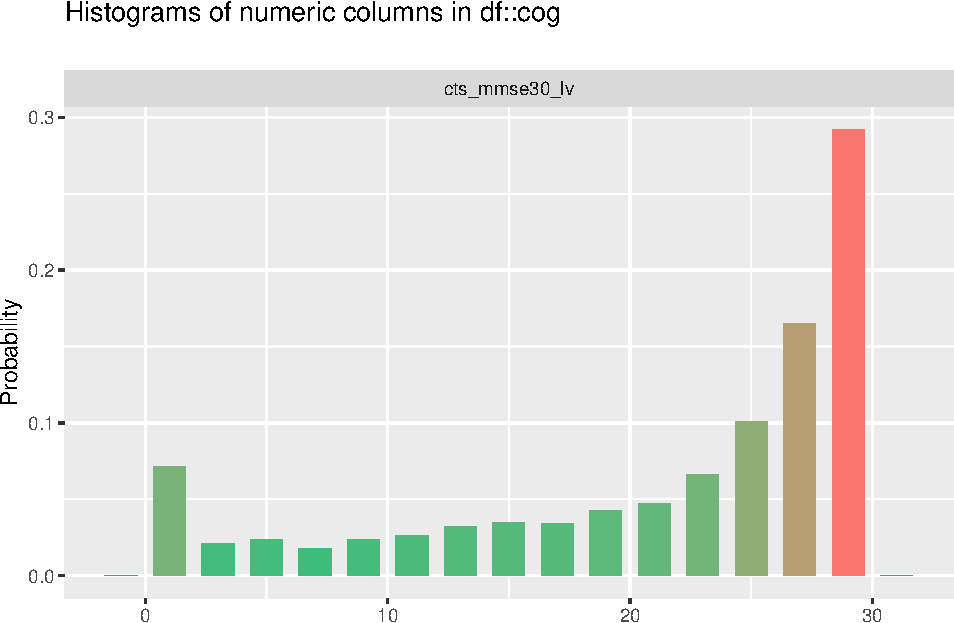
\includegraphics{notebook_files/figure-latex/unnamed-chunk-10-1.pdf}

\hypertarget{neuroimaging}{%
\section{Neuroimaging}\label{neuroimaging}}

Only 728 particpants have a MRI measurement, with only 21 also haveing a mtDNAcn measurement.

\begin{Shaded}
\begin{Highlighting}[]
\NormalTok{neuroi <-}\StringTok{ }\NormalTok{rosmap }\OperatorTok
\StringTok{  }\KeywordTok{select}\NormalTok{(study, projid, mri_id, visit, csf, gm, wm, icv,}
\NormalTok{         apoe_genotype, mtcn_avg, organ, Source.Tissue.Type, }
\NormalTok{         msex, pmi, age_bl, age_death, ad_reagan, apoe, cogdx, fu_year_lv) }
\end{Highlighting}
\end{Shaded}

\hypertarget{htmlwidget-2f7dab74f81572a99100}{}
\begin{datatables}

\end{datatables}

\hypertarget{plots-8}{%
\subsection{Plots}\label{plots-8}}

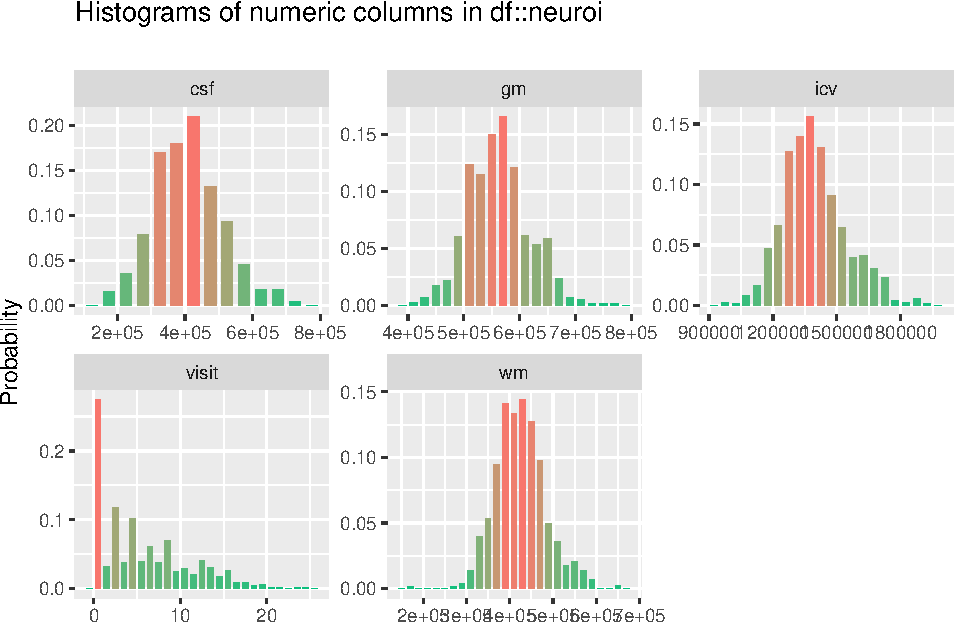
\includegraphics{notebook_files/figure-latex/unnamed-chunk-12-1.pdf}

\begin{Shaded}
\begin{Highlighting}[]
\NormalTok{rosmap }\OperatorTok
\StringTok{  }\KeywordTok{mutate}\NormalTok{(}\DataTypeTok{ad_reagan =} \KeywordTok{as_factor}\NormalTok{(ad_reagan)) }\OperatorTok
\StringTok{  }\KeywordTok{ggplot}\NormalTok{(., }\KeywordTok{aes}\NormalTok{(}\DataTypeTok{x =}\NormalTok{ ad_reagan, }\DataTypeTok{y =}\NormalTok{ icv, }\DataTypeTok{colour =}\NormalTok{ ad_reagan)) }\OperatorTok{+}\StringTok{ }
\StringTok{    }\NormalTok{ggbeeswarm}\OperatorTok{::}\KeywordTok{geom_quasirandom}\NormalTok{(}\DataTypeTok{dodge.width=}\DecValTok{1}\NormalTok{) }\OperatorTok{+}
\StringTok{ }\KeywordTok{facet_grid}\NormalTok{(. }\OperatorTok{~}\StringTok{ }\NormalTok{msex) }\OperatorTok{+}\StringTok{ }
\StringTok{  }\KeywordTok{theme_bw}\NormalTok{()}
\end{Highlighting}
\end{Shaded}

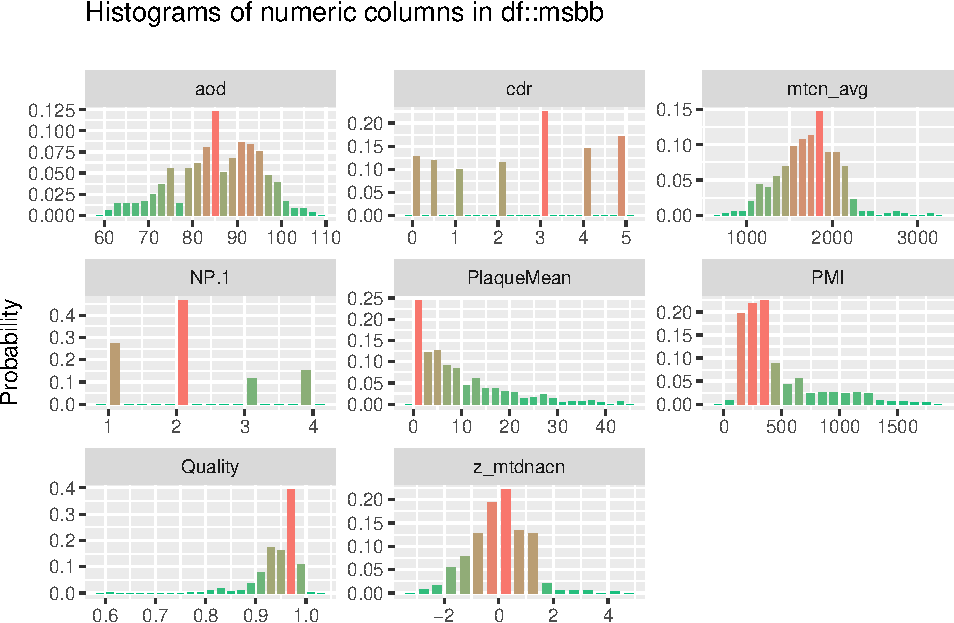
\includegraphics{notebook_files/figure-latex/unnamed-chunk-13-1.pdf}

\begin{Shaded}
\begin{Highlighting}[]
\NormalTok{rosmap }\OperatorTok
\StringTok{    }\KeywordTok{filter}\NormalTok{(}\OperatorTok{!}\KeywordTok{is.na}\NormalTok{(mtcn_avg), }\OperatorTok{!}\KeywordTok{is.na}\NormalTok{(icv)) }\OperatorTok
\StringTok{    }\KeywordTok{mutate}\NormalTok{(}\DataTypeTok{ad_reagan =} \KeywordTok{as_factor}\NormalTok{(ad_reagan), }
           \DataTypeTok{Source.Tissue.Type =} \KeywordTok{fct_drop}\NormalTok{(Source.Tissue.Type)) }\OperatorTok
\StringTok{  }\KeywordTok{ggplot}\NormalTok{(., }\KeywordTok{aes}\NormalTok{(}\DataTypeTok{x =}\NormalTok{  mtcn_avg, }\DataTypeTok{y =}\NormalTok{ icv, }\DataTypeTok{colour =}\NormalTok{ ad_reagan)) }\OperatorTok{+}\StringTok{ }
\StringTok{    }\KeywordTok{geom_point}\NormalTok{() }\OperatorTok{+}\StringTok{ }
\StringTok{    }\KeywordTok{facet_grid}\NormalTok{(Source.Tissue.Type }\OperatorTok{~}\StringTok{ }\NormalTok{msex) }\OperatorTok{+}\StringTok{ }
\StringTok{    }\KeywordTok{theme_bw}\NormalTok{()}
\end{Highlighting}
\end{Shaded}

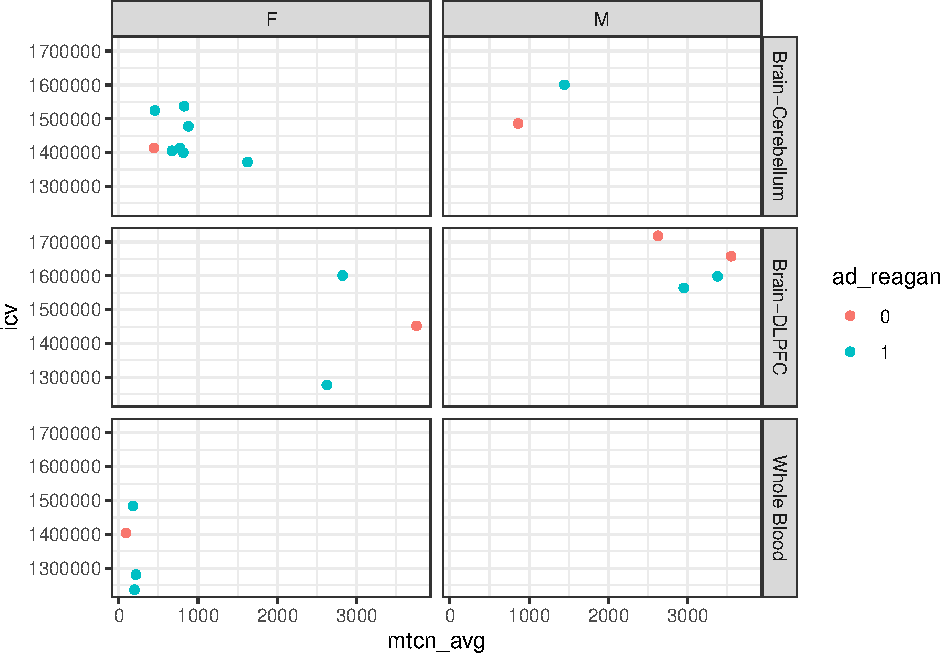
\includegraphics{notebook_files/figure-latex/unnamed-chunk-13-2.pdf}

\hypertarget{msbb}{%
\chapter{MSBB}\label{msbb}}

Samples come from 364 postmortem control, mild cognitive impaired (MCI) and AD brains with rich clinical and pathophysiological data from the Mount Sinai/JJ Peters VA Medical Center Brain Bank (MSBB--Mount Sinai NIH Neurobiobank) cohort. The majority (301) of the samples were of European ancestry, while 36 were African American, 25 were Latino, one was Asian, and one was unknown for race. Neuropathological assessments were performed using CERAD scores and Braak Staging. The CDR scale was conducted for assessment of dementia and cognitive status (\citet{10.1038/sdata.2018.185}).

Clinical Code Book: \href{https://adknowledgeportal.synapse.org/Explore/Studies?Study=syn3159438}{Synapse}

\begin{Shaded}
\begin{Highlighting}[]
\CommentTok{## MSBB}
\NormalTok{msbb.raw1 <-}\StringTok{ }\KeywordTok{read_tsv}\NormalTok{(}\StringTok{'data/AMPAD/msbb/WGS_Metadata.txt'}\NormalTok{) }
\NormalTok{msbb.raw2 <-}\StringTok{ }\KeywordTok{read_tsv}\NormalTok{(}\StringTok{'data/AMPAD_extra/msbb.wgs.meta.tsv'}\NormalTok{)}
\NormalTok{msbb.path <-}\StringTok{ }\NormalTok{readxl}\OperatorTok{::}\KeywordTok{read_xlsx}\NormalTok{(}\StringTok{'data/AMPAD_extra/msbb/TempAmp_AD-Shea-2-2020.xlsx'}\NormalTok{, }\DataTypeTok{sheet =} \DecValTok{2}\NormalTok{) }\OperatorTok\StringTok{ }
\StringTok{  }\KeywordTok{mutate}\NormalTok{(}\DataTypeTok{id =} \KeywordTok{as.character}\NormalTok{(id))}
\NormalTok{msbb.raw <-}\StringTok{ }\NormalTok{msbb.raw1 }\OperatorTok\StringTok{ }
\StringTok{  }\KeywordTok{select}\NormalTok{(WGS, individualIdentifier, PMI, RACE, CDR, SEX, NP}\FloatTok{.1}\NormalTok{, PlaqueMean, bbscore) }\OperatorTok
\StringTok{  }\KeywordTok{left_join}\NormalTok{(}\KeywordTok{select}\NormalTok{(msbb.raw2, Libid, AOD, APOE_inferred), }\DataTypeTok{by =} \KeywordTok{c}\NormalTok{(}\StringTok{'WGS'}\NormalTok{ =}\StringTok{ 'Libid'}\NormalTok{)) }\OperatorTok\StringTok{ }
\StringTok{  }\KeywordTok{mutate}\NormalTok{(}\DataTypeTok{SubNum =} \KeywordTok{str_extract}\NormalTok{(}\KeywordTok{gsub}\NormalTok{(}\StringTok{"(?<![0-9])0+"}\NormalTok{, }\StringTok{""}\NormalTok{, individualIdentifier, }\DataTypeTok{perl =} \OtherTok{TRUE}\NormalTok{), }\StringTok{'[:digit:].*'}\NormalTok{)) }\OperatorTok\StringTok{ }
\StringTok{  }\KeywordTok{left_join}\NormalTok{(msbb.path, }\DataTypeTok{by =} \KeywordTok{c}\NormalTok{(}\StringTok{'SubNum'}\NormalTok{ =}\StringTok{ 'id'}\NormalTok{)) }\OperatorTok
\StringTok{  }\KeywordTok{mutate}\NormalTok{(}\DataTypeTok{study =} \StringTok{'MSBB'}\NormalTok{, }
         \DataTypeTok{WGS =} \KeywordTok{as.character}\NormalTok{(WGS))}

\NormalTok{mosdepth <-}\StringTok{ }\KeywordTok{read_tsv}\NormalTok{(}\StringTok{"data/mosdepth/mosdepth_mtDNAcn_All.txt"}\NormalTok{)}
\NormalTok{haplogrep <-}\StringTok{ }\KeywordTok{read_tsv}\NormalTok{(}\StringTok{"data/haplogrep/haplogrep_jointAll.txt"}\NormalTok{)}

\NormalTok{xcell.raw <-}\StringTok{ }\KeywordTok{read_csv}\NormalTok{(}\StringTok{"data/xcell/ampad_xCell.csv"}\NormalTok{) }
\end{Highlighting}
\end{Shaded}

\begin{Shaded}
\begin{Highlighting}[]
\CommentTok{## Wrangle xcell data}
\NormalTok{xcell <-}\StringTok{ }\NormalTok{xcell.raw }\OperatorTok\StringTok{ }
\StringTok{  }\KeywordTok{filter}\NormalTok{(study }\OperatorTok{==}\StringTok{ "MSBB"}\NormalTok{) }\OperatorTok\StringTok{ }
\StringTok{  }\KeywordTok{group_by}\NormalTok{(Tissue, ID) }\OperatorTok\StringTok{ }
\StringTok{  }\KeywordTok{slice}\NormalTok{(}\KeywordTok{which.max}\NormalTok{(}\KeywordTok{str_length}\NormalTok{(SampleID))) }\OperatorTok\StringTok{ }
\StringTok{  }\KeywordTok{ungroup}\NormalTok{() }\OperatorTok\StringTok{ }
\StringTok{  }\KeywordTok{select}\NormalTok{(}\OperatorTok{-}\NormalTok{SampleID, }\OperatorTok{-}\NormalTok{study, }\OperatorTok{-}\NormalTok{Neurons.pval, }\OperatorTok{-}\NormalTok{Astrocytes.pval) }\OperatorTok\StringTok{ }
\StringTok{  }\KeywordTok{rename}\NormalTok{(}\DataTypeTok{rna_seq_tissue =}\NormalTok{ Tissue, }\DataTypeTok{rna_seq_batch =}\NormalTok{ batch) }\OperatorTok\StringTok{ }
\StringTok{  }\KeywordTok{pivot_wider}\NormalTok{(}\DataTypeTok{names_from =}\NormalTok{ rna_seq_tissue, }\DataTypeTok{values_from =} \KeywordTok{c}\NormalTok{(Neurons, Astrocytes, rna_seq_batch, RIN))}

\CommentTok{## Recode NP.1 -> ceradsc to be consistent with ROSMAP}
\NormalTok{msbb <-}\StringTok{ }\NormalTok{msbb.raw }\OperatorTok
\StringTok{  }\KeywordTok{left_join}\NormalTok{(haplogrep, }\DataTypeTok{by =} \KeywordTok{c}\NormalTok{(}\StringTok{'WGS'}\NormalTok{ =}\StringTok{ 'SampleID'}\NormalTok{)) }\OperatorTok
\StringTok{  }\KeywordTok{left_join}\NormalTok{(mosdepth, }\DataTypeTok{by =} \KeywordTok{c}\NormalTok{(}\StringTok{'WGS'}\NormalTok{ =}\StringTok{ 'SampleID'}\NormalTok{)) }\OperatorTok
\StringTok{  }\KeywordTok{left_join}\NormalTok{(xcell, }\DataTypeTok{by =} \KeywordTok{c}\NormalTok{(}\StringTok{"individualIdentifier"}\NormalTok{ =}\StringTok{ "ID"}\NormalTok{)) }\OperatorTok
\StringTok{  }\KeywordTok{mutate}\NormalTok{(}\DataTypeTok{id =} \KeywordTok{paste0}\NormalTok{(}\StringTok{'MSBB'}\NormalTok{, WGS)) }\OperatorTok
\StringTok{  }\KeywordTok{mutate}\NormalTok{(}\DataTypeTok{APOE_inferred =} \KeywordTok{recode}\NormalTok{(APOE_inferred, }\StringTok{'e2/e2'}\NormalTok{ =}\StringTok{ '22'}\NormalTok{, }\StringTok{'e2/e3'}\NormalTok{ =}\StringTok{ '23'}\NormalTok{, }\StringTok{'e3/e3'}\NormalTok{ =}\StringTok{ '33'}\NormalTok{, }\StringTok{'e2/e4'}\NormalTok{ =}\StringTok{ '24'}\NormalTok{, }\StringTok{'e3/e4'}\NormalTok{ =}\StringTok{ '34'}\NormalTok{, }\StringTok{'e4/e4'}\NormalTok{ =}\StringTok{ '44'}\NormalTok{),}
        \DataTypeTok{apoe4 =} \KeywordTok{recode}\NormalTok{(APOE_inferred, }\StringTok{'22'}\NormalTok{ =}\StringTok{ 'e4-'}\NormalTok{, }\StringTok{'23'}\NormalTok{ =}\StringTok{ 'e4-'}\NormalTok{, }\StringTok{'33'}\NormalTok{ =}\StringTok{ 'e4-'}\NormalTok{, }\StringTok{'24'}\NormalTok{ =}\StringTok{ 'e4+'}\NormalTok{, }\StringTok{'34'}\NormalTok{ =}\StringTok{ 'e4+'}\NormalTok{, }\StringTok{'44'}\NormalTok{ =}\StringTok{ 'e4+'}\NormalTok{),}
        \DataTypeTok{SEX =} \KeywordTok{as.factor}\NormalTok{(SEX),}
        \DataTypeTok{aod_cat =} \KeywordTok{cut}\NormalTok{(AOD, }\KeywordTok{c}\NormalTok{(}\DecValTok{50}\NormalTok{, }\DecValTok{60}\NormalTok{, }\DecValTok{70}\NormalTok{, }\DecValTok{80}\NormalTok{, }\DecValTok{90}\NormalTok{, }\OtherTok{Inf}\NormalTok{), }\KeywordTok{c}\NormalTok{(}\StringTok{'50-59'}\NormalTok{, }\StringTok{'60-69'}\NormalTok{, }\StringTok{'70-79'}\NormalTok{, }\StringTok{'80-89'}\NormalTok{, }\StringTok{'90+'}\NormalTok{), }\DataTypeTok{right =} \OtherTok{FALSE}\NormalTok{),}
        \DataTypeTok{aod_cat =} \KeywordTok{ordered}\NormalTok{(aod_cat, }\DataTypeTok{levels =} \KeywordTok{c}\NormalTok{(}\StringTok{'50-59'}\NormalTok{, }\StringTok{'60-69'}\NormalTok{, }\StringTok{'70-79'}\NormalTok{, }\StringTok{'80-89'}\NormalTok{, }\StringTok{'90+'}\NormalTok{)), }
        \DataTypeTok{SourceTissue =} \StringTok{'prefrontal cortex'}\NormalTok{,}
        \DataTypeTok{APOE_inferred =} \KeywordTok{as.factor}\NormalTok{(APOE_inferred), }
        \DataTypeTok{apoe4 =} \KeywordTok{as.factor}\NormalTok{(apoe4), }
        \DataTypeTok{RACE =} \KeywordTok{as.factor}\NormalTok{(RACE), }
        \DataTypeTok{z_mtdnacn =} \KeywordTok{scale}\NormalTok{(mtcn_avg, }\DataTypeTok{center =} \OtherTok{TRUE}\NormalTok{, }\DataTypeTok{scale =} \OtherTok{TRUE}\NormalTok{)[,}\DecValTok{1}\NormalTok{],}
        \DataTypeTok{macro =} \KeywordTok{case_when}\NormalTok{(}
          \KeywordTok{str_detect}\NormalTok{(Haplogroup, }\StringTok{"^L|^HV|^JT"}\NormalTok{) }\OperatorTok{~}\StringTok{ }\KeywordTok{substr}\NormalTok{(Haplogroup, }\DataTypeTok{start =} \DecValTok{1}\NormalTok{, }\DataTypeTok{stop =} \DecValTok{2}\NormalTok{),}
                     \OtherTok{TRUE} \OperatorTok{~}\StringTok{ }\KeywordTok{substr}\NormalTok{(Haplogroup, }\DataTypeTok{start =} \DecValTok{1}\NormalTok{, }\DataTypeTok{stop =} \DecValTok{1}\NormalTok{)),}
        \DataTypeTok{cerad =} \KeywordTok{recode}\NormalTok{(NP}\FloatTok{.1}\NormalTok{, }\StringTok{'1'}\NormalTok{ =}\StringTok{ 'Normal'}\NormalTok{, }\StringTok{'2'}\NormalTok{ =}\StringTok{ 'Definite'}\NormalTok{, }\StringTok{'3'}\NormalTok{ =}\StringTok{ 'Probable'}\NormalTok{, }\StringTok{'4'}\NormalTok{ =}\StringTok{ 'Possible'}\NormalTok{),}
        \DataTypeTok{cerad =} \KeywordTok{ordered}\NormalTok{(cerad, }\DataTypeTok{levels =} \KeywordTok{c}\NormalTok{(}\StringTok{'Normal'}\NormalTok{, }\StringTok{'Possible'}\NormalTok{, }\StringTok{'Probable'}\NormalTok{, }\StringTok{'Definite'}\NormalTok{)),}
        \DataTypeTok{ceradsc =} \KeywordTok{pmax}\NormalTok{(HippoPlaquesWCoresValue, EntorPlaquesWCoresValue, MidPlaquesWCoresValue, }
\NormalTok{                       SupPlaquesWCoresValue, InfPlaquesWCoresValue, OcciPlaquesWCoresValue),}
        \DataTypeTok{ceradsc =} \KeywordTok{ordered}\NormalTok{(ceradsc),}
        \DataTypeTok{ceradsc =} \KeywordTok{fct_recode}\NormalTok{(ceradsc, }\StringTok{'4'}\NormalTok{ =}\StringTok{ '0'}\NormalTok{, }\StringTok{'3'}\NormalTok{ =}\StringTok{ '1'}\NormalTok{, }\StringTok{'2'}\NormalTok{ =}\StringTok{ '3'}\NormalTok{, }\StringTok{'1'}\NormalTok{ =}\StringTok{ '5'}\NormalTok{),}
        \DataTypeTok{bbscore =} \KeywordTok{ordered}\NormalTok{(bbscore, }\DataTypeTok{levels =} \KeywordTok{c}\NormalTok{(}\StringTok{'0'}\NormalTok{, }\StringTok{'1'}\NormalTok{, }\StringTok{'2'}\NormalTok{, }\StringTok{'3'}\NormalTok{, }\StringTok{'4'}\NormalTok{, }\StringTok{'5'}\NormalTok{, }\StringTok{'6'}\NormalTok{)),}
        \DataTypeTok{niareagansc =} \KeywordTok{case_when}\NormalTok{(}
\NormalTok{          ceradsc }\OperatorTok{==}\StringTok{ }\DecValTok{4} \OperatorTok{&}\StringTok{ }\NormalTok{bbscore }\OperatorTok{==}\StringTok{ }\DecValTok{0} \OperatorTok{~}\StringTok{ }\DecValTok{4}\NormalTok{, }
\NormalTok{          ceradsc }\OperatorTok{==}\StringTok{ }\DecValTok{4} \OperatorTok{&}\StringTok{ }\NormalTok{bbscore }\OperatorTok\StringTok{ }\KeywordTok{c}\NormalTok{(}\DecValTok{1}\OperatorTok{:}\DecValTok{6}\NormalTok{) }\OperatorTok{~}\StringTok{ }\DecValTok{3}\NormalTok{, }
\NormalTok{          ceradsc }\OperatorTok{==}\StringTok{ }\DecValTok{3} \OperatorTok{&}\StringTok{ }\NormalTok{bbscore }\OperatorTok\StringTok{ }\KeywordTok{c}\NormalTok{(}\DecValTok{0}\OperatorTok{:}\DecValTok{6}\NormalTok{) }\OperatorTok{~}\StringTok{ }\DecValTok{3}\NormalTok{, }
\NormalTok{          ceradsc }\OperatorTok{==}\StringTok{ }\DecValTok{2} \OperatorTok{&}\StringTok{ }\NormalTok{bbscore }\OperatorTok\StringTok{ }\KeywordTok{c}\NormalTok{(}\DecValTok{0}\OperatorTok{:}\DecValTok{2}\NormalTok{) }\OperatorTok{~}\StringTok{ }\DecValTok{3}\NormalTok{,}
\NormalTok{          ceradsc }\OperatorTok{==}\StringTok{ }\DecValTok{2} \OperatorTok{&}\StringTok{ }\NormalTok{bbscore }\OperatorTok\StringTok{ }\KeywordTok{c}\NormalTok{(}\DecValTok{3}\OperatorTok{:}\DecValTok{6}\NormalTok{) }\OperatorTok{~}\StringTok{ }\DecValTok{2}\NormalTok{,}
\NormalTok{          ceradsc }\OperatorTok{==}\StringTok{ }\DecValTok{1} \OperatorTok{&}\StringTok{ }\NormalTok{bbscore }\OperatorTok\StringTok{ }\KeywordTok{c}\NormalTok{(}\DecValTok{0}\OperatorTok{:}\DecValTok{4}\NormalTok{) }\OperatorTok{~}\StringTok{ }\DecValTok{2}\NormalTok{,}
\NormalTok{          ceradsc }\OperatorTok{==}\StringTok{ }\DecValTok{1} \OperatorTok{&}\StringTok{ }\NormalTok{bbscore }\OperatorTok\StringTok{ }\KeywordTok{c}\NormalTok{(}\DecValTok{5}\OperatorTok{:}\DecValTok{6}\NormalTok{) }\OperatorTok{~}\StringTok{ }\DecValTok{1}\NormalTok{,}
\NormalTok{        ), }
        \DataTypeTok{niareagansc =} \KeywordTok{ordered}\NormalTok{(niareagansc, }\DataTypeTok{levels =} \KeywordTok{c}\NormalTok{(}\StringTok{'4'}\NormalTok{, }\StringTok{'3'}\NormalTok{, }\StringTok{'2'}\NormalTok{, }\StringTok{'1'}\NormalTok{)),}
        \DataTypeTok{ad_reagan =} \KeywordTok{fct_recode}\NormalTok{(niareagansc, }\StringTok{"1"}\NormalTok{ =}\StringTok{ "1"}\NormalTok{, }\StringTok{"1"}\NormalTok{ =}\StringTok{ "2"}\NormalTok{, }\StringTok{"0"}\NormalTok{ =}\StringTok{ "3"}\NormalTok{, }\StringTok{"0"}\NormalTok{ =}\StringTok{ "4"}\NormalTok{),}
        \DataTypeTok{braaksc_B =} \KeywordTok{fct_recode}\NormalTok{(bbscore, }\DataTypeTok{B0 =} \StringTok{"0"}\NormalTok{, }\DataTypeTok{B1 =} \StringTok{"1"}\NormalTok{, }\DataTypeTok{B1 =} \StringTok{"2"}\NormalTok{, }\DataTypeTok{B2 =} \StringTok{"3"}\NormalTok{, }\DataTypeTok{B2 =} \StringTok{"4"}\NormalTok{, }\DataTypeTok{B3 =} \StringTok{"5"}\NormalTok{, }\DataTypeTok{B3 =} \StringTok{"6"}\NormalTok{), }
        \DataTypeTok{ceradsc_C =} \KeywordTok{fct_recode}\NormalTok{(ceradsc, }\DataTypeTok{C0 =} \StringTok{"1"}\NormalTok{, }\DataTypeTok{C1 =} \StringTok{"2"}\NormalTok{, }\DataTypeTok{C2 =} \StringTok{"3"}\NormalTok{, }\DataTypeTok{C3 =} \StringTok{"4"}\NormalTok{)) }\OperatorTok
\StringTok{  }\KeywordTok{mutate_at}\NormalTok{(}\KeywordTok{vars}\NormalTok{(HippoPlaquesWCoresValue, EntorPlaquesWCoresValue, MidPlaquesWCoresValue, }
\NormalTok{                       SupPlaquesWCoresValue, InfPlaquesWCoresValue, OcciPlaquesWCoresValue), }
\NormalTok{            ordered) }\OperatorTok
\StringTok{  }\KeywordTok{select}\NormalTok{(id, individualIdentifier, study, }\DataTypeTok{sex =}\NormalTok{ SEX, }\DataTypeTok{race =}\NormalTok{ RACE, SourceTissue, }
\NormalTok{         PMI, NP}\FloatTok{.1}\NormalTok{, cerad, niareagansc, ad_reagan, ceradsc, HippoPlaquesWCoresValue, }
\NormalTok{         EntorPlaquesWCoresValue, MidPlaquesWCoresValue, SupPlaquesWCoresValue, }
\NormalTok{         InfPlaquesWCoresValue, OcciPlaquesWCoresValue, }\DataTypeTok{braaksc =}\NormalTok{ bbscore, braaksc_B, }
\NormalTok{         ceradsc_C, }\DataTypeTok{apoe =}\NormalTok{ APOE_inferred, apoe4, }\DataTypeTok{aod =}\NormalTok{ AOD, aod_cat, }\DataTypeTok{cdr =}\NormalTok{ CDR, }
\NormalTok{         PlaqueMean, mtcn_avg, z_mtdnacn, Haplogroup, Quality, macro, }
\NormalTok{         Neurons_BM10, Neurons_BM22, Neurons_BM36, Neurons_BM44, }
\NormalTok{         Astrocytes_BM10, Astrocytes_BM22, Astrocytes_BM36, Astrocytes_BM44, }
\NormalTok{         rna_seq_batch_BM10, rna_seq_batch_BM22, rna_seq_batch_BM36, rna_seq_batch_BM44, }
\NormalTok{         RIN_BM10, RIN_BM22, RIN_BM36, RIN_BM44)}

\KeywordTok{write_rds}\NormalTok{(msbb, }\StringTok{'output/msbb.rds'}\NormalTok{)}
\end{Highlighting}
\end{Shaded}

\hypertarget{msbb-pathology}{%
\section{MSBB Pathology}\label{msbb-pathology}}

\textbf{Amyloid}

\begin{itemize}
\tightlist
\item
  \texttt{HippoPlaquesWCoresValue}, \texttt{EntorPlaquesWCoresValue}, \texttt{MidPlaquesWCoresValue}, \texttt{SupPlaquesWCoresValue}, \texttt{InfPlaquesWCoresValue}, \texttt{OcciPlaquesWCoresValue}: Neuritic plaque burden measured in 8 brain regions. (0 = Absent; 1 = Sparese; 3 = Moderate; 5 = Frequent)

  \begin{itemize}
  \tightlist
  \item
    requested from Haroutunian, Vahram on March 4 2020
  \end{itemize}
\item
  \texttt{ceradsc}: semiquantitative estimates of neuritic plaque density modified to be implemented without adjustment for age and clinical diagnosis, as implemented in \href{https://www.radc.rush.edu/docs/var/detail.htm?category=Pathology\&subcategory=Alzheimer\%27s+disease\&variable=ceradsc}{ROSMAP}
\item
  score is derived from the brain region with the greatest number of neuritic plaques
\item
  \texttt{PlaqueMean}: Average number of plaques across brain regions
\end{itemize}

\textbf{Nurofibilary Tangles}

\begin{itemize}
\tightlist
\item
  \texttt{braaksc}: Braak Stage is a semiquantitative measure of severity of neurofibrillary tangle (NFT) pathology
\end{itemize}

\textbf{Neuropathological Diagnosis}

\begin{itemize}
\tightlist
\item
  \texttt{cerad}/\texttt{NP.1}: Neuropathology Category as measured by CERAD (1=Normal, 2=Definite AD, 3=probable AD, 4=possible AD)
\item
  \texttt{niareagansc}: modified NIA-Reagan diagnosis of Alzheimer's disease is based on consensus recommendations for postmortem diagnosis of Alzheimer's disease. The criteria rely on both neurofibrillary tangles (Braak) and neuritic plaques (CERAD) and does not account for clinical information.

  \begin{itemize}
  \tightlist
  \item
    1 = High; 2 = Intermediate; 3 = Low; 4 = No AD
  \item
    Implemented to match coding from
    \href{https://www.radc.rush.edu/docs/var/detail.htm?category=Pathology\&subcategory=Alzheimer\%27s+disease\&variable=niareagansc}{ROSMAP}.\\
  \end{itemize}
\item
  \texttt{ad\_reagan}: dichotomized NIA-Reagan diagnosis
\end{itemize}

\label{tab:msbb-path-numeric}Variable type: Numeric

col\_name

min

q1

median

mean

q3

max

sd

pcnt\_na

PlaqueMean

0

1.68

6.51

9.01

13.2

43.84

9.21

0

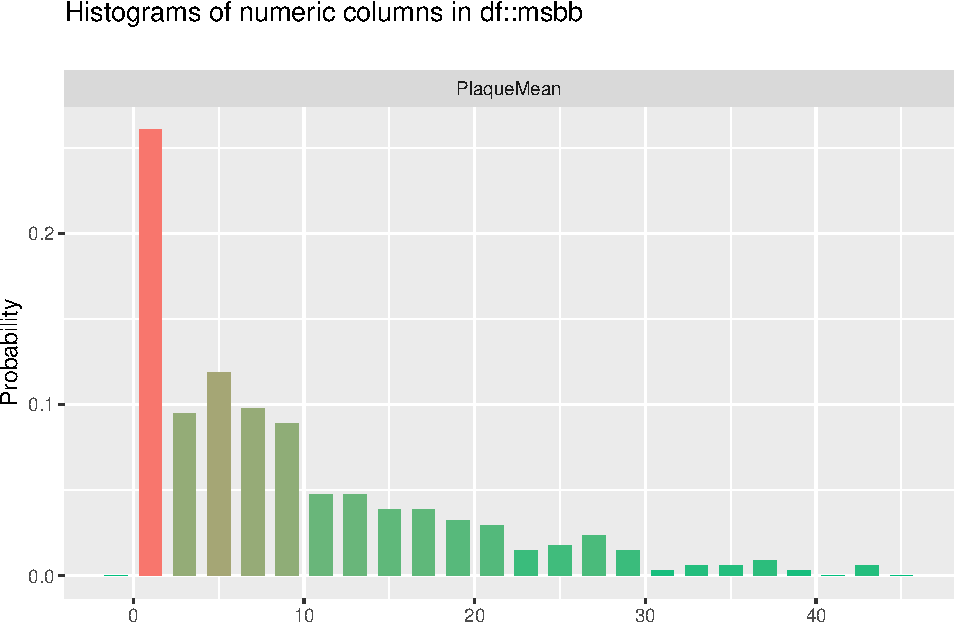
\includegraphics{notebook_files/figure-latex/msbb-path-n-plot-1.pdf}

\hypertarget{htmlwidget-1457c581883989f1fb1a}{}
\begin{datatables}

\end{datatables}

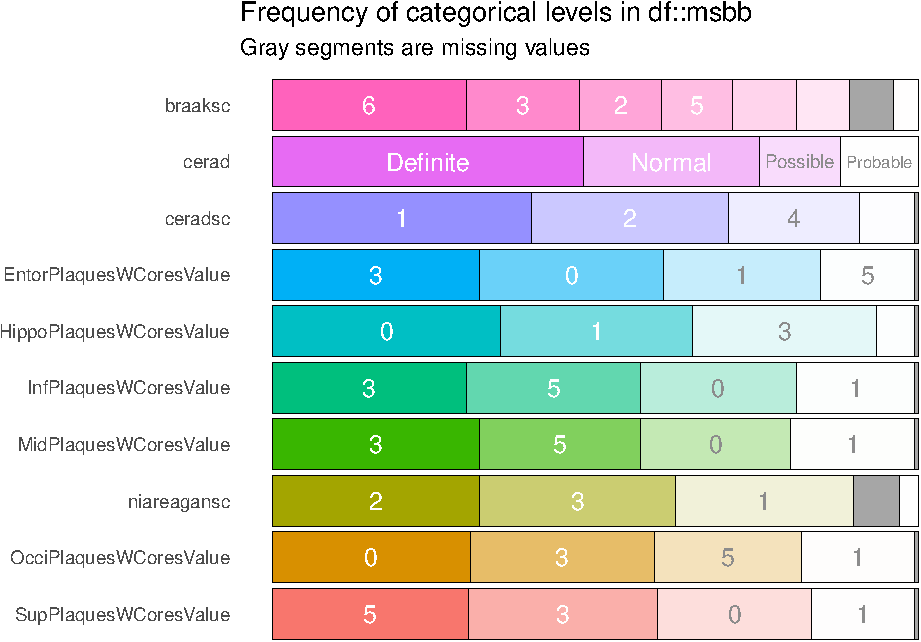
\includegraphics{notebook_files/figure-latex/msbb-path-c-plot-1.pdf}

\hypertarget{cross-tabs}{%
\subsection{Cross-tabs}\label{cross-tabs}}

\textbf{Characteristic}

0

1

2

3

4

5

6

Unknown

\textbf{Total}

\textbf{ceradsc}

4

10 (3.0\%)

16 (4.7\%)

22 (6.5\%)

16 (4.7\%)

2 (0.6\%)

0 (0\%)

0 (0\%)

2 (0.6\%)

68 (20\%)

3

2 (0.6\%)

2 (0.6\%)

8 (2.4\%)

10 (3.0\%)

3 (0.9\%)

1 (0.3\%)

0 (0\%)

3 (0.9\%)

29 (8.6\%)

2

1 (0.3\%)

9 (2.7\%)

10 (3.0\%)

20 (5.9\%)

11 (3.3\%)

18 (5.3\%)

26 (7.7\%)

8 (2.4\%)

103 (31\%)

1

0 (0\%)

1 (0.3\%)

3 (0.9\%)

13 (3.9\%)

16 (4.7\%)

18 (5.3\%)

75 (22\%)

9 (2.7\%)

135 (40\%)

Unknown

0 (0\%)

0 (0\%)

0 (0\%)

0 (0\%)

1 (0.3\%)

0 (0\%)

0 (0\%)

1 (0.3\%)

2 (0.6\%)

\textbf{Total}

13 (3.9\%)

28 (8.3\%)

43 (13\%)

59 (18\%)

33 (9.8\%)

37 (11\%)

101 (30\%)

23 (6.8\%)

337 (100\%)

\textbf{Characteristic}

NoAD

Low

Intermediate

High

Unknown

\textbf{Total}

\textbf{cerad}

Normal

10 (3.0\%)

72 (21\%)

3 (0.9\%)

0 (0\%)

7 (2.1\%)

92 (27\%)

Possible

0 (0\%)

20 (5.9\%)

22 (6.5\%)

0 (0\%)

0 (0\%)

42 (12\%)

Probable

0 (0\%)

6 (1.8\%)

31 (9.2\%)

0 (0\%)

4 (1.2\%)

41 (12\%)

Definite

0 (0\%)

4 (1.2\%)

52 (15\%)

93 (28\%)

13 (3.9\%)

162 (48\%)

\textbf{Total}

10 (3.0\%)

102 (30\%)

108 (32\%)

93 (28\%)

24 (7.1\%)

337 (100\%)

\hypertarget{plots}{%
\subsection{Plots}\label{plots}}

\begin{figure}
\centering
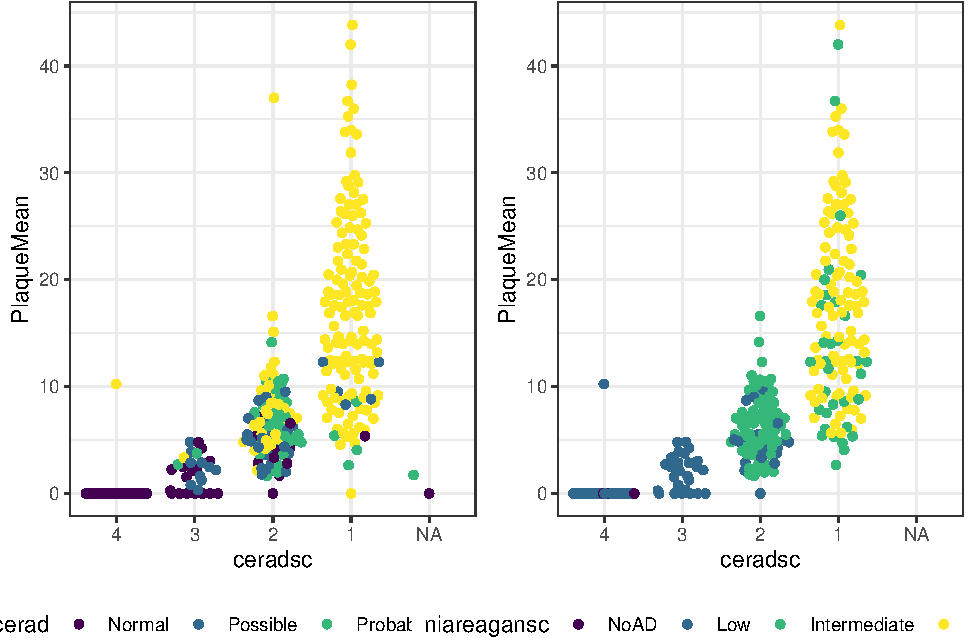
\includegraphics{notebook_files/figure-latex/msbb-plot-plq-cerad-1.pdf}
\caption{\label{fig:msbb-plot-plq-cerad}Distribution of amyloid by neuropathological diagnosis}
\end{figure}

\begin{figure}
\centering
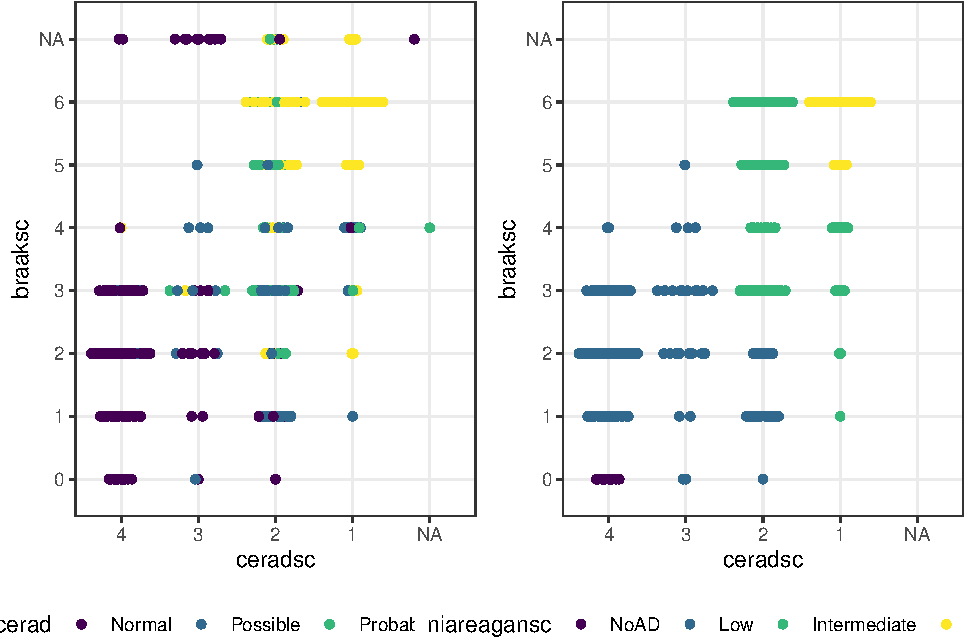
\includegraphics{notebook_files/figure-latex/msbb-plot-plq-braak-1.pdf}
\caption{\label{fig:msbb-plot-plq-braak}Distribution of neuropathological diagnosis by ceradsc and braaksc}
\end{figure}

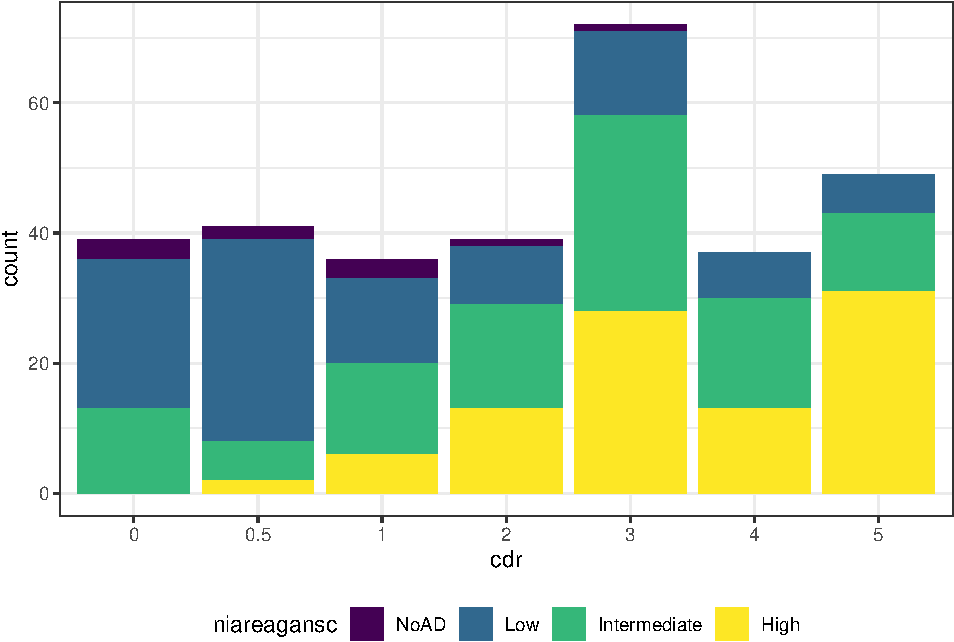
\includegraphics{notebook_files/figure-latex/msbb-plot-cdr-niareagan-1.pdf} 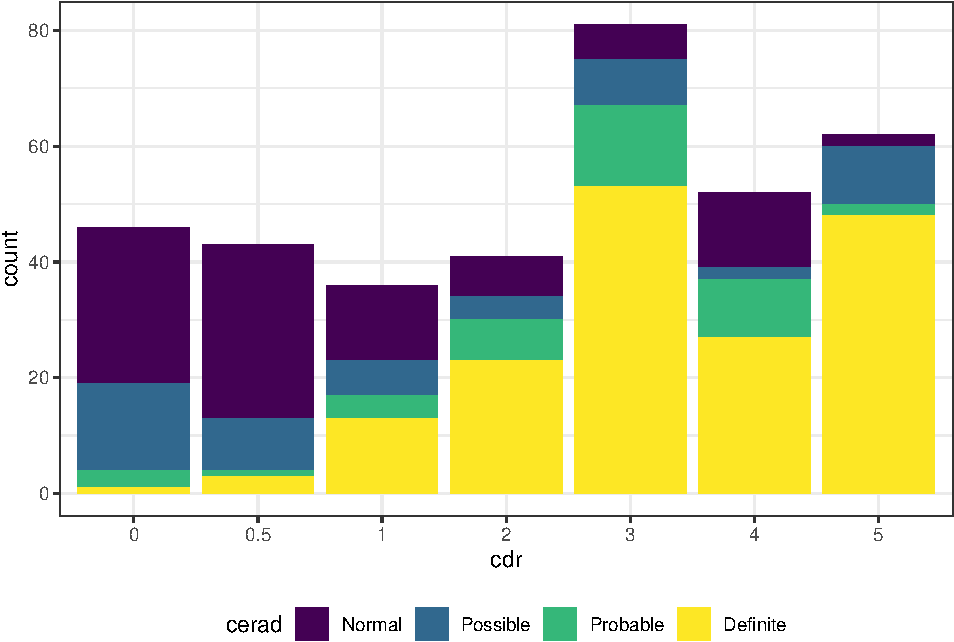
\includegraphics{notebook_files/figure-latex/msbb-plot-cdr-niareagan-2.pdf}

\begin{figure}
\centering
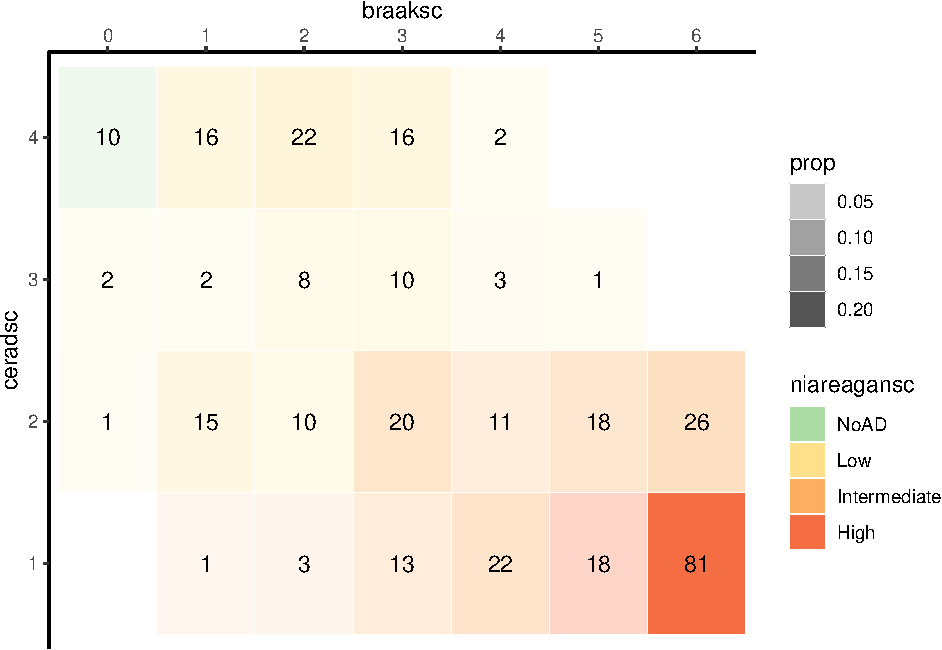
\includegraphics{notebook_files/figure-latex/msbb-plot-cerad-braak-1.pdf}
\caption{\label{fig:msbb-plot-cerad-braak}Cross-tabs of cerad \& braaksc}
\end{figure}

\hypertarget{msbb-other-variables}{%
\section{MSBB Other Variables}\label{msbb-other-variables}}

\label{tab:msbb-numeric}Variable type: Numeric

col\_name

min

q1

median

mean

q3

max

sd

pcnt\_na

PMI

75.00

220.00

315.00

445.56

550.00

1800.00

334.94

0.00

cdr

0.00

1.00

3.00

2.46

4.00

5.00

1.71

0.00

aod

61.00

79.00

85.00

84.93

92.50

108.00

9.61

0.59

mtcn\_avg

734.20

1513.48

1732.57

1720.37

1921.49

3151.59

335.96

0.00

Quality

0.67

0.90

0.93

0.92

0.95

1.00

0.04

0.00

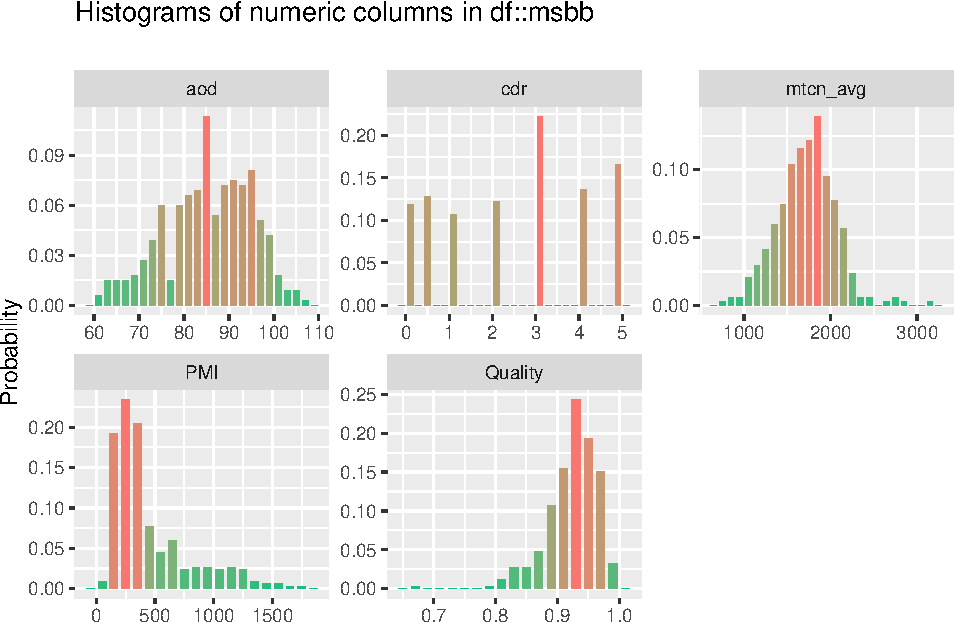
\includegraphics{notebook_files/figure-latex/unnamed-chunk-16-1.pdf}

\hypertarget{htmlwidget-85df3e376dcce9f518ab}{}
\begin{datatables}

\end{datatables}

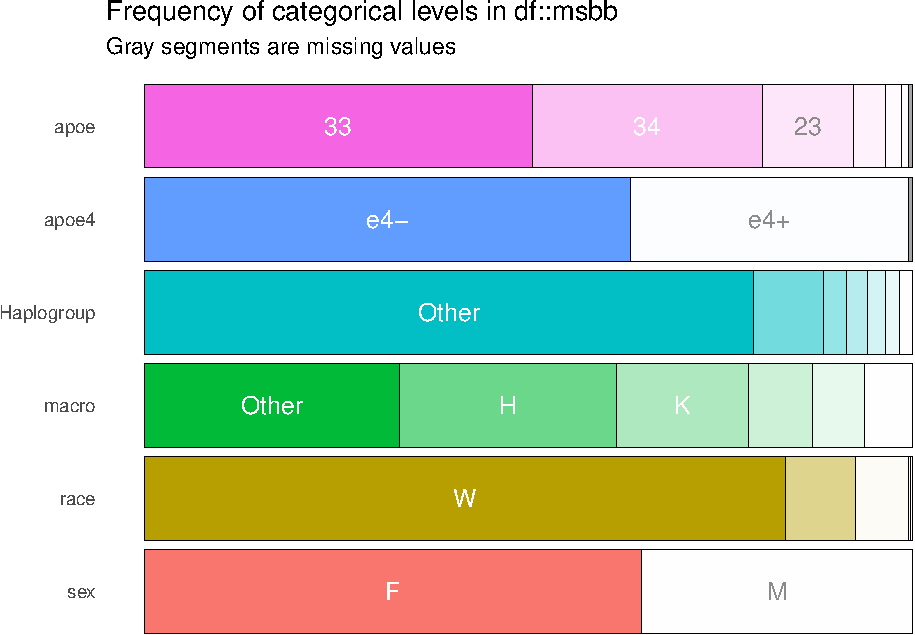
\includegraphics{notebook_files/figure-latex/unnamed-chunk-17-1.pdf}

\hypertarget{msbb-rna-seq}{%
\section{MSBB RNA-seq}\label{msbb-rna-seq}}

\begin{itemize}
\tightlist
\item
  WGS (ie mtDNAcn) was generated from DNA isolated from BM10 or BM22
\item
  RNAseq data was generated from DNA isolated from BM10, BM22, BM36 and BM44
\end{itemize}

\label{tab:msbb-rna-numeric}Variable type: Numeric

col\_name

min

q1

median

mean

q3

max

sd

pcnt\_na

Neurons\_BM10

0.01

0.06

0.07

0.06

0.08

0.09

0.02

27.60

Neurons\_BM22

0.00

0.05

0.06

0.06

0.07

0.09

0.02

33.23

Neurons\_BM36

0.00

0.04

0.06

0.06

0.07

0.09

0.02

37.09

Neurons\_BM44

0.00

0.05

0.07

0.06

0.08

0.09

0.02

35.31

Astrocytes\_BM10

0.00

0.01

0.01

0.02

0.02

0.11

0.02

27.60

Astrocytes\_BM22

0.00

0.01

0.02

0.03

0.04

0.16

0.02

33.23

Astrocytes\_BM36

0.00

0.01

0.02

0.03

0.04

0.11

0.02

37.09

Astrocytes\_BM44

0.01

0.02

0.03

0.04

0.04

0.14

0.02

35.31

RIN\_BM10

2.10

5.90

6.60

6.47

7.30

9.60

1.34

27.60

RIN\_BM22

2.20

5.20

6.00

6.06

7.00

10.00

1.25

33.23

RIN\_BM36

2.20

5.10

6.30

6.06

7.10

9.00

1.54

37.09

RIN\_BM44

2.00

5.90

7.95

7.54

9.88

10.00

2.29

35.31

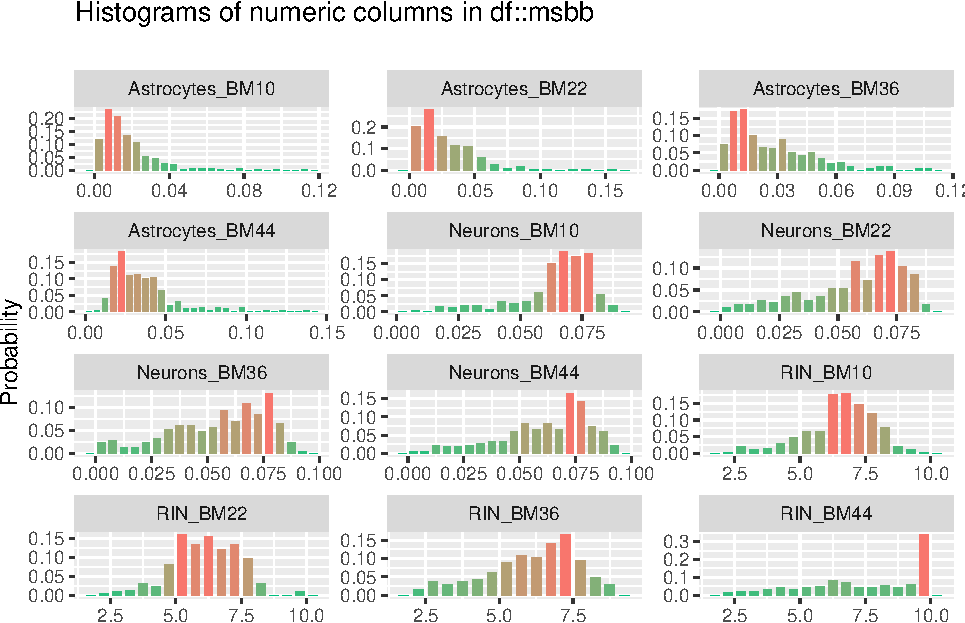
\includegraphics{notebook_files/figure-latex/msbb-rna-plot-1.pdf}

\begin{Shaded}
\begin{Highlighting}[]
\NormalTok{msbb_xcell <-}\StringTok{ }\NormalTok{xcell.raw }\OperatorTok\StringTok{ }
\StringTok{  }\KeywordTok{filter}\NormalTok{(study }\OperatorTok{==}\StringTok{ "MSBB"}\NormalTok{) }\OperatorTok
\StringTok{  }\KeywordTok{select}\NormalTok{(}\OperatorTok{-}\NormalTok{Neurons.pval, }\OperatorTok{-}\NormalTok{Astrocytes.pval, }\OperatorTok{-}\NormalTok{study) }\OperatorTok\StringTok{ }
\StringTok{  }\KeywordTok{left_join}\NormalTok{(.,}
            \KeywordTok{select}\NormalTok{(msbb, individualIdentifier, aod, ad_reagan, cdr, mtcn_avg, sex),}
            \DataTypeTok{by =} \KeywordTok{c}\NormalTok{(}\StringTok{"ID"}\NormalTok{ =}\StringTok{ "individualIdentifier"}\NormalTok{))  }\OperatorTok\StringTok{ }
\StringTok{    }\KeywordTok{pivot_longer}\NormalTok{(}\KeywordTok{c}\NormalTok{(}\StringTok{"Neurons"}\NormalTok{, }\StringTok{"Astrocytes"}\NormalTok{), }\DataTypeTok{names_to =} \StringTok{"cells"}\NormalTok{, }\DataTypeTok{values_to =} \StringTok{"xcell"}\NormalTok{)}

\KeywordTok{ggplot}\NormalTok{(msbb_xcell, }\KeywordTok{aes}\NormalTok{(}\DataTypeTok{x =}\NormalTok{ ad_reagan, }\DataTypeTok{y =}\NormalTok{ xcell, }\DataTypeTok{colour =}\NormalTok{ cells)) }\OperatorTok{+}\StringTok{ }
\StringTok{  }\NormalTok{ggbeeswarm}\OperatorTok{::}\KeywordTok{geom_quasirandom}\NormalTok{(}\DataTypeTok{dodge.width=}\DecValTok{1}\NormalTok{) }\OperatorTok{+}\StringTok{ }
\StringTok{  }\KeywordTok{facet_grid}\NormalTok{(cells }\OperatorTok{~}\StringTok{ }\NormalTok{Tissue) }\OperatorTok{+}\StringTok{ }
\StringTok{  }\KeywordTok{theme_bw}\NormalTok{()}
\end{Highlighting}
\end{Shaded}

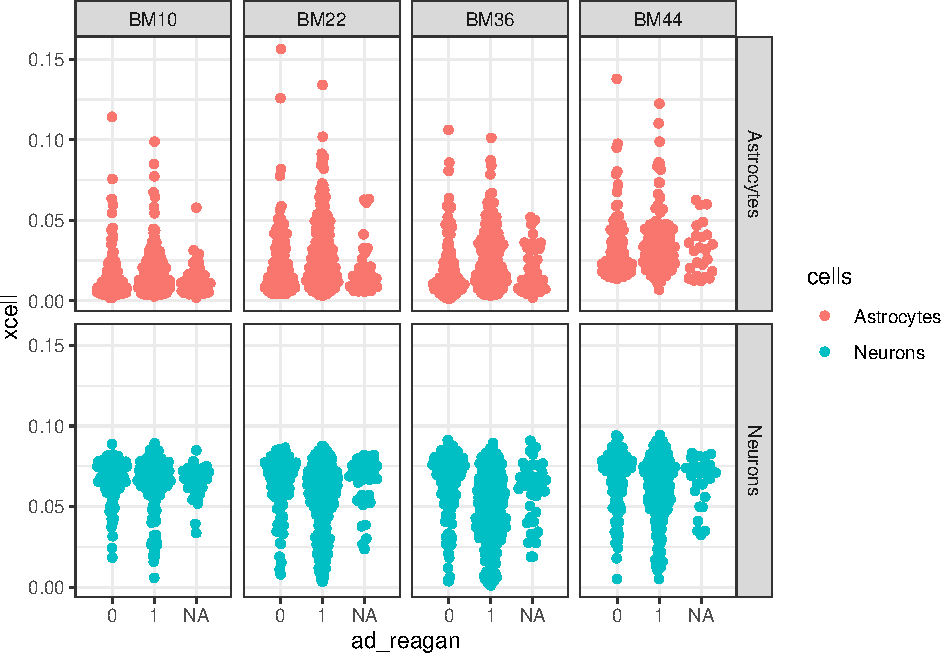
\includegraphics{notebook_files/figure-latex/msbb-rna-dx-plots-1.pdf}

\begin{Shaded}
\begin{Highlighting}[]
\KeywordTok{ggplot}\NormalTok{(msbb_xcell, }\KeywordTok{aes}\NormalTok{(}\DataTypeTok{x =}\NormalTok{ cdr, }\DataTypeTok{y =}\NormalTok{ xcell, }\DataTypeTok{colour =}\NormalTok{ cells)) }\OperatorTok{+}\StringTok{ }
\StringTok{  }\NormalTok{ggbeeswarm}\OperatorTok{::}\KeywordTok{geom_quasirandom}\NormalTok{(}\DataTypeTok{dodge.width=}\DecValTok{1}\NormalTok{) }\OperatorTok{+}\StringTok{ }
\StringTok{  }\KeywordTok{geom_smooth}\NormalTok{(}\DataTypeTok{method =}\NormalTok{ lm) }\OperatorTok{+}\StringTok{ }
\StringTok{  }\KeywordTok{facet_grid}\NormalTok{(cells }\OperatorTok{~}\StringTok{ }\NormalTok{Tissue) }\OperatorTok{+}\StringTok{ }
\StringTok{  }\KeywordTok{theme_bw}\NormalTok{()}
\end{Highlighting}
\end{Shaded}

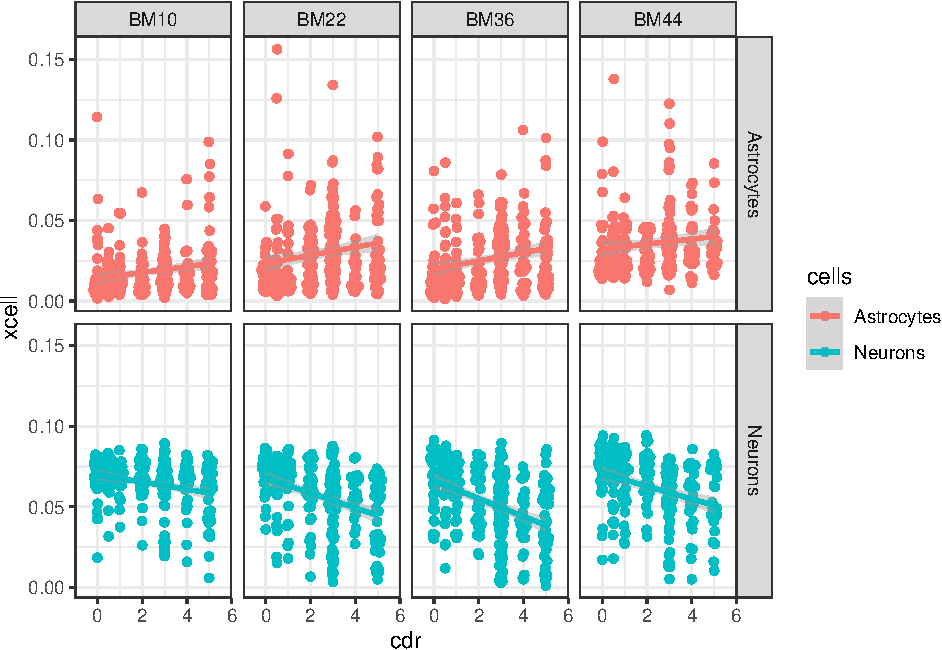
\includegraphics{notebook_files/figure-latex/msbb-rna-dx-plots-2.pdf}

\begin{Shaded}
\begin{Highlighting}[]
\KeywordTok{ggplot}\NormalTok{(msbb_xcell, }\KeywordTok{aes}\NormalTok{(}\DataTypeTok{x =}\NormalTok{ sex, }\DataTypeTok{y =}\NormalTok{ xcell, }\DataTypeTok{colour =}\NormalTok{ cells)) }\OperatorTok{+}\StringTok{ }
\StringTok{  }\NormalTok{ggbeeswarm}\OperatorTok{::}\KeywordTok{geom_quasirandom}\NormalTok{(}\DataTypeTok{dodge.width=}\DecValTok{1}\NormalTok{) }\OperatorTok{+}\StringTok{ }
\StringTok{  }\KeywordTok{facet_grid}\NormalTok{(cells }\OperatorTok{~}\StringTok{ }\NormalTok{Tissue) }\OperatorTok{+}\StringTok{ }
\StringTok{  }\KeywordTok{theme_bw}\NormalTok{()}
\end{Highlighting}
\end{Shaded}

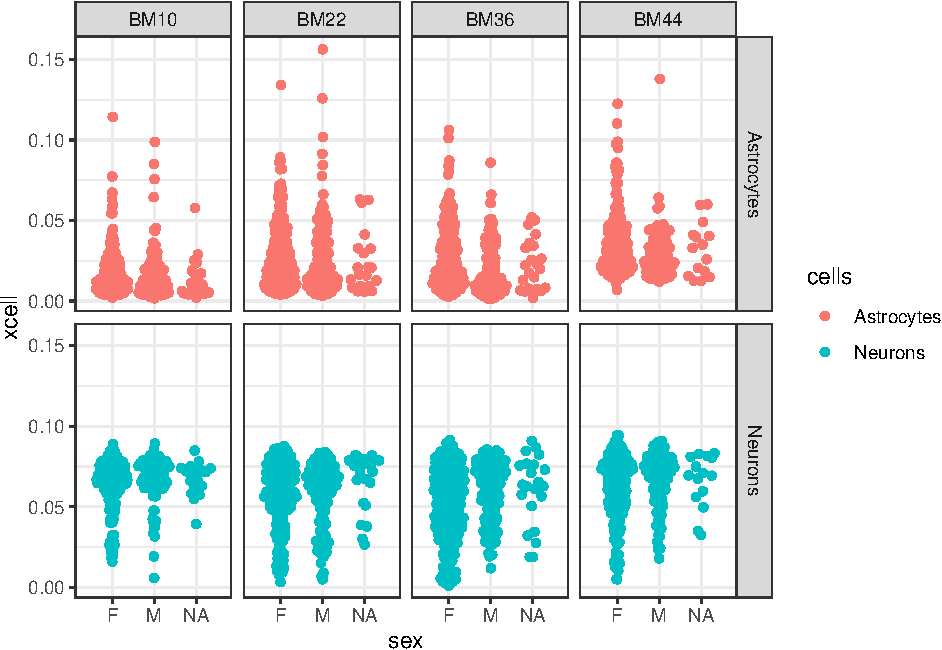
\includegraphics{notebook_files/figure-latex/msbb-rna-dx-plots-3.pdf}

\begin{Shaded}
\begin{Highlighting}[]
\KeywordTok{ggplot}\NormalTok{(msbb_xcell, }\KeywordTok{aes}\NormalTok{(}\DataTypeTok{x =}\NormalTok{ aod, }\DataTypeTok{y =}\NormalTok{ xcell, }\DataTypeTok{colour =}\NormalTok{ ad_reagan)) }\OperatorTok{+}\StringTok{ }
\StringTok{  }\KeywordTok{facet_grid}\NormalTok{(cells }\OperatorTok{~}\StringTok{ }\NormalTok{Tissue) }\OperatorTok{+}
\StringTok{  }\KeywordTok{geom_point}\NormalTok{() }\OperatorTok{+}\StringTok{ }
\StringTok{  }\KeywordTok{geom_smooth}\NormalTok{(}\DataTypeTok{method =}\NormalTok{ lm) }\OperatorTok{+}\StringTok{ }
\StringTok{  }\KeywordTok{theme_bw}\NormalTok{()}
\end{Highlighting}
\end{Shaded}

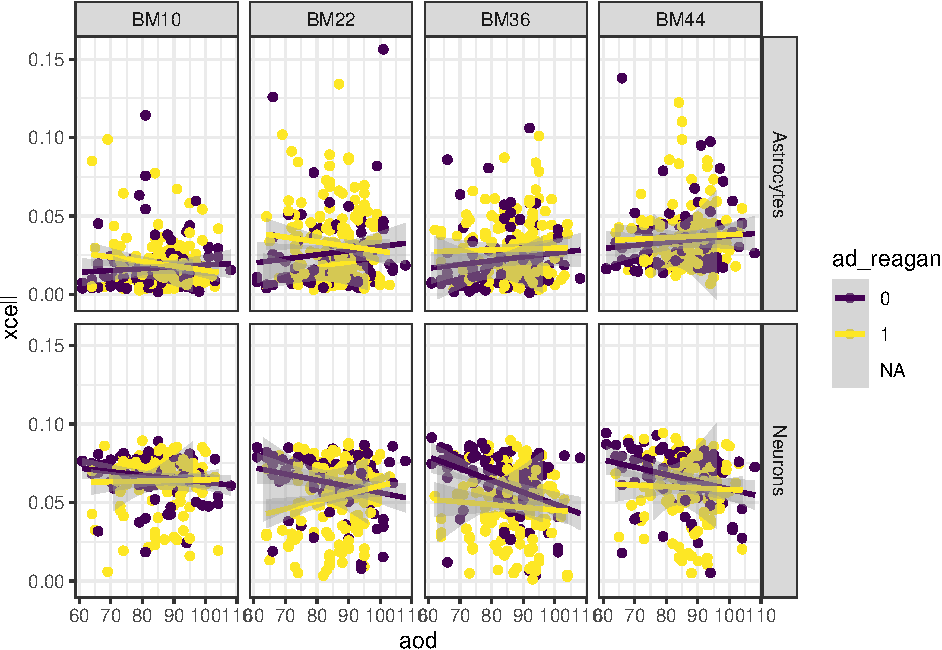
\includegraphics{notebook_files/figure-latex/msbb-rna-dx-plots-4.pdf}

\begin{Shaded}
\begin{Highlighting}[]
\KeywordTok{ggplot}\NormalTok{(msbb_xcell, }\KeywordTok{aes}\NormalTok{(}\DataTypeTok{x =}\NormalTok{ mtcn_avg, }\DataTypeTok{y =}\NormalTok{ xcell, }\DataTypeTok{colour =}\NormalTok{ ad_reagan)) }\OperatorTok{+}\StringTok{ }
\StringTok{  }\KeywordTok{facet_grid}\NormalTok{(cells }\OperatorTok{~}\StringTok{ }\NormalTok{Tissue) }\OperatorTok{+}
\StringTok{  }\KeywordTok{geom_point}\NormalTok{() }\OperatorTok{+}\StringTok{ }
\StringTok{  }\KeywordTok{geom_smooth}\NormalTok{(}\DataTypeTok{method =}\NormalTok{ lm) }\OperatorTok{+}\StringTok{ }
\StringTok{  }\KeywordTok{theme_bw}\NormalTok{()}
\end{Highlighting}
\end{Shaded}

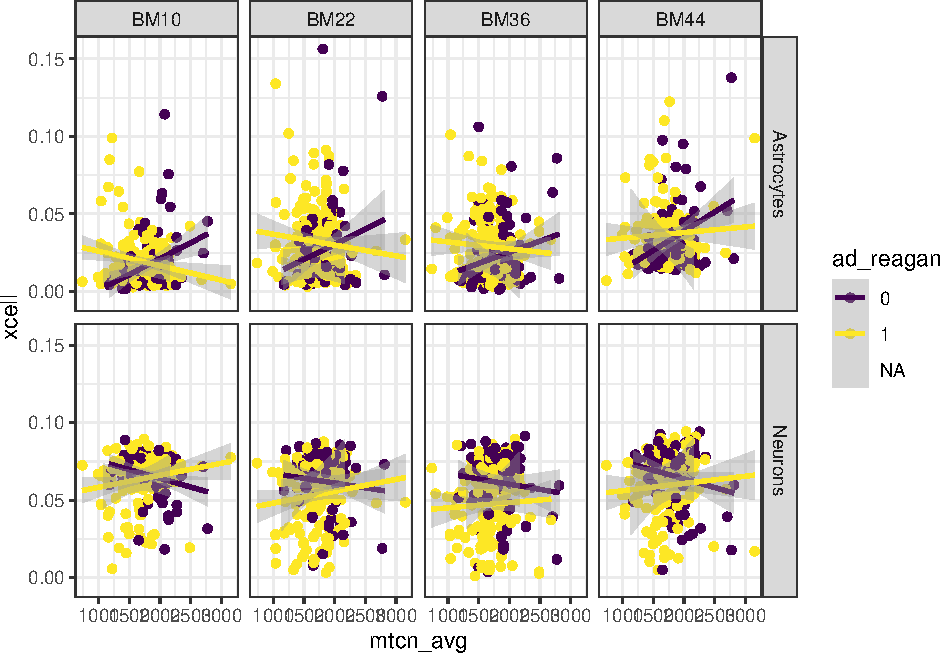
\includegraphics{notebook_files/figure-latex/msbb-rna-dx-plots-5.pdf}

\hypertarget{mayo}{%
\chapter{MAYO}\label{mayo}}

Allen et al \emph{Human whole genome genotype and transcriptome data for Alzheimer's and other neurodegenerative diseases} \href{https://www.nature.com/articles/sdata201689}{Scientific Data 2016}

Mayo Clinic Alzheimer's Disease Genetics Studies (MCADGS). Data is provided for the Mayo RNAseq Study, with whole transcriptome data for 275 Cerebellum (CBE) and 276 Temporal cortex (TCX) samples from 312 North American Caucasian subjects with neuropathological diagnosis of AD, progressive supranuclear palsy (PSP), pathologic aging (PA) or elderly controls (CON) without neurodegenerative diseases. Whole genome sequencing was conducted on 349 participants using DNA isolated from either the Temporal cortex (n = 341) or the Cerebellar Cortex (n = 8).

\begin{itemize}
\tightlist
\item
  All ADs had definite diagnosis according to the NINCDS-ADRDA criteria and had Braak NFT stage of IV or greater.
\item
  Control subjects had Braak NFT stage of III or less, CERAD neuritic and cortical plaque densities of 0 (none) or 1 (sparse) and lacked any of the following pathologic diagnoses: AD, Parkinson's disease (PD), DLB, VaD, PSP, motor neuron disease (MND), CBD, Pick's disease (PiD), Huntington's disease (HD), FTLD, hippocampal sclerosis (HipScl) or dementia lacking distinctive histology (DLDH).
\item
  Subjects with PA also lacked the above diagnoses and had Braak NFT stage of III or less, but had CERAD neuritic and cortical plaque densities of 2 or more. None of the PA subjects had a clinical diagnosis of dementia or mild cognitive impairment.
\end{itemize}

Clinical Code Book: \href{https://adknowledgeportal.synapse.org/Explore/Studies?Study=syn5550404}{Synapse}

\begin{Shaded}
\begin{Highlighting}[]
\CommentTok{## Mayo}
\NormalTok{mayo.raw <-}\StringTok{ }\KeywordTok{read_tsv}\NormalTok{(}\StringTok{'data/AMPAD/mayo/WGS_Metadata.txt'}\NormalTok{) }\OperatorTok
\StringTok{  }\KeywordTok{mutate}\NormalTok{(}\DataTypeTok{WGS_Participant_ID =} \KeywordTok{as.character}\NormalTok{(WGS_Participant_ID), }\DataTypeTok{study =} \StringTok{'MAYO'}\NormalTok{) }
\end{Highlighting}
\end{Shaded}

\begin{verbatim}
Parsed with column specification:
cols(
  WGS_Participant_ID = col_double(),
  Diagnosis = col_character(),
  Sex = col_character(),
  AgeAtDeath = col_character(),
  ApoE = col_double(),
  PMI = col_double(),
  WGS_Source_Tissue_Type = col_character(),
  RNAseq_TCX_SampleID = col_character(),
  RNAseq_TCX_Source = col_character(),
  RNAseq_TCX_Tissue = col_character(),
  RNAseq_TCX_RIN = col_double(),
  RNAseq_TCX_Flowcell = col_character(),
  RNAseq_CER_SampleID = col_character(),
  RNAseq_CER_Source = col_character(),
  RNAseq_CER_Tissue = col_character(),
  RNAseq_CER_RIN = col_double(),
  RNAseq_CER_Flowcell = col_character(),
  files.x = col_character(),
  files.y = col_character()
)
\end{verbatim}

\begin{Shaded}
\begin{Highlighting}[]
\NormalTok{cbe <-}\StringTok{ }\KeywordTok{read_csv}\NormalTok{(}\StringTok{'data/AMPAD_extra/mayo/MayoRNAseq_RNAseq_CER_covariates.csv'}\NormalTok{) }\OperatorTok\StringTok{ }
\StringTok{  }\KeywordTok{mutate}\NormalTok{(}\DataTypeTok{SampleID =} \KeywordTok{str_replace}\NormalTok{(SampleID, }\StringTok{'_CER'}\NormalTok{, }\StringTok{""}\NormalTok{)) }\OperatorTok\StringTok{ }
\StringTok{  }\KeywordTok{select}\NormalTok{(SampleID, Braak, Thal)}
\end{Highlighting}
\end{Shaded}

\begin{verbatim}
Parsed with column specification:
cols(
  SampleID = col_character(),
  Source = col_character(),
  Tissue = col_character(),
  RIN = col_double(),
  Diagnosis = col_character(),
  Sex = col_character(),
  AgeAtDeath = col_character(),
  ApoE = col_double(),
  Flowcell = col_character(),
  PMI = col_double(),
  Braak = col_double(),
  Thal = col_double()
)
\end{verbatim}

\begin{Shaded}
\begin{Highlighting}[]
\NormalTok{tcx  <-}\StringTok{ }\KeywordTok{read_csv}\NormalTok{(}\StringTok{'data/AMPAD_extra/mayo/MayoRNAseq_RNAseq_TCX_covariates.csv'}\NormalTok{)  }\OperatorTok\StringTok{ }
\StringTok{  }\KeywordTok{mutate}\NormalTok{(}\DataTypeTok{SampleID =} \KeywordTok{str_replace}\NormalTok{(SampleID, }\StringTok{'_TCX'}\NormalTok{, }\StringTok{""}\NormalTok{)) }\OperatorTok\StringTok{ }
\StringTok{  }\KeywordTok{rename}\NormalTok{(}\DataTypeTok{Sex =}\NormalTok{ Gender, }\DataTypeTok{Flowcell =}\NormalTok{ FLOWCELL) }\OperatorTok\StringTok{ }
\StringTok{  }\KeywordTok{select}\NormalTok{(SampleID, Braak, Thal) }\OperatorTok\StringTok{ }
\StringTok{  }\KeywordTok{anti_join}\NormalTok{(cbe, }\DataTypeTok{by =} \StringTok{'SampleID'}\NormalTok{) }
\end{Highlighting}
\end{Shaded}

\begin{verbatim}
Parsed with column specification:
cols(
  SampleID = col_character(),
  Source = col_character(),
  Tissue = col_character(),
  RIN = col_double(),
  Diagnosis = col_character(),
  Gender = col_character(),
  AgeAtDeath = col_character(),
  ApoE = col_double(),
  FLOWCELL = col_character(),
  PMI = col_double(),
  Braak = col_double(),
  Thal = col_double()
)
\end{verbatim}

\begin{Shaded}
\begin{Highlighting}[]
\NormalTok{mayo_path <-}\StringTok{ }\KeywordTok{bind_rows}\NormalTok{(cbe, tcx)}

\NormalTok{mosdepth <-}\StringTok{ }\KeywordTok{read_tsv}\NormalTok{(}\StringTok{"data/mosdepth/mosdepth_mtDNAcn_All.txt"}\NormalTok{)}
\end{Highlighting}
\end{Shaded}

\begin{verbatim}
Parsed with column specification:
cols(
  SampleID = col_character(),
  mt_coverage = col_double(),
  autosomal_coverage = col_double(),
  mtcn_avg = col_double()
)
\end{verbatim}

\begin{Shaded}
\begin{Highlighting}[]
\NormalTok{haplogrep <-}\StringTok{ }\KeywordTok{read_tsv}\NormalTok{(}\StringTok{"data/haplogrep/haplogrep_jointAll.txt"}\NormalTok{)}
\end{Highlighting}
\end{Shaded}

\begin{verbatim}
Parsed with column specification:
cols(
  SampleID = col_character(),
  Range = col_character(),
  Haplogroup = col_character(),
  Rank = col_double(),
  Quality = col_double()
)
\end{verbatim}

\begin{Shaded}
\begin{Highlighting}[]
\NormalTok{xcell.raw <-}\StringTok{ }\KeywordTok{read_csv}\NormalTok{(}\StringTok{"data/xcell/ampad_xCell.csv"}\NormalTok{) }
\end{Highlighting}
\end{Shaded}

\begin{verbatim}
Parsed with column specification:
cols(
  SampleID = col_character(),
  Neurons = col_double(),
  Astrocytes = col_double(),
  Neurons.pval = col_double(),
  Astrocytes.pval = col_double(),
  study = col_character(),
  Tissue = col_character(),
  ID = col_character(),
  batch = col_character(),
  RIN = col_double()
)
\end{verbatim}

\begin{Shaded}
\begin{Highlighting}[]
\NormalTok{apoe <-}\StringTok{ }\KeywordTok{read_tsv}\NormalTok{(}\StringTok{"data/AMPAD_extra/mayo/wgs_apoe.tsv"}\NormalTok{) }\OperatorTok\StringTok{ }
\StringTok{  }\KeywordTok{mutate}\NormalTok{(}\DataTypeTok{Indiv =} \KeywordTok{as.character}\NormalTok{(Indiv))}
\end{Highlighting}
\end{Shaded}

\begin{verbatim}
Parsed with column specification:
cols(
  Indiv = col_double(),
  rs429358 = col_character(),
  rs7412 = col_character(),
  apoe = col_double()
)
\end{verbatim}

\hypertarget{demographics}{%
\section{Demographics}\label{demographics}}

\label{tab:mayo-demo-n}Variable type: Numeric

col\_name

min

q1

median

mean

q3

max

sd

pcnt\_na

aod

57

76

83

81.03

89

90

8.37

0

\label{tab:mayo-demo-c}Variable type: Factor

col\_name

level

prop

cnt

aod\_cat

80-89

0.40

141

aod\_cat

70-79

0.25

88

aod\_cat

90+

0.23

79

aod\_cat

60-69

0.11

38

aod\_cat

50-59

0.01

3

race

W

1.00

349

sex

F

0.52

182

sex

M

0.48

167

\hypertarget{plots}{%
\subsection{Plots}\label{plots}}

\begin{Shaded}
\begin{Highlighting}[]
\NormalTok{demo_n }\OperatorTok\StringTok{ }\KeywordTok{show_plot}\NormalTok{()}
\end{Highlighting}
\end{Shaded}

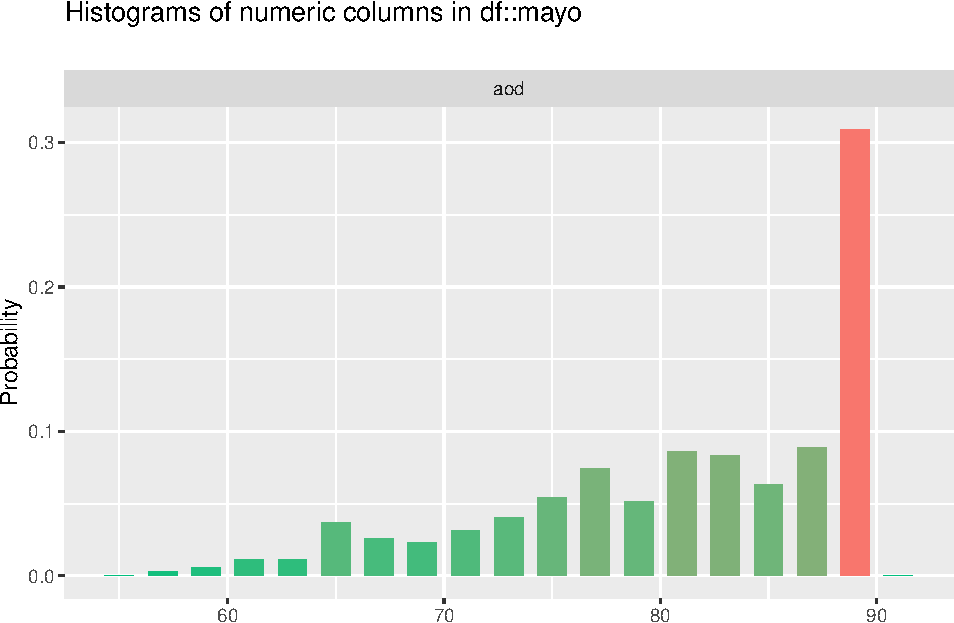
\includegraphics{notebook_files/figure-latex/mayo-plot-demo-1.pdf}

\begin{Shaded}
\begin{Highlighting}[]
\NormalTok{demo_c }\OperatorTok\StringTok{ }\KeywordTok{show_plot}\NormalTok{(}\DataTypeTok{high_cardinality =} \DecValTok{5}\NormalTok{)}
\end{Highlighting}
\end{Shaded}

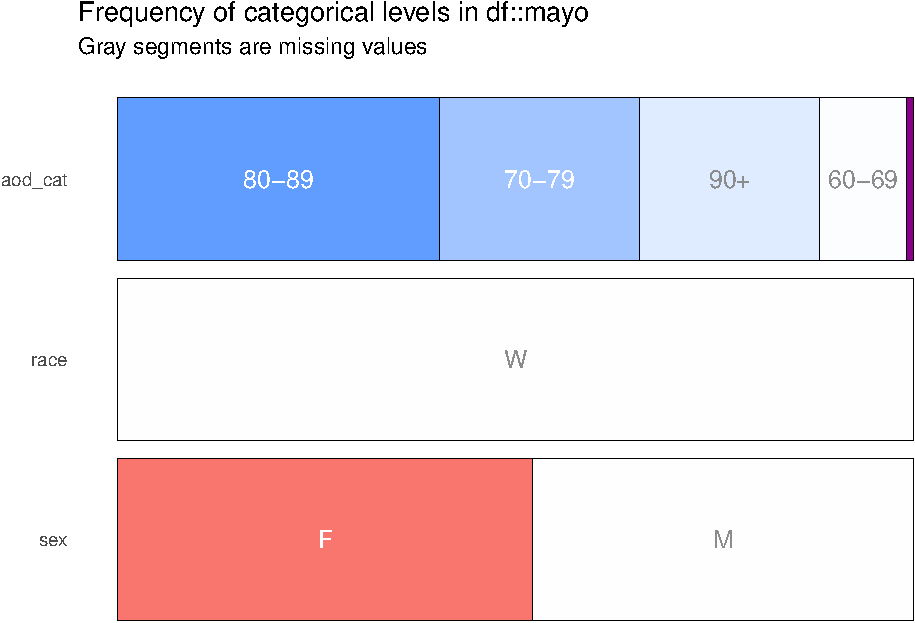
\includegraphics{notebook_files/figure-latex/mayo-plot-demo-2.pdf}

\hypertarget{diagnosis-and-pathology}{%
\section{Diagnosis and Pathology}\label{diagnosis-and-pathology}}

\label{tab:mayo-dx-c}Variable type: Factor

col\_name

level

prop

cnt

braaksc

NA

0.40

141

braaksc

6

0.13

47

braaksc

2

0.11

40

braaksc

3

0.11

40

braaksc

5

0.11

38

braaksc

1

0.05

19

braaksc

0

0.05

18

braaksc

4

0.02

6

dx

Control

0.29

100

dx

AD

0.26

92

dx

PSP

0.24

83

dx

Pathologic Aging

0.21

74

thal

NA

0.55

192

thal

5

0.16

57

thal

0

0.13

46

thal

1

0.08

27

thal

3

0.04

15

thal

2

0.03

9

thal

4

0.01

3

\hypertarget{plots-1}{%
\subsection{Plots}\label{plots-1}}

\begin{Shaded}
\begin{Highlighting}[]
\NormalTok{dx_c }\OperatorTok\StringTok{ }\KeywordTok{show_plot}\NormalTok{(}\DataTypeTok{high_cardinality =} \DecValTok{5}\NormalTok{)}
\end{Highlighting}
\end{Shaded}

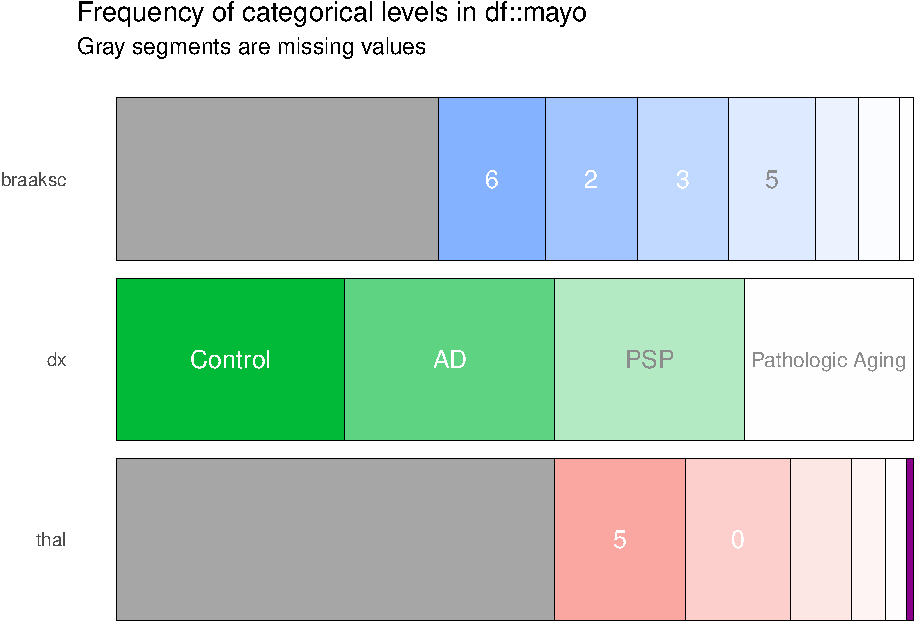
\includegraphics{notebook_files/figure-latex/mayo-plot-dx-1.pdf}

\begin{Shaded}
\begin{Highlighting}[]
\KeywordTok{ggplot}\NormalTok{(}\DataTypeTok{data =}\NormalTok{ mayo) }\OperatorTok{+}
\StringTok{   }\KeywordTok{geom_mosaic}\NormalTok{(}\KeywordTok{aes}\NormalTok{(}\DataTypeTok{x =} \KeywordTok{product}\NormalTok{(dx), }\DataTypeTok{fill=}\NormalTok{thal), }\DataTypeTok{na.rm=}\OtherTok{FALSE}\NormalTok{) }\OperatorTok{+}
\StringTok{  }\KeywordTok{theme_bw}\NormalTok{()}
\end{Highlighting}
\end{Shaded}

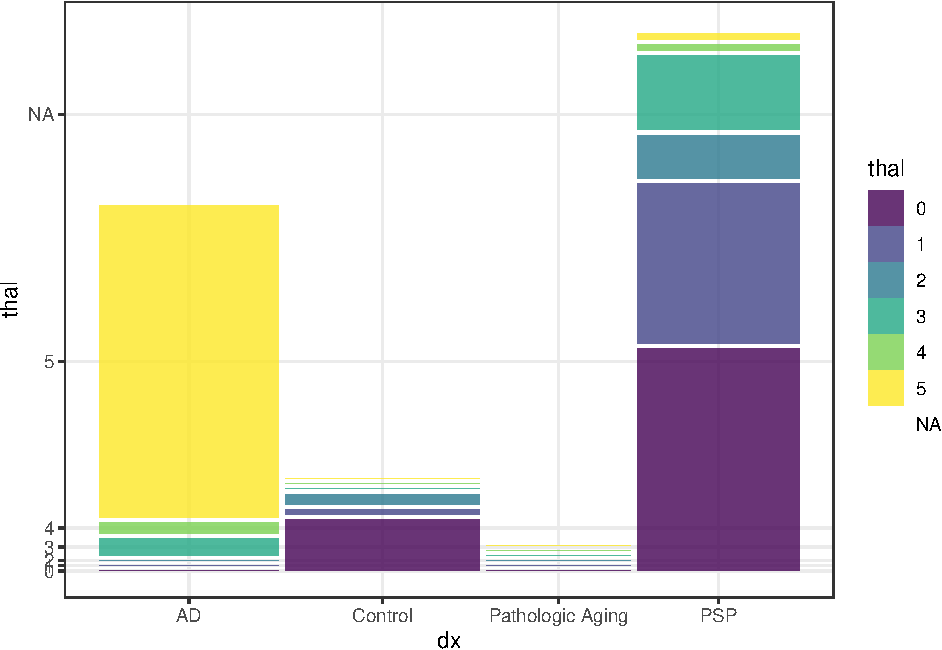
\includegraphics{notebook_files/figure-latex/mayo-plot-dx-2.pdf}

\begin{Shaded}
\begin{Highlighting}[]
   \KeywordTok{labs}\NormalTok{(}\DataTypeTok{x=}\StringTok{"Is it rude recline? "}\NormalTok{, }\DataTypeTok{title=}\StringTok{'f(RudeToRecline)'}\NormalTok{) }
\end{Highlighting}
\end{Shaded}

\begin{verbatim}
$x
[1] "Is it rude recline? "

$title
[1] "f(RudeToRecline)"

attr(,"class")
[1] "labels"
\end{verbatim}

\hypertarget{cross-tabs}{%
\subsection{Cross-tabs}\label{cross-tabs}}

\textbf{Characteristic}

AD

Control

Pathologic Aging

PSP

\textbf{Total}

\textbf{thal}

0

0 (0\%)

10 (2.9\%)

0 (0\%)

36 (10\%)

46 (13\%)

1

0 (0\%)

1 (0.3\%)

0 (0\%)

26 (7.4\%)

27 (7.7\%)

2

0 (0\%)

2 (0.6\%)

0 (0\%)

7 (2.0\%)

9 (2.6\%)

3

3 (0.9\%)

0 (0\%)

0 (0\%)

12 (3.4\%)

15 (4.3\%)

4

2 (0.6\%)

0 (0\%)

0 (0\%)

1 (0.3\%)

3 (0.9\%)

5

56 (16\%)

0 (0\%)

0 (0\%)

1 (0.3\%)

57 (16\%)

Unknown

31 (8.9\%)

87 (25\%)

74 (21\%)

0 (0\%)

192 (55\%)

\textbf{Total}

92 (26\%)

100 (29\%)

74 (21\%)

83 (24\%)

349 (100\%)

\textbf{Characteristic}

AD

Control

Pathologic Aging

PSP

\textbf{Total}

\textbf{braaksc}

0

0 (0\%)

2 (0.6\%)

0 (0\%)

16 (4.6\%)

18 (5.2\%)

1

0 (0\%)

4 (1.1\%)

0 (0\%)

15 (4.3\%)

19 (5.4\%)

2

0 (0\%)

16 (4.6\%)

0 (0\%)

24 (6.9\%)

40 (11\%)

3

0 (0\%)

12 (3.4\%)

0 (0\%)

28 (8.0\%)

40 (11\%)

4

6 (1.7\%)

0 (0\%)

0 (0\%)

0 (0\%)

6 (1.7\%)

5

38 (11\%)

0 (0\%)

0 (0\%)

0 (0\%)

38 (11\%)

6

47 (13\%)

0 (0\%)

0 (0\%)

0 (0\%)

47 (13\%)

Unknown

1 (0.3\%)

66 (19\%)

74 (21\%)

0 (0\%)

141 (40\%)

\textbf{Total}

92 (26\%)

100 (29\%)

74 (21\%)

83 (24\%)

349 (100\%)

\textbf{Characteristic}

0

1

2

3

4

5

Unknown

\textbf{Total}

\textbf{braaksc}

0

10 (2.9\%)

4 (1.1\%)

1 (0.3\%)

2 (0.6\%)

1 (0.3\%)

0 (0\%)

0 (0\%)

18 (5.2\%)

1

8 (2.3\%)

6 (1.7\%)

2 (0.6\%)

1 (0.3\%)

0 (0\%)

0 (0\%)

2 (0.6\%)

19 (5.4\%)

2

10 (2.9\%)

8 (2.3\%)

4 (1.1\%)

6 (1.7\%)

0 (0\%)

1 (0.3\%)

11 (3.2\%)

40 (11\%)

3

18 (5.2\%)

9 (2.6\%)

2 (0.6\%)

3 (0.9\%)

0 (0\%)

0 (0\%)

8 (2.3\%)

40 (11\%)

4

0 (0\%)

0 (0\%)

0 (0\%)

0 (0\%)

0 (0\%)

3 (0.9\%)

3 (0.9\%)

6 (1.7\%)

5

0 (0\%)

0 (0\%)

0 (0\%)

2 (0.6\%)

1 (0.3\%)

21 (6.0\%)

14 (4.0\%)

38 (11\%)

6

0 (0\%)

0 (0\%)

0 (0\%)

1 (0.3\%)

1 (0.3\%)

32 (9.2\%)

13 (3.7\%)

47 (13\%)

Unknown

0 (0\%)

0 (0\%)

0 (0\%)

0 (0\%)

0 (0\%)

0 (0\%)

141 (40\%)

141 (40\%)

\textbf{Total}

46 (13\%)

27 (7.7\%)

9 (2.6\%)

15 (4.3\%)

3 (0.9\%)

57 (16\%)

192 (55\%)

349 (100\%)

\hypertarget{genetics-mitochondria}{%
\section{Genetics \& Mitochondria}\label{genetics-mitochondria}}

\label{tab:mayo-gen-n}Variable type: Numeric

col\_name

min

q1

median

mean

q3

max

sd

pcnt\_na

Quality

0.50

0.91

0.93

0.92

0.96

1.00

0.06

0

mtcn\_avg

437.31

1233.11

1525.57

1549.70

1890.77

2951.37

478.97

0

\label{tab:mayo-gen-c}Variable type: Factor

col\_name

level

prop

cnt

apoe4

e4-

0.72

250

apoe4

e4+

0.28

99

Haplogroup

Other

0.90

315

Haplogroup

H5a1

0.03

10

Haplogroup

H1a

0.02

8

Haplogroup

H1b1+16362

0.02

8

Haplogroup

T2b

0.02

8

macro

H

0.50

174

macro

U

0.13

46

macro

T

0.11

39

macro

J

0.09

31

macro

K

0.07

25

macro

I

0.02

8

macro

V

0.02

8

macro

W

0.01

5

macro

HV

0.01

4

macro

X

0.01

4

macro

M

0.01

2

macro

N

0.01

2

macro

A

0.00

1

SourceTissue

Temporal Cortex

0.98

341

SourceTissue

Cerebellar Cortex

0.02

8

\hypertarget{plots-2}{%
\subsection{Plots}\label{plots-2}}

\begin{Shaded}
\begin{Highlighting}[]
\NormalTok{gen_n }\OperatorTok\StringTok{ }\KeywordTok{show_plot}\NormalTok{()}
\end{Highlighting}
\end{Shaded}

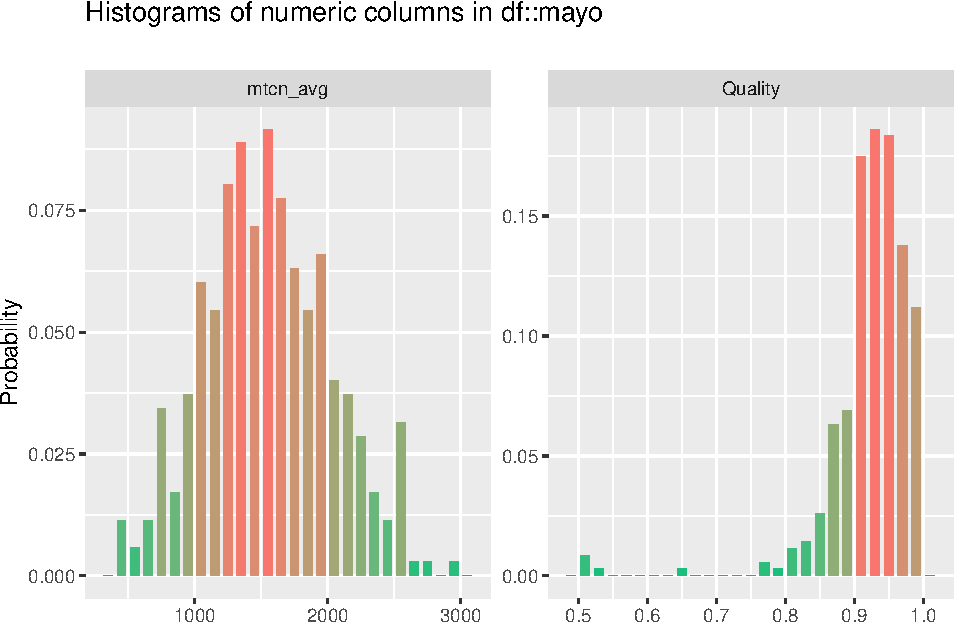
\includegraphics{notebook_files/figure-latex/mayo-plot-gen-1.pdf}

\begin{Shaded}
\begin{Highlighting}[]
\NormalTok{gen_c }\OperatorTok\StringTok{ }\KeywordTok{show_plot}\NormalTok{(}\DataTypeTok{high_cardinality =} \DecValTok{5}\NormalTok{)}
\end{Highlighting}
\end{Shaded}

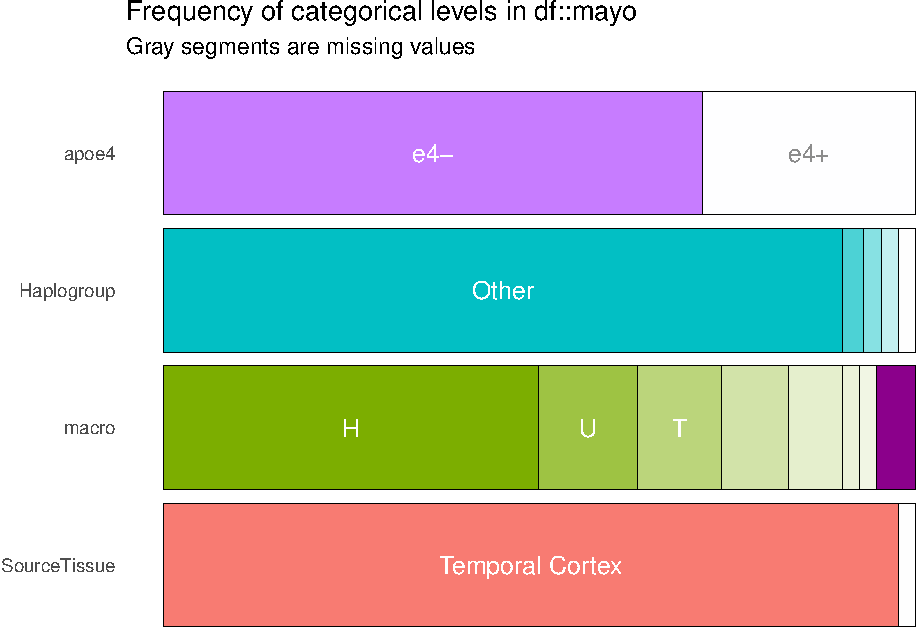
\includegraphics{notebook_files/figure-latex/mayo-plot-gen-2.pdf}

\hypertarget{diagnosis-and-mtdnacn}{%
\subsection{diagnosis and mtDNAcn}\label{diagnosis-and-mtdnacn}}

\begin{Shaded}
\begin{Highlighting}[]
\NormalTok{ mayo }\OperatorTok
\StringTok{    }\KeywordTok{filter}\NormalTok{(}\OperatorTok{!}\KeywordTok{is.na}\NormalTok{(mtcn_avg)) }\OperatorTok
\StringTok{    }\KeywordTok{ggplot}\NormalTok{(., }\KeywordTok{aes}\NormalTok{(}\DataTypeTok{x =}\NormalTok{ SourceTissue, }\DataTypeTok{y =}\NormalTok{ mtcn_avg, }\DataTypeTok{colour =}\NormalTok{ dx)) }\OperatorTok{+}\StringTok{ }
\StringTok{      }\NormalTok{ggbeeswarm}\OperatorTok{::}\KeywordTok{geom_quasirandom}\NormalTok{(}\DataTypeTok{dodge.width=}\DecValTok{1}\NormalTok{) }\OperatorTok{+}\StringTok{ }
\StringTok{      }\KeywordTok{theme_bw}\NormalTok{()}
\end{Highlighting}
\end{Shaded}

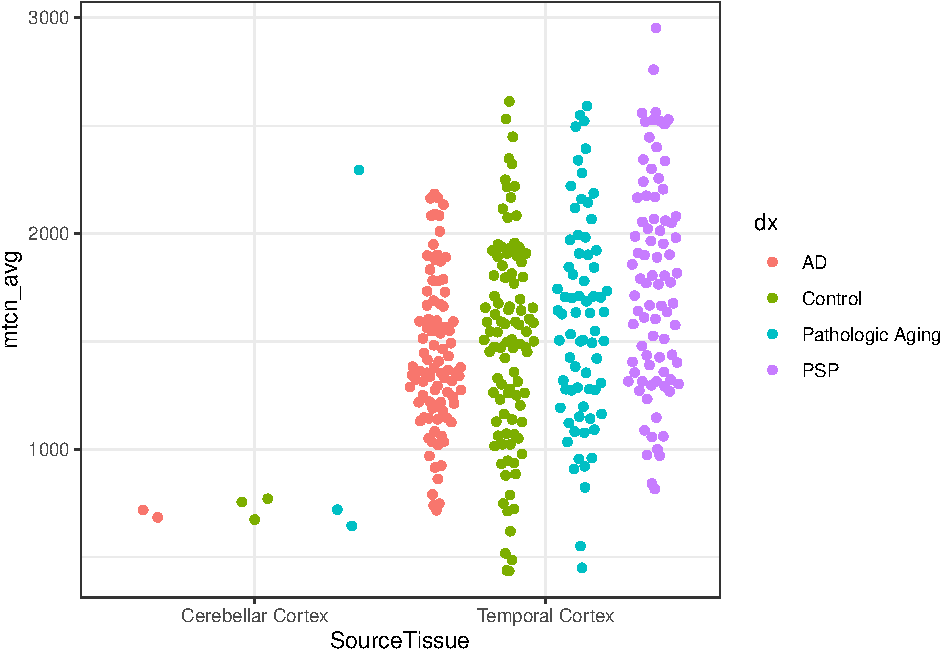
\includegraphics{notebook_files/figure-latex/mayo-dx-mtdnacn-1.pdf}

\hypertarget{rnaseq}{%
\section{RNAseq}\label{rnaseq}}

\label{tab:mayo-rna-numeric}Variable type: Numeric

col\_name

min

q1

median

mean

q3

max

sd

pcnt\_na

Neurons\_CER

0.0

0.05

0.06

0.05

0.06

0.08

0.01

25.79

Neurons\_TCX

0.0

0.04

0.06

0.06

0.07

0.10

0.02

24.64

Astrocytes\_CER

0.0

0.00

0.00

0.01

0.01

0.03

0.00

25.79

Astrocytes\_TCX

0.0

0.02

0.03

0.04

0.04

0.15

0.02

24.64

RIN\_CER

5.5

7.50

8.25

8.13

8.80

10.00

0.95

26.65

RIN\_TCX

5.3

7.90

8.30

8.17

8.70

10.00

0.89

25.21

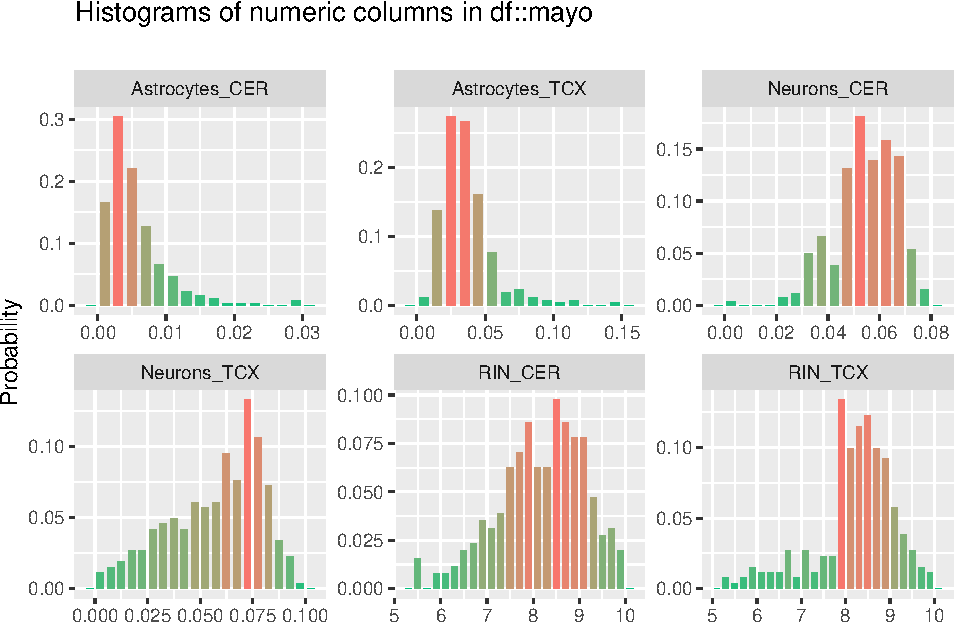
\includegraphics{notebook_files/figure-latex/mayo-rna-plot-1.pdf}

\begin{Shaded}
\begin{Highlighting}[]
\NormalTok{mayo_xcell <-}\StringTok{ }\KeywordTok{select}\NormalTok{(mayo, Neurons, Astrocytes, }
\NormalTok{                       aod, aod_cat, dx, mtcn_avg, sex ) }\OperatorTok\StringTok{ }
\StringTok{  }\KeywordTok{filter}\NormalTok{(}\OperatorTok{!}\KeywordTok{is.na}\NormalTok{(Neurons)) }\OperatorTok\StringTok{ }
\StringTok{  }\KeywordTok{pivot_longer}\NormalTok{(}\KeywordTok{c}\NormalTok{(Neurons, Astrocytes), }\DataTypeTok{names_to =} \StringTok{"cells"}\NormalTok{, }\DataTypeTok{values_to =} \StringTok{"xcell"}\NormalTok{)}

\KeywordTok{ggplot}\NormalTok{(mayo_xcell, }\KeywordTok{aes}\NormalTok{(}\DataTypeTok{x =}\NormalTok{ dx, }\DataTypeTok{y =}\NormalTok{ xcell, }\DataTypeTok{colour =}\NormalTok{ dx)) }\OperatorTok{+}\StringTok{ }
\StringTok{  }\NormalTok{ggbeeswarm}\OperatorTok{::}\KeywordTok{geom_quasirandom}\NormalTok{(}\DataTypeTok{dodge.width=}\DecValTok{1}\NormalTok{) }\OperatorTok{+}\StringTok{ }
\StringTok{  }\KeywordTok{facet_grid}\NormalTok{(cells }\OperatorTok{~}\StringTok{ }\NormalTok{.) }\OperatorTok{+}\StringTok{ }
\StringTok{  }\KeywordTok{theme_bw}\NormalTok{()}
\end{Highlighting}
\end{Shaded}

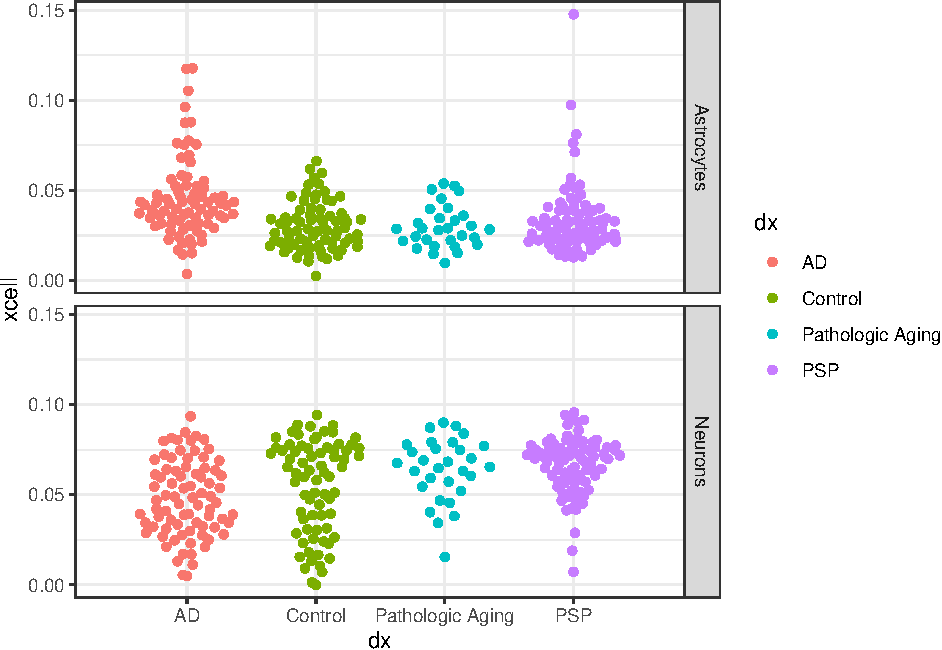
\includegraphics{notebook_files/figure-latex/mayo-rna-dx-plots-1.pdf}

\begin{Shaded}
\begin{Highlighting}[]
\KeywordTok{ggplot}\NormalTok{(mayo_xcell, }\KeywordTok{aes}\NormalTok{(}\DataTypeTok{x =}\NormalTok{ sex, }\DataTypeTok{y =}\NormalTok{ xcell, }\DataTypeTok{colour =}\NormalTok{ cells)) }\OperatorTok{+}\StringTok{ }
\StringTok{  }\NormalTok{ggbeeswarm}\OperatorTok{::}\KeywordTok{geom_quasirandom}\NormalTok{(}\DataTypeTok{dodge.width=}\DecValTok{1}\NormalTok{) }\OperatorTok{+}\StringTok{ }
\StringTok{  }\KeywordTok{facet_grid}\NormalTok{(cells }\OperatorTok{~}\StringTok{ }\NormalTok{.) }\OperatorTok{+}\StringTok{ }
\StringTok{  }\KeywordTok{theme_bw}\NormalTok{()}
\end{Highlighting}
\end{Shaded}

\includegraphics{notebook_files/figure-latex/mayo-rna-dx-plots-2.pdf}

\begin{Shaded}
\begin{Highlighting}[]
\KeywordTok{ggplot}\NormalTok{(mayo_xcell, }\KeywordTok{aes}\NormalTok{(}\DataTypeTok{x =}\NormalTok{ aod, }\DataTypeTok{y =}\NormalTok{ xcell, }\DataTypeTok{colour =}\NormalTok{ dx)) }\OperatorTok{+}\StringTok{ }
\StringTok{  }\KeywordTok{facet_grid}\NormalTok{(cells }\OperatorTok{~}\StringTok{ }\NormalTok{.) }\OperatorTok{+}
\StringTok{  }\KeywordTok{geom_point}\NormalTok{() }\OperatorTok{+}\StringTok{ }
\StringTok{  }\KeywordTok{geom_smooth}\NormalTok{(}\DataTypeTok{method =}\NormalTok{ lm) }\OperatorTok{+}\StringTok{ }
\StringTok{  }\KeywordTok{theme_bw}\NormalTok{()}
\end{Highlighting}
\end{Shaded}

\includegraphics{notebook_files/figure-latex/mayo-rna-dx-plots-3.pdf}

\begin{Shaded}
\begin{Highlighting}[]
\KeywordTok{ggplot}\NormalTok{(mayo_xcell, }\KeywordTok{aes}\NormalTok{(}\DataTypeTok{x =}\NormalTok{ aod_cat, }\DataTypeTok{y =}\NormalTok{ xcell, }\DataTypeTok{colour =}\NormalTok{ dx)) }\OperatorTok{+}\StringTok{ }
\StringTok{  }\KeywordTok{facet_grid}\NormalTok{(cells }\OperatorTok{~}\StringTok{ }\NormalTok{dx) }\OperatorTok{+}
\StringTok{  }\NormalTok{ggbeeswarm}\OperatorTok{::}\KeywordTok{geom_quasirandom}\NormalTok{(}\DataTypeTok{dodge.width=}\DecValTok{1}\NormalTok{) }\OperatorTok{+}\StringTok{ }
\StringTok{  }\KeywordTok{theme_bw}\NormalTok{()}
\end{Highlighting}
\end{Shaded}

\includegraphics{notebook_files/figure-latex/mayo-rna-dx-plots-4.pdf}

\begin{Shaded}
\begin{Highlighting}[]
\KeywordTok{ggplot}\NormalTok{(mayo_xcell, }\KeywordTok{aes}\NormalTok{(}\DataTypeTok{x =}\NormalTok{ mtcn_avg, }\DataTypeTok{y =}\NormalTok{ xcell, }\DataTypeTok{colour =}\NormalTok{ dx)) }\OperatorTok{+}\StringTok{ }
\StringTok{  }\KeywordTok{facet_grid}\NormalTok{(cells }\OperatorTok{~}\StringTok{ }\NormalTok{dx) }\OperatorTok{+}
\StringTok{  }\KeywordTok{geom_point}\NormalTok{() }\OperatorTok{+}\StringTok{ }
\StringTok{  }\KeywordTok{geom_smooth}\NormalTok{(}\DataTypeTok{method =}\NormalTok{ lm) }\OperatorTok{+}\StringTok{ }
\StringTok{  }\KeywordTok{theme_bw}\NormalTok{()}
\end{Highlighting}
\end{Shaded}

\includegraphics{notebook_files/figure-latex/mayo-rna-dx-plots-5.pdf}

\hypertarget{analysis}{%
\chapter{Analysis}\label{analysis}}

\begin{Shaded}
\begin{Highlighting}[]
\CommentTok{# library(MASS)}
\CommentTok{# library(brant)}
\KeywordTok{library}\NormalTok{(VGAM)}
\KeywordTok{library}\NormalTok{(tidyverse)}
\KeywordTok{library}\NormalTok{(broom)}
\KeywordTok{library}\NormalTok{(glue)}
\KeywordTok{library}\NormalTok{(gtsummary)}
\KeywordTok{library}\NormalTok{(gt)}
\NormalTok{knitr}\OperatorTok{::}\NormalTok{opts_knit}\OperatorTok{$}\KeywordTok{set}\NormalTok{(}\DataTypeTok{root.dir =} \StringTok{'/sc/arion/projects/LOAD/shea/Projects/mtDNAcn'}\NormalTok{)}
\KeywordTok{set_gtsummary_theme}\NormalTok{(}\KeywordTok{theme_gtsummary_compact}\NormalTok{())}
\CommentTok{# setwd('/sc/arion/projects/LOAD/shea/Projects/mtDNAcn')}

\CommentTok{## Functions }
\CommentTok{### Tidy VGAM output }
\NormalTok{tidy.vglm <-}\StringTok{ }\ControlFlowTok{function}\NormalTok{(x, }\DataTypeTok{exponentiate =} \OtherTok{FALSE}\NormalTok{, }\DataTypeTok{conf.int=}\OtherTok{FALSE}\NormalTok{, }\DataTypeTok{conf.level=}\FloatTok{0.95}\NormalTok{) \{}
\NormalTok{  co <-}\StringTok{ }\KeywordTok{as.data.frame}\NormalTok{(}\KeywordTok{coef}\NormalTok{(}\KeywordTok{summary}\NormalTok{(x)))}
  \KeywordTok{names}\NormalTok{(co) <-}\StringTok{ }\KeywordTok{c}\NormalTok{(}\StringTok{"estimate"}\NormalTok{,}\StringTok{"std.error"}\NormalTok{,}\StringTok{"statistic"}\NormalTok{,}\StringTok{"p.value"}\NormalTok{)}
  \ControlFlowTok{if}\NormalTok{ (conf.int) \{}
\NormalTok{    qq <-}\StringTok{ }\KeywordTok{qnorm}\NormalTok{((}\DecValTok{1}\OperatorTok{+}\NormalTok{conf.level)}\OperatorTok{/}\DecValTok{2}\NormalTok{)}
\NormalTok{    co <-}\StringTok{ }\KeywordTok{transform}\NormalTok{(co,}
                    \DataTypeTok{conf.low=}\NormalTok{estimate}\OperatorTok{-}\NormalTok{qq}\OperatorTok{*}\NormalTok{std.error,}
                    \DataTypeTok{conf.high=}\NormalTok{estimate}\OperatorTok{+}\NormalTok{qq}\OperatorTok{*}\NormalTok{std.error)}
\NormalTok{  \} }
  \ControlFlowTok{if}\NormalTok{ (exponentiate }\OperatorTok{==}\StringTok{ }\OtherTok{TRUE}\NormalTok{) \{}
\NormalTok{    qq <-}\StringTok{ }\KeywordTok{qnorm}\NormalTok{((}\DecValTok{1}\OperatorTok{+}\NormalTok{conf.level)}\OperatorTok{/}\DecValTok{2}\NormalTok{)}
\NormalTok{    co <-}\StringTok{ }\KeywordTok{transform}\NormalTok{(co,}
                    \DataTypeTok{conf.low=}\NormalTok{estimate}\OperatorTok{-}\NormalTok{qq}\OperatorTok{*}\NormalTok{std.error,}
                    \DataTypeTok{conf.high=}\NormalTok{estimate}\OperatorTok{+}\NormalTok{qq}\OperatorTok{*}\NormalTok{std.error)}
\NormalTok{    co <-}\StringTok{ }\KeywordTok{transform}\NormalTok{(co, }
                    \DataTypeTok{OR =} \KeywordTok{exp}\NormalTok{(estimate), }
                    \DataTypeTok{lci =} \KeywordTok{exp}\NormalTok{(conf.low),}
                    \DataTypeTok{uci =} \KeywordTok{exp}\NormalTok{(conf.high))}
    
\NormalTok{  \}}
\NormalTok{  co <-}\StringTok{ }\KeywordTok{data.frame}\NormalTok{(}\DataTypeTok{term=}\KeywordTok{rownames}\NormalTok{(co),co)}
  \KeywordTok{rownames}\NormalTok{(co) <-}\StringTok{ }\OtherTok{NULL}
\NormalTok{  co <-}\StringTok{ }\KeywordTok{as_tibble}\NormalTok{(co)}
  \KeywordTok{return}\NormalTok{(co)}
\NormalTok{\}}
\end{Highlighting}
\end{Shaded}

\begin{Shaded}
\begin{Highlighting}[]
\NormalTok{rosmap.raw <-}\StringTok{ }\KeywordTok{read_rds}\NormalTok{(}\StringTok{'output/rosmap.rds'}\NormalTok{)}
\NormalTok{msbb.raw <-}\StringTok{ }\KeywordTok{read_rds}\NormalTok{(}\StringTok{'output/msbb.rds'}\NormalTok{)}
\NormalTok{mayo.raw <-}\StringTok{ }\KeywordTok{read_rds}\NormalTok{(}\StringTok{'output/mayo.rds'}\NormalTok{)}
\end{Highlighting}
\end{Shaded}

\hypertarget{statistical-analysis-plan}{%
\section{Statistical Analysis Plan}\label{statistical-analysis-plan}}

\textbf{PLANNED ANALYSIS BY AIMS:} Using whole-genome sequencing and neuropathology from AMP-AD (MSBB, ROSMAP, Mayo) we investigate the assocation of mitochondrial haplogroups and mtDNAcn with neurpathologicaly defined AD and neuropathology.

\textbf{Aim 1:} Investigate the association of mt-hgs with AD neuropathologic change

\emph{Hypothesis 1a:} mt-hgs will be differentially associated with neuropathologicaly confirmed AD.

\emph{Hypothesis 1b:} mt-hgs will be differentially associated with neuropatholgy markers of AD.

\emph{Rational:} mt-hgs have been assocaited with clinically diagnosed AD, however, due to the heterogenity in the underlying neuropathology not all cases or controls may had Alzheimer's disease due to AD neuropathologic change which would weaken the statistical power to determine an association with AD. Secondly, using endophenotypes of AD such as neuropathology may further increase statistical power.

\emph{Primary Proposed Analysis:} AMP-AD cohorts will be limited to non-hispanic whites and European- haplogroups only. For neuropathologicaly confirmed AD, modified regan diagnosis will be used as the outcome for ROSMAP and MSBB, for Mayo Controls+Pathologic Aging and AD diagnosis will be used as outcomes. Logistic regression adjusting for age at death, sex and APOE will be used to evaluate the associations of the mt-hgs with neuropathologicaly confirmed AD seperatly in each cohort. Fixed-effects meta-analysis will be used to measure the combined effect of the haplogroups in AMP-AD. Linear regression will be used to investigate the association with AD neurpathology.

\emph{Anticipated Problems and Alternative Approaches:}

\begin{itemize}
\tightlist
\item
  Sample size: Small cell sizes, in particular for MSBB and Mayo for the mtHgs (i.e.~I, W, X), may result in low statistical power, can alterntivly conduct a joint analysis. Can lump smaller cells into single category (e.g.~IWX)
\item
  Differences in study designs (population based - ROSMAP; case-control - MSBB, Mayo) and neurpathology definitions (ROSMAP + MSBB vs Mayo) may result in between study heterogenity. Additionlay Mayo AOD is censord. This will also limit usability of joint analysis
\item
  Can possibly include ADNI using a A/T/N based diagnosis.
\end{itemize}

\emph{Secondary, exploratory analysis:} Using ROSAMP, we can 1) examine the association of mt-hgs with additional neuropathological measures such as infarcts, TDP-43 and; 2) evaluate differential associations between clinically defined AD and neuropathologicaly confirmed AD.

\hypertarget{data-wrangling}{%
\section{Data Wrangling}\label{data-wrangling}}

\hypertarget{rosmap}{%
\subsection{ROSMAP}\label{rosmap}}

\begin{itemize}
\tightlist
\item
  Neuropatholgical Diagnosis, i.e.~individuals who have died
\item
  Caucasians only
\item
  Haplogroups

  \begin{itemize}
  \tightlist
  \item
    European haplogroups (H, V, J, T, U, K, I, W, X)
  \item
    Quality \textgreater{} 0.8
  \item
    lump Hgs IWX
  \end{itemize}
\end{itemize}

\begin{Shaded}
\begin{Highlighting}[]
\NormalTok{rosmap_df <-}\StringTok{ }\NormalTok{rosmap.raw }\OperatorTok\StringTok{ }
\StringTok{  }\KeywordTok{mutate}\NormalTok{(}\DataTypeTok{id =} \KeywordTok{paste0}\NormalTok{(study, projid)) }\OperatorTok
\StringTok{  }\KeywordTok{select}\NormalTok{(id, study, apoe_genotype, apoe4, age_death, aod_cat, msex, race7, spanish, pmi, }
\NormalTok{         ad_reagan, niareagansc, cogdx,}
\NormalTok{         Haplogroup, macro, Quality, }
\NormalTok{         ceradsc, braaksc, gpath, amyloid, plaq_d, plaq_n, tangles, nft, }
\NormalTok{         dlbdx, ci_num2_gct, ci_num2_mct, cvda_4gp2, caa_4gp, arteriol_scler, hspath_typ, tdp_st4) }\OperatorTok
\StringTok{  }\KeywordTok{distinct}\NormalTok{(id, }\DataTypeTok{.keep_all =} \OtherTok{TRUE}\NormalTok{) }\OperatorTok\StringTok{ }
\StringTok{  }\KeywordTok{filter}\NormalTok{(}\OperatorTok{!}\KeywordTok{is.na}\NormalTok{(age_death)) }\OperatorTok\StringTok{ }
\StringTok{  }\KeywordTok{filter}\NormalTok{(macro }\OperatorTok\StringTok{ }\KeywordTok{c}\NormalTok{(}\StringTok{'H'}\NormalTok{, }\StringTok{'V'}\NormalTok{, }\StringTok{'J'}\NormalTok{, }\StringTok{'T'}\NormalTok{, }\StringTok{'U'}\NormalTok{, }\StringTok{'K'}\NormalTok{, }\StringTok{'I'}\NormalTok{, }\StringTok{'W'}\NormalTok{, }\StringTok{'X'}\NormalTok{)) }\OperatorTok
\StringTok{  }\KeywordTok{filter}\NormalTok{(Quality }\OperatorTok{>}\StringTok{ }\FloatTok{0.8}\NormalTok{) }\OperatorTok
\StringTok{  }\KeywordTok{mutate}\NormalTok{(}\DataTypeTok{aod_cat =} \KeywordTok{fct_expand}\NormalTok{(aod_cat, }\StringTok{"50-59"}\NormalTok{), }
         \DataTypeTok{ad_reagan =} \KeywordTok{factor}\NormalTok{(ad_reagan), }
         \DataTypeTok{ad_reagan =} \KeywordTok{fct_relevel}\NormalTok{(ad_reagan, }\StringTok{"0"}\NormalTok{, }\StringTok{"1"}\NormalTok{), }
         \DataTypeTok{macro_lmp =} \KeywordTok{fct_recode}\NormalTok{(macro, }\StringTok{"H"}\NormalTok{ =}\StringTok{ "H"}\NormalTok{, }\StringTok{"V"}\NormalTok{ =}\StringTok{ "V"}\NormalTok{, }\StringTok{"J"}\NormalTok{ =}\StringTok{ "J"}\NormalTok{, }\StringTok{"T"}\NormalTok{ =}\StringTok{ "T"}\NormalTok{, }\StringTok{"U"}\NormalTok{ =}\StringTok{ "U"}\NormalTok{, }\StringTok{"K"}\NormalTok{ =}\StringTok{ "K"}\NormalTok{,}
                                \StringTok{"IWX"}\NormalTok{ =}\StringTok{ "I"}\NormalTok{, }\StringTok{"IWX"}\NormalTok{ =}\StringTok{ "W"}\NormalTok{, }\StringTok{"IWX"}\NormalTok{ =}\StringTok{ "X"}\NormalTok{),}
         \DataTypeTok{aod_cat2 =} \KeywordTok{factor}\NormalTok{(aod_cat, }\DataTypeTok{ordered =} \OtherTok{FALSE}\NormalTok{), }
         \DataTypeTok{aod_cat =} \KeywordTok{fct_recode}\NormalTok{(aod_cat, }\StringTok{"50-69"}\NormalTok{ =}\StringTok{ "50-59"}\NormalTok{, }\StringTok{"50-69"}\NormalTok{ =}\StringTok{ "60-69"}\NormalTok{)) }\OperatorTok
\StringTok{  }\KeywordTok{rename}\NormalTok{(}\DataTypeTok{dx =}\NormalTok{ ad_reagan, }\DataTypeTok{aod =}\NormalTok{ age_death, }\DataTypeTok{sex =}\NormalTok{ msex)}

\NormalTok{t1 <-}\StringTok{ }\NormalTok{rosmap_df }\OperatorTok\StringTok{ }
\StringTok{  }\KeywordTok{select}\NormalTok{(dx, aod, }\DataTypeTok{aod_cat =}\NormalTok{ aod_cat2, apoe4, sex, macro) }\OperatorTok\StringTok{ }
\StringTok{  }\KeywordTok{mutate}\NormalTok{(}\DataTypeTok{aod_cat =} \KeywordTok{factor}\NormalTok{(aod_cat, }\DataTypeTok{ordered =} \OtherTok{FALSE}\NormalTok{)) }\OperatorTok
\StringTok{  }\KeywordTok{tbl_summary}\NormalTok{(. , }\DataTypeTok{by =}\NormalTok{ dx, }
              \DataTypeTok{statistic =} \KeywordTok{list}\NormalTok{(}\KeywordTok{all_continuous}\NormalTok{() }\OperatorTok{~}\StringTok{ "\{mean\} (\{sd\})"}\NormalTok{, }
                               \KeywordTok{all_categorical}\NormalTok{() }\OperatorTok{~}\StringTok{ "\{n\} (\{p\}%)"}\NormalTok{)}
\NormalTok{              ) }
\end{Highlighting}
\end{Shaded}

\hypertarget{msbb}{%
\subsection{MSBB}\label{msbb}}

\begin{itemize}
\tightlist
\item
  Exclude individules who are not non-hispanic whites
\item
  Haplogroups

  \begin{itemize}
  \tightlist
  \item
    European haplogroups (H, V, J, T, U, K, I, W, X)
  \item
    Quality \textgreater{} 0.8
  \item
    lump Hgs IWX
  \end{itemize}
\item
  Dichotomize CERAD dx
\end{itemize}

\begin{Shaded}
\begin{Highlighting}[]
\NormalTok{msbb_df <-}\StringTok{ }\NormalTok{msbb.raw  }\OperatorTok\StringTok{ }
\StringTok{  }\KeywordTok{select}\NormalTok{(id, study, sex, race, }\DataTypeTok{pmi =}\NormalTok{ PMI, aod, aod_cat, apoe, apoe4,}
\NormalTok{         niareagansc, ad_reagan, cerad, ceradsc, braaksc, }
\NormalTok{         Haplogroup, macro, Quality) }\OperatorTok
\StringTok{  }\KeywordTok{filter}\NormalTok{(}\OperatorTok{!}\KeywordTok{is.na}\NormalTok{(aod)) }\OperatorTok
\StringTok{  }\KeywordTok{filter}\NormalTok{(race }\OperatorTok{==}\StringTok{ 'W'}\NormalTok{) }\OperatorTok
\StringTok{  }\KeywordTok{filter}\NormalTok{(macro }\OperatorTok\StringTok{ }\KeywordTok{c}\NormalTok{(}\StringTok{'H'}\NormalTok{, }\StringTok{'V'}\NormalTok{, }\StringTok{'J'}\NormalTok{, }\StringTok{'T'}\NormalTok{, }\StringTok{'U'}\NormalTok{, }\StringTok{'K'}\NormalTok{, }\StringTok{'I'}\NormalTok{, }\StringTok{'W'}\NormalTok{, }\StringTok{'X'}\NormalTok{)) }\OperatorTok\StringTok{ }
\StringTok{  }\KeywordTok{filter}\NormalTok{(Quality }\OperatorTok{>}\StringTok{ }\FloatTok{0.8}\NormalTok{) }\OperatorTok
\StringTok{  }\KeywordTok{mutate}\NormalTok{(}\DataTypeTok{dx =} \KeywordTok{factor}\NormalTok{(ad_reagan, }\DataTypeTok{ordered =} \OtherTok{FALSE}\NormalTok{),}
         \DataTypeTok{aod_cat =} \KeywordTok{fct_expand}\NormalTok{(aod_cat, }\StringTok{"50-59"}\NormalTok{), }
         \DataTypeTok{cerad_dx =} \KeywordTok{fct_recode}\NormalTok{(cerad, }\StringTok{"0"}\NormalTok{ =}\StringTok{ "Normal"}\NormalTok{, }\StringTok{"0"}\NormalTok{ =}\StringTok{ "Possible"}\NormalTok{, }\StringTok{"1"}\NormalTok{ =}\StringTok{ "Probable"}\NormalTok{, }\StringTok{"1"}\NormalTok{ =}\StringTok{ "Definite"}\NormalTok{), }
         \DataTypeTok{macro_lmp =} \KeywordTok{fct_recode}\NormalTok{(macro, }\StringTok{"H"}\NormalTok{ =}\StringTok{ "H"}\NormalTok{, }\StringTok{"V"}\NormalTok{ =}\StringTok{ "V"}\NormalTok{, }\StringTok{"J"}\NormalTok{ =}\StringTok{ "J"}\NormalTok{, }\StringTok{"T"}\NormalTok{ =}\StringTok{ "T"}\NormalTok{, }\StringTok{"U"}\NormalTok{ =}\StringTok{ "U"}\NormalTok{, }\StringTok{"K"}\NormalTok{ =}\StringTok{ "K"}\NormalTok{,}
                                \StringTok{"IWX"}\NormalTok{ =}\StringTok{ "I"}\NormalTok{, }\StringTok{"IWX"}\NormalTok{ =}\StringTok{ "W"}\NormalTok{, }\StringTok{"IWX"}\NormalTok{ =}\StringTok{ "X"}\NormalTok{),}
         \DataTypeTok{aod_cat2 =} \KeywordTok{factor}\NormalTok{(aod_cat, }\DataTypeTok{ordered =} \OtherTok{FALSE}\NormalTok{), }
         \DataTypeTok{aod_cat =} \KeywordTok{fct_recode}\NormalTok{(aod_cat, }\StringTok{"50-69"}\NormalTok{ =}\StringTok{ "50-59"}\NormalTok{, }\StringTok{"50-69"}\NormalTok{ =}\StringTok{ "60-69"}\NormalTok{) )}

\NormalTok{t2 <-}\StringTok{ }\NormalTok{msbb_df }\OperatorTok\StringTok{ }
\StringTok{  }\KeywordTok{select}\NormalTok{(dx, aod, }\DataTypeTok{aod_cat =}\NormalTok{ aod_cat2, apoe4, sex, macro) }\OperatorTok\StringTok{ }
\StringTok{  }\KeywordTok{mutate}\NormalTok{(}\DataTypeTok{dx =} \KeywordTok{fct_recode}\NormalTok{(dx, }\StringTok{"AD"}\NormalTok{ =}\StringTok{ "1"}\NormalTok{, }\StringTok{"CTRL"}\NormalTok{ =}\StringTok{ "0"}\NormalTok{)) }\OperatorTok
\StringTok{  }\KeywordTok{tbl_summary}\NormalTok{(. , }\DataTypeTok{by =}\NormalTok{ dx,}
              \DataTypeTok{statistic =} \KeywordTok{list}\NormalTok{(}\KeywordTok{all_continuous}\NormalTok{() }\OperatorTok{~}\StringTok{ "\{mean\} (\{sd\})"}\NormalTok{, }
                               \KeywordTok{all_categorical}\NormalTok{() }\OperatorTok{~}\StringTok{ "\{n\} (\{p\}%)"}\NormalTok{)}
\NormalTok{) }
\end{Highlighting}
\end{Shaded}

\hypertarget{mayo}{%
\subsection{Mayo}\label{mayo}}

\begin{itemize}
\tightlist
\item
  Exclude individules who are not non-hispanic whites
\item
  Haplogroups

  \begin{itemize}
  \tightlist
  \item
    European haplogroups (H, V, J, T, U, K, I, W, X)
  \item
    Quality \textgreater{} 0.8
  \item
    lump Hgs IWX
  \end{itemize}
\item
  Diagnosis

  \begin{itemize}
  \tightlist
  \item
    Exclude PSP
  \item
    Collapse controls and pathologic aging
  \end{itemize}
\item
  Age of Death is censored

  \begin{itemize}
  \tightlist
  \item
    Collapse 50-59 / 60-69
  \end{itemize}
\end{itemize}

\begin{Shaded}
\begin{Highlighting}[]
\NormalTok{mayo_df <-}\StringTok{ }\NormalTok{mayo.raw }\OperatorTok\StringTok{ }
\StringTok{  }\KeywordTok{select}\NormalTok{(}\OperatorTok{-}\NormalTok{SourceTissue, }\OperatorTok{-}\NormalTok{mtcn_avg) }\OperatorTok\StringTok{ }
\StringTok{  }\KeywordTok{filter}\NormalTok{(macro }\OperatorTok\StringTok{ }\KeywordTok{c}\NormalTok{(}\StringTok{'H'}\NormalTok{, }\StringTok{'V'}\NormalTok{, }\StringTok{'J'}\NormalTok{, }\StringTok{'T'}\NormalTok{, }\StringTok{'U'}\NormalTok{, }\StringTok{'K'}\NormalTok{, }\StringTok{'I'}\NormalTok{, }\StringTok{'W'}\NormalTok{, }\StringTok{'X'}\NormalTok{)) }\OperatorTok\StringTok{ }
\StringTok{  }\KeywordTok{filter}\NormalTok{(Quality }\OperatorTok{>}\StringTok{ }\FloatTok{0.8}\NormalTok{) }\OperatorTok
\StringTok{  }\KeywordTok{filter}\NormalTok{(dx }\OperatorTok{!=}\StringTok{ "PSP"}\NormalTok{) }\OperatorTok
\StringTok{  }\KeywordTok{mutate}\NormalTok{(}\DataTypeTok{dx =} \KeywordTok{fct_drop}\NormalTok{(dx), }
         \DataTypeTok{dx =} \KeywordTok{fct_recode}\NormalTok{(dx, }\StringTok{"0"}\NormalTok{ =}\StringTok{ "Control"}\NormalTok{, }\StringTok{"0"}\NormalTok{ =}\StringTok{ "Pathologic Aging"}\NormalTok{, }\StringTok{"1"}\NormalTok{ =}\StringTok{ "AD"}\NormalTok{), }
         \DataTypeTok{macro_lmp =} \KeywordTok{fct_recode}\NormalTok{(macro, }\StringTok{"H"}\NormalTok{ =}\StringTok{ "H"}\NormalTok{, }\StringTok{"V"}\NormalTok{ =}\StringTok{ "V"}\NormalTok{, }\StringTok{"J"}\NormalTok{ =}\StringTok{ "J"}\NormalTok{, }\StringTok{"T"}\NormalTok{ =}\StringTok{ "T"}\NormalTok{, }\StringTok{"U"}\NormalTok{ =}\StringTok{ "U"}\NormalTok{, }\StringTok{"K"}\NormalTok{ =}\StringTok{ "K"}\NormalTok{,}
                                \StringTok{"IWX"}\NormalTok{ =}\StringTok{ "I"}\NormalTok{, }\StringTok{"IWX"}\NormalTok{ =}\StringTok{ "W"}\NormalTok{, }\StringTok{"IWX"}\NormalTok{ =}\StringTok{ "X"}\NormalTok{), }
         \DataTypeTok{aod_cat2 =} \KeywordTok{factor}\NormalTok{(aod_cat, }\DataTypeTok{ordered =} \OtherTok{FALSE}\NormalTok{), }
         \DataTypeTok{aod_cat =} \KeywordTok{fct_recode}\NormalTok{(aod_cat, }\StringTok{"50-69"}\NormalTok{ =}\StringTok{ "50-59"}\NormalTok{, }\StringTok{"50-69"}\NormalTok{ =}\StringTok{ "60-69"}\NormalTok{)) }
         
\NormalTok{t3 <-}\StringTok{ }\NormalTok{mayo_df }\OperatorTok\StringTok{ }
\StringTok{  }\KeywordTok{select}\NormalTok{(dx, }\DataTypeTok{aod_cat =}\NormalTok{ aod_cat2, apoe4, sex, macro) }\OperatorTok\StringTok{ }
\StringTok{  }\KeywordTok{mutate}\NormalTok{(}\DataTypeTok{dx =} \KeywordTok{fct_recode}\NormalTok{(dx, }\StringTok{"AD"}\NormalTok{ =}\StringTok{ "1"}\NormalTok{, }\StringTok{"CTRL"}\NormalTok{ =}\StringTok{ "0"}\NormalTok{)) }\OperatorTok
\StringTok{  }\KeywordTok{tbl_summary}\NormalTok{(. , }\DataTypeTok{by =}\NormalTok{ dx,}
              \DataTypeTok{statistic =} \KeywordTok{list}\NormalTok{(}\KeywordTok{all_continuous}\NormalTok{() }\OperatorTok{~}\StringTok{ "\{mean\} (\{sd\})"}\NormalTok{, }
                               \KeywordTok{all_categorical}\NormalTok{() }\OperatorTok{~}\StringTok{ "\{n\} (\{p\}%)"}\NormalTok{)}
\NormalTok{) }
\end{Highlighting}
\end{Shaded}

\hypertarget{joint}{%
\subsection{Joint}\label{joint}}

\begin{Shaded}
\begin{Highlighting}[]
\NormalTok{ampad <-}\StringTok{ }\KeywordTok{bind_rows}\NormalTok{(}
  \KeywordTok{select}\NormalTok{(rosmap_df, id, study, dx, niareagansc, ceradsc, braaksc, aod, aod_cat, apoe4, sex, pmi, macro, macro_lmp),}
  \KeywordTok{select}\NormalTok{(msbb_df, id, study, dx, ceradsc, niareagansc, braaksc, aod, aod_cat, apoe4, sex, pmi, macro, macro_lmp),}
  \KeywordTok{select}\NormalTok{(mayo_df, id, study, dx, thal, braaksc, aod, aod_cat, apoe4, sex, macro, pmi, macro_lmp)}
\NormalTok{) }
\end{Highlighting}
\end{Shaded}

\begin{Shaded}
\begin{Highlighting}[]
\NormalTok{ampad }\OperatorTok\StringTok{ }
\StringTok{  }\KeywordTok{mutate}\NormalTok{(}\DataTypeTok{niareagansc =} \KeywordTok{factor}\NormalTok{(niareagansc, }\DataTypeTok{ordered =} \OtherTok{FALSE}\NormalTok{),}
         \DataTypeTok{ceradsc =} \KeywordTok{factor}\NormalTok{(ceradsc, }\DataTypeTok{ordered =} \OtherTok{FALSE}\NormalTok{),}
         \DataTypeTok{braaksc =} \KeywordTok{factor}\NormalTok{(braaksc, }\DataTypeTok{ordered =} \OtherTok{FALSE}\NormalTok{),}
         \DataTypeTok{thal =} \KeywordTok{factor}\NormalTok{(thal, }\DataTypeTok{ordered =} \OtherTok{FALSE}\NormalTok{), }
         \DataTypeTok{aod_cat =} \KeywordTok{factor}\NormalTok{(aod_cat, }\DataTypeTok{ordered =} \OtherTok{FALSE}\NormalTok{)) }\OperatorTok
\StringTok{  }\KeywordTok{select}\NormalTok{(}\OperatorTok{-}\NormalTok{id, }\OperatorTok{-}\NormalTok{macro_lmp) }\OperatorTok
\StringTok{  }\KeywordTok{tbl_summary}\NormalTok{(., }\DataTypeTok{by =}\NormalTok{ study,}
              \DataTypeTok{statistic =} \KeywordTok{list}\NormalTok{(}\KeywordTok{all_continuous}\NormalTok{() }\OperatorTok{~}\StringTok{ "\{mean\} (\{sd\})"}\NormalTok{, }
                               \KeywordTok{all_categorical}\NormalTok{() }\OperatorTok{~}\StringTok{ "\{n\} (\{p\}%)"}\NormalTok{))}
\end{Highlighting}
\end{Shaded}

\textbf{Characteristic}

\textbf{MAP}, N = 546

\textbf{MAYO}, N = 256

\textbf{MSBB}, N = 241

\textbf{ROS}, N = 542

dx

0

198 (36\%)

168 (66\%)

72 (33\%)

197 (36\%)

1

348 (64\%)

88 (34\%)

148 (67\%)

345 (64\%)

Unknown

0

0

21

0

niareagansc

4

5 (0.9\%)

0 (NA\%)

3 (1.4\%)

4 (0.7\%)

3

193 (35\%)

0 (NA\%)

69 (31\%)

193 (36\%)

2

246 (45\%)

0 (NA\%)

78 (35\%)

238 (44\%)

1

102 (19\%)

0 (NA\%)

70 (32\%)

107 (20\%)

Unknown

0

256

21

0

ceradsc

4

126 (23\%)

0 (NA\%)

40 (17\%)

125 (23\%)

3

51 (9.3\%)

0 (NA\%)

22 (9.1\%)

51 (9.4\%)

2

191 (35\%)

0 (NA\%)

74 (31\%)

191 (35\%)

1

178 (33\%)

0 (NA\%)

105 (44\%)

175 (32\%)

Unknown

0

256

0

0

braaksc

0

6 (1.1\%)

2 (1.7\%)

5 (2.3\%)

7 (1.3\%)

1

30 (5.5\%)

4 (3.3\%)

22 (10\%)

42 (7.7\%)

2

46 (8.4\%)

16 (13\%)

30 (14\%)

55 (10\%)

3

141 (26\%)

12 (9.9\%)

32 (15\%)

129 (24\%)

4

176 (32\%)

6 (5.0\%)

24 (11\%)

174 (32\%)

5

140 (26\%)

38 (31\%)

29 (13\%)

132 (24\%)

6

7 (1.3\%)

43 (36\%)

78 (35\%)

3 (0.6\%)

Unknown

0

135

21

0

aod

90 (6)

83 (8)

85 (9)

88 (7)

aod\_cat

50-69

1 (0.2\%)

21 (8.2\%)

14 (5.8\%)

1 (0.2\%)

70-79

32 (5.9\%)

43 (17\%)

42 (17\%)

65 (12\%)

80-89

231 (42\%)

115 (45\%)

96 (40\%)

268 (49\%)

90+

282 (52\%)

77 (30\%)

89 (37\%)

208 (38\%)

apoe4

e4-

419 (77\%)

174 (68\%)

150 (62\%)

384 (71\%)

e4+

127 (23\%)

82 (32\%)

91 (38\%)

158 (29\%)

sex

F

364 (67\%)

142 (55\%)

160 (66\%)

348 (64\%)

M

182 (33\%)

114 (45\%)

81 (34\%)

194 (36\%)

pmi

9 (8)

6 (7)

420 (308)

9 (7)

Unknown

1

105

0

3

macro

H

248 (45\%)

130 (51\%)

91 (38\%)

236 (44\%)

I

16 (2.9\%)

8 (3.1\%)

3 (1.2\%)

21 (3.9\%)

J

48 (8.8\%)

25 (9.8\%)

28 (12\%)

55 (10\%)

K

42 (7.7\%)

16 (6.2\%)

58 (24\%)

35 (6.5\%)

T

50 (9.2\%)

31 (12\%)

18 (7.5\%)

59 (11\%)

U

98 (18\%)

33 (13\%)

23 (9.5\%)

88 (16\%)

V

26 (4.8\%)

6 (2.3\%)

13 (5.4\%)

28 (5.2\%)

W

9 (1.6\%)

4 (1.6\%)

3 (1.2\%)

9 (1.7\%)

X

9 (1.6\%)

3 (1.2\%)

4 (1.7\%)

11 (2.0\%)

thal

0

0 (NA\%)

10 (14\%)

0 (NA\%)

0 (NA\%)

1

0 (NA\%)

1 (1.4\%)

0 (NA\%)

0 (NA\%)

2

0 (NA\%)

2 (2.9\%)

0 (NA\%)

0 (NA\%)

3

0 (NA\%)

2 (2.9\%)

0 (NA\%)

0 (NA\%)

4

0 (NA\%)

2 (2.9\%)

0 (NA\%)

0 (NA\%)

5

0 (NA\%)

53 (76\%)

0 (NA\%)

0 (NA\%)

Unknown

546

186

241

542

\hypertarget{aim-1}{%
\section{Aim 1}\label{aim-1}}

\hypertarget{aim-1a}{%
\subsection{Aim 1a}\label{aim-1a}}

Investigate the assocation of haplogroups with AD neuropathologic change (binary outcome), using logistic regression.

\begin{Shaded}
\begin{Highlighting}[]
\KeywordTok{tbl_merge}\NormalTok{(}
  \KeywordTok{list}\NormalTok{(t1, t2, t3),}
  \DataTypeTok{tab_spanner =} \KeywordTok{c}\NormalTok{(}\StringTok{"**ROSMAP**"}\NormalTok{, }\StringTok{"**MSBB**"}\NormalTok{, }\StringTok{"**Mayo**"}\NormalTok{)}
\NormalTok{) }\OperatorTok\StringTok{ }
\StringTok{  }\KeywordTok{as_gt}\NormalTok{() }\OperatorTok
\StringTok{  }\KeywordTok{tab_header}\NormalTok{(}
    \DataTypeTok{title =} \StringTok{"Descriptive Statistics for AMP-AD ADNC"}\NormalTok{,}
\NormalTok{  )}
\end{Highlighting}
\end{Shaded}

\captionsetup[table]{labelformat=empty,skip=1pt}
\begin{longtable}{lcccccc}
\caption*{
\large Descriptive Statistics for AMP-AD ADNC\\ 
\small \\ 
} \\ 
\toprule
& \multicolumn{2}{c}{\textbf{ROSMAP}} & \multicolumn{2}{c}{\textbf{MSBB}} & \multicolumn{2}{c}{\textbf{Mayo}} \\ 
 \cmidrule(lr){2-3}\cmidrule(lr){4-5}\cmidrule(lr){6-7}
\textbf{Characteristic} & \textbf{0}, N = 395\textsuperscript{1} & \textbf{1}, N = 693\textsuperscript{1} & \textbf{CTRL}, N = 72\textsuperscript{1} & \textbf{AD}, N = 148\textsuperscript{1} & \textbf{AD}, N = 88\textsuperscript{2} & \textbf{CTRL}, N = 168\textsuperscript{2} \\ 
\midrule
aod & 87 (7) & 90 (6) & 86 (10) & 86 (9) &  &  \\ 
aod\_cat &  &  &  &  &  &  \\ 
60-69 & 2 (0.5\%) & 0 (0\%) & 4 (5.6\%) & 9 (6.1\%) & 10 (11\%) & 8 (4.8\%) \\ 
70-79 & 60 (15\%) & 37 (5.3\%) & 17 (24\%) & 20 (14\%) & 15 (17\%) & 28 (17\%) \\ 
80-89 & 194 (49\%) & 305 (44\%) & 20 (28\%) & 64 (43\%) & 39 (44\%) & 76 (45\%) \\ 
90+ & 139 (35\%) & 351 (51\%) & 31 (43\%) & 55 (37\%) & 24 (27\%) & 53 (32\%) \\ 
50-59 &  &  &  &  & 0 (0\%) & 3 (1.8\%) \\ 
apoe4 &  &  &  &  &  &  \\ 
e4- & 342 (87\%) & 461 (67\%) & 56 (78\%) & 81 (55\%) & 43 (49\%) & 131 (78\%) \\ 
e4+ & 53 (13\%) & 232 (33\%) & 16 (22\%) & 67 (45\%) & 45 (51\%) & 37 (22\%) \\ 
sex &  &  &  &  &  &  \\ 
F & 237 (60\%) & 475 (69\%) & 52 (72\%) & 99 (67\%) & 55 (62\%) & 87 (52\%) \\ 
M & 158 (40\%) & 218 (31\%) & 20 (28\%) & 49 (33\%) & 33 (38\%) & 81 (48\%) \\ 
macro &  &  &  &  &  &  \\ 
H & 179 (45\%) & 305 (44\%) & 31 (43\%) & 52 (35\%) & 44 (50\%) & 86 (51\%) \\ 
I & 15 (3.8\%) & 22 (3.2\%) & 0 (0\%) & 2 (1.4\%) & 2 (2.3\%) & 6 (3.6\%) \\ 
J & 33 (8.4\%) & 70 (10\%) & 10 (14\%) & 12 (8.1\%) & 12 (14\%) & 13 (7.7\%) \\ 
K & 24 (6.1\%) & 53 (7.6\%) & 16 (22\%) & 38 (26\%) & 8 (9.1\%) & 8 (4.8\%) \\ 
T & 38 (9.6\%) & 71 (10\%) & 4 (5.6\%) & 12 (8.1\%) & 10 (11\%) & 21 (12\%) \\ 
U & 74 (19\%) & 112 (16\%) & 5 (6.9\%) & 18 (12\%) & 8 (9.1\%) & 25 (15\%) \\ 
V & 16 (4.1\%) & 38 (5.5\%) & 4 (5.6\%) & 9 (6.1\%) & 1 (1.1\%) & 5 (3.0\%) \\ 
W & 7 (1.8\%) & 11 (1.6\%) & 0 (0\%) & 3 (2.0\%) & 2 (2.3\%) & 2 (1.2\%) \\ 
X & 9 (2.3\%) & 11 (1.6\%) & 2 (2.8\%) & 2 (1.4\%) & 1 (1.1\%) & 2 (1.2\%) \\ 
\bottomrule
\end{longtable}
\vspace{-5mm}
\begin{minipage}{\linewidth}
\textsuperscript{1}Statistics presented: mean (SD); n (\%) \\ 
\textsuperscript{2}Statistics presented: n (\%) \\ 
\end{minipage}

\begin{Shaded}
\begin{Highlighting}[]
\NormalTok{res1a_rosmap <-}\StringTok{ }\KeywordTok{select}\NormalTok{(rosmap_df, }\OperatorTok{-}\NormalTok{macro_lmp) }\OperatorTok\StringTok{ }
\StringTok{  }\KeywordTok{rename}\NormalTok{(}\DataTypeTok{macro_lmp =}\NormalTok{ macro) }\OperatorTok\StringTok{ }
\StringTok{  }\KeywordTok{glm}\NormalTok{(dx }\OperatorTok{~}\StringTok{ }\NormalTok{macro_lmp }\OperatorTok{+}\StringTok{ }\NormalTok{apoe4 }\OperatorTok{+}\StringTok{ }\NormalTok{sex }\OperatorTok{+}\StringTok{ }\NormalTok{aod , }
    \DataTypeTok{family =} \StringTok{"binomial"}\NormalTok{, }\DataTypeTok{data =}\NormalTok{ .) }

\NormalTok{res1a_msbb <-}\StringTok{ }\KeywordTok{glm}\NormalTok{(dx }\OperatorTok{~}\StringTok{ }\NormalTok{macro_lmp }\OperatorTok{+}\StringTok{ }\NormalTok{apoe4 }\OperatorTok{+}\StringTok{ }\NormalTok{sex }\OperatorTok{+}\StringTok{ }\NormalTok{aod , }
    \DataTypeTok{family =} \StringTok{"binomial"}\NormalTok{, }\DataTypeTok{data =}\NormalTok{ msbb_df) }

\NormalTok{res1a_mayo <-}\StringTok{ }\KeywordTok{glm}\NormalTok{(dx }\OperatorTok{~}\StringTok{ }\NormalTok{macro_lmp }\OperatorTok{+}\StringTok{ }\NormalTok{apoe4 }\OperatorTok{+}\StringTok{ }\NormalTok{sex }\OperatorTok{+}\StringTok{ }\NormalTok{aod_cat , }
    \DataTypeTok{family =} \StringTok{"binomial"}\NormalTok{, }\DataTypeTok{data =}\NormalTok{ mayo_df) }

\NormalTok{res1a_joint <-}\StringTok{ }\KeywordTok{select}\NormalTok{(ampad, }\OperatorTok{-}\NormalTok{macro_lmp) }\OperatorTok\StringTok{ }
\StringTok{  }\KeywordTok{rename}\NormalTok{(}\DataTypeTok{macro_lmp =}\NormalTok{ macro) }\OperatorTok\StringTok{ }
\StringTok{  }\KeywordTok{glm}\NormalTok{(dx }\OperatorTok{~}\StringTok{ }\NormalTok{macro_lmp }\OperatorTok{+}\StringTok{ }\NormalTok{apoe4 }\OperatorTok{+}\StringTok{ }\NormalTok{aod_cat }\OperatorTok{+}\StringTok{ }\NormalTok{sex }\OperatorTok{+}\StringTok{ }\NormalTok{study, }
    \DataTypeTok{family =} \StringTok{"binomial"}\NormalTok{, }\DataTypeTok{data =}\NormalTok{ .) }
\end{Highlighting}
\end{Shaded}

\begin{Shaded}
\begin{Highlighting}[]
\NormalTok{tab1a_rosmap <-}\StringTok{ }\NormalTok{res1a_rosmap }\OperatorTok
\StringTok{  }\KeywordTok{tbl_regression}\NormalTok{(}\DataTypeTok{exponentiate =} \OtherTok{TRUE}\NormalTok{) }

\NormalTok{tab1a_msbb <-}\StringTok{ }\NormalTok{res1a_msbb }\OperatorTok
\StringTok{  }\KeywordTok{tbl_regression}\NormalTok{(}\DataTypeTok{exponentiate =} \OtherTok{TRUE}\NormalTok{) }

\NormalTok{tab1a_mayo <-}\StringTok{ }\NormalTok{res1a_mayo }\OperatorTok
\StringTok{  }\KeywordTok{tbl_regression}\NormalTok{(}\DataTypeTok{exponentiate =} \OtherTok{TRUE}\NormalTok{) }

\NormalTok{tab1a_joint <-}\StringTok{ }\NormalTok{res1a_joint }\OperatorTok
\StringTok{  }\KeywordTok{tbl_regression}\NormalTok{(}\DataTypeTok{exponentiate =} \OtherTok{TRUE}\NormalTok{) }


\KeywordTok{tbl_merge}\NormalTok{(}
  \KeywordTok{list}\NormalTok{(tab1a_rosmap, tab1a_msbb, tab1a_mayo, tab1a_joint),}
  \DataTypeTok{tab_spanner =} \KeywordTok{c}\NormalTok{(}\StringTok{"**ROSMAP**"}\NormalTok{, }\StringTok{"**MSBB**"}\NormalTok{, }\StringTok{"**Mayo**"}\NormalTok{, }\StringTok{"**Joint**"}\NormalTok{)}
\NormalTok{) }\OperatorTok\StringTok{ }
\StringTok{  }\KeywordTok{as_gt}\NormalTok{() }\OperatorTok
\StringTok{  }\KeywordTok{tab_header}\NormalTok{(}
    \DataTypeTok{title =} \StringTok{"Association of mtHgs with Neuropathologicly confirmed AD"}\NormalTok{,}
\NormalTok{  )}
\end{Highlighting}
\end{Shaded}

\captionsetup[table]{labelformat=empty,skip=1pt}
\begin{longtable}{lcccccccccccc}
\caption*{
\large Association of mtHgs with Neuropathologicly confirmed AD\\ 
\small \\ 
} \\ 
\toprule
& \multicolumn{3}{c}{\textbf{ROSMAP}} & \multicolumn{3}{c}{\textbf{MSBB}} & \multicolumn{3}{c}{\textbf{Mayo}} & \multicolumn{3}{c}{\textbf{Joint}} \\ 
 \cmidrule(lr){2-4}\cmidrule(lr){5-7}\cmidrule(lr){8-10}\cmidrule(lr){11-13}
\textbf{Characteristic} & \textbf{OR}\textsuperscript{1} & \textbf{95\% CI}\textsuperscript{1} & \textbf{p-value} & \textbf{OR}\textsuperscript{1} & \textbf{95\% CI}\textsuperscript{1} & \textbf{p-value} & \textbf{OR}\textsuperscript{1} & \textbf{95\% CI}\textsuperscript{1} & \textbf{p-value} & \textbf{OR}\textsuperscript{1} & \textbf{95\% CI}\textsuperscript{1} & \textbf{p-value} \\ 
\midrule
macro\_lmp &  &  &  &  &  &  &  &  &  &  &  &  \\ 
H & --- & --- &  & --- & --- &  & --- & --- &  & --- & --- &  \\ 
I & 0.83 & 0.41, 1.75 & 0.6 &  &  &  &  &  &  & 0.87 & 0.46, 1.66 & 0.7 \\ 
J & 1.31 & 0.82, 2.14 & 0.3 & 0.95 & 0.35, 2.61 & >0.9 & 0.67 & 0.26, 1.71 & 0.4 & 1.30 & 0.89, 1.92 & 0.2 \\ 
K & 1.25 & 0.74, 2.18 & 0.4 & 1.30 & 0.61, 2.82 & 0.5 & 0.37 & 0.12, 1.12 & 0.075 & 1.33 & 0.88, 2.02 & 0.2 \\ 
T & 1.08 & 0.69, 1.73 & 0.7 & 2.28 & 0.70, 8.92 & 0.2 & 1.25 & 0.51, 3.19 & 0.6 & 1.12 & 0.77, 1.64 & 0.6 \\ 
U & 0.87 & 0.60, 1.26 & 0.5 & 2.05 & 0.71, 6.90 & 0.2 & 1.95 & 0.79, 5.26 & 0.2 & 0.91 & 0.66, 1.25 & 0.6 \\ 
V & 1.22 & 0.65, 2.36 & 0.5 & 1.59 & 0.46, 6.42 & 0.5 & 4.42 & 0.58, 92.0 & 0.2 & 1.15 & 0.68, 1.99 & 0.6 \\ 
W & 1.05 & 0.39, 3.02 & >0.9 &  &  &  &  &  &  & 1.39 & 0.58, 3.51 & 0.5 \\ 
X & 0.73 & 0.28, 1.91 & 0.5 &  &  &  &  &  &  & 0.71 & 0.31, 1.62 & 0.4 \\ 
IWX &  &  &  & 2.10 & 0.45, 15.1 & 0.4 & 0.81 & 0.25, 2.92 & 0.7 &  &  &  \\ 
apoe4 &  &  &  &  &  &  &  &  &  &  &  &  \\ 
e4- & --- & --- &  & --- & --- &  & --- & --- &  & --- & --- &  \\ 
e4+ & 3.81 & 2.72, 5.41 & <0.001 & 3.02 & 1.57, 6.06 & 0.001 & 0.23 & 0.12, 0.42 & <0.001 & 3.61 & 2.77, 4.74 & <0.001 \\ 
sex &  &  &  &  &  &  &  &  &  &  &  &  \\ 
F & --- & --- &  & --- & --- &  & --- & --- &  & --- & --- &  \\ 
M & 0.77 & 0.59, 1.02 & 0.068 & 1.38 & 0.69, 2.84 & 0.4 & 1.61 & 0.91, 2.89 & 0.11 & 0.80 & 0.64, 1.01 & 0.057 \\ 
aod & 1.08 & 1.06, 1.10 & <0.001 & 1.01 & 0.98, 1.05 & 0.4 &  &  &  &  &  &  \\ 
aod\_cat.L &  &  &  &  &  &  & 1.57 & 0.74, 3.37 & 0.2 & 1.16 & 0.69, 1.95 & 0.6 \\ 
aod\_cat.Q &  &  &  &  &  &  & 0.69 & 0.35, 1.36 & 0.3 & 2.10 & 1.38, 3.19 & <0.001 \\ 
aod\_cat.C &  &  &  &  &  &  & 1.23 & 0.68, 2.27 & 0.5 & 0.62 & 0.46, 0.83 & 0.001 \\ 
study &  &  &  &  &  &  &  &  &  &  &  &  \\ 
MAP &  &  &  &  &  &  &  &  &  & --- & --- &  \\ 
MAYO &  &  &  &  &  &  &  &  &  & 0.27 & 0.19, 0.38 & <0.001 \\ 
MSBB &  &  &  &  &  &  &  &  &  & 1.04 & 0.73, 1.50 & 0.8 \\ 
ROS &  &  &  &  &  &  &  &  &  & 1.03 & 0.79, 1.33 & 0.9 \\ 
\bottomrule
\end{longtable}
\vspace{-5mm}
\begin{minipage}{\linewidth}
\textsuperscript{1}OR = Odds Ratio, CI = Confidence Interval \\ 
\end{minipage}

Investigate the assocation of haplogroups with AD neuropathologic change (NIA-Regan Diagnosis), using ordinal logistic regression in ROSMAP + MSBB. Collapse ``No AD'' and ``Low Liklihood of AD'' due to small cell sizes in ``No AD''

\begin{Shaded}
\begin{Highlighting}[]
\NormalTok{ampad }\OperatorTok\StringTok{ }
\StringTok{  }\KeywordTok{filter}\NormalTok{(}\OperatorTok{!}\KeywordTok{is.na}\NormalTok{(niareagansc)) }\OperatorTok
\StringTok{  }\KeywordTok{filter}\NormalTok{(study }\OperatorTok{!=}\StringTok{ "MAYO"}\NormalTok{) }\OperatorTok\StringTok{ }
\StringTok{  }\KeywordTok{select}\NormalTok{(niareagansc, macro, aod, aod_cat, apoe4, sex, study) }\OperatorTok
\StringTok{  }\KeywordTok{mutate}\NormalTok{(}\DataTypeTok{aod_cat =} \KeywordTok{factor}\NormalTok{(aod_cat, }\DataTypeTok{ordered =} \OtherTok{FALSE}\NormalTok{), }
         \DataTypeTok{niareagansc =} \KeywordTok{fct_recode}\NormalTok{(niareagansc, }\StringTok{"NoAD"}\NormalTok{ =}\StringTok{ "4"}\NormalTok{, }\StringTok{"Low"}\NormalTok{ =}\StringTok{ "3"}\NormalTok{, }\StringTok{"Intermediate"}\NormalTok{ =}\StringTok{ "2"}\NormalTok{, }\StringTok{"High"}\NormalTok{ =}\StringTok{ "1"}\NormalTok{)) }\OperatorTok\StringTok{ }
\StringTok{  }\KeywordTok{tbl_summary}\NormalTok{(., }\DataTypeTok{by =}\NormalTok{ niareagansc,}
              \DataTypeTok{statistic =} \KeywordTok{list}\NormalTok{(}\KeywordTok{all_continuous}\NormalTok{() }\OperatorTok{~}\StringTok{ "\{mean\} (\{sd\})"}\NormalTok{, }
                               \KeywordTok{all_categorical}\NormalTok{() }\OperatorTok{~}\StringTok{ "\{n\} (\{p\}%)"}\NormalTok{)) }\OperatorTok
\StringTok{  }\KeywordTok{add_overall}\NormalTok{() }
\end{Highlighting}
\end{Shaded}

\textbf{Characteristic}

\textbf{Overall}, N = 1,308

\textbf{NoAD}, N = 12

\textbf{Low}, N = 455

\textbf{Intermediate}, N = 562

\textbf{High}, N = 279

macro

H

567 (43\%)

5 (42\%)

205 (45\%)

251 (45\%)

106 (38\%)

I

39 (3.0\%)

0 (0\%)

15 (3.3\%)

18 (3.2\%)

6 (2.2\%)

J

125 (9.6\%)

2 (17\%)

41 (9.0\%)

55 (9.8\%)

27 (9.7\%)

K

131 (10\%)

0 (0\%)

40 (8.8\%)

53 (9.4\%)

38 (14\%)

T

125 (9.6\%)

2 (17\%)

40 (8.8\%)

52 (9.3\%)

31 (11\%)

U

209 (16\%)

2 (17\%)

77 (17\%)

87 (15\%)

43 (15\%)

V

67 (5.1\%)

0 (0\%)

20 (4.4\%)

29 (5.2\%)

18 (6.5\%)

W

21 (1.6\%)

0 (0\%)

7 (1.5\%)

8 (1.4\%)

6 (2.2\%)

X

24 (1.8\%)

1 (8.3\%)

10 (2.2\%)

9 (1.6\%)

4 (1.4\%)

aod

88 (7)

77 (8)

87 (8)

90 (6)

88 (8)

aod\_cat

50-69

15 (1.1\%)

1 (8.3\%)

5 (1.1\%)

1 (0.2\%)

8 (2.9\%)

70-79

134 (10\%)

7 (58\%)

70 (15\%)

31 (5.5\%)

26 (9.3\%)

80-89

583 (45\%)

3 (25\%)

211 (46\%)

247 (44\%)

122 (44\%)

90+

576 (44\%)

1 (8.3\%)

169 (37\%)

283 (50\%)

123 (44\%)

apoe4

e4-

940 (72\%)

12 (100\%)

386 (85\%)

400 (71\%)

142 (51\%)

e4+

368 (28\%)

0 (0\%)

69 (15\%)

162 (29\%)

137 (49\%)

sex

F

863 (66\%)

5 (42\%)

284 (62\%)

372 (66\%)

202 (72\%)

M

445 (34\%)

7 (58\%)

171 (38\%)

190 (34\%)

77 (28\%)

study

MAP

546 (42\%)

5 (42\%)

193 (42\%)

246 (44\%)

102 (37\%)

MSBB

220 (17\%)

3 (25\%)

69 (15\%)

78 (14\%)

70 (25\%)

ROS

542 (41\%)

4 (33\%)

193 (42\%)

238 (42\%)

107 (38\%)

\begin{Shaded}
\begin{Highlighting}[]
\NormalTok{niareagansc_df <-}\StringTok{ }\NormalTok{ampad }\OperatorTok\StringTok{ }
\StringTok{  }\KeywordTok{filter}\NormalTok{(}\OperatorTok{!}\KeywordTok{is.na}\NormalTok{(niareagansc)) }\OperatorTok
\StringTok{  }\KeywordTok{filter}\NormalTok{(study }\OperatorTok{!=}\StringTok{ "MAYO"}\NormalTok{) }\OperatorTok\StringTok{ }
\StringTok{  }\KeywordTok{mutate}\NormalTok{(}\DataTypeTok{niareagansc =} \KeywordTok{fct_recode}\NormalTok{(niareagansc, }\StringTok{"3"}\NormalTok{ =}\StringTok{ "4"}\NormalTok{), }
         \DataTypeTok{study =} \KeywordTok{fct_recode}\NormalTok{(study, }\StringTok{"ROSMAP"}\NormalTok{ =}\StringTok{ "MAP"}\NormalTok{, }\StringTok{"ROSMAP"}\NormalTok{ =}\StringTok{ "ROS"}\NormalTok{), }
         \DataTypeTok{study =} \KeywordTok{fct_relevel}\NormalTok{(study, }\StringTok{"ROSMAP"}\NormalTok{)) }
\end{Highlighting}
\end{Shaded}

\begin{Shaded}
\begin{Highlighting}[]
\NormalTok{res1a_olr <-}\StringTok{ }\KeywordTok{vglm}\NormalTok{(niareagansc }\OperatorTok{~}\StringTok{ }\NormalTok{macro }\OperatorTok{+}\StringTok{ }\NormalTok{apoe4 }\OperatorTok{+}\StringTok{ }\NormalTok{sex }\OperatorTok{+}\StringTok{ }\NormalTok{aod }\OperatorTok{+}\StringTok{ }\NormalTok{study, }
                  \DataTypeTok{family=}\KeywordTok{propodds}\NormalTok{(), }\DataTypeTok{data =}\NormalTok{ niareagansc_df)}
\NormalTok{res1a_olr_np <-}\StringTok{ }\KeywordTok{vglm}\NormalTok{(niareagansc }\OperatorTok{~}\StringTok{ }\NormalTok{macro }\OperatorTok{+}\StringTok{ }\NormalTok{apoe4 }\OperatorTok{+}\StringTok{ }\NormalTok{sex }\OperatorTok{+}\StringTok{ }\NormalTok{aod }\OperatorTok{+}\StringTok{ }\NormalTok{study, }
                     \DataTypeTok{family=}\KeywordTok{cumulative}\NormalTok{(), }\DataTypeTok{data =}\NormalTok{ niareagansc_df)}

\KeywordTok{lrtest}\NormalTok{(res1a_olr_np, res1a_olr)}
\end{Highlighting}
\end{Shaded}

\begin{verbatim}
Likelihood ratio test

Model 1: niareagansc ~ macro + apoe4 + sex + aod + study
Model 2: niareagansc ~ macro + apoe4 + sex + aod + study
   #Df  LogLik Df  Chisq Pr(>Chisq)    
1 2590 -1293.4                         
2 2602 -1318.0 12 49.333  1.829e-06 ***
---
Signif. codes:  0 '***' 0.001 '**' 0.01 '*' 0.05 '.' 0.1 ' ' 1
\end{verbatim}

\begin{Shaded}
\begin{Highlighting}[]
\KeywordTok{summary}\NormalTok{(res1a_olr)}
\end{Highlighting}
\end{Shaded}

\begin{verbatim}

Call:
vglm(formula = niareagansc ~ macro + apoe4 + sex + aod + study, 
    family = propodds(), data = niareagansc_df)

Pearson residuals:
                      Min      1Q  Median      3Q   Max
logitlink(P[Y>=2]) -3.082 -1.0301  0.3492  0.8718 1.562
logitlink(P[Y>=3]) -1.290 -0.5945 -0.2827 -0.2114 3.617

Coefficients: 
               Estimate Std. Error z value Pr(>|z|)    
(Intercept):1 -2.517623   0.699601  -3.599  0.00032 ***
(Intercept):2 -4.580350   0.708350  -6.466 1.00e-10 ***
macroI        -0.075219   0.315314  -0.239  0.81145    
macroJ         0.198967   0.186890   1.065  0.28705    
macroK         0.229008   0.187403   1.222  0.22170    
macroT         0.292631   0.186683   1.568  0.11699    
macroU         0.053614   0.153526   0.349  0.72693    
macroV         0.322741   0.243745   1.324  0.18547    
macroW         0.429564   0.419134   1.025  0.30542    
macroX        -0.307687   0.402021  -0.765  0.44406    
apoe4e4+       1.234383   0.121528  10.157  < 2e-16 ***
sexM          -0.239220   0.114111  -2.096  0.03605 *  
aod            0.031171   0.007659   4.070 4.71e-05 ***
studyMSBB      0.299945   0.146613   2.046  0.04077 *  
---
Signif. codes:  0 '***' 0.001 '**' 0.01 '*' 0.05 '.' 0.1 ' ' 1

Names of linear predictors: logitlink(P[Y>=2]), logitlink(P[Y>=3])

Residual deviance: 2636.079 on 2602 degrees of freedom

Log-likelihood: -1318.04 on 2602 degrees of freedom

Number of Fisher scoring iterations: 5 

No Hauck-Donner effect found in any of the estimates


Exponentiated coefficients:
   macroI    macroJ    macroK    macroT    macroU    macroV    macroW    macroX 
0.9275402 1.2201420 1.2573518 1.3399485 1.0550770 1.3809076 1.5365880 0.7351452 
 apoe4e4+      sexM       aod studyMSBB 
3.4362564 0.7872415 1.0316618 1.3497848 
\end{verbatim}

\hypertarget{aim-1b}{%
\subsection{Aim 1b}\label{aim-1b}}

Investigate the assocation of haplogroups with CERAD Score, using ordinal logistic regression in ROSMAP + MSBB.

\begin{Shaded}
\begin{Highlighting}[]
\NormalTok{ampad }\OperatorTok\StringTok{ }
\StringTok{  }\KeywordTok{filter}\NormalTok{(}\OperatorTok{!}\KeywordTok{is.na}\NormalTok{(ceradsc)) }\OperatorTok
\StringTok{  }\KeywordTok{filter}\NormalTok{(study }\OperatorTok{!=}\StringTok{ "MAYO"}\NormalTok{) }\OperatorTok\StringTok{ }
\StringTok{  }\KeywordTok{select}\NormalTok{(ceradsc, macro, aod, aod_cat, apoe4, sex, study) }\OperatorTok
\StringTok{  }\KeywordTok{mutate}\NormalTok{(}\DataTypeTok{aod_cat =} \KeywordTok{factor}\NormalTok{(aod_cat, }\DataTypeTok{ordered =} \OtherTok{FALSE}\NormalTok{), }
         \DataTypeTok{ceradsc =} \KeywordTok{fct_recode}\NormalTok{(ceradsc, }\StringTok{"NoAD"}\NormalTok{ =}\StringTok{ "4"}\NormalTok{, }\StringTok{"Possible"}\NormalTok{ =}\StringTok{ "3"}\NormalTok{, }\StringTok{"Probable"}\NormalTok{ =}\StringTok{ "2"}\NormalTok{, }\StringTok{"Definite"}\NormalTok{ =}\StringTok{ "1"}\NormalTok{)) }\OperatorTok\StringTok{ }
\StringTok{  }\KeywordTok{tbl_summary}\NormalTok{(., }\DataTypeTok{by =}\NormalTok{ ceradsc,}
              \DataTypeTok{statistic =} \KeywordTok{list}\NormalTok{(}\KeywordTok{all_continuous}\NormalTok{() }\OperatorTok{~}\StringTok{ "\{mean\} (\{sd\})"}\NormalTok{, }
                               \KeywordTok{all_categorical}\NormalTok{() }\OperatorTok{~}\StringTok{ "\{n\} (\{p\}%)"}\NormalTok{)) }\OperatorTok
\StringTok{  }\KeywordTok{add_overall}\NormalTok{() }
\end{Highlighting}
\end{Shaded}

\textbf{Characteristic}

\textbf{Overall}, N = 1,329

\textbf{NoAD}, N = 291

\textbf{Possible}, N = 124

\textbf{Probable}, N = 456

\textbf{Definite}, N = 458

macro

H

575 (43\%)

128 (44\%)

56 (45\%)

205 (45\%)

186 (41\%)

I

40 (3.0\%)

10 (3.4\%)

4 (3.2\%)

17 (3.7\%)

9 (2.0\%)

J

131 (9.9\%)

25 (8.6\%)

12 (9.7\%)

52 (11\%)

42 (9.2\%)

K

135 (10\%)

28 (9.6\%)

9 (7.3\%)

41 (9.0\%)

57 (12\%)

T

127 (9.6\%)

27 (9.3\%)

9 (7.3\%)

44 (9.6\%)

47 (10\%)

U

209 (16\%)

49 (17\%)

22 (18\%)

63 (14\%)

75 (16\%)

V

67 (5.0\%)

10 (3.4\%)

7 (5.6\%)

23 (5.0\%)

27 (5.9\%)

W

21 (1.6\%)

7 (2.4\%)

1 (0.8\%)

5 (1.1\%)

8 (1.7\%)

X

24 (1.8\%)

7 (2.4\%)

4 (3.2\%)

6 (1.3\%)

7 (1.5\%)

aod

88 (7)

86 (8)

88 (7)

90 (7)

88 (7)

aod\_cat

50-69

16 (1.2\%)

5 (1.7\%)

0 (0\%)

1 (0.2\%)

10 (2.2\%)

70-79

139 (10\%)

48 (16\%)

17 (14\%)

34 (7.5\%)

40 (8.7\%)

80-89

595 (45\%)

137 (47\%)

55 (44\%)

201 (44\%)

202 (44\%)

90+

579 (44\%)

101 (35\%)

52 (42\%)

220 (48\%)

206 (45\%)

apoe4

e4-

953 (72\%)

263 (90\%)

98 (79\%)

333 (73\%)

259 (57\%)

e4+

376 (28\%)

28 (9.6\%)

26 (21\%)

123 (27\%)

199 (43\%)

sex

F

872 (66\%)

177 (61\%)

78 (63\%)

300 (66\%)

317 (69\%)

M

457 (34\%)

114 (39\%)

46 (37\%)

156 (34\%)

141 (31\%)

study

MAP

546 (41\%)

126 (43\%)

51 (41\%)

191 (42\%)

178 (39\%)

MSBB

241 (18\%)

40 (14\%)

22 (18\%)

74 (16\%)

105 (23\%)

ROS

542 (41\%)

125 (43\%)

51 (41\%)

191 (42\%)

175 (38\%)

\begin{Shaded}
\begin{Highlighting}[]
\NormalTok{ceradsc_df <-}\StringTok{ }\NormalTok{ampad }\OperatorTok\StringTok{ }
\StringTok{  }\KeywordTok{filter}\NormalTok{(}\OperatorTok{!}\KeywordTok{is.na}\NormalTok{(ceradsc)) }\OperatorTok
\StringTok{  }\KeywordTok{filter}\NormalTok{(study }\OperatorTok{!=}\StringTok{ "MAYO"}\NormalTok{) }\OperatorTok\StringTok{ }
\StringTok{  }\KeywordTok{mutate}\NormalTok{(}\DataTypeTok{study =} \KeywordTok{fct_recode}\NormalTok{(study, }\StringTok{"ROSMAP"}\NormalTok{ =}\StringTok{ "MAP"}\NormalTok{, }\StringTok{"ROSMAP"}\NormalTok{ =}\StringTok{ "ROS"}\NormalTok{), }
         \DataTypeTok{study =} \KeywordTok{fct_relevel}\NormalTok{(study, }\StringTok{"ROSMAP"}\NormalTok{)) }
\end{Highlighting}
\end{Shaded}

\begin{Shaded}
\begin{Highlighting}[]
\NormalTok{res1b_cerad <-}\StringTok{ }\KeywordTok{vglm}\NormalTok{(ceradsc }\OperatorTok{~}\StringTok{ }\NormalTok{macro }\OperatorTok{+}\StringTok{ }\NormalTok{apoe4 }\OperatorTok{+}\StringTok{ }\NormalTok{sex }\OperatorTok{+}\StringTok{ }\NormalTok{aod }\OperatorTok{+}\StringTok{ }\NormalTok{study, }
                  \DataTypeTok{family=}\KeywordTok{propodds}\NormalTok{(), }\DataTypeTok{data =}\NormalTok{ ceradsc_df)}
\NormalTok{res1b_cerad_np <-}\StringTok{ }\KeywordTok{vglm}\NormalTok{(ceradsc }\OperatorTok{~}\StringTok{ }\NormalTok{macro }\OperatorTok{+}\StringTok{ }\NormalTok{apoe4 }\OperatorTok{+}\StringTok{ }\NormalTok{sex }\OperatorTok{+}\StringTok{ }\NormalTok{aod }\OperatorTok{+}\StringTok{ }\NormalTok{study, }
                     \DataTypeTok{family=}\KeywordTok{cumulative}\NormalTok{(), }\DataTypeTok{data =}\NormalTok{ ceradsc_df)}

\KeywordTok{lrtest}\NormalTok{(res1b_cerad_np, res1b_cerad)}
\end{Highlighting}
\end{Shaded}

\begin{verbatim}
Likelihood ratio test

Model 1: ceradsc ~ macro + apoe4 + sex + aod + study
Model 2: ceradsc ~ macro + apoe4 + sex + aod + study
   #Df  LogLik Df Chisq Pr(>Chisq)
1 3948                            
2 3972 -1642.4 24                 
\end{verbatim}

\begin{Shaded}
\begin{Highlighting}[]
\KeywordTok{summary}\NormalTok{(res1b_cerad)}
\end{Highlighting}
\end{Shaded}

\begin{verbatim}

Call:
vglm(formula = ceradsc ~ macro + apoe4 + sex + aod + study, family = propodds(), 
    data = ceradsc_df)

Pearson residuals:
                      Min      1Q  Median     3Q   Max
logitlink(P[Y>=2]) -3.729  0.1527  0.2438 0.3846 2.388
logitlink(P[Y>=3]) -5.118 -0.5909  0.3131 0.7335 1.371
logitlink(P[Y>=4]) -1.818 -0.8565 -0.2535 0.9188 2.266

Coefficients: 
               Estimate Std. Error z value Pr(>|z|)    
(Intercept):1 -1.506368   0.670804  -2.246 0.024729 *  
(Intercept):2 -2.023632   0.671486  -3.014 0.002581 ** 
(Intercept):3 -3.573326   0.676640  -5.281 1.28e-07 ***
macroI        -0.300503   0.300203  -1.001 0.316827    
macroJ         0.109650   0.178685   0.614 0.539446    
macroK         0.078919   0.181961   0.434 0.664495    
macroT         0.207330   0.181653   1.141 0.253723    
macroU         0.058407   0.149051   0.392 0.695162    
macroV         0.302646   0.241251   1.254 0.209666    
macroW        -0.027709   0.408204  -0.068 0.945881    
macroX        -0.374781   0.382758  -0.979 0.327501    
apoe4e4+       1.227759   0.119712  10.256  < 2e-16 ***
sexM          -0.199845   0.109731  -1.821 0.068573 .  
aod            0.028109   0.007357   3.821 0.000133 ***
studyMSBB      0.346135   0.140121   2.470 0.013502 *  
---
Signif. codes:  0 '***' 0.001 '**' 0.01 '*' 0.05 '.' 0.1 ' ' 1

Names of linear predictors: logitlink(P[Y>=2]), logitlink(P[Y>=3]), 
logitlink(P[Y>=4])

Residual deviance: 3284.841 on 3972 degrees of freedom

Log-likelihood: -1642.421 on 3972 degrees of freedom

Number of Fisher scoring iterations: 5 

No Hauck-Donner effect found in any of the estimates


Exponentiated coefficients:
   macroI    macroJ    macroK    macroT    macroU    macroV    macroW    macroX 
0.7404459 1.1158879 1.0821169 1.2303888 1.0601464 1.3534355 0.9726715 0.6874397 
 apoe4e4+      sexM       aod studyMSBB 
3.4135700 0.8188575 1.0285078 1.4135933 
\end{verbatim}

Investigate the assocation of haplogroups with Braak stage, using ordinal logistic regression in ROSMAP + MSBB + Mayo. Collapse Braak Stages.

\begin{Shaded}
\begin{Highlighting}[]
\NormalTok{ampad }\OperatorTok\StringTok{ }
\StringTok{  }\KeywordTok{filter}\NormalTok{(}\OperatorTok{!}\KeywordTok{is.na}\NormalTok{(braaksc)) }\OperatorTok
\StringTok{  }\CommentTok{#filter(study != "MAYO") %>% }
\StringTok{  }\KeywordTok{select}\NormalTok{(braaksc, macro, aod, aod_cat, apoe4, sex, study) }\OperatorTok
\StringTok{  }\KeywordTok{mutate}\NormalTok{(}\DataTypeTok{aod_cat =} \KeywordTok{factor}\NormalTok{(aod_cat, }\DataTypeTok{ordered =} \OtherTok{FALSE}\NormalTok{), }
         \DataTypeTok{braaksc =} \KeywordTok{factor}\NormalTok{(braaksc, }\DataTypeTok{ordered =} \OtherTok{FALSE}\NormalTok{), }
         \DataTypeTok{braaksc =} \KeywordTok{fct_recode}\NormalTok{(braaksc, }\StringTok{"0-II"}\NormalTok{ =}\StringTok{ "0"}\NormalTok{, }\StringTok{"0-II"}\NormalTok{ =}\StringTok{ "1"}\NormalTok{, }\StringTok{"0-II"}\NormalTok{ =}\StringTok{ "2"}\NormalTok{, }
                              \StringTok{"III-IV"}\NormalTok{ =}\StringTok{ "3"}\NormalTok{, }\StringTok{"III-IV"}\NormalTok{ =}\StringTok{ "4"}\NormalTok{, }\StringTok{"V-VI"}\NormalTok{ =}\StringTok{ "5"}\NormalTok{, }\StringTok{"V-VI"}\NormalTok{ =}\StringTok{ "6"}\NormalTok{)) }\OperatorTok\StringTok{ }
\StringTok{  }\KeywordTok{tbl_summary}\NormalTok{(., }\DataTypeTok{by =}\NormalTok{ braaksc,}
              \DataTypeTok{statistic =} \KeywordTok{list}\NormalTok{(}\KeywordTok{all_continuous}\NormalTok{() }\OperatorTok{~}\StringTok{ "\{mean\} (\{sd\})"}\NormalTok{, }
                               \KeywordTok{all_categorical}\NormalTok{() }\OperatorTok{~}\StringTok{ "\{n\} (\{p\}%)"}\NormalTok{)) }\OperatorTok
\StringTok{  }\KeywordTok{add_overall}\NormalTok{() }
\end{Highlighting}
\end{Shaded}

\textbf{Characteristic}

\textbf{Overall}, N = 1,429

\textbf{0-II}, N = 265

\textbf{III-IV}, N = 694

\textbf{V-VI}, N = 470

macro

H

629 (44\%)

122 (46\%)

310 (45\%)

197 (42\%)

I

42 (2.9\%)

5 (1.9\%)

28 (4.0\%)

9 (1.9\%)

J

140 (9.8\%)

28 (11\%)

64 (9.2\%)

48 (10\%)

K

139 (9.7\%)

17 (6.4\%)

61 (8.8\%)

61 (13\%)

T

138 (9.7\%)

26 (9.8\%)

61 (8.8\%)

51 (11\%)

U

224 (16\%)

48 (18\%)

109 (16\%)

67 (14\%)

V

69 (4.8\%)

8 (3.0\%)

38 (5.5\%)

23 (4.9\%)

W

23 (1.6\%)

2 (0.8\%)

13 (1.9\%)

8 (1.7\%)

X

25 (1.7\%)

9 (3.4\%)

10 (1.4\%)

6 (1.3\%)

aod

88 (7)

85 (8)

89 (7)

87 (8)

aod\_cat

50-69

26 (1.8\%)

7 (2.6\%)

1 (0.1\%)

18 (3.8\%)

70-79

150 (10\%)

60 (23\%)

47 (6.8\%)

43 (9.1\%)

80-89

636 (45\%)

121 (46\%)

314 (45\%)

201 (43\%)

90+

617 (43\%)

77 (29\%)

332 (48\%)

208 (44\%)

apoe4

e4-

1,013 (71\%)

216 (82\%)

550 (79\%)

247 (53\%)

e4+

416 (29\%)

49 (18\%)

144 (21\%)

223 (47\%)

sex

F

937 (66\%)

144 (54\%)

462 (67\%)

331 (70\%)

M

492 (34\%)

121 (46\%)

232 (33\%)

139 (30\%)

study

MAP

546 (38\%)

82 (31\%)

317 (46\%)

147 (31\%)

MAYO

121 (8.5\%)

22 (8.3\%)

18 (2.6\%)

81 (17\%)

MSBB

220 (15\%)

57 (22\%)

56 (8.1\%)

107 (23\%)

ROS

542 (38\%)

104 (39\%)

303 (44\%)

135 (29\%)

\begin{Shaded}
\begin{Highlighting}[]
\NormalTok{braaksc_df <-}\StringTok{ }\NormalTok{ampad }\OperatorTok\StringTok{ }
\StringTok{  }\KeywordTok{filter}\NormalTok{(}\OperatorTok{!}\KeywordTok{is.na}\NormalTok{(braaksc)) }\OperatorTok
\StringTok{  }\KeywordTok{mutate}\NormalTok{(}\DataTypeTok{braaksc =} \KeywordTok{fct_recode}\NormalTok{(braaksc, }\StringTok{"1"}\NormalTok{ =}\StringTok{ "0"}\NormalTok{, }\StringTok{"1"}\NormalTok{ =}\StringTok{ "1"}\NormalTok{, }\StringTok{"1"}\NormalTok{ =}\StringTok{ "2"}\NormalTok{, }
                              \StringTok{"2"}\NormalTok{ =}\StringTok{ "3"}\NormalTok{, }\StringTok{"2"}\NormalTok{ =}\StringTok{ "4"}\NormalTok{, }\StringTok{"3"}\NormalTok{ =}\StringTok{ "5"}\NormalTok{, }\StringTok{"3"}\NormalTok{ =}\StringTok{ "6"}\NormalTok{), }
         \DataTypeTok{study =} \KeywordTok{fct_recode}\NormalTok{(study, }\StringTok{"ROSMAP"}\NormalTok{ =}\StringTok{ "MAP"}\NormalTok{, }\StringTok{"ROSMAP"}\NormalTok{ =}\StringTok{ "ROS"}\NormalTok{), }
         \DataTypeTok{study =} \KeywordTok{fct_relevel}\NormalTok{(study, }\StringTok{"ROSMAP"}\NormalTok{)) }
\end{Highlighting}
\end{Shaded}

\begin{Shaded}
\begin{Highlighting}[]
\NormalTok{res1b_braak <-}\StringTok{ }\KeywordTok{vglm}\NormalTok{(braaksc }\OperatorTok{~}\StringTok{ }\NormalTok{macro }\OperatorTok{+}\StringTok{ }\NormalTok{apoe4 }\OperatorTok{+}\StringTok{ }\NormalTok{sex }\OperatorTok{+}\StringTok{ }\NormalTok{aod }\OperatorTok{+}\StringTok{ }\NormalTok{study, }
                  \DataTypeTok{family=}\KeywordTok{propodds}\NormalTok{(), }\DataTypeTok{data =}\NormalTok{ braaksc_df)}
\NormalTok{res1b_braak_np <-}\StringTok{ }\KeywordTok{vglm}\NormalTok{(braaksc }\OperatorTok{~}\StringTok{ }\NormalTok{macro }\OperatorTok{+}\StringTok{ }\NormalTok{apoe4 }\OperatorTok{+}\StringTok{ }\NormalTok{sex }\OperatorTok{+}\StringTok{ }\NormalTok{aod }\OperatorTok{+}\StringTok{ }\NormalTok{study, }
                     \DataTypeTok{family=}\KeywordTok{cumulative}\NormalTok{(), }\DataTypeTok{data =}\NormalTok{ braaksc_df)}

\KeywordTok{lrtest}\NormalTok{(res1b_braak_np, res1b_braak)}
\end{Highlighting}
\end{Shaded}

\begin{verbatim}
Likelihood ratio test

Model 1: braaksc ~ macro + apoe4 + sex + aod + study
Model 2: braaksc ~ macro + apoe4 + sex + aod + study
   #Df  LogLik Df Chisq Pr(>Chisq)
1 2830                            
2 2843 -1372.1 13                 
\end{verbatim}

\begin{Shaded}
\begin{Highlighting}[]
\KeywordTok{summary}\NormalTok{(res1b_braak)}
\end{Highlighting}
\end{Shaded}

\begin{verbatim}

Call:
vglm(formula = braaksc ~ macro + apoe4 + sex + aod + study, family = propodds(), 
    data = braaksc_df)

Pearson residuals:
                      Min      1Q  Median     3Q   Max
logitlink(P[Y>=2]) -6.930  0.1740  0.2983 0.6003 1.240
logitlink(P[Y>=3]) -2.265 -0.6952 -0.3734 0.8913 2.839

Coefficients: 
               Estimate Std. Error z value Pr(>|z|)    
(Intercept):1 -1.705211   0.672918  -2.534 0.011275 *  
(Intercept):2 -4.130260   0.681586  -6.060 1.36e-09 ***
macroI        -0.042515   0.307929  -0.138 0.890188    
macroJ         0.061886   0.181108   0.342 0.732572    
macroK         0.460462   0.187261   2.459 0.013935 *  
macroT         0.164901   0.183047   0.901 0.367660    
macroU        -0.066760   0.150669  -0.443 0.657700    
macroV         0.270087   0.246269   1.097 0.272766    
macroW         0.397463   0.412464   0.964 0.335232    
macroX        -0.684192   0.393267  -1.740 0.081901 .  
apoe4e4+       1.164152   0.118859   9.794  < 2e-16 ***
sexM          -0.396788   0.111093  -3.572 0.000355 ***
aod            0.033146   0.007394   4.483 7.37e-06 ***
studyMAYO      1.503057   0.204953   7.334 2.24e-13 ***
studyMSBB      0.371342   0.149802   2.479 0.013179 *  
---
Signif. codes:  0 '***' 0.001 '**' 0.01 '*' 0.05 '.' 0.1 ' ' 1

Names of linear predictors: logitlink(P[Y>=2]), logitlink(P[Y>=3])

Residual deviance: 2744.27 on 2843 degrees of freedom

Log-likelihood: -1372.135 on 2843 degrees of freedom

Number of Fisher scoring iterations: 6 

No Hauck-Donner effect found in any of the estimates


Exponentiated coefficients:
   macroI    macroJ    macroK    macroT    macroU    macroV    macroW    macroX 
0.9583763 1.0638406 1.5848063 1.1792762 0.9354198 1.3100781 1.4880446 0.5044978 
 apoe4e4+      sexM       aod studyMAYO studyMSBB 
3.2032053 0.6724764 1.0337014 4.4954110 1.4496793 
\end{verbatim}

\hypertarget{sensetivity-analysis}{%
\subsection{Sensetivity Analysis}\label{sensetivity-analysis}}

Investigate the assoction of haplgroups with neuropathology in ROSMAP.

\begin{itemize}
\tightlist
\item
  Clump IWX
\item
  AD pathology

  \begin{itemize}
  \tightlist
  \item
    Amyloid - transform using square-root
  \item
    NFT
  \item
    Global Pathology
  \item
    CERAD
  \item
    Braak: Collapse to 3 level ordinal variable
  \end{itemize}
\item
  DLB: Collapse to a binary variable? Only neocortical are related to dementia.

  \begin{itemize}
  \tightlist
  \item
    present (nigral + limbic + neocortical) / absent (none)
  \item
    present (neocortical) / absent (none + nigral + limbic)
  \end{itemize}
\item
  TDP-43 collapse to binary variable
\item
  Vascular

  \begin{itemize}
  \tightlist
  \item
    Cerebral atherosclerosis: ordered
  \item
    Cerebral amyloid angiopathy: ordered
  \item
    Arteriolosclerosis: ordered
  \end{itemize}
\end{itemize}

\begin{Shaded}
\begin{Highlighting}[]
\NormalTok{rosmap_df }\OperatorTok\StringTok{ }
\StringTok{  }\NormalTok{dplyr}\OperatorTok{::}\KeywordTok{select}\NormalTok{(macro_lmp, niareagansc, ceradsc, braaksc, gpath, amyloid, plaq_d, plaq_n, tangles, nft,}
\NormalTok{         dlbdx, ci_num2_gct, ci_num2_mct, cvda_4gp2, caa_4gp, arteriol_scler, hspath_typ, tdp_st4}
\NormalTok{         ) }\OperatorTok\StringTok{ }
\StringTok{  }\KeywordTok{mutate}\NormalTok{(}\DataTypeTok{ceradsc =} \KeywordTok{factor}\NormalTok{(ceradsc, }\DataTypeTok{ordered =} \OtherTok{FALSE}\NormalTok{),}
         \DataTypeTok{braaksc =} \KeywordTok{factor}\NormalTok{(braaksc, }\DataTypeTok{ordered =} \OtherTok{FALSE}\NormalTok{), }
         \DataTypeTok{niareagansc =} \KeywordTok{factor}\NormalTok{(niareagansc, }\DataTypeTok{ordered =} \OtherTok{FALSE}\NormalTok{), }
         \DataTypeTok{braaksc =} \KeywordTok{fct_recode}\NormalTok{(braaksc, }\StringTok{"0-II"}\NormalTok{ =}\StringTok{ "0"}\NormalTok{, }\StringTok{"0-II"}\NormalTok{ =}\StringTok{ "1"}\NormalTok{, }\StringTok{"0-II"}\NormalTok{ =}\StringTok{ "2"}\NormalTok{, }
                              \StringTok{"III-IV"}\NormalTok{ =}\StringTok{ "3"}\NormalTok{, }\StringTok{"III-IV"}\NormalTok{ =}\StringTok{ "4"}\NormalTok{, }\StringTok{"V-VI"}\NormalTok{ =}\StringTok{ "5"}\NormalTok{, }\StringTok{"V-VI"}\NormalTok{ =}\StringTok{ "6"}\NormalTok{), }
         \DataTypeTok{dlbdx =} \KeywordTok{fct_recode}\NormalTok{(dlbdx, }\StringTok{"not present"}\NormalTok{ =}\StringTok{ "0"}\NormalTok{, }\StringTok{"nigral"}\NormalTok{ =}\StringTok{ "1"}\NormalTok{, }
                            \StringTok{"limbic"}\NormalTok{ =}\StringTok{ "2"}\NormalTok{, }\StringTok{"neocortical"}\NormalTok{ =}\StringTok{ "3"}\NormalTok{), }
         \DataTypeTok{cvda_4gp2 =} \KeywordTok{fct_recode}\NormalTok{(cvda_4gp2, }\StringTok{"None"}\NormalTok{ =}\StringTok{ "0"}\NormalTok{, }\StringTok{"Mild"}\NormalTok{ =}\StringTok{ "1"}\NormalTok{, }
                            \StringTok{"Moderate"}\NormalTok{ =}\StringTok{ "2"}\NormalTok{, }\StringTok{"Severe"}\NormalTok{ =}\StringTok{ "3"}\NormalTok{),}
         \DataTypeTok{caa_4gp =} \KeywordTok{fct_recode}\NormalTok{(caa_4gp, }\StringTok{"None"}\NormalTok{ =}\StringTok{ "0"}\NormalTok{, }\StringTok{"Mild"}\NormalTok{ =}\StringTok{ "1"}\NormalTok{, }
                            \StringTok{"Moderate"}\NormalTok{ =}\StringTok{ "2"}\NormalTok{, }\StringTok{"Severe"}\NormalTok{ =}\StringTok{ "3"}\NormalTok{),}
         \DataTypeTok{arteriol_scler =} \KeywordTok{fct_recode}\NormalTok{(arteriol_scler, }\StringTok{"None"}\NormalTok{ =}\StringTok{ "0"}\NormalTok{, }\StringTok{"Mild"}\NormalTok{ =}\StringTok{ "1"}\NormalTok{, }
                            \StringTok{"Moderate"}\NormalTok{ =}\StringTok{ "2"}\NormalTok{, }\StringTok{"Severe"}\NormalTok{ =}\StringTok{ "3"}\NormalTok{),}
         \DataTypeTok{tdp_st4 =} \KeywordTok{fct_recode}\NormalTok{(tdp_st4, }\StringTok{"None"}\NormalTok{ =}\StringTok{ "0"}\NormalTok{, }\StringTok{"Amygdala"}\NormalTok{ =}\StringTok{ "1"}\NormalTok{, }
                            \StringTok{"Limbic"}\NormalTok{ =}\StringTok{ "2"}\NormalTok{, }\StringTok{"Neocortical"}\NormalTok{ =}\StringTok{ "3"}\NormalTok{),}
\NormalTok{         ) }\OperatorTok\StringTok{ }
\StringTok{  }\KeywordTok{tbl_summary}\NormalTok{(., }\DataTypeTok{by =}\NormalTok{ macro_lmp,}
              \DataTypeTok{statistic =} \KeywordTok{list}\NormalTok{(}\KeywordTok{all_continuous}\NormalTok{() }\OperatorTok{~}\StringTok{ "\{mean\} (\{sd\})"}\NormalTok{, }
                               \KeywordTok{all_categorical}\NormalTok{() }\OperatorTok{~}\StringTok{ "\{n\} (\{p\}%)"}\NormalTok{)) }\OperatorTok
\StringTok{  }\KeywordTok{add_overall}\NormalTok{()}
\end{Highlighting}
\end{Shaded}

\textbf{Characteristic}

\textbf{Overall}, N = 1,088

\textbf{H}, N = 484

\textbf{IWX}, N = 75

\textbf{J}, N = 103

\textbf{K}, N = 77

\textbf{T}, N = 109

\textbf{U}, N = 186

\textbf{V}, N = 54

niareagansc

4

9 (0.8\%)

4 (0.8\%)

1 (1.3\%)

1 (1.0\%)

0 (0\%)

1 (0.9\%)

2 (1.1\%)

0 (0\%)

3

386 (35\%)

175 (36\%)

30 (40\%)

32 (31\%)

24 (31\%)

37 (34\%)

72 (39\%)

16 (30\%)

2

484 (44\%)

221 (46\%)

31 (41\%)

50 (49\%)

32 (42\%)

46 (42\%)

79 (42\%)

25 (46\%)

1

209 (19\%)

84 (17\%)

13 (17\%)

20 (19\%)

21 (27\%)

25 (23\%)

33 (18\%)

13 (24\%)

ceradsc

4

251 (23\%)

111 (23\%)

23 (31\%)

18 (17\%)

19 (25\%)

24 (22\%)

48 (26\%)

8 (15\%)

3

102 (9.4\%)

47 (9.7\%)

8 (11\%)

8 (7.8\%)

5 (6.5\%)

9 (8.3\%)

20 (11\%)

5 (9.3\%)

2

382 (35\%)

178 (37\%)

25 (33\%)

46 (45\%)

22 (29\%)

36 (33\%)

55 (30\%)

20 (37\%)

1

353 (32\%)

148 (31\%)

19 (25\%)

31 (30\%)

31 (40\%)

40 (37\%)

63 (34\%)

21 (39\%)

braaksc

0-II

186 (17\%)

87 (18\%)

14 (19\%)

18 (17\%)

5 (6.5\%)

19 (17\%)

38 (20\%)

5 (9.3\%)

III-IV

620 (57\%)

276 (57\%)

47 (63\%)

55 (53\%)

44 (57\%)

59 (54\%)

105 (56\%)

34 (63\%)

V-VI

282 (26\%)

121 (25\%)

14 (19\%)

30 (29\%)

28 (36\%)

31 (28\%)

43 (23\%)

15 (28\%)

gpath

0.76 (0.64)

0.73 (0.60)

0.69 (0.67)

0.85 (0.66)

0.90 (0.68)

0.75 (0.65)

0.74 (0.66)

0.82 (0.61)

amyloid

4.2 (4.2)

4.1 (4.2)

3.4 (3.8)

4.6 (3.9)

4.6 (4.2)

4.1 (3.9)

4.2 (4.3)

4.9 (5.1)

Unknown

8

4

1

2

0

1

0

0

plaq\_d

0.79 (0.83)

0.79 (0.82)

0.74 (0.75)

0.92 (0.96)

0.90 (0.83)

0.81 (0.94)

0.74 (0.79)

0.68 (0.59)

plaq\_n

0.85 (0.83)

0.82 (0.81)

0.72 (0.86)

0.92 (0.85)

1.02 (0.91)

0.82 (0.79)

0.84 (0.86)

0.92 (0.87)

tangles

7 (8)

6 (6)

7 (10)

7 (9)

8 (9)

7 (8)

7 (9)

8 (9)

Unknown

10

6

1

2

0

1

0

0

nft

0.64 (0.77)

0.60 (0.67)

0.62 (0.84)

0.72 (0.90)

0.78 (0.76)

0.63 (0.79)

0.64 (0.83)

0.85 (0.89)

dlbdx

not present

806 (77\%)

368 (79\%)

55 (75\%)

71 (70\%)

58 (81\%)

78 (73\%)

136 (76\%)

40 (75\%)

nigral

25 (2.4\%)

10 (2.1\%)

3 (4.1\%)

3 (3.0\%)

1 (1.4\%)

5 (4.7\%)

2 (1.1\%)

1 (1.9\%)

limbic

83 (7.9\%)

40 (8.5\%)

3 (4.1\%)

11 (11\%)

3 (4.2\%)

8 (7.5\%)

13 (7.3\%)

5 (9.4\%)

neocortical

139 (13\%)

50 (11\%)

12 (16\%)

16 (16\%)

10 (14\%)

16 (15\%)

28 (16\%)

7 (13\%)

Unknown

35

16

2

2

5

2

7

1

ci\_num2\_gct

0

708 (65\%)

323 (67\%)

44 (59\%)

74 (72\%)

47 (61\%)

75 (69\%)

111 (60\%)

34 (63\%)

1

380 (35\%)

161 (33\%)

31 (41\%)

29 (28\%)

30 (39\%)

34 (31\%)

75 (40\%)

20 (37\%)

ci\_num2\_mct

0

782 (72\%)

345 (71\%)

55 (73\%)

75 (73\%)

55 (71\%)

81 (74\%)

136 (73\%)

35 (65\%)

1

306 (28\%)

139 (29\%)

20 (27\%)

28 (27\%)

22 (29\%)

28 (26\%)

50 (27\%)

19 (35\%)

cvda\_4gp2

None

197 (18\%)

103 (21\%)

13 (18\%)

17 (17\%)

7 (9.1\%)

15 (14\%)

34 (18\%)

8 (15\%)

Mild

496 (46\%)

206 (43\%)

35 (47\%)

55 (54\%)

36 (47\%)

63 (58\%)

76 (41\%)

25 (47\%)

Moderate

310 (29\%)

135 (28\%)

23 (31\%)

27 (27\%)

25 (32\%)

23 (21\%)

60 (32\%)

17 (32\%)

Severe

78 (7.2\%)

38 (7.9\%)

3 (4.1\%)

2 (2.0\%)

9 (12\%)

7 (6.5\%)

16 (8.6\%)

3 (5.7\%)

Unknown

7

2

1

2

0

1

0

1

caa\_4gp

None

226 (21\%)

104 (22\%)

23 (32\%)

15 (15\%)

19 (26\%)

20 (19\%)

38 (21\%)

7 (13\%)

Mild

452 (43\%)

198 (42\%)

29 (40\%)

48 (48\%)

31 (42\%)

46 (44\%)

76 (42\%)

24 (44\%)

Moderate

245 (23\%)

102 (22\%)

9 (12\%)

28 (28\%)

16 (22\%)

26 (25\%)

48 (27\%)

16 (30\%)

Severe

131 (12\%)

64 (14\%)

12 (16\%)

9 (9.0\%)

7 (9.6\%)

13 (12\%)

19 (10\%)

7 (13\%)

Unknown

34

16

2

3

4

4

5

0

arteriol\_scler

None

346 (32\%)

143 (30\%)

27 (36\%)

44 (43\%)

26 (35\%)

34 (31\%)

53 (29\%)

19 (35\%)

Mild

374 (35\%)

178 (37\%)

18 (24\%)

30 (29\%)

13 (17\%)

43 (39\%)

71 (39\%)

21 (39\%)

Moderate

272 (25\%)

118 (25\%)

24 (32\%)

24 (23\%)

24 (32\%)

25 (23\%)

46 (25\%)

11 (20\%)

Severe

89 (8.2\%)

42 (8.7\%)

6 (8.0\%)

5 (4.9\%)

12 (16\%)

7 (6.4\%)

14 (7.6\%)

3 (5.6\%)

Unknown

7

3

0

0

2

0

2

0

hspath\_typ

0

992 (92\%)

442 (92\%)

73 (97\%)

95 (94\%)

70 (91\%)

98 (91\%)

169 (92\%)

45 (85\%)

1

86 (8.0\%)

39 (8.1\%)

2 (2.7\%)

6 (5.9\%)

7 (9.1\%)

10 (9.3\%)

14 (7.7\%)

8 (15\%)

Unknown

10

3

0

2

0

1

3

1

tdp\_st4

None

474 (48\%)

227 (51\%)

38 (52\%)

40 (44\%)

26 (37\%)

47 (46\%)

75 (45\%)

21 (41\%)

Amygdala

189 (19\%)

78 (18\%)

16 (22\%)

19 (21\%)

18 (26\%)

12 (12\%)

36 (22\%)

10 (20\%)

Limbic

114 (11\%)

46 (10\%)

8 (11\%)

11 (12\%)

11 (16\%)

15 (15\%)

17 (10\%)

6 (12\%)

Neocortical

216 (22\%)

90 (20\%)

11 (15\%)

21 (23\%)

15 (21\%)

28 (27\%)

37 (22\%)

14 (27\%)

Unknown

95

43

2

12

7

7

21

3

\begin{Shaded}
\begin{Highlighting}[]
\NormalTok{rosmap_path <-}\StringTok{ }\NormalTok{rosmap_df }\OperatorTok\StringTok{ }
\StringTok{  }\KeywordTok{mutate}\NormalTok{(}\DataTypeTok{niareagansc =} \KeywordTok{fct_recode}\NormalTok{(niareagansc, }\StringTok{"3"}\NormalTok{ =}\StringTok{ "4"}\NormalTok{), }
         \DataTypeTok{braaksc =} \KeywordTok{fct_recode}\NormalTok{(braaksc, }\StringTok{"1"}\NormalTok{ =}\StringTok{ "0"}\NormalTok{, }\StringTok{"1"}\NormalTok{ =}\StringTok{ "1"}\NormalTok{, }\StringTok{"1"}\NormalTok{ =}\StringTok{ "2"}\NormalTok{, }
                              \StringTok{"2"}\NormalTok{ =}\StringTok{ "3"}\NormalTok{, }\StringTok{"2"}\NormalTok{ =}\StringTok{ "4"}\NormalTok{, }\StringTok{"3"}\NormalTok{ =}\StringTok{ "5"}\NormalTok{, }\StringTok{"3"}\NormalTok{ =}\StringTok{ "6"}\NormalTok{), }
         \DataTypeTok{dlbdx =} \KeywordTok{fct_recode}\NormalTok{(dlbdx, }\StringTok{"0"}\NormalTok{ =}\StringTok{ "0"}\NormalTok{, }\StringTok{"1"}\NormalTok{ =}\StringTok{ "1"}\NormalTok{, }
                            \StringTok{"1"}\NormalTok{ =}\StringTok{ "2"}\NormalTok{, }\StringTok{"1"}\NormalTok{ =}\StringTok{ "3"}\NormalTok{), }
         \DataTypeTok{tdp_st4 =} \KeywordTok{fct_recode}\NormalTok{(tdp_st4, }\StringTok{"0"}\NormalTok{ =}\StringTok{ "0"}\NormalTok{, }\StringTok{"0"}\NormalTok{ =}\StringTok{ "1"}\NormalTok{, }
                            \StringTok{"1"}\NormalTok{ =}\StringTok{ "2"}\NormalTok{, }\StringTok{"1"}\NormalTok{ =}\StringTok{ "3"}\NormalTok{), }
         \DataTypeTok{amyloid =} \KeywordTok{sqrt}\NormalTok{(amyloid),}
         \DataTypeTok{cvda_4gp2 =} \KeywordTok{ordered}\NormalTok{(cvda_4gp2, }\DataTypeTok{levels =} \KeywordTok{c}\NormalTok{(}\StringTok{'0'}\NormalTok{, }\StringTok{'1'}\NormalTok{, }\StringTok{'2'}\NormalTok{, }\StringTok{'3'}\NormalTok{)), }
         \DataTypeTok{caa_4gp =} \KeywordTok{ordered}\NormalTok{(caa_4gp, }\DataTypeTok{levels =} \KeywordTok{c}\NormalTok{(}\StringTok{'0'}\NormalTok{, }\StringTok{'1'}\NormalTok{, }\StringTok{'2'}\NormalTok{, }\StringTok{'3'}\NormalTok{)), }
         \DataTypeTok{arteriol_scler =} \KeywordTok{ordered}\NormalTok{(arteriol_scler, }\DataTypeTok{levels =} \KeywordTok{c}\NormalTok{(}\StringTok{'0'}\NormalTok{, }\StringTok{'1'}\NormalTok{, }\StringTok{'2'}\NormalTok{, }\StringTok{'3'}\NormalTok{)), }
\NormalTok{         ) }

\CommentTok{## Check Cell sizes after collapsing }
\NormalTok{rosmap_path }\OperatorTok\StringTok{ }
\StringTok{  }\NormalTok{dplyr}\OperatorTok{::}\KeywordTok{select}\NormalTok{(macro_lmp, niareagansc, ceradsc, braaksc, gpath, amyloid, plaq_d, plaq_n, tangles, nft,}
\NormalTok{         dlbdx, ci_num2_gct, ci_num2_mct, cvda_4gp2, caa_4gp, arteriol_scler, hspath_typ, tdp_st4}
\NormalTok{         ) }\OperatorTok\StringTok{ }
\StringTok{  }\KeywordTok{mutate}\NormalTok{(}\DataTypeTok{ceradsc =} \KeywordTok{factor}\NormalTok{(ceradsc, }\DataTypeTok{ordered =} \OtherTok{FALSE}\NormalTok{),}
         \DataTypeTok{braaksc =} \KeywordTok{factor}\NormalTok{(braaksc, }\DataTypeTok{ordered =} \OtherTok{FALSE}\NormalTok{), }
         \DataTypeTok{niareagansc =} \KeywordTok{factor}\NormalTok{(niareagansc, }\DataTypeTok{ordered =} \OtherTok{FALSE}\NormalTok{), }
         \DataTypeTok{cvda_4gp2 =} \KeywordTok{factor}\NormalTok{(cvda_4gp2, }\DataTypeTok{ordered =} \OtherTok{FALSE}\NormalTok{),}
         \DataTypeTok{caa_4gp =} \KeywordTok{factor}\NormalTok{(caa_4gp, }\DataTypeTok{ordered =} \OtherTok{FALSE}\NormalTok{),}
         \DataTypeTok{arteriol_scler =} \KeywordTok{factor}\NormalTok{(arteriol_scler, }\DataTypeTok{ordered =} \OtherTok{FALSE}\NormalTok{)) }\OperatorTok\StringTok{ }
\StringTok{  }\KeywordTok{tbl_summary}\NormalTok{(., }\DataTypeTok{by =}\NormalTok{ macro_lmp,}
              \DataTypeTok{statistic =} \KeywordTok{list}\NormalTok{(}\KeywordTok{all_continuous}\NormalTok{() }\OperatorTok{~}\StringTok{ "\{mean\} (\{sd\})"}\NormalTok{, }
                               \KeywordTok{all_categorical}\NormalTok{() }\OperatorTok{~}\StringTok{ "\{n\} (\{p\}%)"}\NormalTok{)) }\OperatorTok
\StringTok{  }\KeywordTok{add_overall}\NormalTok{()}

\NormalTok{models <-}\StringTok{ }\KeywordTok{tribble}\NormalTok{(}
  \OperatorTok{~}\NormalTok{outcome, }\OperatorTok{~}\NormalTok{model, }\OperatorTok{~}\NormalTok{formula, }
  \StringTok{"niareagansc"}\NormalTok{, }\StringTok{"olr"}\NormalTok{, niareagansc }\OperatorTok{~}\StringTok{ }\NormalTok{macro_lmp }\OperatorTok{+}\StringTok{ }\NormalTok{apoe4 }\OperatorTok{+}\StringTok{ }\NormalTok{sex }\OperatorTok{+}\StringTok{ }\NormalTok{aod }\OperatorTok{+}\StringTok{ }\NormalTok{pmi, }
  \StringTok{"ceradsc"}\NormalTok{, }\StringTok{"olr"}\NormalTok{, ceradsc }\OperatorTok{~}\StringTok{ }\NormalTok{macro_lmp }\OperatorTok{+}\StringTok{ }\NormalTok{apoe4 }\OperatorTok{+}\StringTok{ }\NormalTok{sex }\OperatorTok{+}\StringTok{ }\NormalTok{aod }\OperatorTok{+}\StringTok{ }\NormalTok{pmi,}
  \StringTok{"braaksc"}\NormalTok{, }\StringTok{"olr"}\NormalTok{, braaksc }\OperatorTok{~}\StringTok{ }\NormalTok{macro_lmp }\OperatorTok{+}\StringTok{ }\NormalTok{apoe4 }\OperatorTok{+}\StringTok{ }\NormalTok{sex }\OperatorTok{+}\StringTok{ }\NormalTok{aod }\OperatorTok{+}\StringTok{ }\NormalTok{pmi,}
  \StringTok{"cvda_4gp2"}\NormalTok{, }\StringTok{"olr"}\NormalTok{, cvda_4gp2 }\OperatorTok{~}\StringTok{ }\NormalTok{macro_lmp }\OperatorTok{+}\StringTok{ }\NormalTok{apoe4 }\OperatorTok{+}\StringTok{ }\NormalTok{sex }\OperatorTok{+}\StringTok{ }\NormalTok{aod }\OperatorTok{+}\StringTok{ }\NormalTok{pmi, }
  \StringTok{"caa_4gp"}\NormalTok{, }\StringTok{"olr"}\NormalTok{, caa_4gp }\OperatorTok{~}\StringTok{ }\NormalTok{macro_lmp }\OperatorTok{+}\StringTok{ }\NormalTok{apoe4 }\OperatorTok{+}\StringTok{ }\NormalTok{sex }\OperatorTok{+}\StringTok{ }\NormalTok{aod }\OperatorTok{+}\StringTok{ }\NormalTok{pmi,}
  \StringTok{"arteriol_scler"}\NormalTok{, }\StringTok{"olr"}\NormalTok{, arteriol_scler }\OperatorTok{~}\StringTok{ }\NormalTok{macro_lmp }\OperatorTok{+}\StringTok{ }\NormalTok{apoe4 }\OperatorTok{+}\StringTok{ }\NormalTok{sex }\OperatorTok{+}\StringTok{ }\NormalTok{aod }\OperatorTok{+}\StringTok{ }\NormalTok{pmi,}
  \StringTok{"hspath_typ"}\NormalTok{, }\StringTok{"glm"}\NormalTok{, hspath_typ }\OperatorTok{~}\StringTok{ }\NormalTok{macro_lmp }\OperatorTok{+}\StringTok{ }\NormalTok{apoe4 }\OperatorTok{+}\StringTok{ }\NormalTok{sex }\OperatorTok{+}\StringTok{ }\NormalTok{aod }\OperatorTok{+}\StringTok{ }\NormalTok{pmi,}
  \StringTok{"dlbdx"}\NormalTok{, }\StringTok{"glm"}\NormalTok{, dlbdx }\OperatorTok{~}\StringTok{ }\NormalTok{macro_lmp }\OperatorTok{+}\StringTok{ }\NormalTok{apoe4 }\OperatorTok{+}\StringTok{ }\NormalTok{sex }\OperatorTok{+}\StringTok{ }\NormalTok{aod }\OperatorTok{+}\StringTok{ }\NormalTok{pmi,}
  \StringTok{"ci_num2_gct"}\NormalTok{, }\StringTok{"glm"}\NormalTok{, ci_num2_gct }\OperatorTok{~}\StringTok{ }\NormalTok{macro_lmp }\OperatorTok{+}\StringTok{ }\NormalTok{apoe4 }\OperatorTok{+}\StringTok{ }\NormalTok{sex }\OperatorTok{+}\StringTok{ }\NormalTok{aod }\OperatorTok{+}\StringTok{ }\NormalTok{pmi,}
  \StringTok{"ci_num2_mct"}\NormalTok{, }\StringTok{"glm"}\NormalTok{, ci_num2_mct }\OperatorTok{~}\StringTok{ }\NormalTok{macro_lmp }\OperatorTok{+}\StringTok{ }\NormalTok{apoe4 }\OperatorTok{+}\StringTok{ }\NormalTok{sex }\OperatorTok{+}\StringTok{ }\NormalTok{aod }\OperatorTok{+}\StringTok{ }\NormalTok{pmi,}
  \StringTok{"tdp_st4"}\NormalTok{, }\StringTok{"glm"}\NormalTok{, tdp_st4 }\OperatorTok{~}\StringTok{ }\NormalTok{macro_lmp }\OperatorTok{+}\StringTok{ }\NormalTok{apoe4 }\OperatorTok{+}\StringTok{ }\NormalTok{sex }\OperatorTok{+}\StringTok{ }\NormalTok{aod }\OperatorTok{+}\StringTok{ }\NormalTok{pmi,}
  \StringTok{"gpath"}\NormalTok{, }\StringTok{"lm"}\NormalTok{, gpath }\OperatorTok{~}\StringTok{ }\NormalTok{macro_lmp }\OperatorTok{+}\StringTok{ }\NormalTok{apoe4 }\OperatorTok{+}\StringTok{ }\NormalTok{sex }\OperatorTok{+}\StringTok{ }\NormalTok{aod }\OperatorTok{+}\StringTok{ }\NormalTok{pmi,}
  \StringTok{"amyloid"}\NormalTok{, }\StringTok{"lm"}\NormalTok{, amyloid }\OperatorTok{~}\StringTok{ }\NormalTok{macro_lmp }\OperatorTok{+}\StringTok{ }\NormalTok{apoe4 }\OperatorTok{+}\StringTok{ }\NormalTok{sex }\OperatorTok{+}\StringTok{ }\NormalTok{aod }\OperatorTok{+}\StringTok{ }\NormalTok{pmi,}
  \StringTok{"plaq_d"}\NormalTok{, }\StringTok{"lm"}\NormalTok{, plaq_d }\OperatorTok{~}\StringTok{ }\NormalTok{macro_lmp }\OperatorTok{+}\StringTok{ }\NormalTok{apoe4 }\OperatorTok{+}\StringTok{ }\NormalTok{sex }\OperatorTok{+}\StringTok{ }\NormalTok{aod }\OperatorTok{+}\StringTok{ }\NormalTok{pmi,}
  \StringTok{"plaq_n"}\NormalTok{, }\StringTok{"lm"}\NormalTok{, plaq_n }\OperatorTok{~}\StringTok{ }\NormalTok{macro_lmp }\OperatorTok{+}\StringTok{ }\NormalTok{apoe4 }\OperatorTok{+}\StringTok{ }\NormalTok{sex }\OperatorTok{+}\StringTok{ }\NormalTok{aod }\OperatorTok{+}\StringTok{ }\NormalTok{pmi,}
  \StringTok{"tangles"}\NormalTok{, }\StringTok{"lm"}\NormalTok{, tangles }\OperatorTok{~}\StringTok{ }\NormalTok{macro_lmp }\OperatorTok{+}\StringTok{ }\NormalTok{apoe4 }\OperatorTok{+}\StringTok{ }\NormalTok{sex }\OperatorTok{+}\StringTok{ }\NormalTok{aod }\OperatorTok{+}\StringTok{ }\NormalTok{pmi,}
  \StringTok{"nft"}\NormalTok{, }\StringTok{"lm"}\NormalTok{, nft }\OperatorTok{~}\StringTok{ }\NormalTok{macro_lmp }\OperatorTok{+}\StringTok{ }\NormalTok{apoe4 }\OperatorTok{+}\StringTok{ }\NormalTok{sex }\OperatorTok{+}\StringTok{ }\NormalTok{aod }\OperatorTok{+}\StringTok{ }\NormalTok{pmi,}
\NormalTok{)}

\CommentTok{## Continous Outcomes }
\NormalTok{output_lm <-}\StringTok{ }\NormalTok{models }\OperatorTok
\StringTok{  }\KeywordTok{filter}\NormalTok{(model }\OperatorTok{==}\StringTok{ "lm"}\NormalTok{) }\OperatorTok
\StringTok{  }\KeywordTok{mutate}\NormalTok{(}\DataTypeTok{res =} \KeywordTok{map}\NormalTok{(formula, }\OperatorTok{~}\KeywordTok{lm}\NormalTok{(}\DataTypeTok{formula =}\NormalTok{ .x, }\DataTypeTok{data =}\NormalTok{ rosmap_path)),}
       \DataTypeTok{tidy =} \KeywordTok{map}\NormalTok{(res, tidy),}
       \DataTypeTok{glance =} \KeywordTok{map}\NormalTok{(res, glance), }
       \DataTypeTok{gt =} \KeywordTok{map}\NormalTok{(res, tbl_regression))}

\NormalTok{output_lm }\OperatorTok\StringTok{ }
\StringTok{  }\KeywordTok{unnest}\NormalTok{(tidy) }\OperatorTok\StringTok{ }
\StringTok{  }\KeywordTok{filter}\NormalTok{(}\KeywordTok{str_detect}\NormalTok{(term, }\StringTok{"^macro"}\NormalTok{)) }\OperatorTok\StringTok{ }
\StringTok{  }\KeywordTok{filter}\NormalTok{(p.value }\OperatorTok{<}\StringTok{ }\FloatTok{0.05}\NormalTok{)}

\KeywordTok{tbl_merge}\NormalTok{(}
  \KeywordTok{pull}\NormalTok{(output_lm, gt),}
  \DataTypeTok{tab_spanner =} \KeywordTok{pull}\NormalTok{(output_lm, outcome)}
\NormalTok{) }\OperatorTok\StringTok{ }
\StringTok{  }\KeywordTok{as_gt}\NormalTok{() }\OperatorTok
\StringTok{  }\KeywordTok{tab_header}\NormalTok{(}
    \DataTypeTok{title =} \StringTok{"Association of mtHgs with Neuropathology"}\NormalTok{,}
\NormalTok{  )}

\CommentTok{## Binary Outcomes }
\NormalTok{output_glm <-}\StringTok{ }\NormalTok{models }\OperatorTok
\StringTok{  }\KeywordTok{filter}\NormalTok{(model }\OperatorTok{==}\StringTok{ "glm"}\NormalTok{) }\OperatorTok
\StringTok{  }\KeywordTok{mutate}\NormalTok{(}\DataTypeTok{res =} \KeywordTok{map}\NormalTok{(formula, }\OperatorTok{~}\KeywordTok{glm}\NormalTok{(}\DataTypeTok{formula =}\NormalTok{ .x, }\DataTypeTok{family =} \StringTok{"binomial"}\NormalTok{, }\DataTypeTok{data =}\NormalTok{ rosmap_path)),}
       \DataTypeTok{tidy =} \KeywordTok{map}\NormalTok{(res, tidy),}
       \DataTypeTok{glance =} \KeywordTok{map}\NormalTok{(res, glance), }
       \DataTypeTok{gt =} \KeywordTok{map}\NormalTok{(res, }\OperatorTok{~}\KeywordTok{tbl_regression}\NormalTok{(.x, }\DataTypeTok{exponentiate =} \OtherTok{TRUE}\NormalTok{)))}

\NormalTok{output_glm }\OperatorTok\StringTok{ }
\StringTok{  }\KeywordTok{unnest}\NormalTok{(tidy) }\OperatorTok\StringTok{ }
\StringTok{  }\KeywordTok{filter}\NormalTok{(}\KeywordTok{str_detect}\NormalTok{(term, }\StringTok{"^macro"}\NormalTok{)) }\OperatorTok\StringTok{ }
\StringTok{  }\KeywordTok{filter}\NormalTok{(p.value }\OperatorTok{<}\StringTok{ }\FloatTok{0.05}\NormalTok{)}

\KeywordTok{tbl_merge}\NormalTok{(}
  \KeywordTok{pull}\NormalTok{(output_glm, gt),}
  \DataTypeTok{tab_spanner =} \KeywordTok{pull}\NormalTok{(output_glm, outcome)}
\NormalTok{) }\OperatorTok\StringTok{ }
\StringTok{  }\KeywordTok{as_gt}\NormalTok{() }\OperatorTok
\StringTok{  }\KeywordTok{tab_header}\NormalTok{(}
    \DataTypeTok{title =} \StringTok{"Association of mtHgs with Neuropathology"}\NormalTok{,}
\NormalTok{  )}

\NormalTok{gt.vglm <-}\StringTok{ }\ControlFlowTok{function}\NormalTok{(model, tidy)\{}
  \CommentTok{# Pull out levels of model}
\NormalTok{  mod_levels =}\StringTok{ }\NormalTok{model}\OperatorTok{@}\NormalTok{xlevels }\OperatorTok
\StringTok{    }\KeywordTok{map}\NormalTok{(., }\OperatorTok{~}\KeywordTok{tibble}\NormalTok{(}\DataTypeTok{levels =}\NormalTok{ .x)) }\OperatorTok
\StringTok{    }\KeywordTok{bind_rows}\NormalTok{(}\DataTypeTok{.id =} \StringTok{"term"}\NormalTok{) }\OperatorTok
\StringTok{    }\KeywordTok{mutate}\NormalTok{(}\DataTypeTok{mod =} \KeywordTok{paste0}\NormalTok{(term, levels))}
  
  \CommentTok{# Sytle results}
\NormalTok{  out <-}\StringTok{ }\NormalTok{tidy }\OperatorTok\StringTok{ }
\StringTok{    }\KeywordTok{filter}\NormalTok{(}\OperatorTok{!}\KeywordTok{str_detect}\NormalTok{(term, }\StringTok{"Intercept"}\NormalTok{)) }\OperatorTok
\StringTok{    }\KeywordTok{mutate}\NormalTok{(}\DataTypeTok{OR =} \KeywordTok{round}\NormalTok{(OR, }\DecValTok{2}\NormalTok{), }
           \DataTypeTok{lci =} \KeywordTok{round}\NormalTok{(lci, }\DecValTok{2}\NormalTok{), }
           \DataTypeTok{uci =} \KeywordTok{round}\NormalTok{(uci, }\DecValTok{2}\NormalTok{),}
           \StringTok{`}\DataTypeTok{p-value}\StringTok{`}\NormalTok{ =}\StringTok{ }\KeywordTok{round}\NormalTok{(p.value, }\DecValTok{2}\NormalTok{),}
           \StringTok{`}\DataTypeTok{95% CI}\StringTok{`}\NormalTok{ =}\StringTok{ }\KeywordTok{paste0}\NormalTok{(lci, }\StringTok{', '}\NormalTok{, uci)) }\OperatorTok
\StringTok{     }\KeywordTok{select}\NormalTok{(}\DataTypeTok{var =}\NormalTok{ term, OR, }\StringTok{`}\DataTypeTok{95% CI}\StringTok{`}\NormalTok{, }\StringTok{`}\DataTypeTok{p-value}\StringTok{`}\NormalTok{) }\OperatorTok
\StringTok{    }\KeywordTok{full_join}\NormalTok{(mod_levels, }\DataTypeTok{by =} \KeywordTok{c}\NormalTok{(}\StringTok{"var"}\NormalTok{ =}\StringTok{ "mod"}\NormalTok{)) }\OperatorTok
\StringTok{    }\KeywordTok{mutate}\NormalTok{(}\DataTypeTok{term =} \KeywordTok{ifelse}\NormalTok{(}\KeywordTok{is.na}\NormalTok{(term), var, term),}
           \DataTypeTok{levels =} \KeywordTok{ifelse}\NormalTok{(}\KeywordTok{is.na}\NormalTok{(levels), var, levels),}
           \DataTypeTok{term =} \KeywordTok{fct_inorder}\NormalTok{(term)) }\OperatorTok
\StringTok{    }\KeywordTok{replace_na}\NormalTok{(., }\KeywordTok{list}\NormalTok{(}\DataTypeTok{OR =} \StringTok{"—"}\NormalTok{, }\StringTok{`}\DataTypeTok{95% CI}\StringTok{`}\NormalTok{ =}\StringTok{ "—"}\NormalTok{, }\StringTok{`}\DataTypeTok{p-value}\StringTok{`}\NormalTok{ =}\StringTok{ "—"}\NormalTok{)) }\OperatorTok
\StringTok{    }\KeywordTok{arrange}\NormalTok{(term, levels) }\OperatorTok
\StringTok{    }\KeywordTok{select}\NormalTok{(term, levels, OR, }\StringTok{`}\DataTypeTok{95% CI}\StringTok{`}\NormalTok{, }\StringTok{`}\DataTypeTok{p-value}\StringTok{`}\NormalTok{)}
\NormalTok{  out}
  \CommentTok{# return(out)}
\NormalTok{\}}

\CommentTok{## Ordinal Outcomes }
\NormalTok{output_olr <-}\StringTok{ }\NormalTok{models }\OperatorTok
\StringTok{  }\KeywordTok{filter}\NormalTok{(model }\OperatorTok{==}\StringTok{ "olr"}\NormalTok{) }\OperatorTok
\StringTok{  }\KeywordTok{mutate}\NormalTok{(}\DataTypeTok{res =} \KeywordTok{map}\NormalTok{(formula, }\OperatorTok{~}\KeywordTok{vglm}\NormalTok{(}\DataTypeTok{formula =}\NormalTok{ .x,}\DataTypeTok{family=}\KeywordTok{propodds}\NormalTok{(), }\DataTypeTok{data =}\NormalTok{ rosmap_path)),}
          \DataTypeTok{tidy =} \KeywordTok{map}\NormalTok{(res, }\OperatorTok{~}\KeywordTok{tidy.vglm}\NormalTok{(.x, }\DataTypeTok{exponentiate =} \OtherTok{TRUE}\NormalTok{)), }
          \DataTypeTok{gt =} \KeywordTok{map2}\NormalTok{(res, tidy, }\OperatorTok{~}\KeywordTok{gt.vglm}\NormalTok{(.x, .y))}
\NormalTok{         )}

\NormalTok{output_olr }\OperatorTok\StringTok{ }
\StringTok{  }\KeywordTok{unnest}\NormalTok{(gt) }\OperatorTok\StringTok{ }
\StringTok{  }\KeywordTok{filter}\NormalTok{(}\KeywordTok{str_detect}\NormalTok{(term, }\StringTok{"^macro"}\NormalTok{)) }\OperatorTok\StringTok{ }
\StringTok{  }\KeywordTok{print}\NormalTok{(}\DataTypeTok{n =} \OtherTok{Inf}\NormalTok{)}
  \KeywordTok{filter}\NormalTok{(p.value }\OperatorTok{<}\StringTok{ }\FloatTok{0.05}\NormalTok{)}

\NormalTok{output_olr }\OperatorTok\StringTok{ }
\StringTok{  }\KeywordTok{unnest}\NormalTok{(tidy) }\OperatorTok\StringTok{ }
\StringTok{  }\KeywordTok{filter}\NormalTok{(}\KeywordTok{str_detect}\NormalTok{(term, }\StringTok{"^macro"}\NormalTok{)) }\OperatorTok\StringTok{ }
\StringTok{  }\KeywordTok{filter}\NormalTok{(p.value }\OperatorTok{<}\StringTok{ }\FloatTok{0.05}\NormalTok{)}

\KeywordTok{tbl_merge}\NormalTok{(}
  \KeywordTok{pull}\NormalTok{(output_glm, gt),}
  \DataTypeTok{tab_spanner =} \KeywordTok{pull}\NormalTok{(output_glm, outcome)}
\NormalTok{) }\OperatorTok\StringTok{ }
\StringTok{  }\KeywordTok{as_gt}\NormalTok{() }\OperatorTok
\StringTok{  }\KeywordTok{tab_header}\NormalTok{(}
    \DataTypeTok{title =} \StringTok{"Association of mtHgs with Neuropathology"}\NormalTok{,}
\NormalTok{  )}
\end{Highlighting}
\end{Shaded}

\begin{Shaded}
\begin{Highlighting}[]
\NormalTok{model_fit <-}\StringTok{ }\NormalTok{rosmap_df }\OperatorTok\StringTok{ }
\StringTok{  }\KeywordTok{mutate}\NormalTok{(}\DataTypeTok{niareagansc =} \KeywordTok{fct_recode}\NormalTok{(niareagansc, }\StringTok{"3"}\NormalTok{ =}\StringTok{ "4"}\NormalTok{)) }\OperatorTok\StringTok{ }
\StringTok{  }\KeywordTok{polr}\NormalTok{(niareagansc }\OperatorTok{~}\StringTok{ }\NormalTok{apoe4 }\OperatorTok{+}\StringTok{ }\NormalTok{sex }\OperatorTok{+}\StringTok{ }\NormalTok{aod , }\DataTypeTok{data =}\NormalTok{ ., }\DataTypeTok{Hess =} \OtherTok{TRUE}\NormalTok{)}

\KeywordTok{tidy}\NormalTok{(model_fit) }\OperatorTok\StringTok{ }
\StringTok{  }\KeywordTok{mutate}\NormalTok{(}\DataTypeTok{pval =} \KeywordTok{pnorm}\NormalTok{(}\KeywordTok{abs}\NormalTok{(statistic),}\DataTypeTok{lower.tail =} \OtherTok{FALSE}\NormalTok{)}\OperatorTok{*}\StringTok{ }\DecValTok{2}\NormalTok{) }\OperatorTok\StringTok{ }
\StringTok{  }\KeywordTok{left_join}\NormalTok{(}
   \KeywordTok{cbind}\NormalTok{(}\DataTypeTok{OR =} \KeywordTok{exp}\NormalTok{(}\KeywordTok{coef}\NormalTok{(model_fit)), }
          \KeywordTok{confint}\NormalTok{(model_fit)) }\OperatorTok\StringTok{ }
\StringTok{  }\KeywordTok{as.data.frame}\NormalTok{() }\OperatorTok
\StringTok{  }\KeywordTok{rownames_to_column}\NormalTok{(), }
  \DataTypeTok{by =} \KeywordTok{c}\NormalTok{(}\StringTok{"term"}\NormalTok{ =}\StringTok{ "rowname"}\NormalTok{)}
\NormalTok{  ) }\OperatorTok\StringTok{ }
\StringTok{  }\KeywordTok{clean_names}\NormalTok{()}

\KeywordTok{brant}\NormalTok{(model_fit, }\DataTypeTok{by.var =} \OtherTok{TRUE}\NormalTok{)}

\NormalTok{test <-}\StringTok{ }\NormalTok{rosmap_df }\OperatorTok\StringTok{ }
\StringTok{  }\KeywordTok{mutate}\NormalTok{(}\DataTypeTok{niareagansc =} \KeywordTok{fct_recode}\NormalTok{(niareagansc, }\StringTok{"3"}\NormalTok{ =}\StringTok{ "4"}\NormalTok{))}

\NormalTok{sf <-}\StringTok{ }\ControlFlowTok{function}\NormalTok{(y) \{}
  \KeywordTok{c}\NormalTok{(}\StringTok{'Y>=1'}\NormalTok{ =}\StringTok{ }\KeywordTok{qlogis}\NormalTok{(}\KeywordTok{mean}\NormalTok{(y }\OperatorTok{>=}\StringTok{ }\DecValTok{1}\NormalTok{)),}
    \StringTok{'Y>=2'}\NormalTok{ =}\StringTok{ }\KeywordTok{qlogis}\NormalTok{(}\KeywordTok{mean}\NormalTok{(y }\OperatorTok{>=}\StringTok{ }\DecValTok{2}\NormalTok{)),}
    \StringTok{'Y>=3'}\NormalTok{ =}\StringTok{ }\KeywordTok{qlogis}\NormalTok{(}\KeywordTok{mean}\NormalTok{(y }\OperatorTok{>=}\StringTok{ }\DecValTok{3}\NormalTok{)))}
\NormalTok{\}}

\NormalTok{(s <-}\StringTok{ }\KeywordTok{with}\NormalTok{(test, }\KeywordTok{summary}\NormalTok{(}\KeywordTok{as.numeric}\NormalTok{(niareagansc) }\OperatorTok{~}\NormalTok{apoe4 }\OperatorTok{+}\StringTok{ }\NormalTok{sex }\OperatorTok{+}\StringTok{ }\NormalTok{aod, }\DataTypeTok{fun=}\NormalTok{sf)))}
\KeywordTok{plot}\NormalTok{(s, }\DataTypeTok{which=}\DecValTok{1}\OperatorTok{:}\DecValTok{3}\NormalTok{, }\DataTypeTok{pch=}\DecValTok{1}\OperatorTok{:}\DecValTok{3}\NormalTok{, }\DataTypeTok{xlab=}\StringTok{'logit'}\NormalTok{, }\DataTypeTok{main=}\StringTok{' '}\NormalTok{, }\DataTypeTok{xlim=}\KeywordTok{range}\NormalTok{(s[,}\DecValTok{3}\OperatorTok{:}\DecValTok{4}\NormalTok{]))}
\end{Highlighting}
\end{Shaded}

\hypertarget{mtdnacn}{%
\section{mtDNAcn}\label{mtdnacn}}

\hypertarget{rosmap-1}{%
\subsection{ROSMAP}\label{rosmap-1}}

\hypertarget{nia-reagan-diagnosis}{%
\subsubsection{NIA-Reagan Diagnosis}\label{nia-reagan-diagnosis}}

\begin{Shaded}
\begin{Highlighting}[]
\NormalTok{rosmap_path_res <-}\StringTok{ }\KeywordTok{glm}\NormalTok{(ad_reagan }\OperatorTok{~}\StringTok{ }\NormalTok{z_mtdnacn }\OperatorTok{+}\StringTok{ }\NormalTok{macro }\OperatorTok{+}\StringTok{ }\NormalTok{age_death }\OperatorTok{+}\StringTok{ }\NormalTok{msex }\OperatorTok{+}\StringTok{ }\NormalTok{apoe4 }\OperatorTok{+}\StringTok{ }\NormalTok{study }\OperatorTok{+}\StringTok{ }\NormalTok{Source.Tissue.Type, }
                       \DataTypeTok{family =} \StringTok{"binomial"}\NormalTok{, }\DataTypeTok{data =}\NormalTok{ rosmap_df)}
\end{Highlighting}
\end{Shaded}

\begin{Shaded}
\begin{Highlighting}[]
\KeywordTok{ggplot}\NormalTok{(rosmap_df, }\KeywordTok{aes}\NormalTok{(}\DataTypeTok{x =}\NormalTok{ ad_reagan, }\DataTypeTok{y =}\NormalTok{ z_mtdnacn, }\DataTypeTok{colour =}\NormalTok{ Source.Tissue.Type)) }\OperatorTok{+}\StringTok{ }
\StringTok{  }\KeywordTok{geom_quasirandom}\NormalTok{() }\OperatorTok{+}\StringTok{ }
\StringTok{  }\KeywordTok{geom_pointrange}\NormalTok{(}\DataTypeTok{mapping =} \KeywordTok{aes}\NormalTok{(}\DataTypeTok{x =}\NormalTok{ ad_reagan, }\DataTypeTok{y =}\NormalTok{ z_mtdnacn),}
                      \DataTypeTok{show.legend =}\NormalTok{ F, }\DataTypeTok{colour =} \StringTok{'black'}\NormalTok{,}
                     \CommentTok{# size = 1,}
                      \DataTypeTok{position =} \KeywordTok{position_dodge}\NormalTok{(}\DataTypeTok{width =} \DecValTok{1}\NormalTok{),}
                      \DataTypeTok{shape =} \DecValTok{15}\NormalTok{,}
                      \DataTypeTok{stat =} \StringTok{"summary"}\NormalTok{,}
                      \DataTypeTok{fun =}\NormalTok{ median,}
                      \DataTypeTok{fun.min =} \ControlFlowTok{function}\NormalTok{(z) \{}\KeywordTok{quantile}\NormalTok{(z,}\FloatTok{0.25}\NormalTok{)\},}
                      \DataTypeTok{fun.max =} \ControlFlowTok{function}\NormalTok{(z) \{}\KeywordTok{quantile}\NormalTok{(z,}\FloatTok{0.75}\NormalTok{)\}) }\OperatorTok{+}\StringTok{ }
\StringTok{  }\KeywordTok{theme_bw}\NormalTok{() }\OperatorTok{+}\StringTok{ }\KeywordTok{theme}\NormalTok{(}\DataTypeTok{legend.position =} \StringTok{"bottom"}\NormalTok{)}
\end{Highlighting}
\end{Shaded}

\hypertarget{clinical-diagnosis}{%
\subsubsection{Clinical diagnosis}\label{clinical-diagnosis}}

\begin{Shaded}
\begin{Highlighting}[]
\NormalTok{rosmap_clin_res <-}\StringTok{ }\KeywordTok{glm}\NormalTok{(dx }\OperatorTok{~}\StringTok{ }\NormalTok{z_mtdnacn }\OperatorTok{+}\StringTok{ }\NormalTok{macro }\OperatorTok{+}\StringTok{ }\NormalTok{age_death }\OperatorTok{+}\StringTok{ }\NormalTok{msex }\OperatorTok{+}\StringTok{ }\NormalTok{apoe4 }\OperatorTok{+}\StringTok{ }\NormalTok{study }\OperatorTok{+}\StringTok{ }\NormalTok{Source.Tissue.Type, }\DataTypeTok{family =} \StringTok{"binomial"}\NormalTok{, }\DataTypeTok{data =}\NormalTok{ rosmap_df)}
\end{Highlighting}
\end{Shaded}

\begin{Shaded}
\begin{Highlighting}[]
\NormalTok{rosmap_df }\OperatorTok\StringTok{ }
\StringTok{  }\KeywordTok{filter}\NormalTok{(}\OperatorTok{!}\KeywordTok{is.na}\NormalTok{(dx)) }\OperatorTok
\StringTok{  }\KeywordTok{ggplot}\NormalTok{(., }\KeywordTok{aes}\NormalTok{(}\DataTypeTok{x =}\NormalTok{ dx, }\DataTypeTok{y =}\NormalTok{ z_mtdnacn, }\DataTypeTok{colour =}\NormalTok{ Source.Tissue.Type)) }\OperatorTok{+}\StringTok{ }
\StringTok{    }\KeywordTok{geom_quasirandom}\NormalTok{() }\OperatorTok{+}\StringTok{ }
\StringTok{    }\KeywordTok{geom_pointrange}\NormalTok{(}\DataTypeTok{mapping =} \KeywordTok{aes}\NormalTok{(}\DataTypeTok{x =}\NormalTok{ dx, }\DataTypeTok{y =}\NormalTok{ z_mtdnacn),}
                        \DataTypeTok{show.legend =}\NormalTok{ F, }\DataTypeTok{colour =} \StringTok{'black'}\NormalTok{,}
                       \CommentTok{# size = 1,}
                        \DataTypeTok{position =} \KeywordTok{position_dodge}\NormalTok{(}\DataTypeTok{width =} \DecValTok{1}\NormalTok{),}
                        \DataTypeTok{shape =} \DecValTok{15}\NormalTok{,}
                        \DataTypeTok{stat =} \StringTok{"summary"}\NormalTok{,}
                        \DataTypeTok{fun =}\NormalTok{ median,}
                        \DataTypeTok{fun.min =} \ControlFlowTok{function}\NormalTok{(z) \{}\KeywordTok{quantile}\NormalTok{(z,}\FloatTok{0.25}\NormalTok{)\},}
                        \DataTypeTok{fun.max =} \ControlFlowTok{function}\NormalTok{(z) \{}\KeywordTok{quantile}\NormalTok{(z,}\FloatTok{0.75}\NormalTok{)\}) }\OperatorTok{+}\StringTok{ }
\StringTok{  }\KeywordTok{theme_bw}\NormalTok{() }\OperatorTok{+}\StringTok{ }\KeywordTok{theme}\NormalTok{(}\DataTypeTok{legend.position =} \StringTok{"bottom"}\NormalTok{)}
\end{Highlighting}
\end{Shaded}

\begin{Shaded}
\begin{Highlighting}[]
\KeywordTok{lm}\NormalTok{(}\KeywordTok{sqrt}\NormalTok{(gpath) }\OperatorTok{~}\StringTok{ }\NormalTok{z_mtdnacn }\OperatorTok{+}\StringTok{ }\NormalTok{macro }\OperatorTok{+}\StringTok{ }\NormalTok{age_death }\OperatorTok{+}\StringTok{ }\NormalTok{msex }\OperatorTok{+}\StringTok{ }\NormalTok{apoe4 }\OperatorTok{+}\StringTok{ }\NormalTok{study }\OperatorTok{+}\StringTok{ }\NormalTok{Source.Tissue.Type, }\DataTypeTok{data =}\NormalTok{ rosmap_df) }\OperatorTok\StringTok{ }
\StringTok{  }\KeywordTok{tidy}\NormalTok{(.)}
\KeywordTok{lm}\NormalTok{(}\KeywordTok{sqrt}\NormalTok{(amyloid) }\OperatorTok{~}\StringTok{ }\NormalTok{z_mtdnacn }\OperatorTok{+}\StringTok{ }\NormalTok{macro }\OperatorTok{+}\StringTok{ }\NormalTok{age_death }\OperatorTok{+}\StringTok{ }\NormalTok{msex }\OperatorTok{+}\StringTok{ }\NormalTok{apoe4 }\OperatorTok{+}\StringTok{ }\NormalTok{study }\OperatorTok{+}\StringTok{ }\NormalTok{Source.Tissue.Type, }\DataTypeTok{data =}\NormalTok{ rosmap_df)  }\OperatorTok\StringTok{ }
\StringTok{  }\KeywordTok{tidy}\NormalTok{(.)}
\KeywordTok{lm}\NormalTok{(}\KeywordTok{sqrt}\NormalTok{(tangles) }\OperatorTok{~}\StringTok{ }\NormalTok{z_mtdnacn }\OperatorTok{+}\StringTok{ }\NormalTok{macro }\OperatorTok{+}\StringTok{ }\NormalTok{age_death }\OperatorTok{+}\StringTok{ }\NormalTok{msex }\OperatorTok{+}\StringTok{ }\NormalTok{apoe4 }\OperatorTok{+}\StringTok{ }\NormalTok{study }\OperatorTok{+}\StringTok{ }\NormalTok{Source.Tissue.Type, }\DataTypeTok{data =}\NormalTok{ rosmap_df)  }\OperatorTok\StringTok{ }
\StringTok{  }\KeywordTok{tidy}\NormalTok{(.)}
\end{Highlighting}
\end{Shaded}

\hypertarget{haplogroups}{%
\subsection{haplogroups}\label{haplogroups}}

\begin{Shaded}
\begin{Highlighting}[]
\NormalTok{rosmap_hap <-}\StringTok{ }\NormalTok{rosmap }\OperatorTok\StringTok{ }
\StringTok{  }\KeywordTok{filter}\NormalTok{(Source.Tissue.Type }\OperatorTok\StringTok{ }\KeywordTok{c}\NormalTok{(}\StringTok{"Brain-DLPFC"}\NormalTok{, }\StringTok{"Brain-Posterior Cingulate Cortex"}\NormalTok{, }\StringTok{"Brain-Cerebellum"}\NormalTok{, }\StringTok{"Whole Blood"}\NormalTok{)) }\OperatorTok
\StringTok{  }\KeywordTok{filter}\NormalTok{(macro }\OperatorTok\StringTok{ }\KeywordTok{c}\NormalTok{(}\StringTok{'H'}\NormalTok{, }\StringTok{'V'}\NormalTok{, }\StringTok{'J'}\NormalTok{, }\StringTok{'T'}\NormalTok{, }\StringTok{'U'}\NormalTok{, }\StringTok{'K'}\NormalTok{, }\StringTok{'I'}\NormalTok{, }\StringTok{'W'}\NormalTok{, }\StringTok{'X'}\NormalTok{)) }\OperatorTok
\StringTok{  }\KeywordTok{filter}\NormalTok{(}\OperatorTok{!}\KeywordTok{is.na}\NormalTok{(macro)) }\OperatorTok
\StringTok{  }\KeywordTok{mutate}\NormalTok{(}\DataTypeTok{ad_reagan =} \KeywordTok{fct_relevel}\NormalTok{(ad_reagan, }\StringTok{"0"}\NormalTok{, }\StringTok{"1"}\NormalTok{),}
         \DataTypeTok{Source.Tissue.Type =} \KeywordTok{fct_inorder}\NormalTok{(Source.Tissue.Type), }
         \DataTypeTok{dx =} \KeywordTok{fct_recode}\NormalTok{(dcfdx_lv, }\StringTok{"0"}\NormalTok{ =}\StringTok{ "1"}\NormalTok{, }\DataTypeTok{NULL =} \StringTok{"2"}\NormalTok{, }\DataTypeTok{NULL =} \StringTok{"3"}\NormalTok{, }\StringTok{"1"}\NormalTok{ =}\StringTok{ "4"}\NormalTok{, }\DataTypeTok{NULL =} \StringTok{"5"}\NormalTok{, }\DataTypeTok{NULL =} \StringTok{"6"}\NormalTok{)) }
\end{Highlighting}
\end{Shaded}

\begin{Shaded}
\begin{Highlighting}[]
\KeywordTok{glm}\NormalTok{(ad_reagan }\OperatorTok{~}\StringTok{ }\NormalTok{macro }\OperatorTok{+}\StringTok{ }\NormalTok{age_death }\OperatorTok{+}\StringTok{ }\NormalTok{msex }\OperatorTok{+}\StringTok{ }\NormalTok{apoe4 }\OperatorTok{+}\StringTok{ }\NormalTok{study }\OperatorTok{+}\StringTok{ }\NormalTok{Source.Tissue.Type, }
                       \DataTypeTok{family =} \StringTok{"binomial"}\NormalTok{, }\DataTypeTok{data =}\NormalTok{ rosmap_hap) }\OperatorTok\StringTok{ }
\StringTok{  }\KeywordTok{tidy}\NormalTok{()}

\KeywordTok{glm}\NormalTok{(dx }\OperatorTok{~}\StringTok{ }\NormalTok{macro }\OperatorTok{+}\StringTok{ }\NormalTok{age_death }\OperatorTok{+}\StringTok{ }\NormalTok{msex }\OperatorTok{+}\StringTok{ }\NormalTok{apoe4 }\OperatorTok{+}\StringTok{ }\NormalTok{study }\OperatorTok{+}\StringTok{ }\NormalTok{Source.Tissue.Type, }
                       \DataTypeTok{family =} \StringTok{"binomial"}\NormalTok{, }\DataTypeTok{data =}\NormalTok{ rosmap_hap) }\OperatorTok\StringTok{ }
\StringTok{  }\KeywordTok{tidy}\NormalTok{()}

\KeywordTok{lm}\NormalTok{(}\KeywordTok{sqrt}\NormalTok{(gpath) }\OperatorTok{~}\StringTok{  }\NormalTok{macro }\OperatorTok{+}\StringTok{ }\NormalTok{age_death }\OperatorTok{+}\StringTok{ }\NormalTok{msex }\OperatorTok{+}\StringTok{ }\NormalTok{apoe4 }\OperatorTok{+}\StringTok{ }\NormalTok{study, }\DataTypeTok{data =}\NormalTok{ rosmap_hap) }\OperatorTok\StringTok{ }
\StringTok{  }\KeywordTok{tidy}\NormalTok{(.)}
\KeywordTok{lm}\NormalTok{(}\KeywordTok{sqrt}\NormalTok{(amyloid) }\OperatorTok{~}\StringTok{  }\NormalTok{macro }\OperatorTok{+}\StringTok{ }\NormalTok{age_death }\OperatorTok{+}\StringTok{ }\NormalTok{msex }\OperatorTok{+}\StringTok{ }\NormalTok{apoe4 }\OperatorTok{+}\StringTok{ }\NormalTok{study, }\DataTypeTok{data =}\NormalTok{ rosmap_hap)  }\OperatorTok\StringTok{ }
\StringTok{  }\KeywordTok{tidy}\NormalTok{(.)}
\KeywordTok{lm}\NormalTok{(}\KeywordTok{sqrt}\NormalTok{(nft) }\OperatorTok{~}\StringTok{  }\NormalTok{macro }\OperatorTok{+}\StringTok{ }\NormalTok{age_death }\OperatorTok{+}\StringTok{ }\NormalTok{msex }\OperatorTok{+}\StringTok{ }\NormalTok{apoe4 }\OperatorTok{+}\StringTok{ }\NormalTok{study, }\DataTypeTok{data =}\NormalTok{ rosmap_hap)  }\OperatorTok\StringTok{ }
\StringTok{  }\KeywordTok{tidy}\NormalTok{(.)}
\KeywordTok{lm}\NormalTok{(cts_mmse30_lv }\OperatorTok{~}\StringTok{  }\NormalTok{macro }\OperatorTok{+}\StringTok{ }\NormalTok{age_death }\OperatorTok{+}\StringTok{ }\NormalTok{msex }\OperatorTok{+}\StringTok{ }\NormalTok{apoe4 }\OperatorTok{+}\StringTok{ }\NormalTok{study, }\DataTypeTok{data =}\NormalTok{ rosmap_hap)  }\OperatorTok\StringTok{ }
\StringTok{  }\KeywordTok{tidy}\NormalTok{(.)}

\CommentTok{#gvlma(test)}
\end{Highlighting}
\end{Shaded}

\hypertarget{msbb-1}{%
\section{MSBB}\label{msbb-1}}

\hypertarget{data-wrangling-1}{%
\subsection{Data Wrangling}\label{data-wrangling-1}}

\begin{itemize}
\tightlist
\item
  Exclude individules who are not non-hispanic whites
\item
  Exclude individules with non-European haplogroups
\item
  Dichotomize CERAD dx
\end{itemize}

\begin{Shaded}
\begin{Highlighting}[]
\NormalTok{msbb_df <-}\StringTok{ }\NormalTok{msbb  }\OperatorTok\StringTok{ }
\StringTok{  }\KeywordTok{filter}\NormalTok{(race }\OperatorTok{==}\StringTok{ 'W'}\NormalTok{) }\OperatorTok
\StringTok{  }\KeywordTok{filter}\NormalTok{(macro }\OperatorTok\StringTok{ }\KeywordTok{c}\NormalTok{(}\StringTok{'H'}\NormalTok{, }\StringTok{'V'}\NormalTok{, }\StringTok{'J'}\NormalTok{, }\StringTok{'T'}\NormalTok{, }\StringTok{'U'}\NormalTok{, }\StringTok{'K'}\NormalTok{, }\StringTok{'I'}\NormalTok{, }\StringTok{'W'}\NormalTok{, }\StringTok{'X'}\NormalTok{)) }\OperatorTok\StringTok{ }
\StringTok{  }\KeywordTok{mutate}\NormalTok{(}\DataTypeTok{cerad_dx =} \KeywordTok{fct_recode}\NormalTok{(cerad, }\StringTok{"0"}\NormalTok{ =}\StringTok{ "Normal"}\NormalTok{, }\StringTok{"0"}\NormalTok{ =}\StringTok{ "Possible"}\NormalTok{, }\StringTok{"1"}\NormalTok{ =}\StringTok{ "Probable"}\NormalTok{, }\StringTok{"1"}\NormalTok{ =}\StringTok{ "Definite"}\NormalTok{), }
         \DataTypeTok{macro =} \KeywordTok{fct_lump}\NormalTok{(macro, }\DataTypeTok{n =} \DecValTok{6}\NormalTok{, }\DataTypeTok{other_level =} \StringTok{"IWX"}\NormalTok{))}
\end{Highlighting}
\end{Shaded}

\hypertarget{nia-reagan}{%
\subsection{NIA-Reagan}\label{nia-reagan}}

\begin{Shaded}
\begin{Highlighting}[]
\NormalTok{msbb_path_res <-}\StringTok{ }\KeywordTok{glm}\NormalTok{(ad_reagan }\OperatorTok{~}\StringTok{ }\NormalTok{z_mtdnacn }\OperatorTok{+}\StringTok{ }\NormalTok{macro }\OperatorTok{+}\StringTok{ }\NormalTok{aod }\OperatorTok{+}\StringTok{ }\NormalTok{sex }\OperatorTok{+}\StringTok{ }\NormalTok{apoe4, }
                       \DataTypeTok{family =} \StringTok{"binomial"}\NormalTok{, }\DataTypeTok{data =}\NormalTok{ msbb_df)}
\end{Highlighting}
\end{Shaded}

\begin{Shaded}
\begin{Highlighting}[]
\KeywordTok{glm}\NormalTok{(ad_reagan }\OperatorTok{~}\StringTok{ }\NormalTok{macro }\OperatorTok{+}\StringTok{ }\NormalTok{aod }\OperatorTok{+}\StringTok{ }\NormalTok{sex }\OperatorTok{+}\StringTok{ }\NormalTok{apoe4,  }\DataTypeTok{family =} \StringTok{"binomial"}\NormalTok{, }\DataTypeTok{data =}\NormalTok{ msbb_df) }\OperatorTok\StringTok{ }
\StringTok{  }\KeywordTok{tidy}\NormalTok{()}
\KeywordTok{glm}\NormalTok{(cerad_dx }\OperatorTok{~}\StringTok{ }\NormalTok{macro }\OperatorTok{+}\StringTok{ }\NormalTok{aod }\OperatorTok{+}\StringTok{ }\NormalTok{sex }\OperatorTok{+}\StringTok{ }\NormalTok{apoe4,  }\DataTypeTok{family =} \StringTok{"binomial"}\NormalTok{, }\DataTypeTok{data =}\NormalTok{ msbb_df) }\OperatorTok\StringTok{ }
\StringTok{  }\KeywordTok{tidy}\NormalTok{()}
\KeywordTok{lm}\NormalTok{(NP}\FloatTok{.1} \OperatorTok{~}\StringTok{ }\NormalTok{macro }\OperatorTok{+}\StringTok{ }\NormalTok{aod }\OperatorTok{+}\StringTok{ }\NormalTok{sex }\OperatorTok{+}\StringTok{ }\NormalTok{apoe4, }\DataTypeTok{data =}\NormalTok{ msbb_df) }\OperatorTok\StringTok{ }
\StringTok{  }\KeywordTok{tidy}\NormalTok{()}
\end{Highlighting}
\end{Shaded}

\hypertarget{cerad}{%
\subsection{CERAD}\label{cerad}}

\begin{Shaded}
\begin{Highlighting}[]
\NormalTok{msbb_cerad_res <-}\StringTok{ }\KeywordTok{glm}\NormalTok{(cerad_dx }\OperatorTok{~}\StringTok{ }\NormalTok{z_mtdnacn }\OperatorTok{+}\StringTok{ }\NormalTok{macro }\OperatorTok{+}\StringTok{ }\NormalTok{aod }\OperatorTok{+}\StringTok{ }\NormalTok{sex }\OperatorTok{+}\StringTok{ }\NormalTok{apoe4, }
                       \DataTypeTok{family =} \StringTok{"binomial"}\NormalTok{, }\DataTypeTok{data =}\NormalTok{ msbb_df)}
\end{Highlighting}
\end{Shaded}

\hypertarget{aaic-abstract}{%
\chapter{AAIC Abstract}\label{aaic-abstract}}

\textbf{Mitochondrial DNA copy number is associated with cognitive impairment}

\textbf{Background:} Increasing evidence has implicated mitochondrial dysfunction in the pathogenesis of Alzheimer's Disease. Mitochondria contain their own DNA outside of the nuclear genome, with every cell having between 100-10,000 copies of mtDNA. Mitochondrial DNA copy number (mtDNA-CN) has been used as a surrogate measure of mitochondrial function, with reduced mtDNA-CN associated with age-related diseases. The aim of this study was to evaluate the association of mtDNA-CN with cognitive impairment.

\begin{Shaded}
\begin{Highlighting}[]
\NormalTok{rosmap.raw  <-}\StringTok{ }\KeywordTok{readRDS}\NormalTok{(}\StringTok{'output/rosmap.RData'}\NormalTok{) }
\NormalTok{rosmap <-}\StringTok{ }\NormalTok{rosmap.raw }\OperatorTok\StringTok{ }
\StringTok{  }\KeywordTok{filter}\NormalTok{(Source.Tissue.Type }\OperatorTok\StringTok{ }\KeywordTok{c}\NormalTok{(}\StringTok{"Brain-DLPFC"}\NormalTok{, }\StringTok{"Brain-Posterior Cingulate Cortex"}\NormalTok{, }\StringTok{"Brain-Cerebellum"}\NormalTok{, }\StringTok{"Whole Blood"}\NormalTok{)) }\OperatorTok
\StringTok{  }\KeywordTok{filter}\NormalTok{(organ }\OperatorTok{==}\StringTok{ 'brain'}\NormalTok{) }\OperatorTok\StringTok{ }
\StringTok{  }\KeywordTok{filter}\NormalTok{(macro }\OperatorTok\StringTok{ }\KeywordTok{c}\NormalTok{(}\StringTok{'H'}\NormalTok{, }\StringTok{'V'}\NormalTok{, }\StringTok{'J'}\NormalTok{, }\StringTok{'T'}\NormalTok{, }\StringTok{'U'}\NormalTok{, }\StringTok{'K'}\NormalTok{, }\StringTok{'I'}\NormalTok{, }\StringTok{'W'}\NormalTok{, }\StringTok{'X'}\NormalTok{)) }\OperatorTok
\StringTok{  }\KeywordTok{filter}\NormalTok{(}\OperatorTok{!}\KeywordTok{is.na}\NormalTok{(macro)) }\OperatorTok
\StringTok{  }\KeywordTok{filter}\NormalTok{(}\OperatorTok{!}\KeywordTok{is.na}\NormalTok{(cts_mmse30_lv)) }\OperatorTok
\StringTok{  }\KeywordTok{filter}\NormalTok{(}\OperatorTok{!}\KeywordTok{is.na}\NormalTok{(apoe4)) }\OperatorTok\StringTok{ }
\StringTok{  }\KeywordTok{mutate}\NormalTok{(}\DataTypeTok{Source.Tissue.Type =} \KeywordTok{str_replace}\NormalTok{(Source.Tissue.Type, }\StringTok{"Brain-"}\NormalTok{, }\StringTok{""}\NormalTok{), }
         \DataTypeTok{Source.Tissue.Type =} \KeywordTok{str_replace}\NormalTok{(Source.Tissue.Type, }\StringTok{"Posterior Cingulate Cortex"}\NormalTok{, }\StringTok{"PCC"}\NormalTok{)) }\OperatorTok
\StringTok{  }\KeywordTok{select}\NormalTok{(cts_mmse30_lv, niareagansc, dcfdx_lv, cts_mmse30_lv, pmi, study, age_death, msex, }
\NormalTok{         Source.Tissue.Type, organ, apoe4, z_mtdnacn, mtcn_avg, macro)}
\end{Highlighting}
\end{Shaded}

\begin{Shaded}
\begin{Highlighting}[]
\NormalTok{msbb.raw <-}\StringTok{ }\KeywordTok{readRDS}\NormalTok{(}\StringTok{'output/msbb.rds'}\NormalTok{)}

\NormalTok{msbb <-}\StringTok{ }\NormalTok{msbb.raw  }\OperatorTok\StringTok{ }
\StringTok{  }\KeywordTok{filter}\NormalTok{(race }\OperatorTok{==}\StringTok{ 'W'}\NormalTok{) }\OperatorTok
\StringTok{  }\KeywordTok{filter}\NormalTok{(macro }\OperatorTok\StringTok{ }\KeywordTok{c}\NormalTok{(}\StringTok{'H'}\NormalTok{, }\StringTok{'V'}\NormalTok{, }\StringTok{'J'}\NormalTok{, }\StringTok{'T'}\NormalTok{, }\StringTok{'U'}\NormalTok{, }\StringTok{'K'}\NormalTok{, }\StringTok{'I'}\NormalTok{, }\StringTok{'W'}\NormalTok{, }\StringTok{'X'}\NormalTok{)) }
\end{Highlighting}
\end{Shaded}

\textbf{Methods:} We evaluated the association of mtDNA-CN with the extended Clinical Dementia Rating (CDR) scale in the Mount Sinai Brain Bank (MSBB) and with mini mental state exam (MMSE) in the Religious Orders Studies and the Memory Aging Project (ROSMAP). Relative mtDNA-CN was estimated as the ratio of mitochondrial genomes to nuclear genomes in 889 non-Hispanic white subjects (MSBB = 245; ROSMAP = 644) using whole-genome sequencing data generated from DNA isolated from post-mortem brain tissue (MSBB: prefrontal cortex; ROSMAP: dorsolateral prefrontal cortex {[}DLPFC{]}, posterior cingulate cortex {[}PCC{]}, or cerebellum). Linear regression adjusting for age of death, sex, APOE, study, mitochondrial haplogroup and source tissue were used to evaluate the association of mtDNA-CN with cognitive impairment.

\begin{Shaded}
\begin{Highlighting}[]
\CommentTok{## CDR analysis}
\NormalTok{cdr_res <-}\StringTok{ }\KeywordTok{lm}\NormalTok{(cdr }\OperatorTok{~}\StringTok{ }\NormalTok{z_mtdnacn  }\OperatorTok{+}\StringTok{ }\NormalTok{aod }\OperatorTok{+}\StringTok{ }\NormalTok{sex }\OperatorTok{+}\StringTok{ }\NormalTok{apoe4 }\OperatorTok{+}\StringTok{ }\NormalTok{macro, }\DataTypeTok{data =}\NormalTok{ msbb)}
\NormalTok{cdr_tab <-}\StringTok{ }\KeywordTok{tidy}\NormalTok{(cdr_res)}

\CommentTok{## MMSE analysis}
\NormalTok{mmse_res <-}\StringTok{ }\KeywordTok{lm}\NormalTok{(cts_mmse30_lv }\OperatorTok{~}\StringTok{ }\NormalTok{z_mtdnacn  }\OperatorTok{+}\StringTok{ }\NormalTok{age_death }\OperatorTok{+}\StringTok{ }\NormalTok{msex }\OperatorTok{+}\StringTok{ }\NormalTok{apoe4 }\OperatorTok{+}\StringTok{ }\NormalTok{study }\OperatorTok{+}\StringTok{ }\NormalTok{Source.Tissue.Type }\OperatorTok{+}\StringTok{ }\NormalTok{macro, }\DataTypeTok{data =}\NormalTok{ rosmap)}
\NormalTok{mmse_tab <-}\StringTok{ }\KeywordTok{tidy}\NormalTok{(mmse_res)}
\end{Highlighting}
\end{Shaded}

\textbf{Results:} In the MSBB, a one standard deviation decrease (1 s.d. 336) in mtDNA-CN was associated with a higher CDR score (\(\beta\)(se) = 0.69 (0.11), p = 4.31e-10, \ref{print-aaic-plots}). Similarly, in ROSMAP a one standard deviation decrease (1 s.d. 1049) in mtDNA-CN was associated with a lower MMSE score (\(\beta\)(se) = -4.06 (0.8), p = 4.61e-07, \ref{print-aaic-plots}).

\begin{figure}
\centering
\includegraphics{notebook_files/figure-latex/print-aaic-plots-1.pdf}
\caption{\label{fig:print-aaic-plots}Relationship between mtDNAcn and CDR \& MMSE in MSBB and ROSMAP}
\end{figure}

\label{tab:aaic-tab-cdr}Assocation of mtDNA with CDR in MSBB

term

estimate

std.error

statistic

p.value

(Intercept)

2.281

1.121

2.035

0.043

z\_mtdnacn

-0.690

0.106

-6.524

4.31e-10

aod

-0.001

0.012

-0.049

0.961

sexM

-0.041

0.241

-0.172

0.863

apoe4e4+

0.444

0.219

2.029

0.044

Haplogroup

macroI

0.964

0.947

1.018

0.31

macroJ

0.545

0.348

1.565

0.119

macroK

0.092

0.272

0.339

0.735

macroT

0.757

0.415

1.824

0.069

macroU

0.488

0.377

1.294

0.197

macroV

0.559

0.476

1.175

0.241

macroW

0.866

0.945

0.917

0.36

macroX

-0.838

0.819

-1.023

0.307

\label{tab:aaic-tab-mmse}Assocation of mtDNA with MMSE in ROSMAP

term

estimate

std.error

statistic

p.value

(Intercept)

49.076

4.809

10.204

1.01e-22

z\_mtdnacn

4.063

0.797

5.095

4.61e-07

age\_death

-0.282

0.053

-5.331

1.37e-07

msexM

0.744

0.720

1.033

0.302

apoe4e4+

-4.372

0.786

-5.561

3.96e-08

studyROS

-1.395

0.692

-2.015

0.044

Tissue

Source.Tissue.TypeDLPFC

-5.449

1.397

-3.900

1.07e-04

Source.Tissue.TypePCC

-3.630

1.716

-2.115

0.035

Haplogroup

macroI

1.338

1.885

0.710

0.478

macroJ

-0.867

1.226

-0.707

0.48

macroK

-1.803

1.319

-1.368

0.172

macroT

0.561

1.214

0.462

0.644

macroU

-0.546

0.994

-0.550

0.583

macroV

-2.554

1.590

-1.606

0.109

macroW

-3.954

2.751

-1.438

0.151

macroX

1.464

2.902

0.504

0.614

\textbf{Conclusion:} Mitochondrial dysfunction as measured by mtDNA-CN is associated with worse cognitive performance, suggesting that mitochondrial function plays a role in the pathogenesis of Alzheimer's Disease. However, further research is needed to determine if mitochondrial dysfunction causes, mediates, or is a by-product of AD pathogenesis, in particular whether neuronal loss is an unobserved confounder that could be driving the observed associations.

\hypertarget{final-words}{%
\chapter{Final Words}\label{final-words}}

We have finished a nice book.

\bibliography{book.bib,packages.bib}

\end{document}
